\documentclass{dissertation}

\begin{document}

%% Specify the title and author of the thesis. This information will be used on
%% the title page (in title/title.tex) and in the metadata of the final PDF.
\title[Optional Subtitle]{Systematic Searches for New Solutions in Lens Design}
\author{Zhe}{Hou}{哲}{侯}

%% Use Roman numerals for the page numbers of the title pages and table of
%% contents.
\frontmatter

\begin{titlepage}

\begin{center}

%% Extra whitespace at the top.
\vspace*{2\bigskipamount}

%% Print the title.
{\makeatletter
\titlestyle\singlespacing\bfseries\LARGE\@title\par
\makeatother}

%% Print the optional subtitle.
{\makeatletter
\ifx\@subtitle\undefined\else
    \bigskip
    \titlefont\titleshape\Large\@subtitle
\fi
\makeatother}

\end{center}

\cleardoublepage
\thispagestyle{empty}

\begin{center}

%% The following lines repeat the previous page exactly.

\vspace*{2\bigskipamount}

%% Print the title.
{\makeatletter
\titlestyle\singlespacing\bfseries\LARGE\@title\par
\makeatother}

%% Print the optional subtitle.
{\makeatletter
\ifx\@subtitle\undefined\else
    \bigskip
    \titlefont\titleshape\Large\@subtitle
\fi
\makeatother}


%% Uncomment the following lines to insert a vertically centered picture into
%% the title page.
%\vfill
%\includegraphics{title}
\vfill

%% Apart from the names and dates, the following text is dictated by the
%% promotieregelement.

{\Large\titlefont\bfseries Proefschrift}

\bigskip
\bigskip

ter verkrijging van de graad van doctor

aan de Technische Universiteit Delft,

op gezag van de Rector Magnificus prof.~???,

voorzitter van het College voor Promoties,

in het openbaar te verdedigen op dinsdag 1 Maart 2023 om 10:00 uur

\bigskip
\bigskip

door

\bigskip
\bigskip

%% Print the full name of the author.
\makeatletter
{\Large\titlefont\bfseries\@firstname\ {\titleshape\@lastname}}
\makeatother
\\
\vspace{3mm}
\begin{CJK*}{UTF8}{gkai}
\makeatletter
{\LARGE\titlefont\bfseries\@lastnameCH\ \hspace{1mm} {\titleshape\@firstnameCH}}
\makeatother
\end{CJK*}

\bigskip
\bigskip

Master of Science in Applied Physics,

Delft University of Technology, the Netherlands,

geboren te Hohhot, P.~R.~China.

%% Extra whitespace at the bottom.
\vspace*{2\bigskipamount}

\end{center}

\clearpage
\thispagestyle{empty}

%% The following line is dictated by the promotieregelement.
\noindent Dit proefschrift is goedgekeurd door de promotor:

%% List the promotors (supervisors).
\medskip\noindent
\begin{tabular}{l}
    Prof.\ dr.\ H.\ P.\ Urbach
\end{tabular}

%% List the (optional) copromotor.
\medskip
\noindent Copromotor: Dr.\ F.\ Bociort

\medskip
\noindent Samenstelling promotiecommissie:

%% List the committee members, starting with the Rector Magnificus and the
%% promotor(s) and ending with the reserve members.
\medskip\noindent
\begin{tabular}{ll}
    Rector Magnificus, & voorzitter \\
    Prof.\ dr.\ H.\ P.\ Urbach, & Technische Universiteit Delft, promotor \\
    Dr.\ F.\ Bociort, & Technische Universiteit Delft, copromotor \\
    ??? & ??? \\
    ??? & ??? \\
    ??? & ??? \\
    ??? & ??? \\
    ??? & ??? \\
\end{tabular}

%% Include the following disclaimer for committee members who have contributed
%% to this dissertation. Its formulation is again dictated by the
%% promotieregelement.
\medskip
\noindent Prof.\ dr.\ ir.\ ???.\ ??? heeft als begeleider in belangrijke mate aan de totstandkoming van het proefschrift bijgedragen.

%% Here you can include the logos of any institute that contributed financially
%% to this dissertation.
\vfill
\begin{center}
    
\includegraphics[height=0.6in]{title/logos/tudelftpng}
    \hspace{2em}
    
\includegraphics[height=0.6in]{title/logos/marie-curie}
    \hspace{2em}
    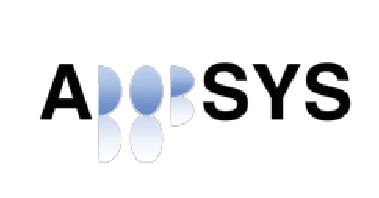
\includegraphics[height=0.55in]{title/logos/adopsys}
\end{center}
\vfill

\noindent
\begin{tabular}{@{}p{0.2\textwidth}@{}p{0.8\textwidth}}
    \textit{Keywords:} & \ldots \\[\medskipamount]
    \textit{Printed by:} & Johannes Gutenberg \\[\medskipamount]
    \textit{Front \& Back:} & Beautiful cover art that captures the entire content of this thesis in a single illustration.
\end{tabular}

\vspace{4\bigskipamount}

\noindent Copyright \textcopyright\ 2022 by Zhe Hou

%% Uncomment the following lines if this dissertation is part of the Casimir PhD
%% Series, or a similar research school.
%\medskip
%\noindent Casimir PhD Series, Delft-Leiden 2013-01

\medskip
\noindent ISBN 000-00-0000-000-0

\medskip
\noindent An electronic version of this dissertation is available at \\
\url{http://repository.tudelft.nl/}.

\newpage
\;
\vspace{12em}



% Here is the explanation about the cover
\begin{figure}[h!]
    \centering
    
\includegraphics[scale=0.35]{cover/CoverSP.png}
\end{figure} 
Designed by Hui Lin

 The concept is borrowed from Escher's style. We draw horse patterns together with the "saddle" which relates to the "saddle point". In between the horse patterns, there are pieces of convex and concave lens shape. I would like to indicate a lens design network or space that the lens solutions are linked/surrounded by saddles (saddle points). In a whole, with Escher's way of presenting, the pattern seems quite complicated, yet is composed with a monotonic repetitive pattern (the feeling of the complexity is probably from the color composition and angular arrangement). It is sort of related to the goal of the thesis/research: in a complicated design landscape, we are trying to find a systematic way to describe it and then utilize knowledge for practical design. 

\end{titlepage}



%% The (optional) dedication can be used to thank someone or display a
%% significant quotation.
\dedication{\epigraph{For my dearest mother\\and for the sake of living without regret}{}} %necessary to keep the empty big parentheses

\chapter*{Preface}
\setheader{Preface}

Preface\ldots

\begin{flushright}
\LARGE\textbf{unnecessary}
{\makeatletter\itshape
    \@firstname\ \@lastname \\
    Delft, January 2013
\makeatother}
\end{flushright}



\tableofcontents

%% Use Arabic numerals for the page numbers of the chapters.
\mainmatter

%% Turn on thumb indices.
\thumbtrue
\chapter*{Summary}
\addcontentsline{toc}{chapter}{Summary}
\setheader{Summary}

In this thesis, we explore how lens design and optimization techniques can adapt to the design (optimization) space in order to increase the lens design efficiency. 

The optical lens design space is known to be very complicated. This is a high-dimensional space defined by the degrees of freedom and the quantified performance of a parameterized optical system. This space is also nonlinear which means there are multiple local minima (you can think of the bottom of a crater in the geological landscape) with different values. In modern optical lens design, the task can be described as searching for the global minimal value in the high-dimensional space. For sophisticated lens designs, the number of the degrees of freedom increases in order to gain more control of the design. It brings two major difficulties:  
\begin{enumerate}[nosep]
\item The size of the high dimensional space increases according to the power law which means a brute force search is practically impossible. 
\item The number of local minima increases with the number of the degrees of freedom used. It indicates the number of undesired local minima becomes larger. Hence, the difficulty of finding best minima also increases.  


\end{enumerate}

% technique has been developed 
Over the past decades, different design and optimization techniques have been examined on their effectiveness of obtaining a global optimal solution. Some of the techniques have been integrated into commercial lens design software. However, these algorithms are based almost exclusively on generally applicable mathematical models and use little or no specific knowledge about the optical system (and its design landscape). As a result, little information is available on how these techniques should be used in a practical design task instead of implementing them as a lottery draw. 

We emphasize in this thesis that, considering an actual lens design process, the design space is not only statically complicated, but also dynamically changes through the design process. The dynamic aspect affects the design landscape. As a consequence, the number of local minima and the effectiveness of the optimization techniques can be impacted. In Chapter \ref{chapter_5_SMS}, a study using Simultaneous Multiple Surface (SMS) method as one of the design strategies, compares the effectiveness of different strategies under static and dynamic design landscape.

Saddle Point Construction (SPC) is a design method which can rapidly construct saddle points with Morse Index 1 in a design space. These saddle points serve as agents to guide the local optimization to obtain new minima. Different from other optimization techniques, it also reveals a special structure in the lens design landscape: certain saddle points existing in the landscape are reducible to minima of simpler systems plus one additional lens element.

Previous research shows potentials of SPC as a systematic lens design technique. In this thesis, we further examine the practicality of SPC as a global optimization and semi-global optimization (to generate a small pool of solutions) tool. The dynamic aspect of the design space is particularly of interest since it is relevant to an actual design practice. 

To assess the robustness of SPC as a global optimization method, we examine the solution network of saddle points and minima for several scenarios. We formulate three falsifiable research questions and have falsified two of them based on the observations:
\begin{enumerate}[nosep]
\item In a lens design landscape, are all the saddle points able to be constructed using SPC? The answer to this question is no. The detail of the analysis is given in Chapter \ref{chapter_SPC_simple_system_landscape}.
\item Are all the minima always linked via the saddle point - minima network revealed by SPC? The answer to this question is also no. The analysis is provided in Chapter \ref{chapter_SPC_simple_system_landscape} and also supported by the wide-angle lens example in Chapter \ref{chapter_4_complex_system_exploration}.
\item Does the saddle points - minima network obtained via SPC always contain the best or the best pool of solutions for lens design? We cannot give an answer to this question. However, in the examples we have examined, the positive side of this question is valid. 
\end{enumerate}

Despite the fact that using SPC does not guarantee capturing all the local minima in the design space, we observe that the good minima are always captured in our examples. Given its systematic way of obtaining local minima, we consider it as a useful global search technique for lens design. 

In addition, in Chapter \ref{chapter_4_complex_system_exploration}, we demonstrate that SPC can be particularly effective for complicated systems when the goal is to get a small pool of solution candidates while the system configuration is not drastically changed. 

\begin{comment}
At last, we provide our thoughts on how the lens design landscape can be further studied. However, it is not straightforward how it can be related to an everyday design task. We believe that a tool gets improved during its practice, therefore, suggestions on further making SPC as a practical lens design tool are also given at the end. 
\end{comment}


\begin{comment}
We analyze the characteristics of the optical lens design space. We emphasize its dynamic property, which means the landscape changes given different design condition is changed, which is a common thing during the design practice

This dissertation addresses the typical problem during optical design or generally all engineering problem -- how to find the best solutions in a parameterized system. 

Goal/Nature of the problem: find the best solution -> assess whether the solution is sufficient or not, if it is not, the process should go to the next design decision; if it is sufficient, the solution can be taken. 

How: Parameterize the system with the multiple variables with a model representing its physical property therefore the performance can be evaluated.  
Given the model, use mathematical tools to optimize in order to get the best solution.
(alternatively, you can realize this by continuous testing and modifying during your manufacture -> caveman's method)

  Sub-problem statement: after parameterization, the optimization space of the system is usually a non-convex space, which indicates a presence of multiple local minima when a typical local optimizer is used. Situation of non-convex space provides difficulties in getting a satisfactory solution: it is difficult to find all the existing solutions in the design space. With incomplete set of information, the following question exist: will there be a better solution if one keeps searching given the current system configuration. As a results, techniques that can quickly generate new solutions given a design configuration is welcome to verify if a better system can be found. The process usually ends when a good enough result is found or a time limit is reached. 

Goal: Find whether there is a better solution in a non-convex optimization problem. This is global optimization. 

How: 
1) starting from a very good starting point (this indicates good technique is needed to construct the starting points) and after arriving at a local minimum, GO technique is used to check whether better solutions can be found (the anticipation is not). 

2) starting from somewhat working point (this indicates small effort to determine the starting point) and combined with GO technique to see if we could find more better solutions. The anticipation is that there would be some better results appear. 

    Sub-problem statement: SPC is a GO technique. SPC shows systematic approach and reveals certain structure between optimization landscape and the optical design model. The following questions are interesting regarding SPC:
1) How SPC is performing as a GO technique? In terms of the completeness and efficiency for finding new solutions. Completeness -> do I find every solution, or at least all solutions find by other algorithms.  Efficiency-> what is the time needed to run such GO. Is it a limited amount of algorithmic trial?
2) Does it show more profound connection to the lens design problem such that it could be used to facilitate the design more? This question should be implicitly included in the first one. It is more of scientific curiosity that if the nature of SPC is connected to the lens design problem. 

    Sub-problem statement: SMS is a starting-point-generating technique. The hypothesis is that it generates a good starting point since the method is guided by the physical rules (Fermat's Principle). Is SMS method the method that providing the starting point that close to the best local minimum (via one local optimizer)? 
    
To sum, it is the balance between the effort of getting a good starting point and running less optimization. SPC as an optimization technique needed to be investigated for its GO efficiency. It means, given a non-perfect starting point, the GO method is preferred to efficiently find the best solution. Chapter 2-4 is trying to clarify this.
SMS as a technique to construct starting points, the ultimate question is that if it constructs the starting point that the minimum optimization effort it needed. Chapter 5 is trying to answer this question. 
\end{comment}
\chapter*{Samenvatting}
\addcontentsline{toc}{chapter}{Samenvatting}
\setheader{Samenvatting}

{\selectlanguage{dutch}

Samenvatting in het Nederlands\ldots

\noindent geschreven worden ...

}


\chapter{Introduction}
\label{chapter_1_intro}
\graphicspath{ {./chapter-sp/figures/} }
\captionsetup[figure]{labelfont=bf}
\captionsetup{margin=1.5em}
\captionsetup[table]{labelfont=bf}


%%Definition of optical design
Optical design, generally speaking, can refer to the activities that manipulate light to achieve a certain purpose. This can be designing a telescope to observe remote celestial bodies, designing a concentrator to maximally harvest the solar energy, or designing optical fibre to maximize efficiency for information transmission. In the community of optical engineering, optical design is commonly associated with optical lens design. That means using optical lenses as the manipulator of light. The focus of this dissertation will also be the design of optical lenses. However, the insights summarized in this dissertation can also be extended to the design with other optical manipulators (e.g. mirrors).

In lens design, the light is usually modeled with its geometrical model(or ray model). The light propagation is described in terms of light rays. When the wavelength of the light is very small compared to the size of the structures with which light interacts, it is an excellent approximation. That also indicates the wave property of light such as interference and diffraction, is not captured by the geometrical model. The utilization of the simpler geometric model is mostly driven by the practicality of optical design: with geometrical optics where light is simplified as rays pointing towards the traveling direction of radiation energy, billion of rays can be traced in seconds for a standard modern personal computer. The performance of the system can be quickly determined for subsequent analysis or optimization. On the other side, with the more rigorous wave model, designing and analyzing a common optical system is computationally expensive, hence very time consuming and inconvenient to rapidly compute and optimize the system performance. 

%(reserved descriptions) However, conventionally, it usually means designing optical systems where light is mainly treated with its geometrical model rather than its more complicated wave model. These optical systems can be a photographic camera, a lamp or a laser beam-shaper, etc.. The aperture sizes of these optical systems are normally from several millimeters to meters. They are very large compared to the operating wavelength of the systems. Therefore, it is safe to apply the geometrical model and it maintains the essence of light that is sufficient to obtain a reasonable optical system design.

%what I want to emphazie is the use of both models, but the description is not well polished.
 % wave model: diffraction limited field analysis - diffraction, interference analysis (highly coherent beams), polarization
 
In some occasions, a wave model is necessary to be applied to understand the system performance. For instance, when an imaging system is only limited by diffraction, analyzing the intensity distribution of a focused beam at the focal plane requires a wave model. A geometrical model will only predict an extreme small spot without the information about the intensity distribution. As a result, depending on the performance requirements, practice for optical system design may involve both geometrical and wave models. A geometrical model is usually used to rapidly obtain a system solution that is good enough in terms of its performance predicted by the geometrical model. When approximation with the geometrical model is no longer accurate, the wave model helps to provide further analysis which gives feedback to fine-tune the system performance. The later part is usually involved in systems with a demanding performance requirement such as microscopic objectives or photo-lithographic projection systems. In this dissertation, the discussion is focused on designing optical systems based on the principles of geometrical optics. The wave model related analysis is not in scope.  


In geometrical optics, one of most important laws would be the law of refraction (also know as the Snell's law). It describes how a light ray travels at the interface of two different media:
\begin{equation}
n \sin i = n^\prime \sin r,
\label{eq: snellslaw}
\end{equation}
where $n$ and $n^\prime$ are the refractive indices of the media before and after refraction of a ray; $i$ and $r$ are the angles of the incidence and refraction at the interface between the two media. According to the law of refraction, lenses are designed to manipulate the light.
\begin{figure}
    \centering
    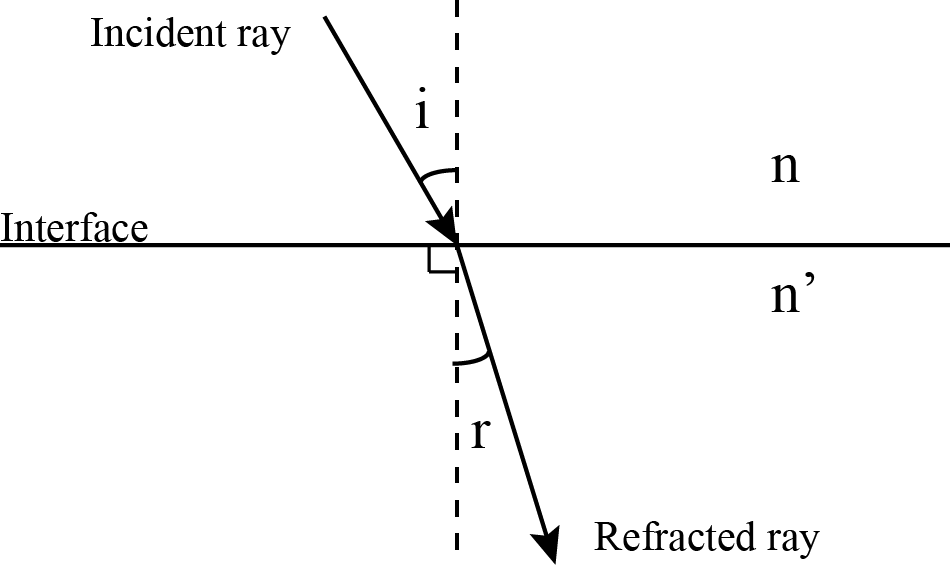
\includegraphics[scale=0.65]{chapter-1/figures/snellslaw.png}
    \caption{Snell's law: the light ray is refracted at the interface between the two media. The relation between the incident ray and the refracted ray is given by Equation \ref{eq: snellslaw}.}
    \label{fig: snellslaw}
\end{figure} 

The earliest known lenses were made by the ancient Egyptians and Mesopotamians \cite{wiki:HistoryofOptics}. They were made from polished crystal, often quartz, and are dated as early as 750BC for Assyrian lenses such as the Nimrud/Layard lens \cite{wiki:Nimrudlens}. The exact function of these lenses is not clear, with some authors suggesting that they were used as an optical lens (magnifying glasses) and others suggesting a decorative function. These lenses were mainly made by trial and error where actual understanding of the light was very limited. When people had more knowledge about geometrical optics, optical design started to pay attention to how light rays travel. With the increasing understanding of the nature of light, the design of optics also evolved from simple lenses to complicated systems which can achieve resolutions down to nanometers. This can not be achieved without the development of modern computer-aided optical design with which the performance of the optical system can be rapidly estimated and numerical optimization can be applied to further improve the system performance.

% background of the lens design approach
In modern optical lens design, an optical system is parameterized in design software. The designer studies the design requirements and determines what the initial configuration of the optical lens should be. Figure \ref{fig:chap0 model design flow} provides a flowchart of a modern optical design process. The optical designer then needs to start modifying the system based on his/her knowledge and observation with a purpose of meeting the design requirements. Numerical optimization, which is widely used in the computer-aid design, is also heavily applied in this step for lens design. With the help of the optimizer, the designer "guides" the system towards a desired configuration. 

\begin{figure}
    \centering
    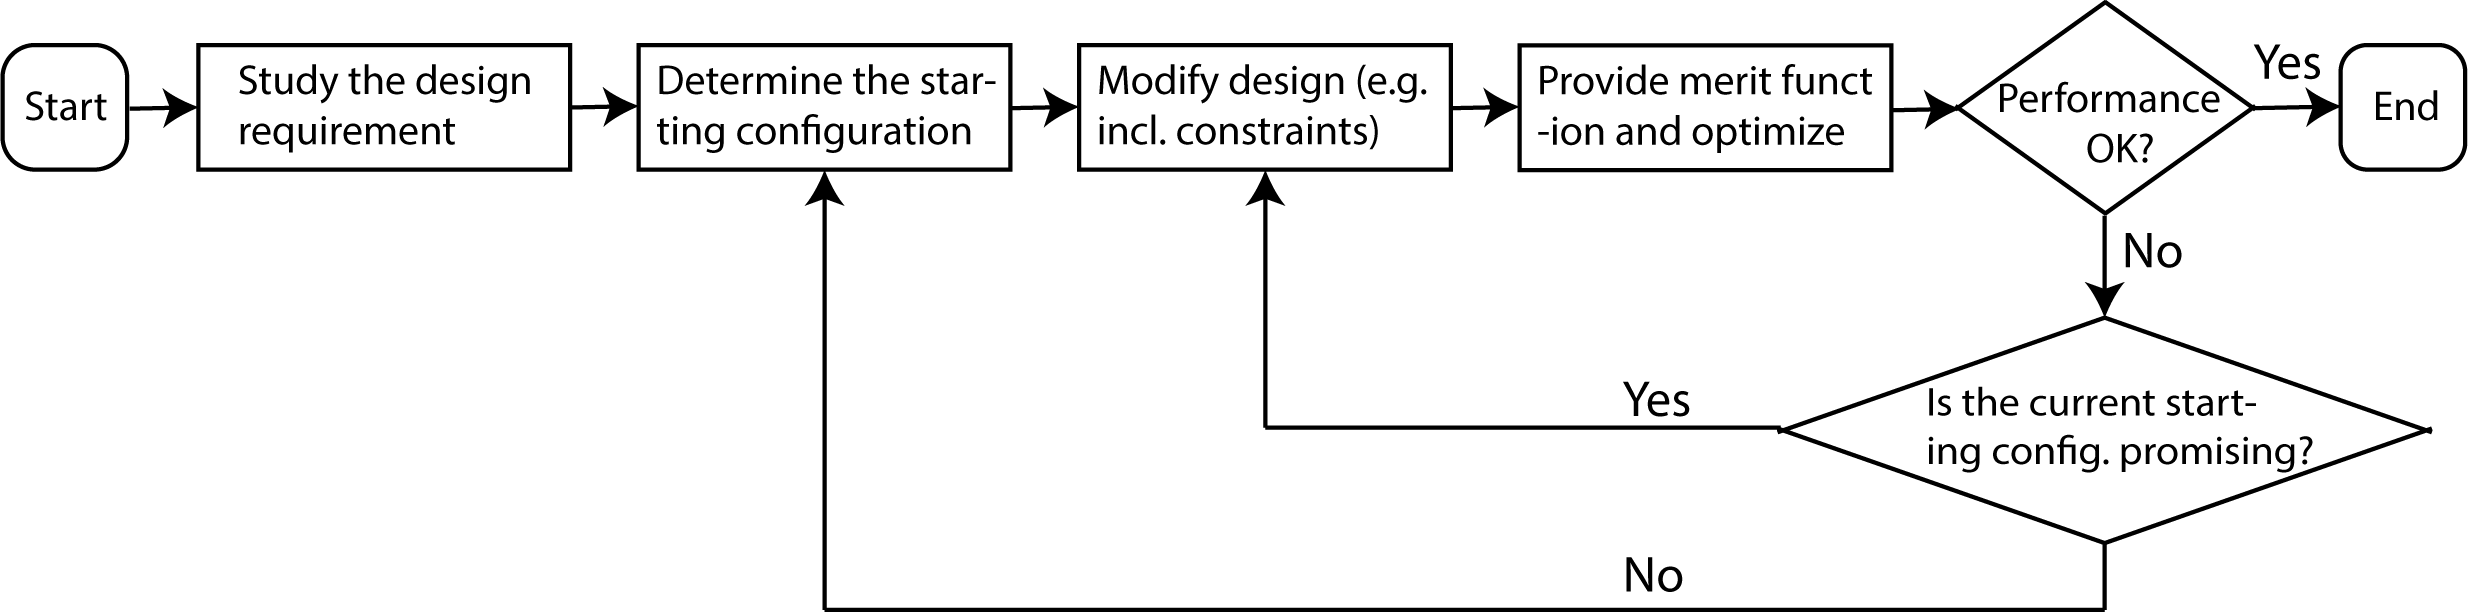
\includegraphics[scale=0.58]{chapter-0/figures/lens_design_flow_chart.png}
    \caption{Flowchart of the modern optical design process.}
    \label{fig:chap0 model design flow}
\end{figure} 

It is now understood and observed that the high-dimensional design (optimization) space formed by the variables of the parameterized optical system are nonlinear. In the terminology of optimization, it means multiple local minima coexist in the design space and the results of a local optimization is sensitive to the choice of its starting point. This presents one of the major challenges of today's optical lens design: to efficiently obtain the global optimal solution among many inferior ones. As the achievable minimum is sensitive to its starting point of the design, this challenge can also be reformulated as: to determine a starting configuration that would land at a global optimal. For complicated systems, finding such optimal starting configurations mostly depends on an optical designer's knowledge and accumulated experience \cite{LivshitsQA2013}\cite{Shafer1995_moreless}. 

The exploration of various global optimization techniques (elaborated in the next chapter) has been given much attention over the last few decades. Given ever-increasing computational power, the hope is that these global optimization tools can lessen the burden on the optical designer by efficiently providing the solution candidates such that the designer can focus on other important tasks instead of trial and error. 

% the gap and how to handle it 
One fact is that these global optimization algorithms rely almost exclusively on generally applicable mathematical models and use little or no specific knowledge about the optical system (and its design landscape). As a result, setting up the proper configurations (similar to the step-size of a local optimizer) of these global optimizer becomes another task of trial and error. 

In this dissertation, we particularly focus on the Saddle Point Construction (SPC) method which uses a special property in the lens design landscape: certain saddle points existing in the landscape are reducible to minima of simpler systems plus one additional element. By investigating how SPC behaves in different design scenarios, we provide insights for systematically design optical systems using SPC. 

% understanding the characteristics of the design landscape is important
% knowing spc and its property to this landscape in order to design is beneficial 

% introducing the dissertation content 

\subsubsection{Outline of the dissertation}
In Chapter \ref{chapter_LensDesign}, we provide some background regarding modern lens design. To better explain a design process, a simple example of designing a magnifying glass is used. We also discuss some of the major optimization techniques available either in commercial design software or publications. 

Chapter \ref{chapter_SPC_method_reccomendation} is dedicated to SPC where we give the mathematical proof for the general version of SPC and explain in detail how SPC could be used in practical lens design. 

In Chapter \ref{chapter_SPC_simple_system_landscape}, a wide-angle pinhole lens design network containing saddle points and minima is given where we demonstrate in one scenario that using SPC can obtain all the minma via the constructed saddle points. However, we further discuss that it is not always valid. When lens design specification changes (e.g. field of view), the design landscape changes correspondingly which alters the number of minima and saddle points that can be retrieved via SPC.  

Lenses with more complexities are used as study examples in Chapter \ref{chapter_4_complex_system_exploration}. For a complex lens system with more number of elements, analyzing the solutions network becomes difficult. In practical design tasks, it is not always necessary to run a global search to list all the solutions in the design space. A small pool of solution candidates without drastically changing the system configurations, could help the design to progress in a more controlled way. We demonstrate in the chapter how SPC can be beneficial in such design scenarios as well as providing some practical insights about the method. 

Chapters \ref{chapter_SPC_simple_system_landscape} and \ref{chapter_4_complex_system_exploration} describe the dynamic aspect of the lens design landscape - instead of remaining static, the design landscape changes continuously through the design process via modifying system specifications, applying constraints, etc. This adds the uncertainty of successfully obtaining a good solution.  In Chapter \ref{chapter_5_SMS}, we deviate from SPC and compare different design strategies for simple aspheric lenses. It is observed that if a good starting configuration including all the constraints and necessary degrees of design freedom can be determined, reaching a global optimal solution can be very efficient. We use Simultaneous Multiple Surface (SMS) method in this chapter to construct such good starting configurations. 

At last, conclusions of the dissertation and some future outlooks are given in Chapter \ref{chapter_Conclusion}.

\references{dissertation}

\begin{comment}

%%%{BACK-UPS
\subsection{Backup notes}
where to insert the lens -> combine with experience 
whether the result is satisfactory -> judge by experience 
controlled way of the getting the solution 

Neural network? 
It is a hot topic so it is good to also mention something about the Neural network work. 
\cite{JM_nn_93}  \cite{Yang:19} \cite{Cote:19}

\section{Problem for optical system design}

When designing an optical system, it is always necessary to consider its source and receiver. When designing imaging system, the object represents the source, where lights from all angles are emitting from the object at each point. The receiver is usually called image, which is normally a flat plane (such as a photosensitive film, or a charged-carrier device sensor). The optical system is located between the source and receiver, after which the light will arrive at the receiver with a designed performance instead of propagate in the air. The source and receiver in a non-imaging system can have more variety: a source can be a simple point source, or can be an extended source with a certain geometrical shape. The receiver can be all kinds of 3D-shape. 

An optical design problem uses all the available components which manipulate the light in a way that it will achieve a certain purpose as the designer desired. This can be either imaging, to focus a point in the object side to the image side with the maximal retained information, or can be non-imaging, to distribute the energy of the light in a way for a certain purpose, such as creating a homogeneous illumination. 

When mentioning optical design, the term is not specified enough. It should be including all the possible way of designing with manipulating light to achieve certain purpose. Regardless of the using of the components or the scale of the components. 

Optical design components, polarizer, diffractive components, multiple aperture (light field camera, cell-phone camera).

The design case mainly handled in this dissertation is the imaging system design, in particular with optical lens design. In this case, the used components are mainly 

\end{comment}


\chapter{Introduction}
\label{chapter_1}
\graphicspath{ {./chapter-sp/figures/} }
\captionsetup[figure]{labelfont=bf}
\captionsetup{margin=1.5em}
\captionsetup[table]{labelfont=bf}

\begin{abstract}
Summary
This dissertation addresses the typical problem during optical design or generally all engineering problem -- how to find the best solutions in a parameterized system. 

Goal/Nature of the problem: find the best solution -> assess whether the solution is sufficient or not, if it is not, the process should go to the next design decision; if it is sufficient, the solution can be taken. 

How: Parameterize the system with the multiple variables with a model representing its physical property therefore the performance can be evaluated.  
Given the model, use mathematical tools to optimize in order to get the best solution.
(alternatively, you can realize this by continuous testing and modifying during your manufacture -> caveman's method)

  Sub-problem statement: after parameterization, the optimization space of the system is usually a non-convex space, which indicates a presence of multiple local minima when a typical local optimizer is used. Situation of non-convex space provides difficulties in getting a satisfactory solution: it is difficult to find all the existing solutions in the design space. With incomplete set of information, the following question exist: will there be a better solution if one keeps searching given the current system configuration. As a results, techniques that can quickly generate new solutions given a design configuration is welcome to verify if a better system can be found. The process usually ends when a good enough result is found or a time limit is reached. 

Goal: Find whether there is a better solution in a non-convex optimization problem. This is global optimization. 

How: 
1) starting from a very good starting point (this indicates good technique is needed to construct the starting points) and after arriving at a local minimum, GO technique is used to check whether better solutions can be found (the anticipation is not). 

2) starting from somewhat working point (this indicates small effort to determine the starting point) and combined with GO technique to see if we could find more better solutions. The anticipation is that there would be some better results appear. 

    Sub-problem statement: SPC is a GO technique. SPC shows systematic approach and reveals certain structure between optimization landscape and the optical design model. The following questions are interesting regarding SPC:
1) How SPC is performing as a GO technique? In terms of the completeness and efficiency for finding new solutions. Completeness -> do I find every solution, or at least all solutions find by other algorithms.  Efficiency-> what is the time needed to run such GO. Is it a limited amount of algorithmic trial?
2) Does it show more profound connection to the lens design problem such that it could be used to facilitate the design more? This question should be implicitly included in the first one. It is more of scientific curiosity that if the nature of SPC is connected to the lens design problem. 

    Sub-problem statement: SMS is a starting-point-generating technique. The hypothesis is that it generates a good starting point since the method is guided by the physical rules (Fermat's Principle). Is SMS method the method that providing the starting point that close to the best local minimum (via one local optimizer)? 
    
To sum, it is the balance between the effort of getting a good starting point and running less optimization. SPC as an optimization technique needed to be investigated for its GO efficiency. It means, given a non-perfect starting point, the GO method is preferred to efficiently find the best solution. Chapter 2-4 is trying to clarify this.
SMS as a technique to construct starting points, the ultimate question is that if it constructs the starting point that the minimum optimization effort it needed. Chapter 5 is trying to answer this question. 


\end{abstract}
%%Definition of optical design
\section{Optical Lens Design}
\vspace{1em}
Optical design, generally speaking, can refer to the activities that manipulate light to achieve a certain purpose. This can be designing a telescope to observe remote celestial bodies, designing a concentrator to maximally harvest the solar energy, or designing a optical fibre to maximize the efficiency for information transmission. In the community of optical engineering, optical design is commonly associated with optical lens design. That means using optical lenses as the manipulator of light. The focus of this thesis will also be the design with optical lenses. However, the insights summarized in this thesis can also be extended to the design with other optical manipulator (e.g. mirrors, phase masks).

In lens design, the light are usually modeled with its geometrical model, or ray model. The light propagation is described in terms of rays. When the wavelength of the light is small compared to the size of structures which light interacts, it is an excellent approximation. That also indicates the wave property of light such as interference and diffraction are not captured by the geometrical model. The utilization of the simpler geometric model is mostly driven by the practicality of optical design: with the more rigorous wave model, designing and analysing an common optical system is computationally expensive, hence   very time consuming and inconvenient to rapidly compute system performance and optimize. On the other side, with geometrical optics where light is simplified as rays pointing towards the traveling direction of radiation energy, billion of rays can be traced in seconds for a standard modern personal computer. The performance of the system can be quickly determined for subsequent analysis or optimization.   

%(reserved descriptions) However, conventionally, it usually means designing optical systems where light is mainly treated with its geometrical model rather than its more complicated wave model. These optical systems can be a photographic camera, a lamp or a laser beam-shaper, etc.. The aperture sizes of these optical systems are normally from several millimeters to meters. They are very large compared to the operating wavelength of the systems. Therefore, it is safe to apply the geometrical model and it maintains the essence of light that is sufficient to obtain a reasonable optical system design.

%what I want to emphazie is the use of both models, but the description is not well polished.
 % wave model: diffraction limited field analysis - diffraction, interference analysis (highly coherent beams), polarization
 
In some occasions, wave model is necessary to be applied to understand the system performance. For instance, when an imaging system is only limited by diffraction, the intensity distribution of a focused beam at the focal plane requires wave model. Geometrical model will only indicate an extreme small spot without the information about the intensity distribution. As a result, depends on the performance requirements, practice for optical system design may involve both geometrical and wave model. Geometrical model is usually used to rapidly obtain a system solution, which fulfill the requirements on the level of geometrical model. When approximation with geometrical model is not accurate anymore, wave model helps to provide further analysis result which gives feedback to fine-tune the system performance. The later part may only involved in systems with demanding performance requirement such as microscopic objectives or lithographic projection systems. In this thesis, the discussion is focused on the part of designing optical systems based on the principles of geometrical optics. The wave model related analysis is not in scope.  
%
In geometrical optics, one of most important law would be the law of refraction (also know as the Snell's law). It describes the how a light ray travels at the interface of two different media:
\begin{equation}
n \sin i = n^\prime \sin r,
\label{eq: snellslaw}
\end{equation}where $n$ and $n^\prime$ are the refractive indices of the media before and after refraction of a ray; $i$ and $r$ are the angles of the incidence and refraction at the interface between the two media.
\begin{figure}
    \centering
    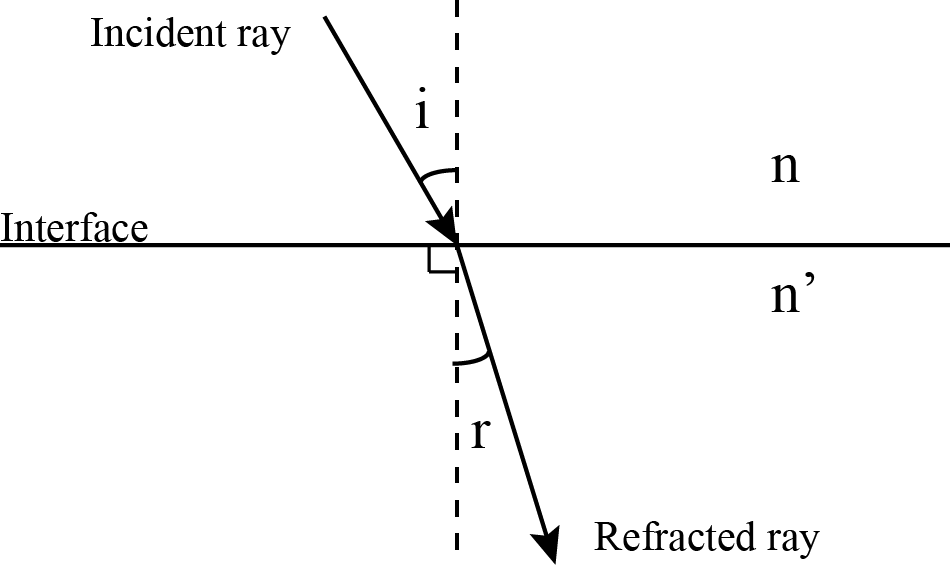
\includegraphics[scale=0.58]{chapter-1/figures/snellslaw.png}
    \caption{Snell's law: the light ray is refracted at the interface between the two media. The relation between the incident ray and the refracted ray is given by Equation \ref{eq: snellslaw}.}
    \label{fig: snellslaw}
\end{figure} 

The earliest known lenses were made by the ancient Egyptians and Mesopotamians \cite{wiki:HistoryofOptics}. They were made from polished crystal, often quartz, and have dated as early as 750BC for Assyrian lenses such as the Nimrud/Layard lens \cite{wiki:Nimrudlens}. The exact function of these lenses is not clear, with some authors suggesting that it was used as an optical lens (magnifying glasses) and other suggesting a decorative function. These lenses were mainly made by trial and error where actual understanding of the light was very limited. When people had more knowledge about geometrical optics, optical design started to involve calculating how light rays travel. With the increasing understanding of the nature of light, the design of optics also evolves from simple lenses to complicated systems which can achieve resolutions down to nanometers. In the following subsection, we will use a simple example of an magnifying glass to sketch how optical design works.     

%Useful reference, https://opentextbc.ca/universityphysicsv3openstax/chapter/the-simple-magnifier/%
\subsubsection{Example of designing a Magnifying Glass} \label{magnifier}
\vspace{1em}
Let us start with an example of designing a magnifying glass, whose application can be assisting reading. Assume the magnification requirement of the magnifier is $6\times$. We know from text book \cite{hecht2012optics} that such a magnifier can be made using a convex lens. The magnified image is a virtual image that is then captured by the human-eye. The magnification of a magnifier is defined as the angular magnification which is the ratio between the subtended angles to the eye of the object and the image. This is illustrated in Figure \ref{fig: geo_formulae}-(a). A larger angle means a larger image is formed on the retina of the eye. The object and image are normally located at a distance of $250 mm$ from the eye. The distance represents the near-point, which is the closest distance that the eye can view comfortably. 
% illustration of the angular magnification


Figure \ref{fig: geo_formulae}-(b) shows how the virtual image is formed considering an ideal thin lens scenario. Certain rules are used to derive such a plot:
1) A light ray, which starts from the object plane and is parallel to the optical axis, will pass the focal point at image side;
2) A light ray, which starts from the object plane and passes the nodal point (the intersection between the ideal lens and the optical axis), will remain its original direction.

In this thesis, we use the following convention for the geometrical optics formulas: points (object, image or focal point) sitting on the left side of the lens has a negative distance to the lens. Points sitting on the right side of the lens has a positive distance. The radius of the optical surfaces is positive when the center of curvature is to the right of the surface vertex, and vice versa. 

\begin{figure}
    \centering
    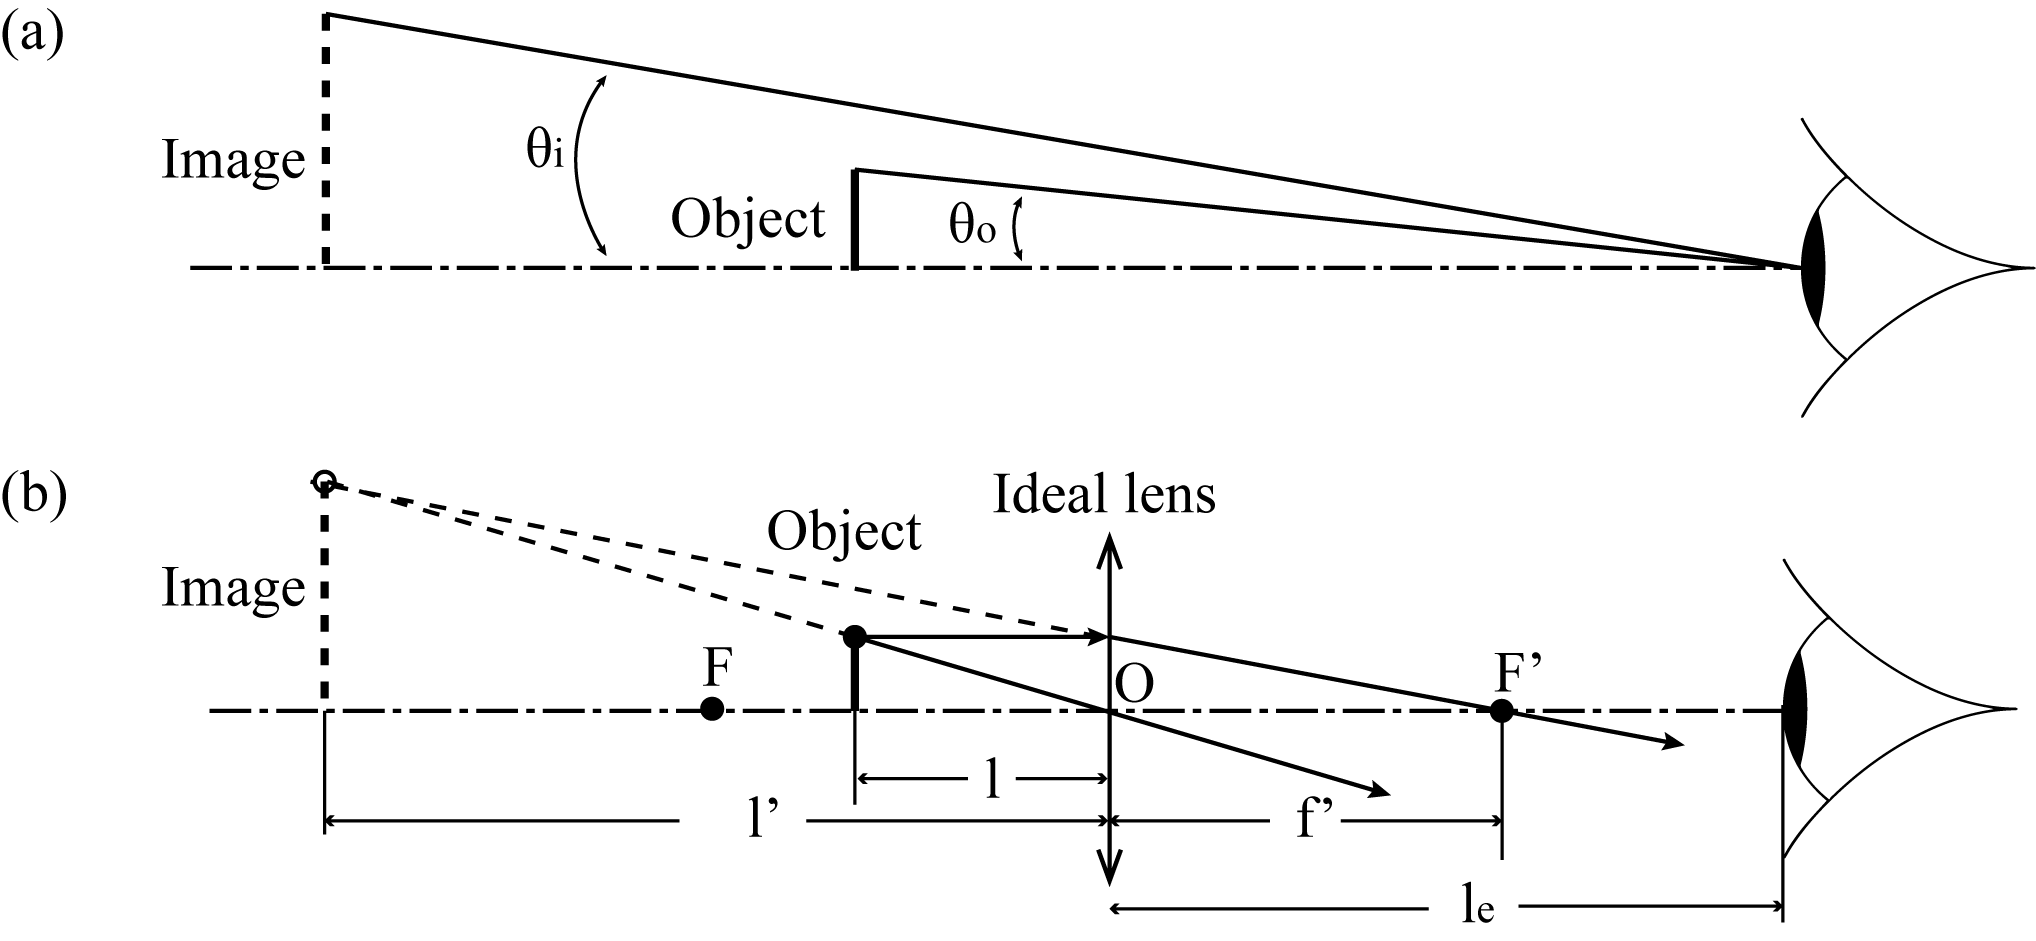
\includegraphics[scale=0.58]{chapter-1/figures/geo_magnifier_v2.png}
    \caption{(a) The magnification of a magnifying glass is defined as the ratio between the image subtended angle $\theta_{i}$ and  the object subtended angle $\theta_{o}$.  
    (b) Illustration of a virtual, enlarged image of the object through a magnifying glass. Equations \ref{eq: thinlensformula} - \ref{eq: magnifier magnification} explain the relation of the parameters.}
 %(b) Illustration of the Lensmaker's equation. For thin lens case, the equation is given by \ref{eq: lensmaker_r}. The thick lens case equation is given by \ref{eq: lensmaker_r_thick}.
    \label{fig: geo_formulae}
\end{figure} 

The subtended angle $\theta_o$ of the object to the eye writes 
\begin{equation}
\label{eq: magnifier object angle}
\theta_o = \frac{h_o}{250 \; mm},
\end{equation}where $h_o$ stands for the height of the object.
The subtended angle $\theta_i$ of  the magnified image writes
\begin{equation}
\label{eq: magnifier image angle}
\theta_i = \frac{mh_i}{l_e-l'},
\end{equation}where $m (= \frac{l'}{l})$ is the lateral magnification and $l_e$ is  the distance from the eye to the lens. Since the image is virtual ($l'<0$), the expression $l_e - l'$ indicates the distance between the image and the eye. Together with the thin lens equation 
\begin{equation} \label{eq: thinlensformula}
    \frac{1}{l^\prime} - \frac{1}{l} = \frac{1}{f^\prime},
\end{equation}we can write Equation \ref{eq: magnifier image angle} into
\begin{equation}
\label{eq: magnifier image angle reform}
\theta_i = (1-\frac{l'}{f'})\cdot\frac{h_o}{l_e-l'}.
\end{equation}With Equation \ref{eq: magnifier object angle} and Equation \ref{eq: magnifier image angle reform}, the magnification $m_{mag}$ of the magnifier is 
\begin{equation}
\label{eq: magnifier magnification}
m_{mag} = \frac{\theta_i}{\theta_o} = (1-\frac{l'}{f'})\cdot\frac{250 \; mm}{l_e-l'}.
\end{equation}The distance between the image and the eye $l_e-l'$ can be set as $250 \;mm$. For the maximum $m_{mag}$, we have $l' = -250 \; mm, l_e \approx 0$. It means that when the eye is observing close to the magnifier, the maximum magnification of the image is achieved. This magnification is
\begin{equation}
\label{eq: magnifier magnification simplified}
m_{mag}  = 1+\frac{250 \; mm}{f'}.
\end{equation}Now we substitute $m_{mag}$ with $6$, then we have $f' = 50 \; mm$. As a result, we need a magnifying glass with a focal length of $50 \;mm$ to achieve a magnification of  $6\times$.
%% use the following equation to derive lens shape 2021-09-28
Now we know the focal length  $f' = 50 \; mm$ and the image distance $l' = -250 \; mm$. Given Equation \ref{eq: thinlensformula}, the object distance is calculated to be $41.67 \;mm$.  

For a spherical lens, the radii of the two spherical surfaces of the lens can be calculated using Lensmaker's equation 
\begin{equation} \label{eq: lensmaker_r}
    (n-1)(\frac{1}{R_1} - \frac{1}{R_2}) = \frac{1}{f^\prime},
\end{equation}
where $n$ stands for the refractive index of the lens material. $R_1$ and $R_2$ are the radii of the two spherical surfaces. The focal length $f^\prime$ is $50 \; mm$. Let us use a common optical material such as BK7 glass. It has a refractive index ($n$) of approximately $1.5$ in the visible spectrum. For simplicity, we use $1.5$ as our refractive index value.

Now in Equation \ref{eq: lensmaker_r}, the two radii can still vary and we do not have a unique set of values to satisfy the equation. We can choose to have a double-convex lens by forcing the absolute radii to be identical, where $R_1 = 50 \; mm$, and $R_2 = -50 \; mm$. 

Equation \ref{eq: lensmaker_r} assumes the thickness of the lens is very small compared to the radius of the two surfaces (a thin lens scenario). There is also the equation when the thickness $d$ of the lens is considered:
\begin{equation} \label{eq: lensmaker_r_thick}
    (n-1)\left( \frac{1}{R_1} - \frac{1}{R_2} + \frac{(n-1)d}{nR_1R_2} \right) = \frac{1}{f^\prime}  .
\end{equation}
With a thickness $d$ of $3 \; mm$, the radii can be now calculated using Equation \ref{eq: lensmaker_r_thick} to be$R_1 =  49.50 \; mm$ and $R_2 = -49.50 \; mm$. These values are very close to the case when using thin lens approximation ($50 \; mm$ and $-50 \; mm$). 
At this phase, the above derivation shows that based on first order (Gaussian) optics, the following specification can achieve a magnification factor of $6\times$, given that the object locates $41.67 \; mm$ from the lens:

\begin{table}[h!]
    \centering
    \captionsetup{justification=centering}
    \caption{Magnifying Lens Specification}
    \label{magnifying lens specs}
    \vspace{-1em}
    \begin{tabular}{ p{15em}  c }
    \hline 
    Magnification & 6 $\times$\\ 
    Number of lens & 1\\ 
    Diameter & 25 mm\\ 
    Refractive index & 1.5\\ 
    Thickness & 3 mm\\ 
    Radii & 49.50 mm, -49.50 mm\\
    Effective focal length & 50 mm\\
    \hline
    \end{tabular}
\end{table}
 
For the aforementioned example, we used the most basic Lensmaker's formula to design a $6 \times$ magnifier with a double-convex lens.  The condition of double-convex is chosen by us since according to Equation \ref{eq: lensmaker_r_thick}, there are infinite choices of radii that satisfy the equation. Note that the Lensmaker's formula is based on first-order optics, where the angle between the rays and the optical axis is assumed to be very small. This assumption does not hold anymore when optical aberration needs to be treated. In the following part, we show an example on how to improve the magnifier design considering minimizing the spherical aberration.  

The primary monochromatic aberration are the spherical aberration, coma, astigmatism, field curvature and distortion. There are axial and lateral chromatic aberrations when chromatic application is considered. Given the thin lens model, the coefficient of each aberration term can be explicitly expressed. The term of the spherical aberration can be expressed as:
\begin{equation} \label{eq: Si_spherical}
    S_I = \frac{h^4}{4{f^\prime}^3}\left(\frac{3n+2}{n}M^2 - \frac{4(n+1)}{(n-1)n}XM + \frac{n+2}{(n-1)^2n}X^2 + \frac{n^2}{(n-1)^2}\right).
\end{equation}                            %% Figure illustration of the spherical aberration. I don't think I need to add it. 21/09/18%
where $h$ indicates the ray height on the lens surface. $X$ stands for the bending factor of the thin lens (\cite{GrossHBOvol1}, 10.1.1):
\begin{equation} \label{eqn: bending factor}
X = \frac{R_1+R_2}{R_2-R_1},
\end{equation}and $M$ stands for the position parameter (\cite{GrossHBOvol1}, 10.1.2):
\begin{equation} \label{eqn: position parameter}
M = \frac{1+m}{1-m},
\end{equation}$m$ is the magnification factor and it is $6$ as defined previously. In this case, $M=-\frac{7}{5}$. In Equation \ref{eq: Si_spherical}, for a chosen ray, parameter $f^\prime$, $M$, and $n$ are all given. Therefore, $S_I$ becomes a quadratic function for the bending factor $X$. There is a value of $X$ that minimize the value of $S_I$. In this case, when $X = -1$ , the minimum value of $S_I $ is $ 8.16(\frac{h^4}{4(f^\prime)^3})$. The spherical aberration of each ray is proportional to its ray height given the fixed lens configuration. 

Now if we consider both the Lensmaker's equation \ref{eq: lensmaker_r} and the spherical term in Equation\ref{eq: Si_spherical}, the two radii of the lens can be solved as $R_1 = \infty, R_2 = -25\ mm$. These two values are very different from the values ($50 \ mm$ and $-50 \ mm$) calculated based on first-order optics. It is worth mentioning that Equation \ref{eq: Si_spherical} assumes a thin lens, hence the comparison of the radii is done between thin lens models. It is also observed that in our magnifier example, considering a $3 \;mm$ lens thickness in Lensmaker's formula does not alter the radii significantly.  

When more aberration terms are considered, the number of variables in this example is not enough to analytically solve the values for the minimal values of each aberration term. Normally, new degrees of freedom will be introduced to the system (e.g. adding new lenses). However, more number of variables also implies an increasing complexity of the formulae. Modern optical design handles it by using computer-aided design techniques. Numerical optimization and rapid ray tracing are done by computers, which improves the efficiency of optical design.  


\section{Modern Optical Design}
\vspace{1em}
Prior to the development of digital computers, lens optimization was a hand-calculation task using trigonometric and logarithmic tables to plot 2-D cuts through the multi-dime-nsional space. As the development of the digital computer in the 20th century, it drastically shapes the way how optical design is being practised. The burden of calculation is tremendously reduced by using computers. Instead of calculating each ray path on paper,  optical systems are parameterized into different variables representing the physical construction of an optical system (a physical model). For example, a simple two-element air-spaced spherical lens can be represented with nine variables (four radii of curvature, two thickness one airspace, and two glass types). With increasing complexity (number of elements, type of surfaces) of the system, the number of variable can reach hundreds. Using modern computers allows rapid ray tracing calculation by which the performance of the lens system can be quickly modelled and evaluated. 

Helped by the technique of numerical optimization, the vast high-dimensional design space can be searched to look for the set of variables providing the optimal performance of the system. Lens optimization has been studied as early as the 1940s \cite{wikilensdesign}. The earliest attempt for optimizing a doublet using computer dates back to 1950s, when James G. Baker used the \textit{Harvard Card Programmed Calculators} \cite{ThompsonOpticalDesignHistory}.  A good description of the starting of computer-aided optical design is given in a 1963 paper by Feder \cite{Feder:63}. In order to optimize an optical system using the computer, a merit function is necessary to be constructed. The value of this merit function predicts the performance of the system. Normally, the smaller the value of the merit function, the better the performance should be. For an imaging system, such a merit function can be the sum of the aberrations, the size of the focused spot, etc.  The merit function in optical design is commonly defined as \cite{GrossHBOvol3}:
\setlength{\belowdisplayshortskip}{5pt}
\setlength{\abovedisplayshortskip}{5pt}
\begin{equation} \label{eq:MFdefi}
MF(\pmb{x})=\sum_{j=1}^{m} w_j [\tilde{f}_j(\pmb{x}) - \tilde{f}_{tar,j} ]^2,
\end{equation}
\noindent where $\textbf{x} = (x_1, x_2, ..., x_N)$ is a vector describing a point in the $N$-dimensional variable space. $\tilde{f}_j(\textbf{x})$ are the operands with target values $\tilde{f}_{tar,j}$. $\tilde{f}_j(\textbf{x}) - \tilde{f}_{tar,j}$ could be defined as elementary aberration such as ray or wavefront deviations for selected rays. $w_j$ are the positive weighting factors, therefore $MF$ is a single number giving the residual of various operands and their target values. The weights and targets can be absorbed in the definition of the operands, therefore we have 
\begin{equation} \label{mf_oprand_vector}
MF(\pmb{x}) = \pmb{f}^{T}(\pmb{x})\cdot \pmb{f}(\pmb{x}),
\end{equation} where $\pmb{f}$ is a vector having the operands as components.

Given the merit function, a high dimensional space is determined. Each sets of value of the variables represents a point in this high dimensional space and the value of the merit function is determined at that point. Ideally, the value of the merit function is directly associated with the performance of the optical system is being designed. The minimal value of the merit function is desired because it represents the best system performance. 

Once the variables are chosen from the system, the next step is to apply numerical optimization techniques to minimize the value of the merit function defined in Equation \ref{eq:MFdefi}:
\begin{equation} \label{eq:MFopt_cp1}
\begin{split}
& \text{minimize}\;\; MF(\pmb{x}) ,\\
& \text{subject to some constraints},
\end{split}
\end{equation}
with optimization, a new set of values of the variables $\pmb{x_{opt}}$ is obtained such that the value of the merit function is a minimal.

As shown in the example of the magnifier, in order to fulfill the requirements of working distance, magnification and at the same time minimize the spherical aberration for a thin lens model, the radii of the optical surfaces have been calculated. However, in practice, spherical aberration is not the only aberration contributor that limit the image performance. At the same time, some thickness of the lens needs to be added for practical reasons. Given the previously calculated radii and other parameters of the magnifier, a merit function value can be determined after the lens is modeled in an optical design software. This merit function value usually can be further reduced for better system performance with optimization techniques.  

We applied optimization in optical design software CODE V with the magnifier example. Three different cases are parameterized in CODE V as starting points for the optimization. The variables are the two radii of the surfaces. The thickness is also used as a constrained variable to optimize a thick lens. The radii and merit function in each step of the optimization of the three cases are listed in Table \ref{tb: magnifier optimization}. 
% to do: 1) to add the merit function in the table.  2) good to have, to have the plot of the systems
% the magnification of the magnifier is the defined typically as the angular magnification, so the model need recalcualtion, but the process should be the same !!!!!!! 09/23. Need further continuation on the topic after fix the magnification definition  

In CODE V, the working distance is set as $30 \; mm$,  the magnification is constraint as $3$ and the object height are chosen as $0 \; mm$, $1.8 \; mm$ and $2.5 \; mm$. When optimized directly with the input setting, both thin lens approximation with paraxial optics and optimized spherical aberration converge to the same local minimum. Then, the thickness of the thin lens is gradually increased to 5 mm while optimizing the system. Three starting points all converge to the same local minimum. After that, we increased the field by adding non-axial object height. The radii changed slightly. From the table, it is seen that when optimizing in CODE V under the given condition, it makes no difference among the three starting points. All of  them in this case leads to the same local minimum. As a relative simple design problem, it is not sensitive to the choice of starting point.

\newcolumntype{M}[1]{>{\centering\arraybackslash}m{#1}}
\begin{table}[h!]
	\small
    %\centering
    \captionsetup{justification=centering}
    \caption{Optimization results of the Magnifier in CODE V}
    \label{tb: magnifier optimization}
    \vspace{-1em}
    \begin{tabular}{|M{2.7cm}|M{1.9cm}|M{1.9cm}|M{1.9cm}|M{1.9cm}|}
    \hline
                           & \multicolumn{4}{c|}{Radii (mm)}\\ \cline{2-5}
  \textbf{Starting point} & Original& Thin lens, 0 object height & Thick lens, 0 object height & Thick lens (5 mm),  2.5 mm object height\\  \hline
   \textbf{Thin lens approx.}  & 45, -45 & -116, -19 & &\\  \cline{1-3}
    \textbf{Thick lens} & 44, -44& / & \multirow{3}{*}{-203, -23} & \multirow{3}{*}{-196, -23}\\  \cline{1-3}
    \textbf{Thin lens optimized for spherical aberration} & -105, -19& -116, -19& &\\ 
    \hline
    \end{tabular}
\end{table}

In summary, the process of the modern optical design can be generally separated into two steps: 1) determine configurations of the system as starting points; 2) use computational model to optimize the system performance. Mastering both steps requires a good understanding of the optical systems as well as in-depth knowledge of optimization. We will explain these two parts in the following sections, with an emphasis on the optimization techniques. 

\subsection{Optical System Optimization }
\vspace{1em}
When the optical system and its merit function are treated as an optimization problem, there are two kinds of situations: 1) the merit function is a \textit{convex} function \footnote{Geometrically, a function is \textit{convex} if a line segment drawn from any point $(\pmb{x}, f(\pmb{x}))$ to another point $(\pmb{y}, f(\pmb{y}))$ -- called the \textit{chord} from $\pmb{x}$ to $\pmb{y}$ -- lies \textit{on or above} the graph of $f$.} and there is only one global minimum; 2) the merit function is a \textit{non-convex} function and there are multiple local minima. 

Simple cases such as the Magnifier example, the spherical aberration is a quadratic function of the bending factor.  The given number of equations equals the number of variables. An extract solution can be solved. However, in optical design, the common situation is that the number of equations is larger than the number of variables \footnote{In terms of ray tracing, each ray becomes an equations of the given variables. Hundreds of rays are normally traced for calculating the merit function.}. In this case, an approximation of the solution can be given. This is achieved by local optimization, where one minimum can be acquired. 

It is also observed that when the number of the variables (e.g. the number of lenses) increases, the number of the solutions also increases \footnote{A good example is illustrated in Page 61 of Reference \cite{vanTurnhoutThesis2009}. The contour plot of the merit function of a doublet with respect to two variables shows four local minima.} This is because the merit function becomes \textit{non-convex} as the variable increases. The results of the local optimization is then sensitive to the initial point where optimization starts.  

\subsubsection{Basins of attraction \label{label: basinOfattrac}}
\vspace{1em}
In an optimization problem, the basin of attraction defines a set of points in the optimization space, where the optimization leads to the same local minimum. An example of a one-dimensional merit function and its corresponding basins of attraction is given in Figure. ref\{fig: basinOfattraction}. 

\begin{figure}
    \centering
    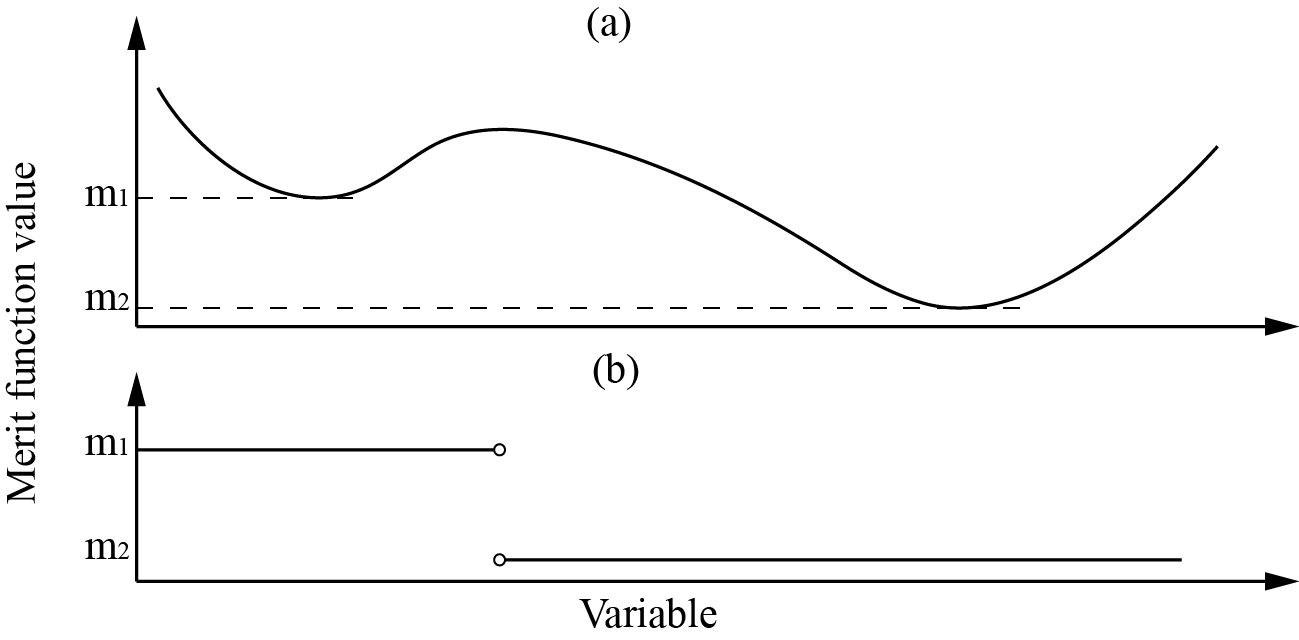
\includegraphics[scale=0.58]{chapter-1/figures/basinOfattraction.png}
    \caption{Illustration of basins of attraction in a one-dimensional optimization space. (a) The merit function with two local minimum having value $m_1$ and $m_2$ . (b) The corresponding basins of attraction in the plotted merit function region. At the boundary of the two basins, it is unclear where the optimization leads to, therefore marked as circles.}
    \label{fig: basinOfattraction}
\end{figure} 

The illustration of the basin of attraction is a direct way to visualize how optimization results in the optimization space, especially in a non-convex problem \footnote{In Chapter 4, basins of attraction on the two-dimensional hyper-plane are used for demonstration purpose. }. The result of a local optimizer is determined by its starting point. Since the goal of this problem is to find the global minimum among the many, there are two consequent strategies: 
1) start from the basin of attraction that corresponds to the global minimum; 
2) search for all (most of) the basins of attraction, list all the minima and obtain the global minimum.

In optical design, the former one is largely associated with the conventional optical design strategies. The starting point can be determined from the literature and patent data, where the system is believed to have a larger chance to lead to a satisfactory minimum. Another approach is to compute the system parameters based on analytical model. The assumption is that the starting point provided by the analytical model is in the basin of attraction of the global minimum.  However, when the optical system becomes increasingly complicated, e.g. adding lenses, making surfaces aspheric, etc., it is very difficult to fully analysing the system and providing a starting point. The strategy of finding multiple minima and selecting the best among them becomes more preferred in this situation. 

The most straightforward method to search for the global minimum is to systematically evaluate the merit function value on the multi-dimensional grid. The problem of this method is that the computational time increases exponentially with the number of variables. By applying a local optimizer, the amount of merit function evaluations can be reduced when starting from a basin of attraction. The task of finding the global minimum is then transformed to finding the basin of attraction containing the global minimum. 

\subsection{Getting the starting point}
When multiple minima presented in the optical design space, the result of the local optimization is sensitive to its choice of the starting point. In the conventional optical design practice, large effort is spent on obtaining a good starting point. 

As demonstrated in the beginning of this chapter, simple systems such as the Magnifier can be computed using first-order optics and third-order aberration model to obtain a relative good starting point. For more complicated systems which contain more optical elements and difficult requirement, there are design strategies summarized by lens designers based on their in-depth knowledge and extensive experience \cite{LivshitsQA2013}\cite{Shafer1995_moreless}. However, mastering these design methods can require year of practice.   

A common practice is that optical designers scan through the existing catalog of the available designs. This can be via patent search or by looking up examples in the optical design books \cite{smith1992modern} \cite{book:SmithModernOpticalEngineering}.  The one has the closest specification with respect to the design requirement is chosen to serve as the  starting point of the design. The assumption is that this chosen system is already in the basin of attraction where good system performance is expected. By doing some fine adjustment, the preferred system should be achievable. 

Methods such as Simultaneous Multiple Surface (SMS) method \cite{MinanoOE09}, which obtains a starting point based on iterative ray tracing process, have also been getting many attentions recently. The SMS method can be very effective for obtaining starting points consisting of aspherical lenses. In Chapter 5, we will look at the SMS method and the corresponding design landscape. 

\subsection{Local optimization}
\vspace{1em}
Given the starting point and the merit function, the local optimizer aims to find a local minimum (minimization problem) where the value of the merit function does not increase anymore. Numerically, this is achieved by iterative steps. In the \textit{N} dimensional space, the local optimization process consists of moving from the starting point towards the minimum in several steps. The value of merit function reduces after each step, until a minimum is reached. When close enough to a minimum, further iteration will not produce any significant changes in  the system parameters and the process is called convergent. 

\newline

\textbf{General problem statement}

Given the $j$-th component, $f_{j}(\pmb{x})$, of the operands vector $\pmb{f}$ can be written as the following formula with a Taylor expansion 
\begin{equation} \label{mf_taylor_expansion}
f_{j}(\pmb{x_0}+\Delta\pmb{x}) = f_{j}(\pmb{x_0}) + \Delta\pmb{x}^T\cdot \nabla f_{j}(\pmb{x_0}) +\frac{1}{2}\Delta\pmb{x}^T\cdot H_{j} \cdot \Delta\pmb{x},
\end{equation} where $\Delta\pmb{x}$ describes the size and direction at a certain optimization iteration. $H_j$ is the Hessian matrix of $f_j$ at $\pmb{x} = \pmb{x_0}$. Its elements are 

\medskip
\newline
\begin{center}
$
\left( H^N_{j} \right) = 
\begin{bmatrix}
\frac{\partial^2 f_j}{\partial{x_{0,1}^2}} &    \cdots          & \frac{\partial^2 f_j}{\partial{x_{0,1}\partial{x_{0,N}}}}    \\
       \vdots                   &     \ddots            & \vdots \\
\frac{\partial^2 f_j}{\partial{x_{0,N}\partial{x_{0,1}}}}     & \cdots           & \frac{\partial^2 f_j}{\partial{x_{0,N}^2}} \\
\end{bmatrix}
$.
\end{center}
\medskip
%A control function of $\Phi(\pmb{x})$ 
The merit function in Equation \ref{mf_oprand_vector} can be written at $\pmb{x}$ in the vicinity of $\pmb{x_0}$ using Taylor expansion :
\begin{equation} \label{mf_expanded}
MF(\pmb{x}) = \pmb{f_{0}}^{T} \cdot \pmb{f_{0}} + 2 \Delta x^{T} \cdot \pmb{J}^{T} \cdot \pmb{f_{0}} + \frac{1}{2} \Delta x^{T} \cdot \pmb{H} \cdot \Delta x,
\end{equation}where $\pmb{f_0} = \pmb{f}(\pmb{x_0})$, $\pmb{J} = \nabla \pmb{f}(\pmb{x})\vert _{\pmb{x} = \pmb{x_0}}$, which is the Jacobian matrix of $\pmb{f}$ at $ \pmb{x} = \pmb{x_0} $ (with elements: $J_{ij} = \frac{\partial{f_i}}{\partial {x_j}} \vert _{x_j = x_{j,0}}$), $\pmb{H} = 2 \left( \pmb{J}^T \cdot \pmb{J} + \sum_{j=1}^{m} f_j(\pmb{x_0}) \cdot H_j \right) $, which is the Hessian matrix of $MF$ at $ \pmb{x} = \pmb{x_0} $. 
To find the minimum of $MF(\pmb{x})$ , numerical iteration steps are executed. The gradient of $MF$ with respect to the optimization variables vanishes
\begin{equation}\label{eq: MF_grad_zero}
\nabla MF(\pmb{x}) = 2 \pmb{J}^{T} \cdot \pmb{f_0} + \pmb{H} \cdot \Delta x = 0.
\end{equation}Different methods are used to solve this equations. We mention here the most common ones. 
\newline

\textbf{Newtonian method}

The Newtonian methods solve the Equation \ref{eq: MF_grad_zero}. The computation of the Hessian matrix $\pmb{H}$ is expensive. As a result, approximation of the Hessian matrix is usually used. The Gauss-Newton method is a common method, where the $H$ is approximated by $2\pmb{J}^T \cdot \pmb{J}$ . The Equation \ref{eq: MF_grad_zero} can then be written as 
\begin{equation} \label{eq: gauss-newton}
\begin{align}
2 \pmb{J}^{T} \cdot \pmb{f_0} + 2\pmb{J}^T \cdot \pmb{J} \cdot \Delta x = 0 , \\
\Delta x = - (\pmb{J}^T \cdot \pmb{J} )^{-1} \cdot \pmb{J}^{T} \cdot \pmb{f_0},
\end{align}
\end{equation}
where $\Delta x$ is the steps used for iteration calculation. 
The advantage for Newtonian method is that it converges fast when the operands are linear (in the vicinity of a local minimum). However, when starting far from the local minimum, the operands are usually very nonlinear. In such cases, it may be difficult for the algorithm to find the vicinity of a local minimum. 
\newline

\textbf{Steepest descent}

The method of steepest descent  ignores the second order term and only uses the first order term for  Equation \ref{mf_expanded}. The step for the numerical optimization is defined with a negative direction towards the gradient of the function. If we start the optimization at $\pmb{x_0}$, the step can be written as
\medskip
\newline
\begin{center}
$
\Delta x = - t \cdot \nabla MF(\pmb{x_0}), \;\; \pmb{x} = \pmb{x_0} + \Delta x,
$
\end{center}
\medskip
where $t>0$, represents the size of the step. We define a function of $t$ as 
\begin{equation} \label{eq: function of t}
\phi(t) = MF(\pmb{x_0} - t \cdot \nabla MF(\pmb{x_0})).
\end{equation}The derivative of $\phi(t)$ at $t=0$ is
\begin{equation}\label{t=0}
\phi'(0) = - \vert\vert \nabla MF(\pmb{x_0}) \vert \vert < 0.
\end{equation}Given $MF(\pmb{x})$ is continuous differentiable, for $t>0$, we have $\phi(t) < \phi(0)$. Hence, we have
\begin{equation}
MF(\pmb{x_0}) > MF(\pmb{x_0} + \Delta x).
\end{equation}That is, the method of steepest descent is guaranteed to make at least some progress toward a minimized function value during each iteration. However, when the in the vicinity of the minima, the steepest descent converges slower than the Newtonian method.
\newline

\textbf{Method of damped least-square}

The method of damped least-square is the one commonly used as a local optimizer in optical design. It interpolates between Gauss-Newton and steepest descent method.  
Instead of solving Equation \ref{eq: gauss-newton}, it solves for 
\begin{equation} \label{eq: dls}
\begin{align}
2 \pmb{J}^{T} \cdot \pmb{f_0} + 2(\pmb{J}^T \cdot \pmb{J} + \lambda \pmb{I} )\cdot \Delta x = 0 , \\
\Delta x = - (\pmb{J}^T \cdot \pmb{J} + \lambda \pmb{I} )^{-1} \cdot \pmb{J}^{T} \cdot \pmb{f_0},
\end{align}
\end{equation}where $\lambda$ is non-negative damping factor, $\pmb{I}$ is identity matrix. If $\lambda$ is regarded as an independent variable, the angle between $\Delta x$ and $\nabla MF(\pmb{x_0}) $ (equals $-2 \cdot \pmb{J}^{T} \cdot \pmb{f_0}$) is a monotonically decreasing function of $\lambda$. With the $\lambda$ goes to infinity, the angle goes to zero. By adjusting the value of $\lambda$, the method of damped least-square has a behaviour between the steepest descent method and the Gauss-Newton method: when $\lambda \rightarrow \infty $, the method acts like the steepest descent method. It converges slowly to the local minimum even if starts far from it. When $\lambda = 0$, the method acts like the Gauss-Newton method. It converges rapidly in the vicinity of the local minimum. 
In optical design optimization, the identity matrix $I$ in Equation \ref{eq: dls} is replaced with a diagonal matrix $Q$, with its diagonal elements scaling different variables (e.g. curvatures and refractive index). As a result, the convergence of the optimization become faster \cite{Meiron:65_dls}.

\subsection{Global optimization}
\vspace{1em}
When multiple types of parameters, such as curvature, thickness, glass types, etc., are considered as variables in an optical system, the complexity of the multi-dimensional merit function space increases. Especially when the number of lens elements increases, multiple local minima are expected to exist and the results of the of an optimization is strongly depends on the choice of the starting point. For simple systems, first-order calculation and aberration analysis can be done to determine a starting point. The result is usually effective. When system gets more complex (e.g. more than 5 elements with all curvatures and thickness used as variables), conventional practice tends to start from an existing system which is relative good and have similar specifications to the design requirement. The database which used for searching these starting point varies from designer to designer. The definition of the ”similarity“ between the chosen starting point and the design requirement is normally determined by the designer's experience. The consequence of such complexity and uncertainty is that the design process can often trapped in a sub-optimal minimum. 

Growing attention has been given in the field of global optimization method following the increase of the computational power for computers. Instead of the following the topography to converge to a minimum, global optimization methods apply strategies to cover multiple basins of attraction and attempt to reach to the global minimum. Some of the global optimization methods have been applied to optical design problems and show promising results. For the ones that are going to be briefly touched in the coming paragraph, they can be divided into two categories: 1) methods that applies strategies to move to a different basin of attraction when trapped. 2) methods that start from multiple basins of attraction, use mutual information to converge to the optimal location. 

\subsubsection{Simulated Annealing}
Simulated annealing is a stochastic approach to the solution of complex problem and it is essentially a search method driven by biased random walk \cite{WELLER:87}. It is inspired by the thermodynamics and the configuration of an alloy during cooling. When applied to optical design, the method is based on the idea that a given optical system can be thought of as being in some energy state. This energy state is lower when the system is "better (i.e. the merit function has a low value)", and is higher when the lens is "worse (i.e. the merit function value is high)". Different from iterative method, such as the method of damp least-square presented in the previous section, the step from the starting point is generate randomly. With the merit function value at the starting point $\pmb{x_0}$ is $MF_0$ and at point $\pmb{x_0} + \Delta\pmb{x_r}$ is $MF_0 + \Delta MF$, the new variable set is accepted based on a probability function \cite{Forbes1991} given by 
\begin{equation} \label{eq: simualted_annealing_probability }
P(MF_0 + \Delta MF) = 
\begin{align}
\begin{cases}
  1, & \Delta MF < 0, \\ 
 e^{-\frac{\Delta MF}{T}}, & \Delta MF > 0,
\end{cases}
\end{align}
\end{equation}where $T$ refers to the \textit{temperature} for the annealing and can be adjusted to tune the probability for accepting the proposed step. 

The method accepts location with a probability where the merit function value increases. In adaptive simulated annealing methods, the acceptance probability is changed during the optimization process. When maximizing searching space is prioritised, large increase in the merit function value is accepted. When further reduction of the merit function value is prioritised, the probability is changed such that large increase in the merit function value is unlikely to happen \cite{Forbes1991}. In practice, trial and error is required to set the optimal parameters for the algorithm to function as expected.    

\subsubsection{Escape function}
The method of escape function, as the name suggests, is to escape from the stagnation of a local minimum. It is implemented in the optical design software OSLO \cite{OsloSW} as an global optimizer. In additional to the merit function, the method uses an escape function to modify the landscape. The escape is given by \cite{Isshiki1998},
\begin{equation}
f_{E} = \sqrt{H} \cdot exp \Bigg\{ - \frac{1}{2W^{2}}\sum_{j} \left[\mu_{j}(x_j - x_{jL}) \right]^2 \Bigg\}, 
\end{equation}where $x_j$ is the $j$-th variable in the merit function, $x_{jL}$ is its value at the obtained local minimum, and $\mu_j$ is the scale factor for the $j$-th variable. The escape function has a form of a multi-dimensional Gaussian function, where $H$ modifies the height and $W$ modifies the width of the function (Figure \ref{fig: Escape_function_explained}). 
\begin{figure}
    \centering
    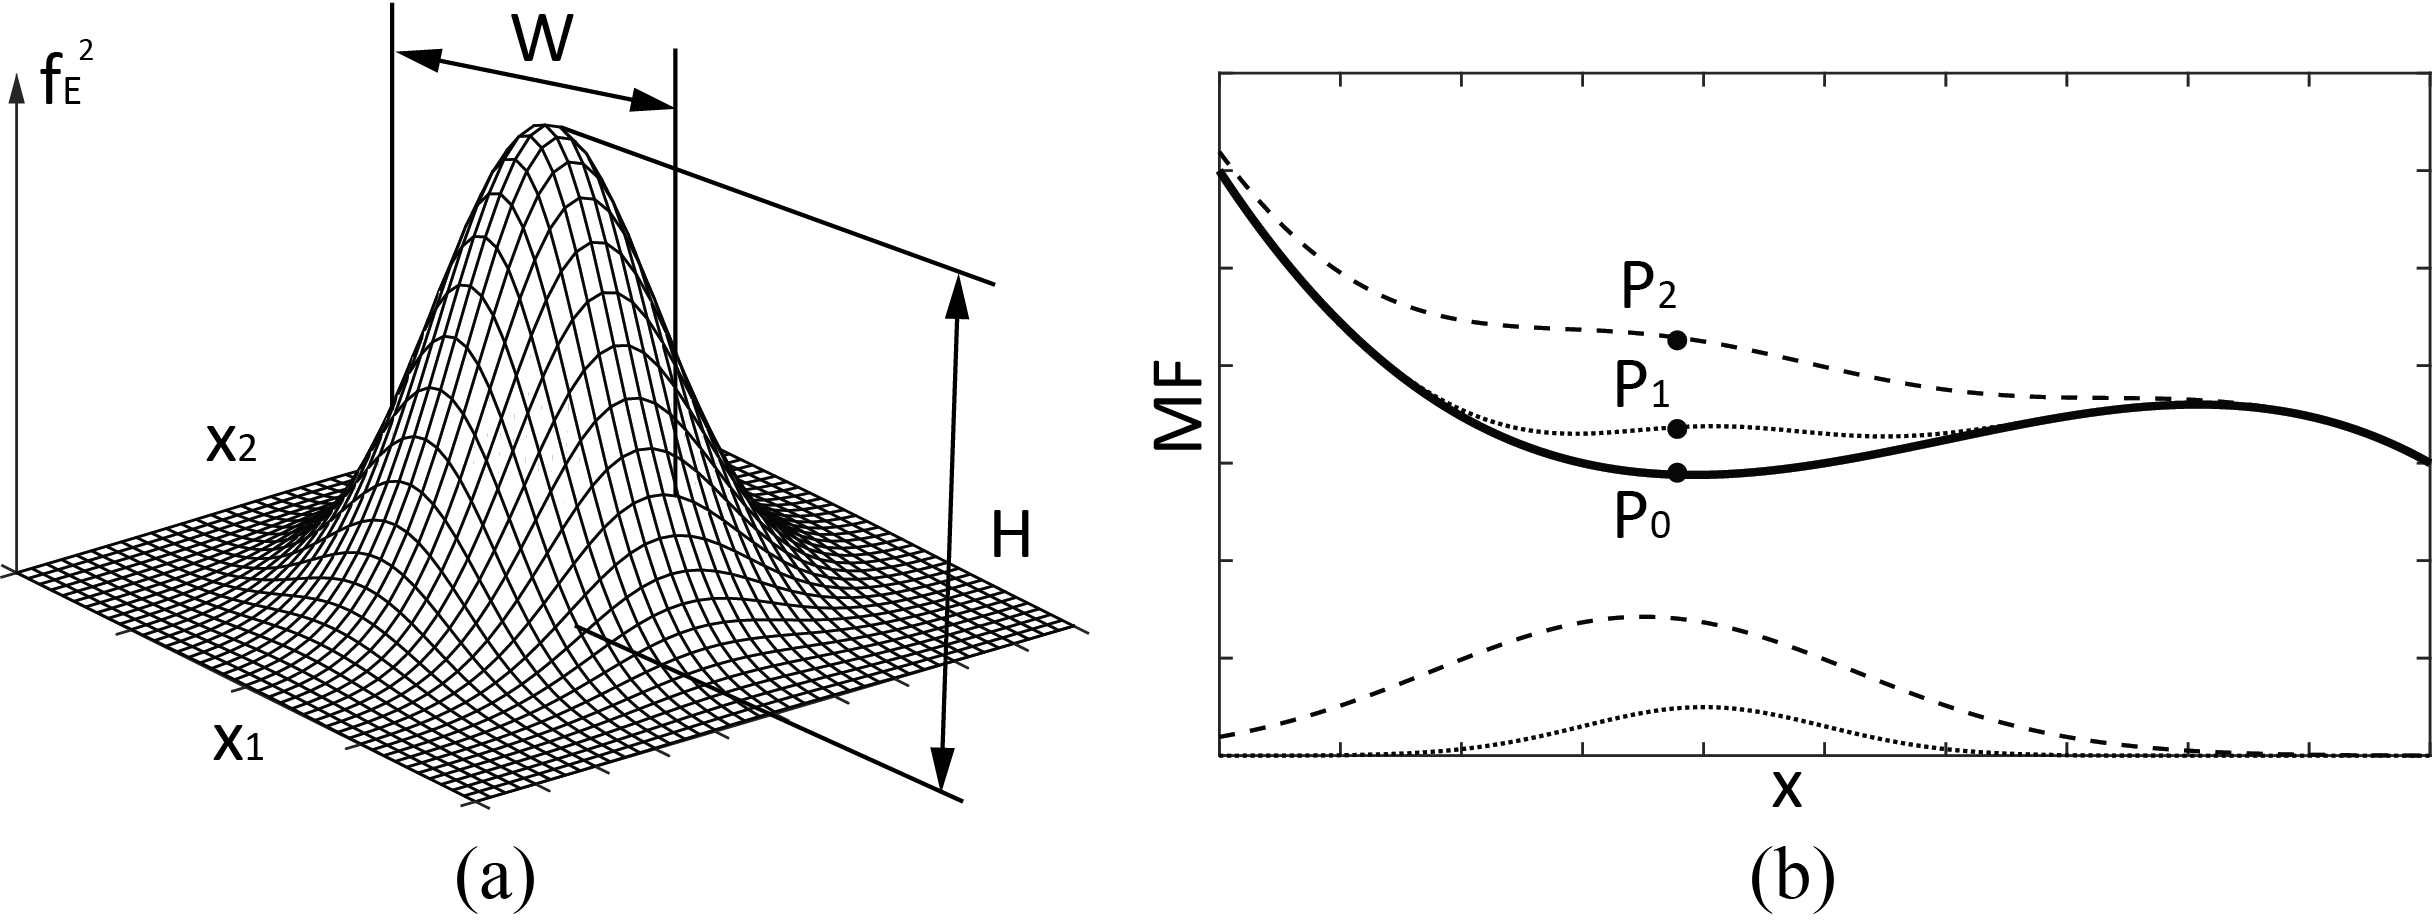
\includegraphics[scale=0.58]{chapter-1/figures/EscapeFunction_explained.png}
    \caption{Explanation of the method of escape function. (a) a 2-D escape function illustration, where $H$ modifies the height and $W$ modifies the width of the function. (b) $P_0$ is a minimum for the original 1-D merit function (solid line). By applying escape function (dotted line), $P_0$ is lifted to $P_1$. However, it cannot help the optimizer to escape to a new basin of attraction. When applying a different escape function (dashed line), $P_0$ is lifted to $P_2$. The optimizer escapes to the next basin of attraction.}
    \label{fig: Escape_function_explained}
\end{figure}
Figure \ref{fig: Escape_function_explained} -(b) uses a 1-D case to illustrate the escape function with two different settings. The solid line represents the original 1-D merit function. After local optimization routine, the minimum $P_0$ is obtained. In order to escape from the current basin of attraction, the first escape function setting lifts $P_0$ to $P_1$, as indicated by the dotted line. However, the optimizer remains in the same basin of attraction due to a insufficient modification of the local landscape. The second escape function setting lifts $P_0$ to $P_2$. When local optimization routine applied for $P_2$, the optimizer escapes from the original basin of attraction. In practice, an automatic feedback loop is designed to adjust the escape function settings to increase the efficiency for minimum searching \cite{Isshiki1998}.


\subsubsection{Generic algorithm}

The genetic algorithm is inspired by the process of natural selection which belongs to the larger class of evolutionary algorithm. Similar to biological reproduction, the genetic algorithm defines population in the optimization landscape. Crossover and mutation occur among the population through generations. The fitness of survival of a given individual is determined within the population. Individuals that have a high fitness will be selected by the algorithm.

In the context of optical design and optimization, the merit function value of an optical system configuration is equivalent to its fitness of survival. Solutions to optical systems are thought of as particular individuals of a hypothetical form of life \cite{Moore1999}. Variables can be compared to genes. The genes are represented by binary codes, which correspond to different variable values \cite{GAreview2018}. 

To initialize an optimization process by genetic algorithm, starting population is created in the optimization landscape. Two kinds of evolutionary activities are considered: crossover and mutation. Crossover happens when the genetic codes of the selected parents are exchanged. Mutation happens when the genetic codes randomly change for individuals. Multiple strategies for crossover and mutation are available. However, trial and error are often needed to determine these strategies. The exit criteria for the genetic algorithm is usually determined by the number of generation the population evolves. 

Different from the method of simulated annealing or escape function, genetic algorithm begins with sampling a larger range of the optimization landscape. Information in different part of the optimization landscape are exchanged to search for the global optimum. However, because of its combinatorial nature, the convergence to a minimum in the continuum variable space is not efficient. Hybrid algorithms where genetic algorithm combined with local optimizer (e.g. damped-least square) is thus recommended to improve the efficiency \cite{Moore1999}.

\textbf{Particle swarm optimization}
Particle swarm optimization was introduced as an analogue for the interaction of individuals in a swarm or a flock of birds. A collection of candidate solutions, called particles, move around in the optimization space according to simple mathematical rules. The goodness of a particle's location is given by the value of the merit function. For each particle, three vectors are used to represent it in the optimization space: the current location of the particle, the velocity of the particle , and its previous best position. During each iteration, every particle moves from its original location to a new location considering the velocity vector and the best location vectors.  After sufficient iterations, the swarm as a whole is likely to move close to an optimum in the optimization landscape \cite{MenkeParticleSwarm} . 

Similar to the genetic algorithm, particle swarm optimization starts with initializing a population randomly located in the optimization space. Each particle starts with an initial velocity. The position vector and velocity vector of the particles are updated after each iteration as the particles move. Parameters associated with the particle movement such as initial velocity, movement inertia, and acceleration with respect to the global best positions need to be determined based on trial and error. 

As for optical design, each system configuration represents a particle in the optimization space. Particle swarm optimization has been demonstrated in several design cases and it is especially helpful in handling large number of variables such as freeform systems \cite{MenkeParticleSwarm}. On the other hand, hybrid algorithm of combing particle swarm optimization with local optimizer has been proposed \cite{Guo:sParticleSwarm}: particle swarm optimization is used for the discrete optimization of the optical material choices, while the local optimizer is applied to obtain the minimum given the selected material choice.  

\textbf{Saddle point method}
In additional to minimum and maximum, saddle point is also a type of stationary points existing in the optimization landscape. Gradient vanishes at all stationary points. When computing the eigenvalues of the Hessian matrix of these stationary point, a minimum has its signs of the eigenvalues all positive, a maximum has its signs of the eigenvalues all negative, and the saddle point has both positive and negative signs of its eigenvalues. Morse Index is defined as the number of the negative signs of the eigenvalues, and the Morse Index of a saddle point is always bigger than \textit{1}. For example, if there is one negative eigenvalue of the Hessian matrix for a stationary point, it is then a saddle point with a Morse Index value of \textit{1}. For a \textit{N}-dimensional optimization landscape, the Morse Index value of its saddle points can vary from \textit{1} to \textit{N-1}.  The value of the Morse Index indicates the number of directions, following the eigenvectors, from which the merit function value decreases. An example of a saddle point in the \textit{2}-dimensional landscape is given in Figure \ref{fig: saddle_illustration} - (a). 

Figure \ref{fig: saddle_illustration} - (b) shows an example of a \textit{2}-dimensional landscape. If we use an analogue of a mountain view scenario, minima are the \textit{bottom} of the valleys and maxima are the \textit{top} of the hills. Saddle points are located on the passes between the valleys. 

\begin{figure}
    \centering
    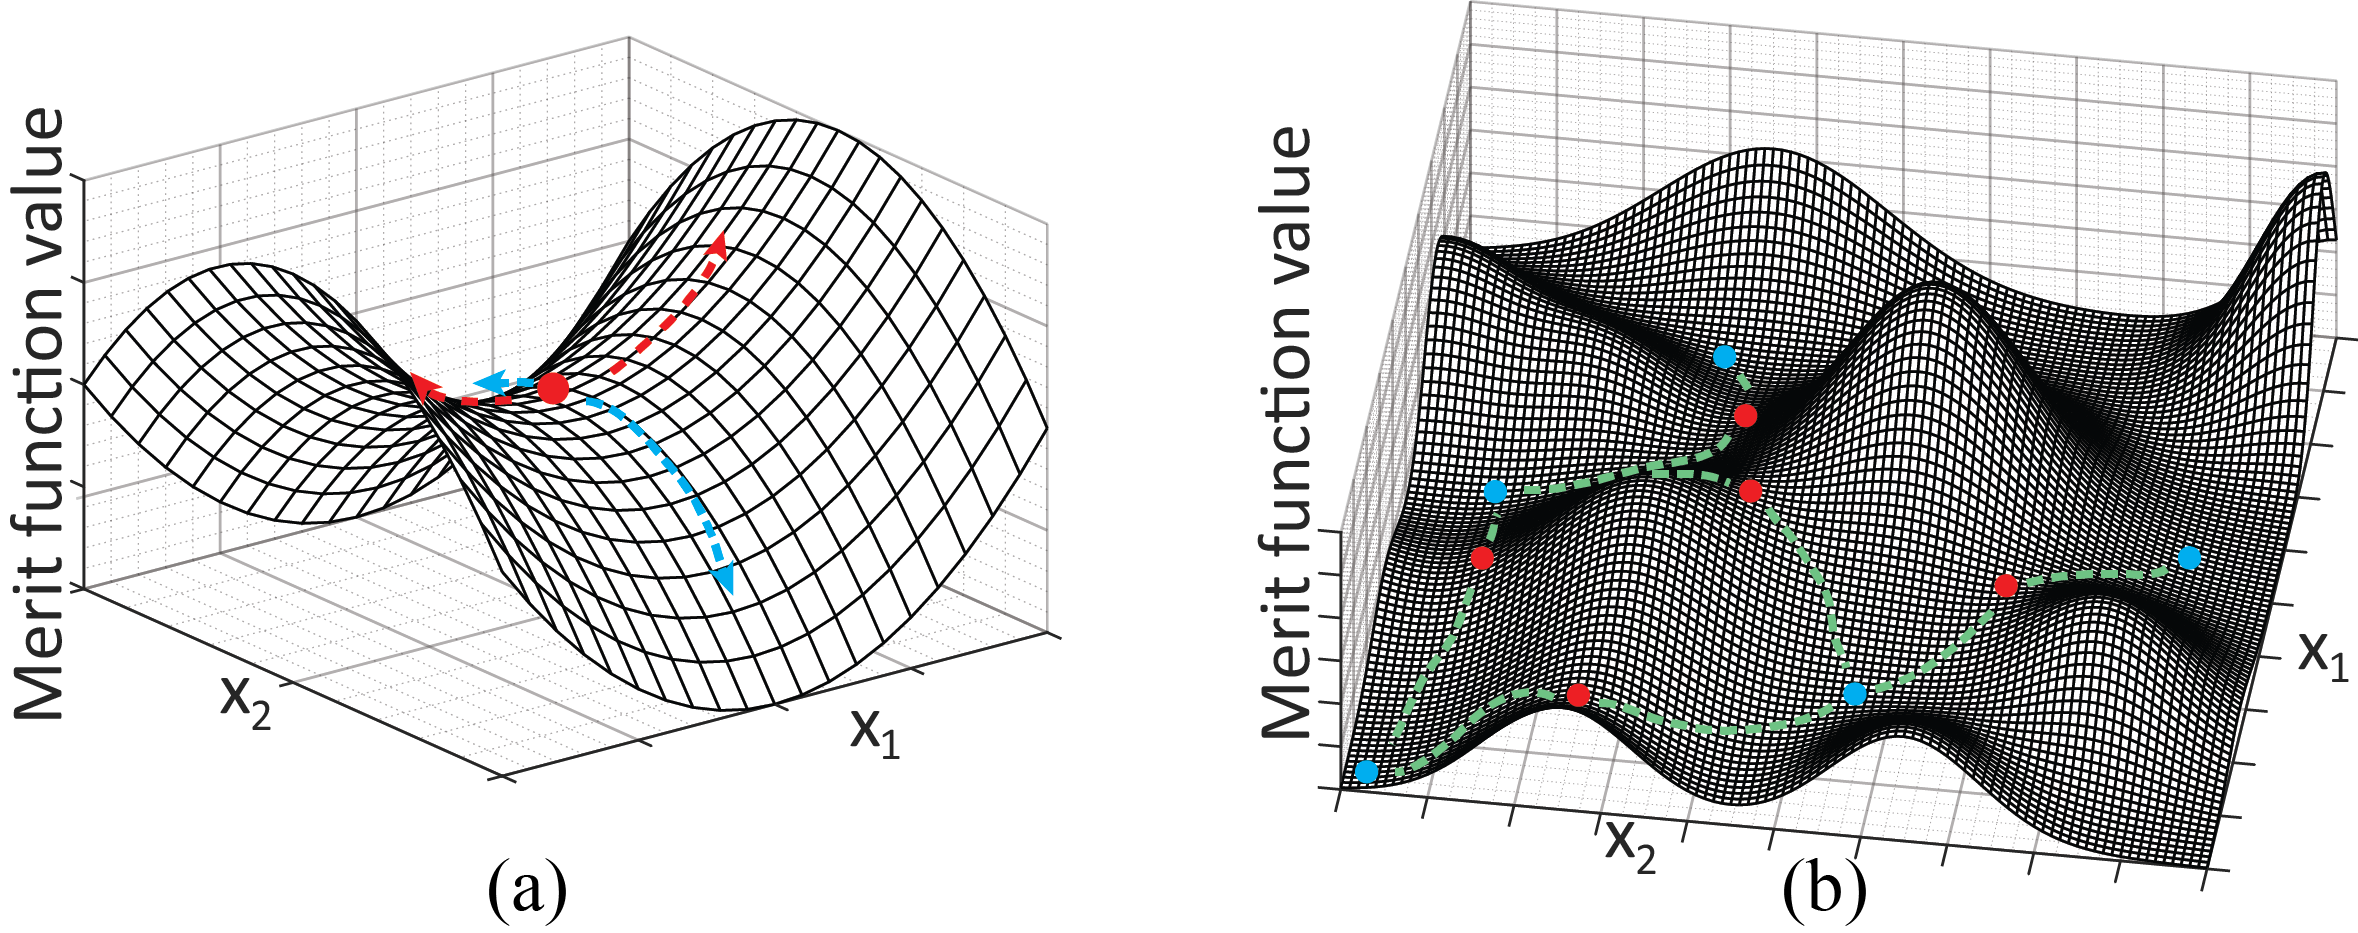
\includegraphics[scale=0.58]{chapter-1/figures/saddle_point_plotted.png}
    \caption{Illustration of the 2-D saddle points. (a) A 2-D saddle point (horse saddle, with a Morse Index value of 1). It s a maximum in one direction and a minimum along the other direction. (b) Example of a 2-D landscape where minima are connected via saddle points. }
    \label{fig: saddle_illustration}
\end{figure} 

The aforementioned global optimization methods treat the optimization landscape as difference basins of attraction. When a larger number of basins are covered, the chance of obtaining a global solution increases. Methods such as simulated annealing and escape function apply strategies to switch basins of attraction when a local minimum is encountered. Methods such as genetic algorithm and particle swarm start with a population distributed in the optimization space. Strategies were applied to search for the basin with the best fit minimum. As a result, the task of searching for local minima can be then replaced by the task of searching for basins of attraction. Saddle point is of special interest when the task is to search for different basins of attraction. As indicated in Figure \ref{fig: saddle_illustration}-b, saddle points with a Morse Index of \textit{1} are located at the boundaries between different basins. Once such a saddle point is found, two basins of attraction can be reached afterwards.

\subsubsection{Saddle point detection \label{method: spd}}

Network of Local Minima (NETMIN), a tool developed in Delft University of Technology, detects saddle points with Morse Index 1 in the optimization landscape. NETMIN uses constrained local minimization to search saddle points starting from a local minimum. As illustrated in Figure \ref{fig: spd_illustration}, a set of directions is defined around a local minimum. These directions can be determined by the eigenvectors of the Hessian matrix, which are computed at the local minimum. Around the local minimum, the surfaces along which the merit function is constant have the shape of ellipsoids \cite{MarinescuSPD07}. The eigenvectors of the Hessian matrix correspond to the directions of the half-axes of the ellipsoids. Along each direction, a set of hyperplanes which orthogonal to the direction vector can be defined. For $N$ -dimensional space, these hyperplanes have a dimension of $N-1$. The distance between the local minimum and the hyperplane is indicated by $t$. On each hyperplane, a constrained minimization can be performed. The positions of the constrained minima as a function of  $t$ is symbolically shown in Figure \ref{fig: spd_illustration} - (a). The merit function value ($MF$) as a function of $t$ is shown in Figure \ref{fig: spd_illustration} - (b). When $t$ is sufficiently small, the merit function value of the constrained minimum on the hyperplane increases. At a certain $t = t_{max}$, the merit function value reaches its maximum value (point $s$ in Figure \ref{fig: spd_illustration - (a)}). This point is a maximum along the vector direction and a minimum on the $N-1$ dimensional hyperplane, hence a saddle point with Morse Index 1.  

\begin{figure}
    \centering
    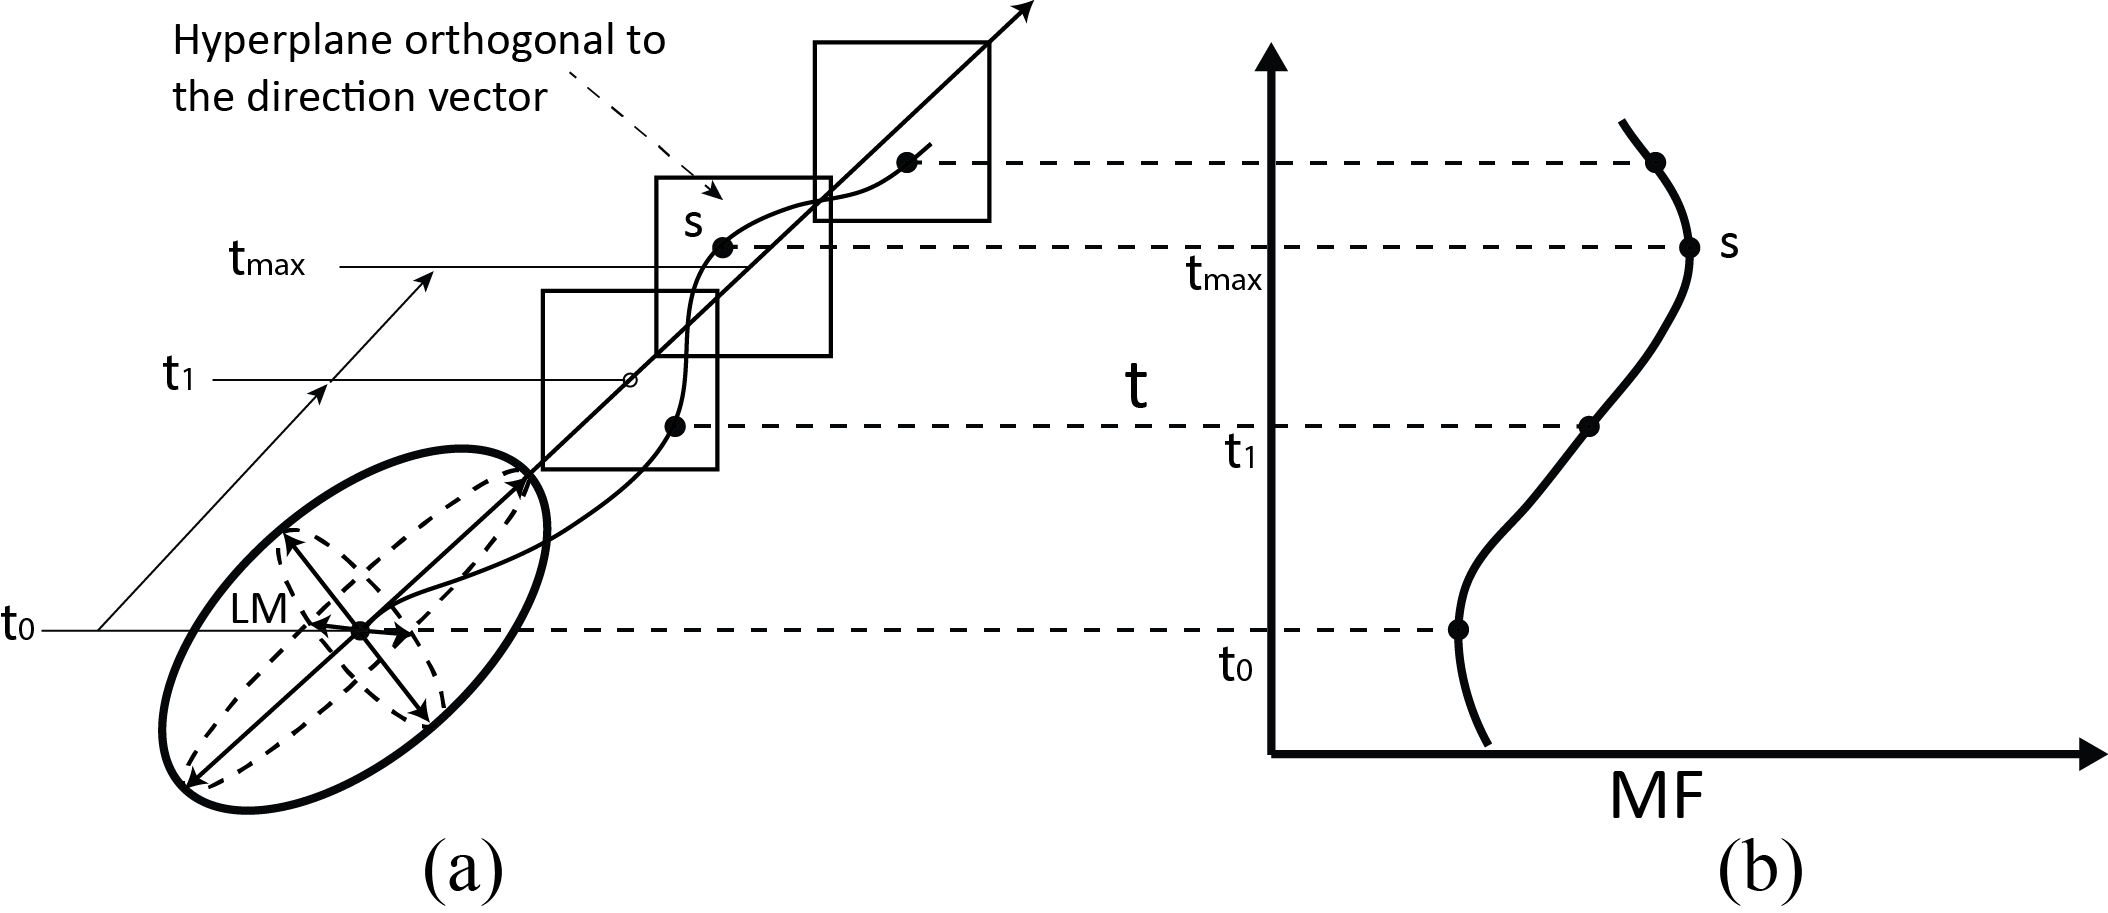
\includegraphics[scale=0.58]{chapter-1/figures/spd_plot.png}
    \caption{Illustration of constrained optimization to detect saddle point in the optimization landscape. (a) Saddle point detection in high-dimensional space. Minimization is performed on hyper-planes which are orthogonal to the chosen direction. (b) Example of MF value along a search direction. The saddle point detection starts from an existing local minimum. The directions around the local minimum are chosen towards the directions of the eigen vectors of the Hessian matrix. The value of the MF will first increase. After finding the saddle point, the MF value will decrease. }
    \label{fig: spd_illustration}
\end{figure} 

When a saddle point with Morse Index 1 is detected, a point "on the other side" of the saddle point can be chosen to start a local optimization routine. The optimizer searches in a different basin of attraction to find a new local minimum. NETMIN combines local optimizer and saddle point detection algorithm to reveal the network of local minima and saddle point in the optimization landscape. NETMIN has been used to study triplet network (\cite{PascalTriplet2009}) and six-mirror systems (\cite{MarinescuSPD07}). In Chapter 3 of this thesis, we also use NETMIN obtained results as a reference. 

The computation of NETMIN is expensive. For each step along the chosen direction, a constrained optimization has to be performed. In practice, multiple directions have to be searched to find all saddle points around a local minimum. Parallel processing can be enabled to facilitate the search.  


\subsubsection{Saddle point construction }
In the context of lens design, research has shown that saddle point can be constructed directly instead of performing a saddle point detection algorithm \cite{vanTurnhoutThesis2009} \cite{MVTurnhoutSPC15}. 

An illustration of the saddle point construction is given in Figure \ref{fig: spc_illustration}. The construction of a saddle point is indicated by step 1 and 2: It starts from a local minimum and adds an extra lens element to the existing system. When a saddle point system is obtained in step 2, step 3 and step 4 show how to obtain two new local minima from the saddle point system. The detailed explanation of saddle point construction is given in Chapter 2. 

\begin{figure}
    \centering
    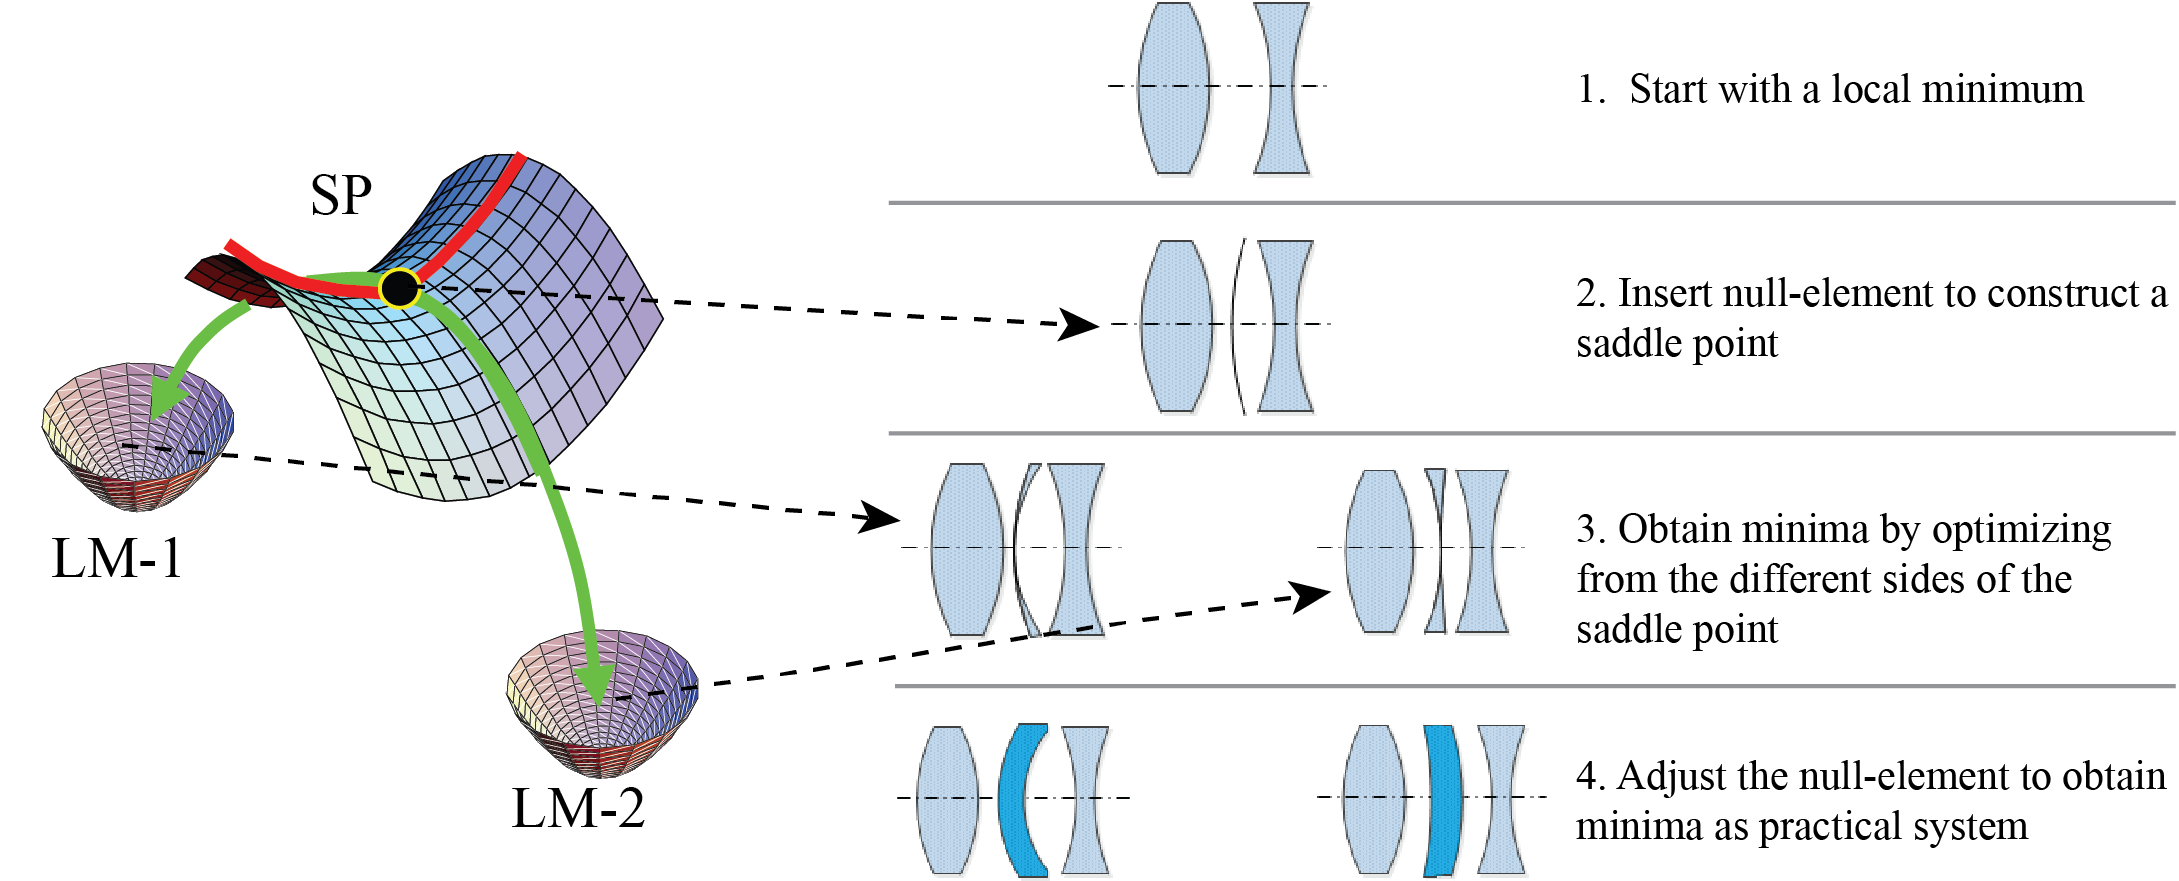
\includegraphics[scale=0.58]{chapter-1/figures/spc_illustrate.png}
    \caption{Illustration of the saddle point construction process. The right side shows an example of constructing a saddle point on a doublet minimum. Two triplet minima result from this process. The left is an example of how a saddle point leads to two minima in a 2D optimization space. In step 2 and 3, the optimization space remains static. In step 1 and 2, the optimization space has different dimensions (step 1 does not include the null-element, and step 4 adds extra variables). }
    \label{fig: spc_illustration}
\end{figure} 

% the next chapter is dedicated to saddle point construction. In this part, it is sufficient to introduce the topic.

% what is added research value of this thesis

%%%%%%%%%%%%%%%%%%%%%%%%%% SECTION 5 %%%%%%%%%%%%%%%%%%%%%%%%%%%%%%%%%%%%%%%%%%%%%%%%%%%%%%%%
\section{Goal and outline of this thesis}
As stated, one of the major challenge in optical design is to obtain a good solution among many sub-optimal solutions. The conventional way requires years of design practices. The designer has to accumulated enough experience to get in-depth knowledge in optical design, in order to master different type \footnote{The type refers to different optical systems such as photographic system, microscopic system, or telescopic system etc.. Different application has different requirements which result different type of systems.} of optical system design and navigate through different solutions. The late optimization technique requires less knowledge about the optical system and searches for the design landscape automatically. However, trial and error is still needed to set the optimization configuration parameter. The process also excludes the designer from the intermediate steps, and directly provides results. It requires constraints for the optimization to be carefully set to prevent unwanted solutions.   

SPC can rapidly obtain design solutions in lens design problems, regardless of the system types. The new solutions are obtained based on a unique property in the lens design landscape: saddle points can be constructed from existing local minima by adding extra variables. From the constructed saddle points, new solutions can be obtained. This provides a systematic way of getting solutions in design landscape. In relative simple design landscapes (e.g. triplet), the design solutions are observed to be connected via a network formed by saddle points and minima \cite{PascalTriplet2009}. It indicates a possibility, given the solutions are all connected via saddle points which can be constructed, that starting from any minimum in this network, most avaialble solutions can be systematically found. Therefore, the global optimal solution can also be found. Based on the properties of the SPC, in \colorbox{orange}{Chapter 2}, we give recommendations on how to use the SPC method in practice to obtain solutions in a lens design problem.

In a piratical design problem, the design landscape is never static. Constraints and general system specifications (e.g. EFL, field of view etc.) are constantly adjusted during the design process. It results a design landscape that also changes. In \colorbox{orange}{Chapter 3}, we show that in a wide angle pin-hole triplet network, how the network of minima and saddle points can change when system specification changes. For example, minima found in a previous status of the landscape can merge with a saddle point in a new status. 

\colorbox{orange}{Chapter 2} gives recommendation to apply SPC when an inserting position is given. However, there is still lack of insight regarding the determination of the inserting position. Brutal force can be used to try out every possible positions, but in a later stage of the design, the designer may not want to get a system with very different characteristics. \colorbox{orange}{Chapter 4} demonstrates some examples where SPC is applied to lens systems with increased complexity: a six-element wide angle lens, a microscopic objective and a lithorgraphic objective. Combined with expert insight on inserting position, the effectiveness of SPC providing new solutions is proven. 

In \colorbox{orange}{Chapter 5}, instead of conventional spherical lens design, we extend our exploration to the design landscape of aspheric systems. SMS method and different optimization strategy for aspherising the lens surface are compared. Finally, the conclusion of the main chapters are summarized in \colorbox{orange}{Chapter 6}.
\references{dissertation}

\begin{comment}

%%%{BACK-UPS
\subsection{Backup notes}
where to insert the lens -> combine with experience 
whether the result is satisfactory -> judge by experience 
controlled way of the getting the solution 

Neural network? 
It is a hot topic so it is good to also mention something about the Neural network work. 
\cite{JM_nn_93}  \cite{Yang:19} \cite{Cote:19}

\section{Problem for optical system design}

When designing an optical system, it is always necessary to consider its source and receiver. When designing imaging system, the object represents the source, where lights from all angles are emitting from the object at each point. The receiver is usually called image, which is normally a flat plane (such as a photosensitive film, or a charged-carrier device sensor). The optical system is located between the source and receiver, after which the light will arrive at the receiver with a designed performance instead of propagate in the air. The source and receiver in a non-imaging system can have more variety: a source can be a simple point source, or can be an extended source with a certain geometrical shape. The receiver can be all kinds of 3D-shape. 

An optical design problem uses all the available components which manipulate the light in a way that it will achieve a certain purpose as the designer desired. This can be either imaging, to focus a point in the object side to the image side with the maximal retained information, or can be non-imaging, to distribute the energy of the light in a way for a certain purpose, such as creating a homogeneous illumination. 

When mentioning optical design, the term is not specified enough. It should be including all the possible way of designing with manipulating light to achieve certain purpose. Regardless of the using of the components or the scale of the components. 

Optical design components, polarizer, diffractive components, multiple aperture (light field camera, cell-phone camera).

The design case mainly handled in this thesis is the imaging system design, in particular with optical lens design. In this case, the used components are mainly 

\end{comment}



\chapter{The Saddle Point Construction Method}
\label{chapter_2}
\graphicspath{ {./chapter-sp/figures/} }
\captionsetup[figure]{labelfont=bf}
\captionsetup{margin=1.5em}
\captionsetup[table]{labelfont=bf}
%% The following annotation is customary for chapter which have already been
%% published as a paper.


%% It is only necessary to list the authors if multiple people contributed
%% significantly to the chapter.
%\authors{Albert {\titleshape Einstein}}

%% The '0pt' option ensures that no extra vertical space follows this epigraph,
%% since there is another epigraph after it.

\begin{abstract}
The saddle point construction method is elaborated in this chapter. Recommendations on how to apply the method are given based on simple examples.
\end{abstract}

%% Start the actual chapter on a new page.
\newpage

\noindent 
The saddle point construction (SPC) method is one of the major methods investigated in this research. Several variations of the methods for constructing the saddle point system have been introduced through the years \cite{BociortSPCSexplained}\cite{MVTurnhoutSPC15}\cite{HouProc2015}. Instead of searching for alternative local minima, the SPC method constructs saddle points as intermediate steps to obtain new local minima. This is achieved by adding extra variables to the existing system. With this approach, it is shown in this chapter that it is possible to obtain new solutions in a systematic way. 

%%%%%%%%%%%%%%%%%%%%%%%%%%%%%%%%%%%%%%%%%%%%%%% Section SPC %%%%%%%%%%%%%%%%%%%%%%%%%%%%%%%%%%%%%%%%%%%%%
\section{Saddle point and design landscape}
For a given optical design problem, once the merit function and the number of variables N have been determined, an N-dimensional design (optimization) space is defined. The optimization of an optical system then is equivalent to finding the minimum of the merit function in the N-dimensional design landscape. As mentioned in the introduction, the optimization problem of optical design is a nonlinear problem, where multiple local minima are present in the design landscape. As a result, searching for one or several good local minima among many becomes a challenge for optical design. 

For the simple case of only two variables, the minima can be viewed as the bottoms of the valleys in the design landscape. On the other hand, maxima are the mountain tops, which are usually not observed in the lens design landscape. Minima and maxima are both critical points. A critical point is a point where the gradient of the merit function equals zero. In addition to minima and maxima, there are saddle points, which are also critical points and can be used to find new local minima.

In a two dimensional space, a 2-D saddle point is a "saddle" where along one direction in variable space, the value of the function decreases with respect to the saddle point value, while along the perpendicular direction, it increases. Mathematically, the so-called Morse Index is used to distinguish minima, maxima and saddle points. The Morse Index is defined as the number of negative eigenvalues of the Hessian matrix \textbf{$H$} at the critical point, when the Hessian matrix \textbf{$H$} is non-degenerate. A negative eigenvalue indicates that along the direction defined by the corresponding eigenvector of the Hessian matrix, the critical point is a maximum. Therefore, in an N-dimensional space, the Morse Index of a minimum and a maximum is 0 and N respectively. A saddle point can have any Morse Index between 1 and N-1. 

In this research, the saddle point with a Morse Index of 1 is of particular interest. This kind of saddle point has one direction, along which the value of the merit function decreases, while in N-1 other directions the merit function increases. This means that a saddle point of Morse Index 1 is a local minimum in all but one direction. When the optimization follows the two opposite directions in which the merit function descends, two local minima can in principle be found (Figure \ref{fig:SPCdemo}-b). As a result, if there is a way to rapidly obtain these saddle points in the design landscape, it provides an approach to find more local minima. In fact one finds two local minima from a saddle point of Morse Index 1. 

\section{The Saddle Point Construction method}
In this section, the SPC method and its variations are introduced and explained. As the name suggests, the method constructs saddle points in the design landscape. These are all saddle points with Morse Indices of $1$  \footnote{In the special version of the SPC, it can be proven that the Morse Index of the constructed saddle point is $1$. In the general version of the SPC, it is shown in the numerical experiments that the Morse Index of the constructed saddle point is $1$}. Instead of optimizing from an arbitrary point in the landscape, optimizing from a saddle point can systematically lead to two local minima. 

The saddle points are constructed by adding extra variables to the merit function that has attained the existing local minimum using the original number of variables. In principle, the variables can be any parameter in the lens design model. It should be mentioned that the most effective variables that have been used so far are the lens curvatures. 

\subsection{The general version of Saddle Point Construction \label{spc-general}}
\label{SPC_general}
The SPC method always starts with an optimized lens system that is a minimum of a merit function defined by N arbitrary variables. A saddle point then can be constructed in a design space with $N + 2$ variables by adding a lens with zero thickness and with surfaces having the same curvatures (see Figure \ref{fig:SPCdemo}(a)). Such a lens has no optical effect and hence the merit function is the same after insertion of this element as before. The two curvatures are the two new variables, so that the total number of variables has been increased to N+2. For certain values of the curvatures of the inserted surfaces, the resulting system is a saddle point, which is a minimum along $N + 1$ directions in the variable space and a maximum along one direction (i.e., mathematically it will have a Morse index of 1 \cite{MVTurnhoutSPC15}). The details of how such values are obtained will be explained in the part later. Along the direction for which the SP is a maximum, two minima can be obtained systematically, as shown for simplicity in a 2D case in Figure \ref{fig:SPCdemo}(b).

\begin{figure}[h!]
    \centering
    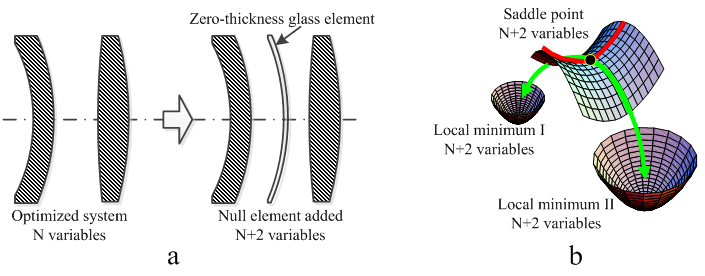
\includegraphics[scale=0.68]{chapter-2/figures/FigSPCDemo.png}
    \caption{Illustration of the SPC. (a) An SP in N+2 dimensional space obtained by insertion of a zero-thickness glass meniscus. (b) A Morse index 1 saddle point in the 2D case.}
    \label{fig:SPCdemo}
\end{figure}

The pair of surfaces with equal curvatures can be either a zero-thickness lens added to the original minimum or a zero-thickness air space inside a lens. Both the added lens and the added air space with zero thickness, do not affect the ray paths, and hence the merit function value of the original system is not changed. Such an element of zero thickness is therefore called a null element. 
Given the merit function $MF$ at a local minimum in $N$ dimensional space
\begin{equation}
MF^{N}(x^{0}_1, x^{0}_{2},...,x^{0}_{N}),
\end{equation}we have 
\begin{equation}\label{eq_mflm}
\frac{\partial}{\partial{x_i}}MF^{N}(x^{0}_1, x^{0}_{2},...,x^{0}_{N}) = 0, \;\; \text{for} \; i =1,2,...,N.
\end{equation}Furthermore the Morse Index of the Hessian at $(x^{0}_1, x^{0}_{2},...,x^{0}_{N})$ is zero, i.e. the eigenvalues of the matrix
\begin{equation}
H^{N}_{ij}=\frac{\partial^2}{\partial{x_i}\partial{x_j}} MF^{N}(x^{0}_1, x^{0}_{2},...,x^{0}_{N}),
\end{equation}are all non-negative.

Next we introduce a null element with common curvature $c_1=c_2$ of its two surfaces. Additional variables are then introduced as follows:

\begin{equation}
\begin{align}
\begin{rcases*}
x_{N+1} &= c_1 + c_2, \;\;\\
x_{N+2} &= c_1 - c_2. \;\;
\end{rcases*}
\end{align}
\end{equation}

Because the introduction of the null-element does not alter the physical property of the optical system, therefore does not have any effect on the merit function, we have the following relation between the $N$ and $N+2$ dimensional merit functions:
\begin{equation} \label{eq_mfconst}
MF^{N+2}(x_1, x_{2},...,x_{N}, x_{N+1},x_{N+2}=0) = MF^{N}(x_1, x_{2},...,x_{N}).
\end{equation}%because the variables are introduced in a way that the physical property of the optical system is not altered with the null-element. Therefore, the value of the merit function stays constant. 
%for some $(x_1, x_{2},...,x_{N-2})$ in some (sufficiently small) neighbourhood of  $(x^{0}_1, x^{0}_{2},...,x^{0}_{N-2})$ and all $x_{N-1}$. 
%Equation \ref{eq_mfconst} together with Equation \ref{eq_mflm} implies

Equation \ref{eq_mflm} implies
\begin{equation}
\begin{split}
\frac{\partial}{\partial{x_j}}MF^{N+2}&(x^{0}_1, x^{0}_{2},...,x^{0}_{N},x_{N+1},x_{N+2}=0) \\
&= \frac{\partial}{\partial{x_j}}MF^{N}(x^{0}_1, x^{0}_{2},...,x^{0}_{N}) \\
&= 0, \\
\text{for all} \: &j = 1, 2, ..., N, \:\: \text{and all} \:\: x_{N+1}.
\end{split}
\end{equation}Furthermore Equation \ref{eq_mfconst} implies 
\begin{equation}\label{MF_xn-1_fozero}
\frac{\partial}{\partial{x_{N+1}}}MF^{N+2}(x_1, x_{2},\cdots,x_{N}, x_{N+1},x_{N+2}=0) = 0,
\end{equation}%for all $(x_1, x_{2},...,x_{N-2})$ in a neighbourhood of $(x^{0}_1, x^{0}_{2},\cdots,x^{0}_{N-2})$ and 
for all $x_{N+1}$. 
Equation \ref{MF_xn-1_fozero} applies to $(x^{0}_1, x^{0}_{2},...,x^{0}_{N})$, we have
\begin{equation}
\begin{split}
\frac{\partial}{\partial{x_{N+1}}}MF^{N+2}&(x^0_1, x^0_{2},...,x^0_{N}, x_{N+1},x_{N+2}=0) = 0,\\
&\text{for all}\; x_{N+1}.
\end{split}
\end{equation}Next we vary $x_{N+1}$ to find a point $x^0_{N+1}$ for which 
\begin{equation}\label{eq:1dsearch}
\frac{\partial}{\partial{x_{N+2}}}MF^{N+2}(x^0_1, x^0_{2}, \cdots,x^0_{N}, x^0_{N+1},x_{N+2}=0) = 0.
\end{equation}Assuming that such point $x^0_{N+1}$ can be found, we conclude that 
\newline

\centerline{$(x^0_1, x^0_{2},\cdots,x^0_{N}, x^0_{N+1},0)$} 
\newline \noindent is a critical point of $MF^{N+2}$. 
 
Now Equation \ref{eq_mfconst} implies
\begin{equation}
\begin{split}
\frac{\partial}{\partial{x_i}\partial{x_j}}MF^{N+2}&(x^{0}_1, x^{0}_{2},...,x^{0}_{N},x^{0}_{N+1},x_{N+2}=0) \\
&= \frac{\partial}{\partial{x_i}\partial{x_j}}MF^{N}(x^{0}_1, x^{0}_{2},...,x^{0}_{N}), \\
\text{for} \;\;&\; 1\leq i,j \leq N.
\end{split}
\end{equation}Furthermore, from Equation \ref{MF_xn-1_fozero}
\begin{equation}
\begin{split}
\frac{\partial}{\partial{x_i}\partial{x_{N+1}}}MF^{N+2}&(x^{0}_1, x^{0}_{2},...,x^{0}_{N},x^{0}_{N+1},x_{N+2}=0) = 0, \;\; \\
\text{for all} & \;1\leq i \leq N+1.
\end{split}
\end{equation}
So we have for the Hessian in \textit{N+2} dimensional space
\begin{equation}\label{eq: the hessian}
\left( H^{N+2}_{ij} \right) = 
\begin{bmatrix}
\Large{\left( H^N_{ij} \right)}       &                 &   0                  & \frac{\partial{^2MF^{N+2}}}{\partial{x_1}\partial{x_{N+2}}} \\[2em]
                                                    &                 & \vdots         & \vdots \\[2em]
 0                                                 & \cdots    & 0                  & \frac{\partial{^2MF^{N+2}}}{\partial{x_{N+1}\partial{x_{N+2}}}}  \\[2em]
 \frac{\partial{^2MF^{N+2}}}{\partial{x_{N+2}}\partial{x_1}}   &\cdots  & \frac{\partial{^2MF^{N+2}}}{\partial{x_{N+2}}\partial{x_{N+1}}} & \frac{\partial{^2MF^{N+2}}}{\partial{x^2_{N+2}}}
\end{bmatrix}.
\end{equation}The last column and last row are in general nonzero, hence there are in general nonzero eigenvalues.
The eigenvalues of $H^{N}_{ij}$ are similar to a subset of $N$ eigenvalues of $H^{N+2}_{ij}$, but they are not the same. Nevertheless, it may be expected that they have the same sign, i.e. they are positive for

\vspace{0.1em}
\centerline {$(x^0_1, x^0_{2},\cdots,x^0_{N}, x^0_{N+1},0)$.}
\vspace{0.5em}

The question still remains what the sign is of the remaining two eigenvalues, because these signs determine the Morse Index at point $(x^{0}_1, x^{0}_{2},...,x^{0}_{N},x^{0}_{N+1},0)$.
\vspace{0.3em}

In practice, what has been observed so far in the SPC is that there are one positive sign and one negative sign. That means the point is a saddle point with Morse Index value of $1$. 

Obtaining saddle point systems with the general version of the SPC includes the following steps:
\begin{enumerate}[nosep] \label{para: performing SPC scan}
\item Insert a null element into the existing minimum.
\item Compute the derivative (numerically) of the merit function with respect to the curvature of the inserted null element. The null element has two identical curvatures. The computed derivative of the two curvatures have opposite sign. 
\item Select the curvature values where the derivative of the merit function equals zero. Systems with these curvature values are the saddle point systems. 
\end{enumerate}
These steps are referred as "performing an SPC scan" in this thesis.  In our research, the SPC scans are performed in CODE V using the MACRO function. Figure \ref{fig:SPCscan} shows an example of the results of such an SPC scan. An SPC scan in a chosen position can lead to multiple saddle point systems.  There are four zero crossings in Figure \ref{fig:SPCscan}(b) indicating that four saddle points are found. When the saddle points are found, initial systems for subsequent local optimization can be obtained by choosing for each zero crossing in Figure \ref{fig:SPCscan}(b) two systems, one to the left, one to the right of the saddle point. Local optimization, using, e.g., a damped-least square (DLS) algorithm, will then lead to two minima, one on each side of the “saddle,” as shown in Fig \ref{fig:SPCdemo}(b). To obtain the broadest variety of new minima with SPC, in general both zero-thickness lenses and zero-thickness air spaces are necessary. For simple systems, there are examples of minima that can be obtained with one of these two types of null elements but not with the other one. Finding the saddle points is in principle much less time consuming than DLS optimization, because it only involves the evaluation of the derivative of the MF for the 1D sequence of scan points according to Equation \ref{eq:1dsearch}, whereas local optimization involves many iterations where a Jacobian matrix is evaluated. The zero-thickness condition for the null element is not a severe limitation, as it may seem, because in the resulting minima the distances between the surfaces (and the glass of the new lens) can be easily changed as desired. Once the two local minima are obtained with the SPC, other parameters of the new lens (thickness, aspheric coefficients, etc.) can be made available as variables to further minimize the merit function.

\begin{figure}[h!]
    \centering
    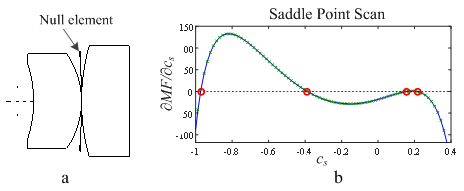
\includegraphics[scale=0.8]{chapter-2/figures/SPCscan.png}
    \caption{Example of an SPC scan. (a) The insertion of a glass null element between two lenses exhibiting a known minimum value of the merit function. (b) The SPC scan finds four saddle points in this search. The red circles indicate the corresponding values of the null element curvatures.}
    \label{fig:SPCscan}
\end{figure}

\subsection{The special version of Saddle Point Construction}
\label{SPC_Special}
Different from performing a scan using the general version of the SPC, the special version of the SPC directly constructs the saddle points by adding null elements to the existing system. This kind of null element (a glass or an air element) has to be attached to one of the existing surfaces in the system. The two curvatures of the null element have to be the same as that of the surface in contact. In such a case, three surfaces have the same curvatures and two zero-thickness spaces between them as illustrated in Figure \ref{fig:SPCS-illus}. It is explained in the previous section that such a constructed system can be a saddle point system with a Morse Index of either $1$ or $2$ (one negative eigenvalues or two negative eigenvalues from the remaining two for the Hessian matrix shown in Equation \ref{eq: the hessian}). In practice, we have not observed any case with a Morse Index of $2$ in our numerical experiment. When an equality constraint \footnote{For an optimization problem $min f(\mathbf{x})$, an equality constraint means that the problem is subject to $g_{equa}(\mathbf{x})=C_1$. An example of an inequality constraint can be that the problem is subject to $g_{inequa}(\mathbf{x}) > C_2$.} (e.g. a constraint on effective focal length) is applied to the system, it can be proven that such a saddle point system has a Morse Index of $1$ \cite{BociortSPCSexplained}.

\begin{figure}[h!]
    \centering
    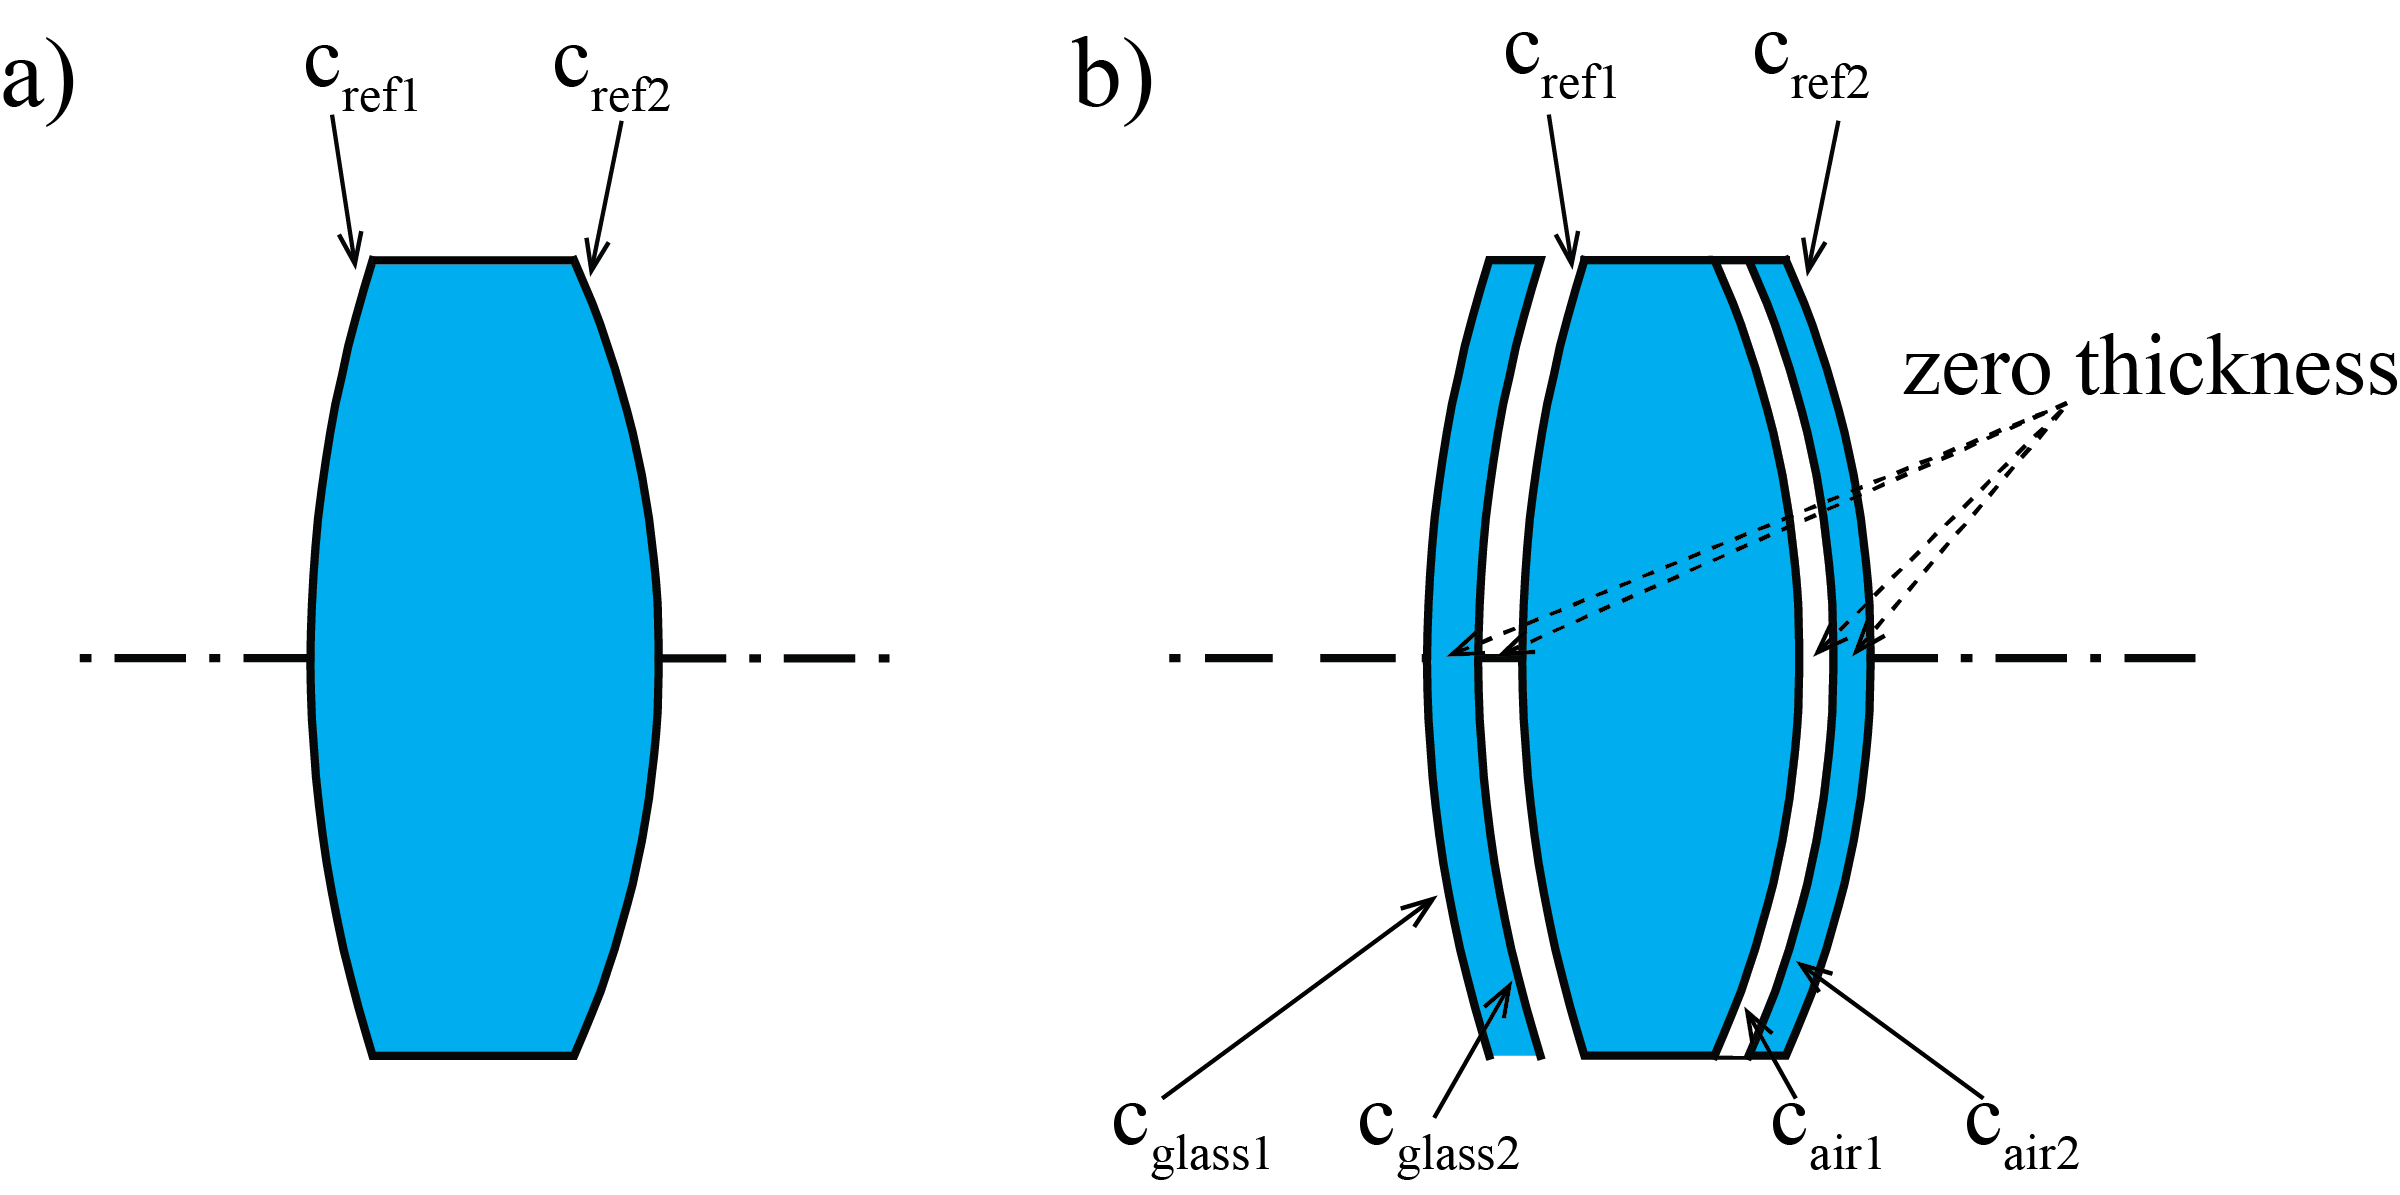
\includegraphics[scale=0.45]{chapter-2/figures/SPCS_illus.png}
    \caption{Illustration of the special version of SPC. a) A lens before adding any null element. b)  A glass null element has been attached to the surface on the left. An air null-element has been attached to the surface on the right. $c_{glass1} = c_{glass2} = c_{ref1}, c_{air1} = c_{air2} = c_{ref2}$. The speical version of the SPC usually adds one glass null element or one air null element. For demonstration purpose, different types of null elements are added to the lens, and the thickness of the null elements are also added.}
    \label{fig:SPCS-illus}
\end{figure}

Compared to the general version of the SPC, the special version is a rapid way to construct saddle point systems. However, the constructing positions are limited to the locations of the existing surfaces. As a result, some of the saddle points found by the general version can not be obtained by the special version of the SPC. In this research, the general version of the SPC is mainly used for acquiring new minima. When an SPC scan is performed on an existing surface, the saddle point constructed by the special version of the SPC can also be obtained. 

%%%%%%%%%%%%%%%\subsection{Saddle point construction intermediate}%%%%%%u%%%%%%%%

\section{Recommendations for applying Saddle Point Construction}\label{section: SPC recommendation}
As mentioned in the previous section, the SPC adds two extra curvatures to an existing optical system. It is straight forward, if the design goal is to add new elements to the system. Nevertheless, when applying the SPC in the practical design scenario, the technique can be used in different ways to achieve different design goals. Some scenarios are listed below as recommendations.

\subsection{Adding lens elements}
The direct way of applying SPC is to add a lens element to the existing system. This can be achieved by either inserting a glass null element or an air null element. Essentially, both approaches introduce two curvature variables to the system. Adding a glass null element can be treated as adding a lens element, while adding an air null element can be regarded as splitting an existing lens. The two approaches are described in the following two paragraphs.

\subsubsection{glass null element - adding a lens}
The Cooke triplet is chosen here as an example to demonstrate how SPC is applied. 
The position of the insertion of the glass null element is indicated by the dashed line in Figure \ref{fig:SPC-glass null element}. In principle, any position in the spaces between the lenses can be selected for the insertion. The choice of the position can be guided by the conventional lens design method. Examples of combining a traditional design method and the SPC method are given in Chapter 4.

In Figure \ref{fig:SPC-glass null element}, the insertion position is chosen between the middle lens and the right lens. As shown in the SPC scan curve, three zero-crossing points of the derivative of the merit function are found, hence three saddle points are found. Three new solutions with the added lens are listed in the same figure. Based on the scan curve, one would expect four solutions instead of three to be produced after optimizing from the three saddle points. It is the case when the minima are in the form of having an element with zero-thickness. However, when the thickness of the inserted element is increased, solution will disappear or merge with other solutions (an example is given in the next chapter in Figure \ref{fig:thicknesschange}). This is the situation in this example, and only three minima remained once the thickness is increased to a practical value. Among the three solutions, the added lenses present different optical powers. The original lens elements of the system remain almost the same powers compared to the status before insertion. In this example, two systems have better MF values (left system MF 43.27 $\mu m^2$, right system MF 47.80 $\mu m^2$) than the original one (MF 49.95 $\mu m^2$). The merit function used here is the default transverse-ray function in CODE V. It is a composite value, scaled so that it is the mean square of the weighted image radius.

\begin{figure}[h!]
    \centering
    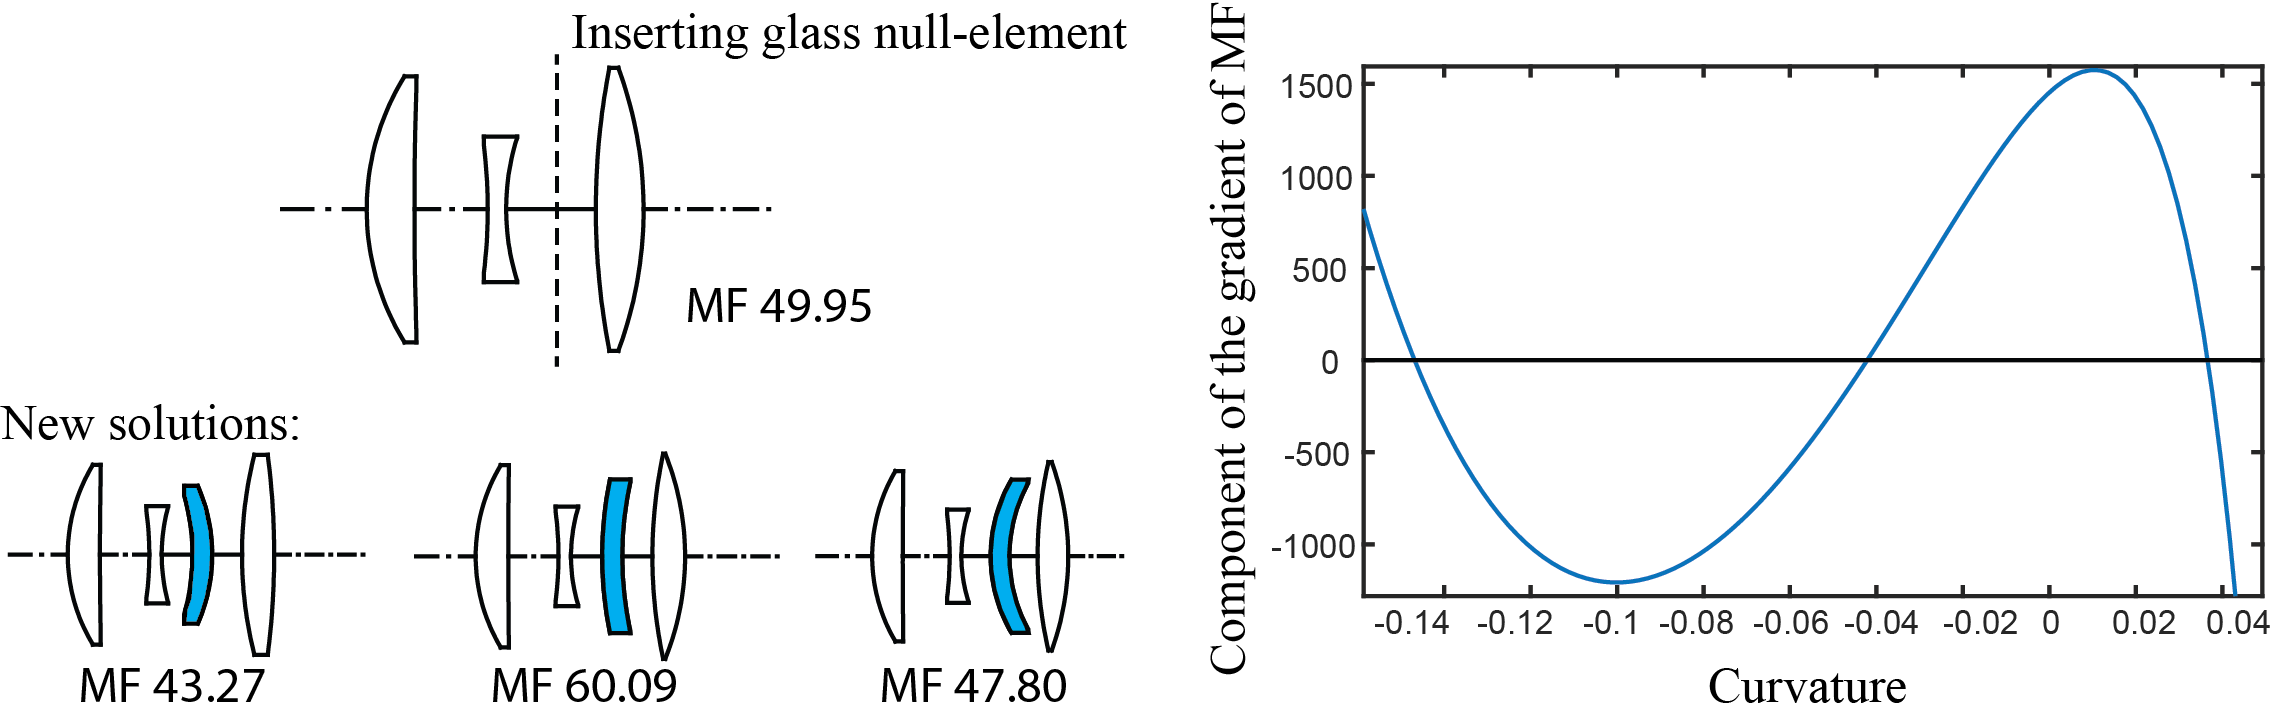
\includegraphics[scale=0.68]{chapter-2/figures/spc_add_glass.png}
    \caption{Adding lens element by adding glass null element using the SPC. The dashed line indicates the position where the null element is inserted. Three saddle points lead to four solutions with zero-thickness element (not shown). When the thickness of the inserted element is increased, three solutions with one lens more are obtained. The added lens elements are highlighted. MF values are listed for each system, and the unit is $\mu m^2$. }
    \label{fig:SPC-glass null element}
\end{figure}

\subsubsection{air null element- splitting a lens}

Alternatively, adding lenses can also be realized by splitting lenses. With the SPC, inserting an air null element into a lens is equivalent to splitting this lens. In Figure \ref{fig:SPC-air null element}, the most right lens element was chosen to be split. The dashed line indicates where the lens was split. The derivative as function of the curvature of the inserted air space is plotted in the right part of the figure. It is seen that there are four saddle points. Same as the situation in glass element insertion case, they lead to three solutions instead of five. The solutions and their merit function values are listed in Figure \ref{fig:SPC-air null element}. Evaluating the MF values, it is seen that three new systems all have better MF values than the original one. The inserted air spaces are highlighted.

Compared with the solutions produced by inserting glass null element, the solution on the right in Figure \ref{fig:SPC-air null element} for air null-element insertion presents a similar system shape as the solution on the left in Figure \ref{fig:SPC-glass null element} for glass null-element insertion. The similarity is shown by the same power distribution of each element in the systems. When adjusting the thickness and airspace, the two systems converge to the same solution. 


\begin{figure}[h!]
    \centering
    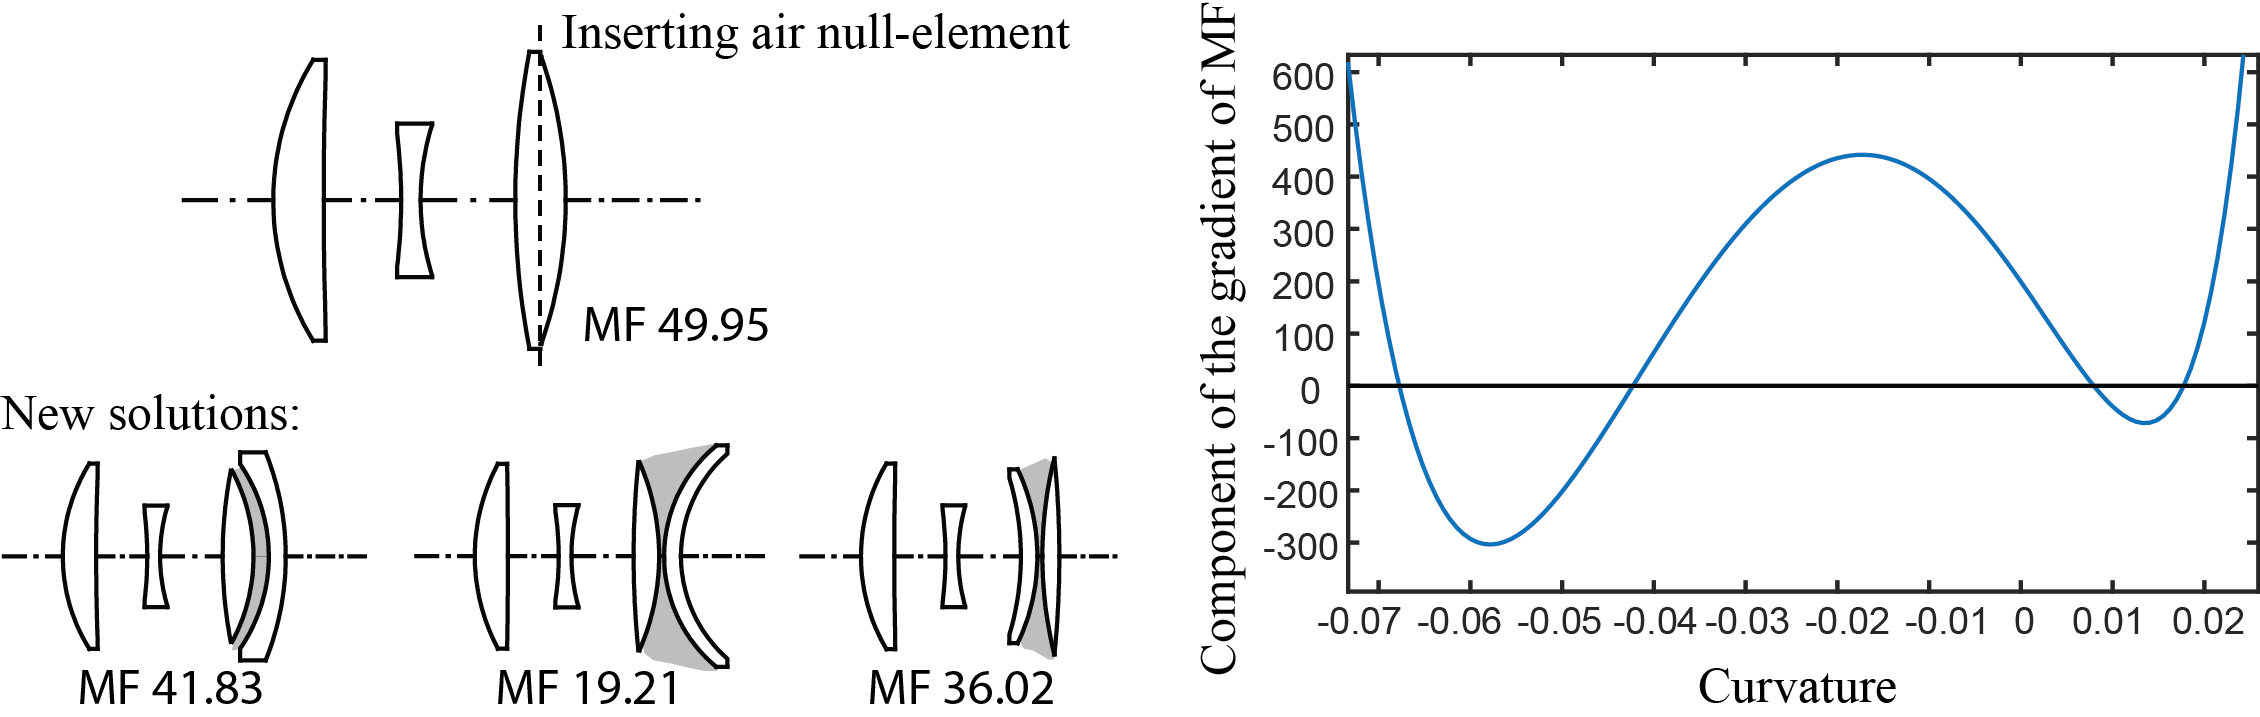
\includegraphics[scale=0.68]{chapter-2/figures/spc_add_air.png}
    \caption{Adding a lens element by adding an air null element using the SPC (splitting lenses). The dashed line indicates the SPC scan position. Four saddle points lead to three solutions with one lens more. The added air spaces are shaded. MF value of each system is listed, and the unit is $\mu m^2$. }
    \label{fig:SPC-air null element}
\end{figure}

\label{cp2-switching}
\subsection{Switching to alternative minima}

\subsubsection{The EXTRACT and ADD operation}
In practical lens design, it is usually important to obtain a better solution without changing the number of variables (lens elements). Adding extra elements in the system often means that the costs of the system become higher and that the system becomes less compact. 

When using the SPC, with some subsequent steps described below, it is possible to switch between local minima with the same number of variables. Illustrated in Figure \ref{fig:SPC-switch-example}, the first step is to choose which lens to modify. The middle one of the Cooke triplet was chosen in this example. The next step is to extract this element from the original system as follows. The thickness of the chosen element is gradually reduced to zero while in each step the system is optimized with respect to the remaining variables. Small steps should be applied for the change of the thickness to prevent the optimization moving to a different basin of attraction. When the basin of attraction of the optimization changes, a sudden change in the merit function value can be observed. After the thickness is reduced to zero, the curvatures of the two surfaces are usually different. Next the curvatures can be changed gradually until they become equal and the system is optimized with respect to the remaining variables after each step. 

\begin{figure}[h!]
    \centering
    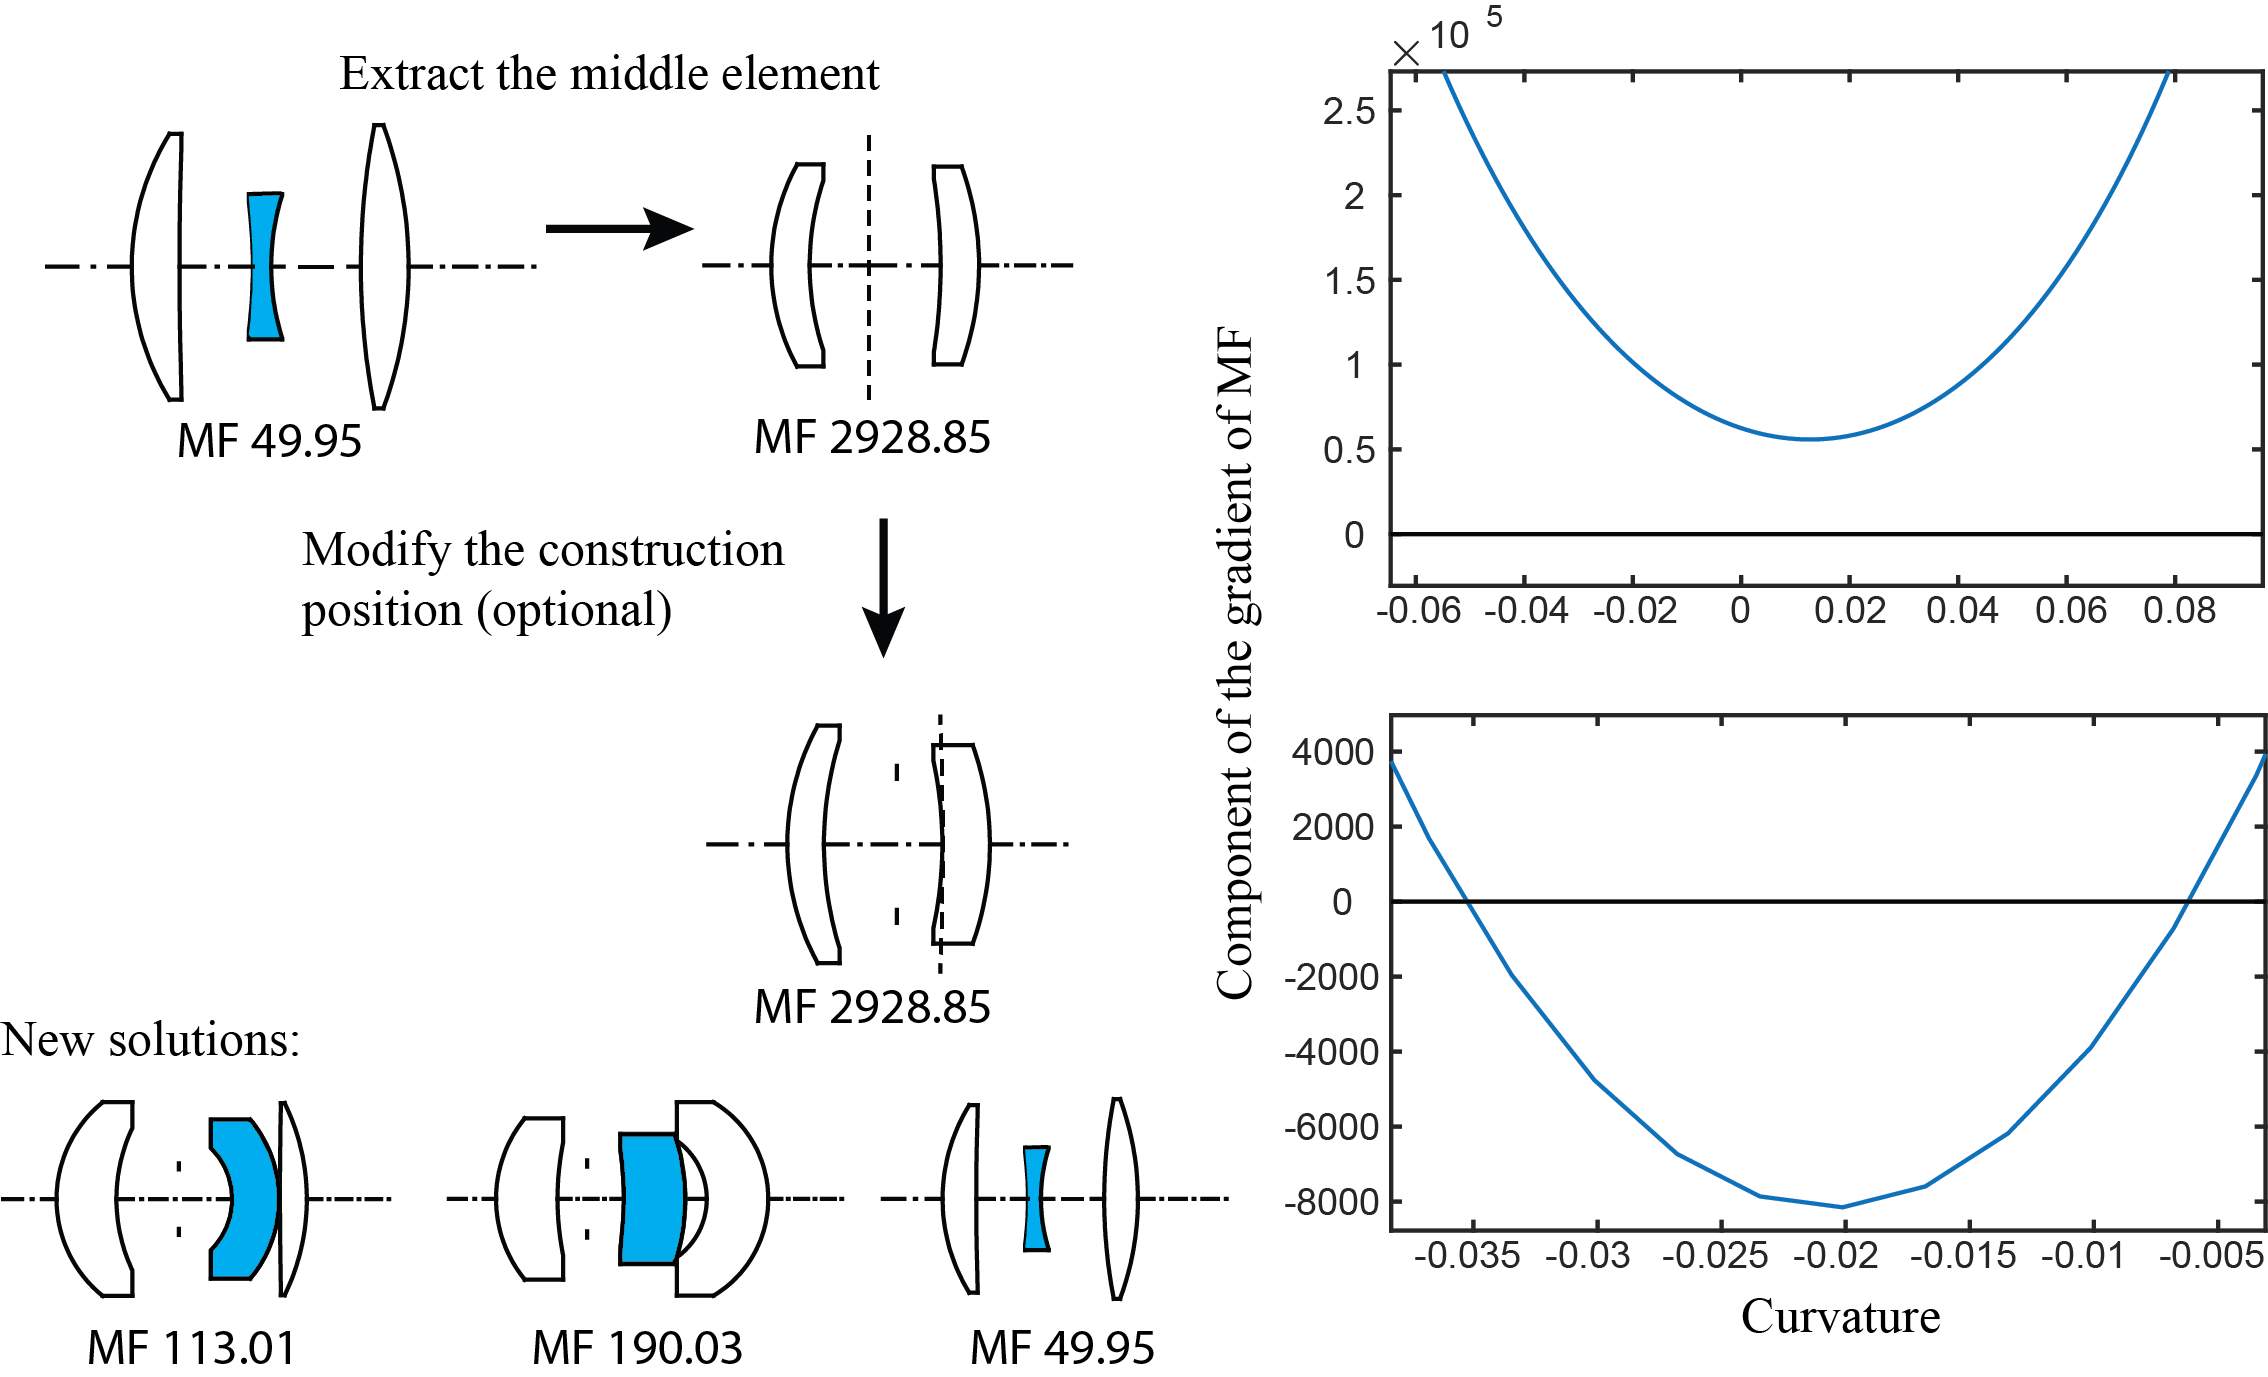
\includegraphics[scale=0.68]{chapter-2/figures/spc_switch.png}
    \caption{Switching to different solutions with the SPC. The middle lens element was chosen to be first extracted, and the SPC was performed at the same location. However, no saddle point was found in that location. The scanning location was then shifted right. Two saddle points and three solutions were obtained. MF value of each system is listed, and the unit is $\mu m^2$. }
    \label{fig:SPC-switch-example}
\end{figure}

Once the thickness of the chosen lens has been made zero and the two curvatures have been made equal by this procedure, the null element can be extracted from the system without changing the value of the merit function. In fact, we have now a system with one lens less which is a local minimum for the reduced number of variables. The system is ready to be inserted with null element in order to add back the extracted lens and obtain new local minima. The null element is usually inserted at the same location where the lens is extracted and the derivative of the merit function with respect to the curvature is scanned to search for saddle points. In Figure \ref{fig:SPC-switch-example}, the curve plot on the top shows the SPC scan when it is performed at the position of the extraction. It is seen that the scan shows no saddle point. The subsequent step is to change the position where the null elements is inserted in the space between the two lens elements. Where the arrow points down in Figure \ref{fig:SPC-switch-example}, the position of the insertion of a null element is chosen to coincide with the left surface of the right lens. The curve of the derivative has two zero-crossings, which indicates two saddle point systems. One of the saddle points can be explained by the special version of the SPC \cite{BociortSPCSexplained}, where the curves of the inserted element are identical to the surface which the null element is attached to. 

Three solutions were obtained from the two saddle points. After relaxing all variables and optimizing, the solution on the right in Figure \ref{fig:SPC-switch-example} becomes identical to that of the original Cooke triplet. The other two solutions are new solutions. None of the two shows better MF values compared to the Cooke triplet design. 


\subsubsection{The ADD and EXTRACT operation }
It was shown that with an extract-and-add strategy one can switch systematically from one local minimum to other minima, with the same number of variables. A intermediate step is necessary to first reduce the number of the variables in the original problem (by extracting a lens). 

It is also possible to switch to different solutions using the SPC by first increasing the number of variables: an add-and-extract strategy. However, it is not really recommended since it requires more decisions on where to add or extract in the intermediate steps. For an extract-and-add strategy, it is demonstrated in the previous section that the designer only needs to decide where to extract an element. In contrast, an add-and-extract strategy will work as follows: the designer first has to decide where to add an element to the original system. Then, after the SPC operation, usually more than one solution is produced. In the simplest case, the designer can decide to extract the same element for all of them. However, it is also possible to decide to extract different elements from the solutions obtained after SPC. In either way, the add-and-extract strategy will require more decision steps than the extract-and-add strategy.

%\subsection{Derivatives base on the technique provided}
\section{Conclusion}
In this chapter, the Saddle Point Construction (SPC) method is explained in detail. The method constructs saddle point system with Morse Index $1$ in a higher dimensional space (from dimension $N$ to dimension $N+2$). Optimizing from a saddle point of Morse Index $1$ can systematically lead to two local minima. The general version of the SPC involves a scan of the inserted curvatures to search for the saddle point. It is not guaranteed that the scan will generate saddle points. In the special version of the SPC a null element attached to an existing surface is added, where a saddle point system can be immediately obtained \cite{BociortSPCSexplained}. 

By performing a scan to find systems where the first order derivative of the merit function vanishes, the general version of SPC usually finds more than one saddle point, therefore, often several solutions are obtained. When such a scan of the derivative happens at a position same as an existing surface, the saddle point predicted by the special version of the SPC will also be included. 

Recommendations on how to use the SPC in practice are provided: an SPC scan can be done either by scanning a glass null element (adding a lens element) or scanning an air null element (splitting a lens element).  Depending on the scan positions, the two approaches can produce similar solutions ( e.g. Figure \ref{fig:SPC-glass null element} and Figure \ref{fig:SPC-air null element}).

Switching to different local minima using the SPC without increasing the number of elements (ie. variables), can be very useful. This is realized by first extracting a lens element, and then performing an SPC scan at the extracted position. Figure \ref{fig:SPC-switch-example} demonstrates the steps where extra solutions are obtained. 

In the following two chapters, the SPC is used in the way described in this chapter. A detailed study of the saddle point - minima networks using SPC is presented in Chapter 3. Several practical examples are given in Chapter 4 demonstrating how these approaches can be used in lens design. 


\references{dissertation}


\setlength{\parskip}{.2em}
\graphicspath{ {./chapter-3/figures/} }
\captionsetup[figure]{labelfont=bf}
\captionsetup{margin=1.5em}
\captionsetup[table]{labelfont=bf}


\chapter{Lens Design Landscape Exploration with Simple Systems}
\label{chapter_SPC_simple_system_landscape}

%% The following annotation is customary for chapter which have already been
%% published as a paper.
\blfootnote{Parts of this chapter have been published in Applied Optics \textbf{55}, 10449 (2016) \cite{HouSimple16}.}

%% It is only necessary to list the authors if multiple people contributed
%% significantly to the chapter.
%\authors{Albert {\titleshape Einstein}}

% %% The '0pt' option ensures that no extra vertical space follows this epigraph,
% %% since there is another epigraph after it.
% \epigraph[0pt]{
%   A journey of a thousand miles begins with a single step
% }{Laozi}

% \epigraph{
%     Sample quotes
% }{author}

% \begin{abstract}
% Previous researches have shown that different solutions of the optical system can be found using saddle point based method for some simplified cases\cite{PascalTriplet2009}. It is important, however, to study whether the saddle point based method still perform well in practical lens design problems. To study this, we chose to start with a relative simple example.
% \end{abstract}

% %% Start the actual chapter on a new page.
% \newpage

\noindent 
In a lens design landscape, from a saddle point system with Morse index $1$, optimization will lead to two solutions of local minima.  When performing a SPC \footnote{The definition of "performing an SPC scan" is given in Chapter \ref{spc-general}.}, it can find several saddle point configurations, which subsequently lead to multiple local minima. 

Therefore, it is an intriguing question whether or not the local minima in the design landscape are all connected by the saddle points of Morse index $1$. If this is the case, then by constructing sufficiently many saddle points, in principle all local minima of the design landscape can be obtained. 

This chapter is mainly based on a research paper\cite{HouSimple16} published in 2016. It is shown that in the design landscape of a wide-angle pinhole lens and in closely related optimization landscapes, all good local minima found by other methods can be obtained easily with a succession of one-dimensional searches (SPC scans) starting from simpler systems. By replacing high-dimensional searches with a succession of one-dimensional searches, the design efficiency can be increased significantly. By combining this method with conventional design methods, the wide-angle pinhole lens can be designed starting from a single lens.

% Reason for choosing the wide-angle pinhole lens. 1) Application wise, it is application wise popular. 2) It is sufficiently different from the previous studied ideal examples.
In a 2004 research paper \cite{BociortThinLens2004}, Bociort et al. show that when some general mathematical requirements are satisfied, %{a thin lens model is used, and only the spherical aberration is considered, }
the minima and saddle points in the lens design landscape form a network. The saddle points in this network can be theoretically predicted, hence from the saddle points, minima are obtained. Research conducted by Van Grol et al.\cite{PascalTriplet2009} claims that there is a fundamental network for a lens design problem with a certain number of lenses. In their paper, examples of the fundamental network of doublet and triplet systems are given. The authors predict that in practical design cases, the types of system shapes \footnote{In a lens system, each lens element has its lens form: biconcave, biconvex, meniscus, etc. The type of the system shape of a lens system is determined by the combination of the individual lens forms. For example, a biconcave-biconvex doublet is one type of system shape, and a biconcave-meniscus is a different type of system shape. } of the solutions will not exceed the types of system shapes from the fundamental network. In a later paper from 2010\cite{BociortTripletExplained2010}\cite{BociortToyModel2010}, Bociort shows that a toy model based on third-order spherical aberration can be used to mathematically explain the fundamental network of the triplet. 

For the assumption that the dominant aberration is spherical aberration, and that the lenses are not too thick, it is possible to predict the existing solutions within the network. However, in practical cases, aberrations other than spherical aberration will also determine the topology of the merit function landscape. In this case, it is mathematically too complex to build an analytical model to predict the behaviour of the merit function landscape.

Despite the complexity to use an analytic model to predict the merit function landscape, earlier research shows \cite{BociortSPCSexplained}\cite{MVTurnhoutSPC15} that in the lens design space, a special structure is present that makes the lens design problem different from a general global optimization problem: certain saddle points existing in the landscape are reducible to minima of simpler systems with one lens element less. Using this structure, the SPC \cite{MVTurnhoutSPC15} method is developed to obtain new design solutions. In the conventional approach, trial and error is needed to look for different solutions (if there is more than one) by adding one extra lens element to the existing system. With the SPC, there is a systematic procedure to search for available solutions by adding new elements to the system. When starting from a minimum with $N$ variables, with SPC it is possible to systematically find minima in an $(N+2)$-dimensional variable space by using one-dimensional searches, rather than $(N+2)$-dimensional searches. Important questions are, however, how many minima existing in the landscape can be obtained in $(N+2)$-dimensional search spaces, by replacing high-dimensional searches with one-dimensional searches? What percentage of them can be found? Is it possible to at least obtain the good solutions? In this chapter, the performance of SPC is evaluated for more general problems, especially those of practical interests. 


%%%%%%%%%%%%%%%%%%%%%%%%%%%%%%%%% Section 1 %%%%%%%%%%%%%%%%%%%%%%%%%%%%%%%%%%%%%%%
\section{Wide-angle Pinhole Lens}

A wide angle pinhole lens, designed by Irina Livshits from ITMO, has been chosen to study the design landscape using SPC. For surveillance applications, this kind of lens, has in recent years, become very popular. Instead of a lensless optical element, the pinhole lens here refers to a lens having an aperture stop with a small diameter placed in front of the system. All lenses are in contact, one lens is cemented, and three different glass materials are used [see Figure \ref{fig:widepinLens}(a)]. The design specifications are given in Table \ref{table: sysspec} and the surface specifications are provided in Appendix \ref{apdx: wide-angle-specs_4_elements}. In Figure \ref{fig:widepinLens}(b) a 2D image simulation made with CODE V shows that, despite its simplicity, the system has an imaging quality that is adequate for its intended purpose. The system can also be adapted for spectral imaging applications \cite{Strauch2015}. For optimization we use the default CODE V merit function that is based on transverse ray aberrations. The value of the merit function (called in CODE V error function) for this system is 5.68 \textmu m$^2$. It is a composite value, scaled so that it is the mean square of the weighted image radius. The value has considered a setting with three wavelengths as shown in Table \ref{table: sysspec}. In the following text in this chapter, values of the merit function are presented without adding the unit. 

\begin{figure}[h!]
    \centering
    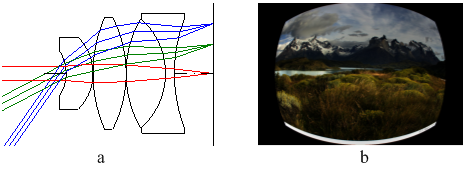
\includegraphics[scale=0.95]{chapter-3/figures/WidePinLens.png}
    \caption{Wide-angle pinhole lens. (a) Lens drawing. (b) 2D image simulation of its imaging quality.}
    \label{fig:widepinLens}
\end{figure}

\setlength{\arrayrulewidth}{.5mm}
\setlength{\tabcolsep}{18pt}
\renewcommand{\arraystretch}{1.2}
\begin{table}[h!]
    \centering
    \captionsetup{justification=centering}
    \caption{System specification}
    \label{table: sysspec}
    \vspace{-1em}
    \begin{tabular}{ p{20em} c }
    \hline 
    Entrance Pupil Diameter (EPD, mm) & 0.8\\
    (Full) Field Of View (FOV, °) & 110\\
    Effective Focal Length (EFL, mm) & 3.5\\
    Wavelength (nm) & 644, 546, 480\\
    \hline
    \end{tabular}
\end{table}



%%%%%%%% SECONTION Switching %%%%%%%%%%%%%%%%%%%%%%%
\section{Switching Between Local Minima}

To find other possible solutions for the same specifications, two different global optimization methods are used, Global Synthesis from CODE V \cite{KuperGO1992}\cite{RogersGO2006} and a saddle point detection method (the program NETMIN\footnote{NETMIN is a tool developed in TU Delft to search for new local minima based on saddle point detection method. Detailed description can be found in Chapter \ref{method: spd}.}). In this example, for simplicity only the surface curvatures are used as variables. Minor edge thickness violations, which can be easily corrected in a later stage, are acceptable in this analysis. 

It is of interest to find the so-called stable solutions, i.e., the solutions that do not easily appear or disappear when specifications are slightly changed. Three stable solutions are found, denoted in Figure \ref{fig:wideangleSwitch} by M1, M2, and M3. They exist for a wider range of specifications, e.g., not only for the field of view (FOV) of 110° as shown in Table \ref{table: sysspec}, but also for a FOV of 90°, and not only for an effective focal length (EFL) of 3.5 mm (for which the corresponding merit function values are 5.68, 11.51, and 11.09, respectively) but also for an EFL of 3.0 mm (with merit function values of 6.80, 23.20, and 16.70). These solutions have no large edge thickness violation and relatively low merit function values. From the lens drawings of these solutions, we observe that the second element differs significantly between them. A few solutions with low stability and large merit function values can also be found. They exist for instance either at EFL 3.5 mm or at EFL 3.0 mm, but not at both. Since these solutions with low stability appear or disappear easily when the EFL is changed, it is reasonable to assume that their basins of attraction (i.e., the set of starting points in the variable space that after optimization converge to the given solution) are small and therefore the risk that the optimization gets trapped in these basins is rather low. The solutions with low stability will therefore be ignored in what follows. While no global optimization method can guarantee that all minima are found, the landscapes examined in this research are simple enough so that there is a high probability that all minima having a basin of attraction large enough to be relevant, are found with the methods being used. 

\begin{figure}[h!]
    \centering
    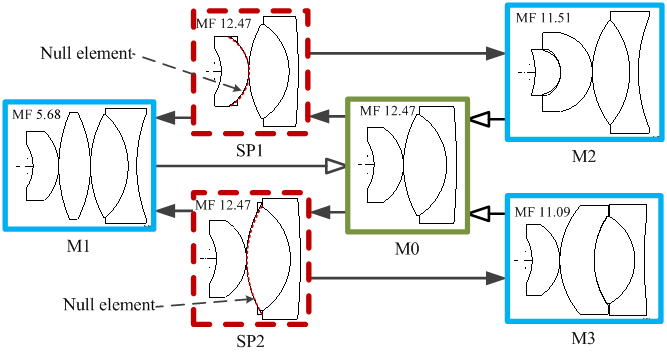
\includegraphics[scale=0.6]{chapter-3/figures/WideAngleSwitch.png}
    \caption{Switching between minima (blue boxes) using SPC. Extraction of the second element from M1, M2, or M3 results in the system M0 (hollow arrows). Starting from M0, two routes, each having an SP, lead to three different minima (solid arrows). The two saddle points shown in dashed red boxes can be found both by the general and by the special version of SPC. In SP1, the null-element has the same curvature as the second surface of M0; in SP2, it has the same curvature as the third surface of M0 (because of two zero thicknesses, we see there three overlapping surfaces, marked by red dashed line).}
    \label{fig:wideangleSwitch}
\end{figure}

Optimization can be trapped in the sub-optimal minima M2 and M3, which are significantly worse than M1. However, the global minimum M1 can be rapidly obtained with SPC from both of them. In M2 or M3, the second element is extracted first and then the SPC method is applied (suitable candidate lenses for extraction are in general weaker-power lenses that seem to have little function). After extraction and optimization, both solutions become the M0 system shown in the green box in Figure \ref{fig:wideangleSwitch} Then two saddle point systems, SP1 and SP2 in Figure \ref{fig:wideangleSwitch} (in the red dashed boxes), were constructed from M0 by adding a null element in between the first and the second lens (i.e., at the position of extraction). From each saddle point system, two local minima can be found after optimization. In this case, both saddle point systems lead on one side to the same minimum, the global minimum M1. On the other sides, the two saddle points lead to M2 and M3. In fact, from any of these three minima, the other two can be found by a switching operation. In this example, different ways of using the SPC method described in Chapter 2 are demonstrated: firstly, the SPC method can systematically find new solutions with more lenses (M1, M2, and M3) from a simpler system (M0); secondly, extracting and then adding lenses with the SPC can lead to different minima in a systematic way. This possibility of switching between different local minima is a typical property of the SPC.
%%%%%%%%%%%%%%%%%%%%%%%%%%%%%%%%%%%%%%%%%%%%% Section %%%%%%%%%%%%%%%%%%%%%%%%%%%%%%%%%%%%%%%%%%%%%%%%
\section{Designing a Pinhole System Starting from a Single Lens} \label{chrom90d}

In the previous section, by using SPC, we show how different designs can be found systematically by increasing the number of lenses. By using this approach in combination with traditional methods, it is possible to design an optical system starting with just one lens. This part shows how a pinhole lens similar to the one in Figure \ref{fig:widepinLens}(a) can be obtained from a single lens. The specifications are listed in Table \ref{table: sysspec}. The same merit function as before, is used.

A global optimization is performed starting from a plane parallel plate. Only one singlet solution is obtained, with a merit function value of 576.30, as shown on the left in Figure \ref{fig:WideAngleDesign}(a). This singlet serves as a basic element, providing optical power to the system \cite{LivshitsQA2013}. On this singlet, SPC is performed by adding a zero-thickness glass element at the back surface. Two doublet minima are found, with merit function values 164.81 and 1783.94 (the latter one disappears if we replace EFL 3.5 mm by, e.g., EFL 3.0 mm). The better one (the first one) is chosen for the next design step. 

\begin{figure}[h!]
    \centering
    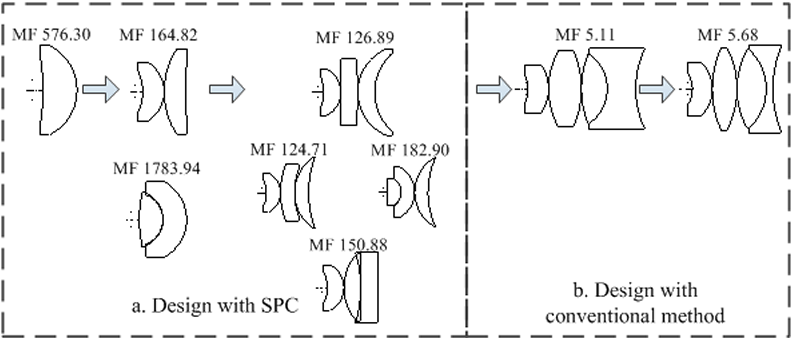
\includegraphics[width=1.0\textwidth]{chapter-3/figures/WideAngleDesign.png}
    \caption{Designing a wide-angle pinhole lens from one lens by combining SPC with conventional methods.}
    \label{fig:WideAngleDesign}
\end{figure}

With the same strategy, SPC is performed on four different surfaces of the doublet with a merit function value of 164.82 and four triplet minima are found (with merit function values 124.71, 126.89, 150.88, and 182.90, respectively). Only one type of glass is used for the steps mentioned above. In the next step, we continue with the best two minima using conventional design techniques: glasses are changed and the third lens is replaced with a cemented doublet to correct chromatic aberrations. The glasses are selected to be the same as the original system designed by Irina Livshits. When the glass are modified, the best minimum (a merit function value of 124.71) of the triplets encounters ray failure. However, the system with a merit function value of 126.89 still remains stable after changing the glass. Optimization with all curvatures and thicknesses as variables leads to a system with a merit function value of 5.11 [Figure \ref{fig:WideAngleDesign}(b)]. By readjusting the thickness of the lenses for a more compact size, a system with the merit function value of 5.68 was obtained [see Figure \ref{fig:WideAngleDesign}(b)], which is identical to the original design in Figure \ref{fig:widepinLens}(a).

SPC is useful for dealing with minima created by monochromatic aberrations. It cannot deal directly with minima created by chromatic aberrations. However, since typically chromatic aberrations are less non-linear than monochromatic ones (e.g., unlike the Seidel aberrations, for axial chromatic aberration the thin-lens expressions are linear), the chromatic aberrations tend to create fewer new minima than the monochromatic
ones. As shown in this example, in the design process SPC can be easily combined with traditional approaches to handle chromatic correction.

In addition, four triplet minima are found with the SPC method in the search using only one glass, as shown in Figure \ref{fig:WideAngleDesign}(a). Both Global Synthesis \footnote{It is a proprietary global optimization algorithm of CODE V. The algorithm starts from the given system and explore solutions space for new configurations in a systematic manner.} and saddle point detection
(NETMIN) finds only three minima (missing the one with the merit function value of 182.90). Therefore in this example, the SPC method has the advantage of being able to find more minima than the two methods used for comparison. 

%%%%%%%%%%%%%%%%%%%%%%%%%%%%%%%%%%%%%%%%%%%%% Section %%%%%%%%%%%%%%%%%%%%%%%%%%%%%%%%%%%%%%%%%%%%%%%%
\section{Decomposing a High-dimensional Search for New Minima in a Succesion of One-dimensional Searches}  \label{chrom60d}

It is mentioned in the previous section that the SPC found more system candidates compared to the Global Synthesis of CODE V and the saddle point detection algorithm. However in the examples, the number of minima found in the landscape is small. In this section it is investigated whether the performance of SPC is still good when more minima are present in the landscape.

In order to generate more minima, the FOV of the triplet system is reduced to 60° while the other specifications remained as that given in Table \ref{table: sysspec}. The reason why a reduced
field leads to more minima will be discussed in the next section.
As in Figure \ref{fig:WideAngleDesign}(a) only one type of glass is used, the variables are only the curvatures. The same default CODE V merit function is used, and, for the purpose of this study, the control of edge thickness is disabled. All lenses are in contact (i.e., all air spaces between lenses have zero thickness). The thicknesses of all lenses in a minimum system are set equal in order to avoid the multiple appearance of essentially the same minima (with similar curvatures, but different lens thicknesses) that would unnecessarily complicate the study \cite{HouProc2015}.

For a better understanding of the results, in addition to the comparison of minima, it is also useful to compare the saddle points obtained using SPC with those obtained using the saddle point detection algorithm (realized by the program NETMIN). For SPC there are the options of inserting in the existing minimum either a glass null-element (i.e., inserting a lens) or an air null-element (i.e., splitting a lens). If the zero-thickness glass element was used, the saddle points resulting from the SPC scan would still have a zero-thickness lens, whereas the saddle points detected with NETMIN would have finite thicknesses for all lenses. This is because that the NETMIN starts from existing minima with non-zero thickness element and searches for the saddle points. The saddle points obtained from the two methods can not be directly compared due to the thickness differences of the lens element. In our study, all lens elements are set to be in contact. In this case, the saddle points detected with NETMIN will have zero air spaces. It is therefore better for comparison to study the performance of the SPC when air null elements are used. Splitting lenses with SPC leads to saddle points with a zero distance between lenses, which are directly comparable with the saddle points from NETMIN. For performing SPC with a zero-thickness air element, the thickness of the lens, which will be split, is first doubled. Then the system is re-optimized to a minimum, and a zero-thickness air element is inserted in the middle of the lens. As mentioned in section \ref{section: SPC recommendation}, the example of Cooke triplet shows that the minima are different between applying zero-thickness glass and zero-thickness air space constructions. Therefore, both approaches are recommended to be used. However, in this example, it turns out that SPC with zero-thickness glass does not give more local minima than using zero-thickness airspace. For simplicity and better comparison, the SPC result using zero-thickness air space is shown. 
\begin{figure}[h!]
    \centering
    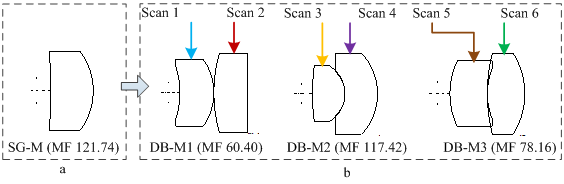
\includegraphics[width=0.8\textwidth]{chapter-3/figures/Single2Double.png}
    \caption{SPC by inserting a zero-thickness air element. (a) Singlet solution (SG-M). (b) The three doublet minima (DB-M) that result from the singlet are the starting minima for the scans shown in Figure \ref{fig:tripletnetwork}.}
    \label{fig:single2double}
\end{figure}

As previously, we start with a single optimized lens [SG-M shown in Figure \ref{fig:single2double}(a)] and three doublets are obtained with the SPC [shown in Figure \ref{fig:single2double}(b)]. The three doublets DB-M1, DB-M2, and DB-M3 have a total of six lenses.  Each of the six lenses is used to generate an SPC scan which leads to triplet minima. The colored arrows in Figure \ref{fig:single2double}(b) indicate the lenses that are split (after the thickness doubling that is not shown here) in the corresponding scan.

Figure \ref{fig:tripletnetwork} shows the minima and saddle point systems found in the triplet design space with NETMIN and Global Synthesis (Global Synthesis has found nine out of 10 minima, missing the minimum M6). Five curvatures are used as variables, and the curvature of the last surface is controlled by a \textit{Solve} in CODE V to keep the effective focal length constant.

A significant result of this search is that all 10 triplet minima shown in Figure \ref{fig:tripletnetwork} are also obtained with SPC starting from the three doublets in Figure \ref{fig:single2double}. Eleven saddle point systems are obtained from the six one-dimensional SPC scans. Different scans find different numbers of saddle points. For instance, in Scan 2 there are four saddle points (SP1, SP2, SP7, and SP8 in Figure \ref{fig:tripletnetwork}), whereas in other scans, only one or two saddle points are found. The 10 minima are resulted from the 11 saddle point systems by optimising on both sides of the saddle. Saddle point systems and minima obtained from the same scan are connected in Figure \ref{fig:tripletnetwork} with the same colored lines. In the figure, when we gradually increase the FOV, M1 corresponds to the system leading to the final design in the 110° case [merit function value 126.89 in Figure \ref{fig:WideAngleDesign}(a)]. However, in this case, its merit function value of 61.14 is not the smallest one in Figure \ref{fig:tripletnetwork}.

NETMIN finds the extra saddle point system SP12, which cannot be found by SPC. This saddle point system connects with a dashed link the minima M3 and M9 in Figure \ref{fig:tripletnetwork}. However, there is sufficient redundancy in the SPC approach, and both M3 and M9 also result from other saddle point systems which are found by SPC. Therefore the lack of ability of SPC to find SP12 is not critical.

Since there are five variables, with general global optimization tools this search has to be performed in a five-dimensional space. In this example, however, all minima found with other methods are also found with SPC, where the five-dimensional search is replaced by six one-dimensional searches. Replacing a high-dimensional search for new minima by a succession of one-dimensional searches reduces the complexity of the search significantly.

The example discussed above shows the utility of the feature of the optical merit function landscape that enables the decomposition of the search for many of the minima in simpler steps. The feature means that minima and saddle points are all connected, and the saddle points can be constructed by SPC. This example has the advantage that in this case, the feature mentioned above can be observed in a pure form, without interference from other features (e.g. the minima are not connected by saddle points that can be constructed) of the landscape. However, in general, other features which deserve further study to gain a better understanding, may also play a role. Therefore, it cannot be expected that we can always find all minima using SPC. Nevertheless, even when other features are present, examples studied so far show that SPC can lead to satisfactory results.

For instance, when the search described in Figure \ref{fig:tripletnetwork} is repeated with modified wavelength specifications, SPC finds 11 minima and Global Synthesis finds 10 (see Figure \ref{fig:TripletMonoNetwork}). Among these minima, eight, including the best five, are found by both methods. For the four minima that are missed by SPC, two of them are unphysical (minima 12 and 14, they have either negative or zero back focal length that cannot be corrected, but should be prevented with an additional constraint). These unphysical solutions also have a merit function more than 4 times and more than 50 times that of the best solution. The other two minima missed by SPC (minima 13 and 15) have merit function values 40 times and 8 times that of the best solution. NETMIN finds all four solutions missed by SPC, and Global Synthesis finds two of them.

% \begin{figure}[h!]
%   \begin{adjustbox}{addcode={%
%     \begin{minipage}{\width}}{%
%     \captionsetup{margin=0em}
%     \caption{Network of minima (solid boxes) and SP systems (dashed boxes) in the 60° landscape, where the other specifications are the same as in Table \ref{table: sysspec}. Eleven SP systems result from six SPC scans (each color represents one scan). Optimization starting at these SP systems leads to all 10 minima that were obtained with NETMIN and Global Synthesis. If in any of these 11 SPs we remove the null-element of the corresponding scan (this does not affect the ray paths or the MF), we obtain the starting doublet of the scan. The null elements are marked by crosses with the corresponding color. This figure shows why the lens design landscape is different from general global optimization landscapes: because of the close relationship that exists between local minima of a design problem (here the 10 triplet minima) and local minima with one lens less (here the starting doublets).}\label{fig:tripletnetwork}
%     \end{minipage}},rotate=90,center}
%     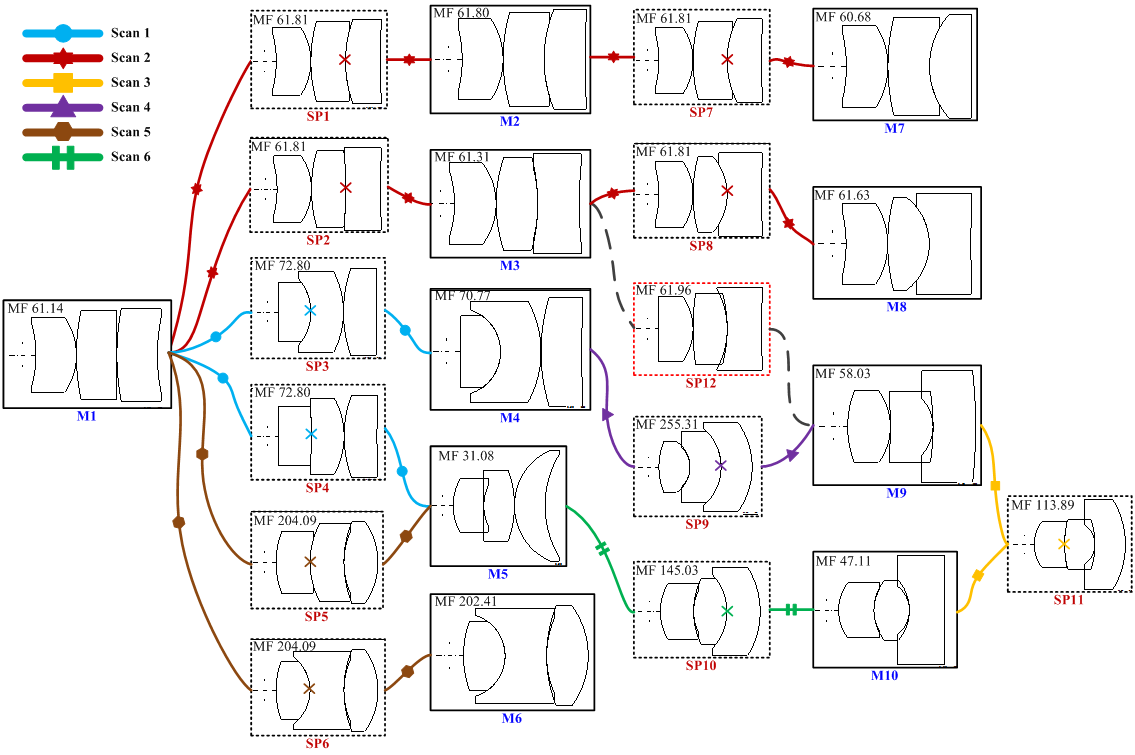
\includegraphics[scale=0.5]{chapter-3/figures/TripletNetwork.png}
%   \end{adjustbox}
% \end{figure}

\begin{figure}[h!]
    \centering
    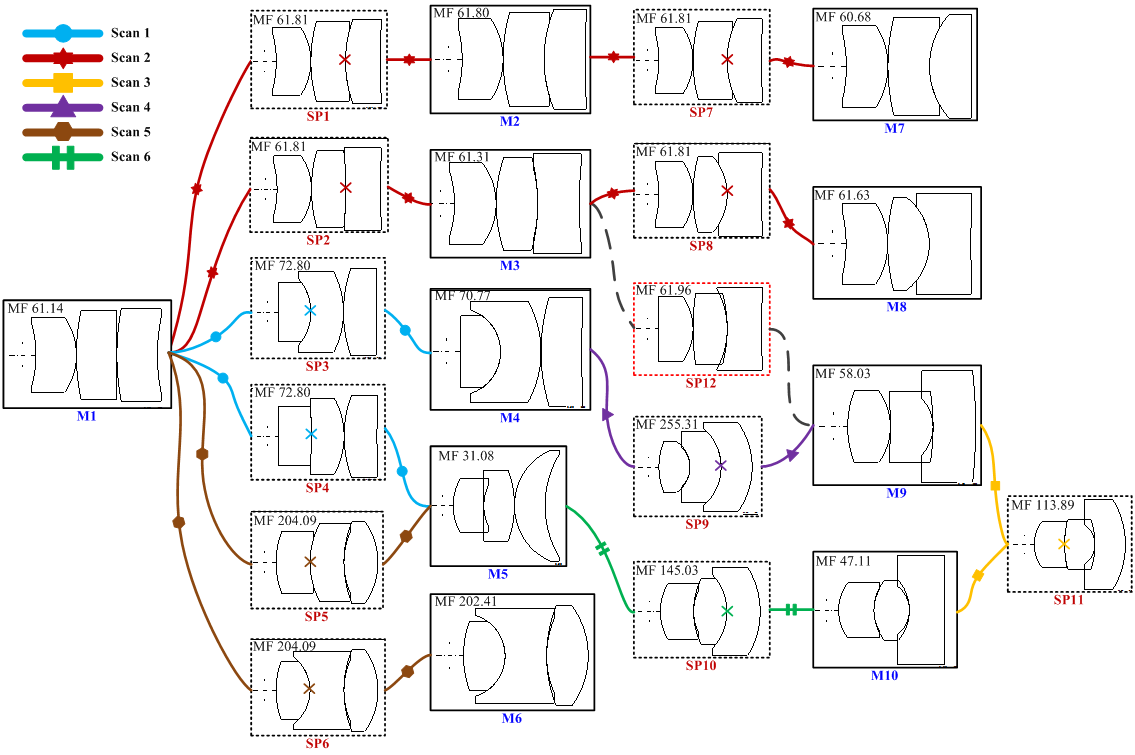
\includegraphics[scale=0.41]{chapter-3/figures/TripletNetwork.png}
    \caption{Network of minima (solid boxes, named as M\#) and saddle point systems (dashed boxes, named as SP\#) in the 60° landscape, where the other specifications are the same as in Table \ref{table: sysspec}. Eleven saddle point systems result from six SPC scans (each color represents one scan). Optimization starting at these saddle point systems leads to all 10 minima that are obtained with NETMIN and Global Synthesis. If in any of these 11 saddle points we remove the null-element of the corresponding scan (this does not affect the ray paths or the merit function), we obtain the starting doublet of the scan. The null elements are marked by crosses with the corresponding color. This figure shows why the lens design landscape is different from general global optimization landscapes: because of the close relationship that exists between local minima of a design problem (here the 10 triplet minima) and local minima with one lens less (here the starting doublets).}\label{fig:tripletnetwork}
\end{figure}

Despite the fact that SPC cannot find four (poor-quality) minima directly, it turns out that by using the switching strategy described earlier, it is easy to escape from any of them if optimization is trapped. Eliminating a lens from any of these poor-quality minima leads to one of the three doublets. From these doublets, better minima can be obtained with SPC.
\begin{figure}[h!]
    \centering
    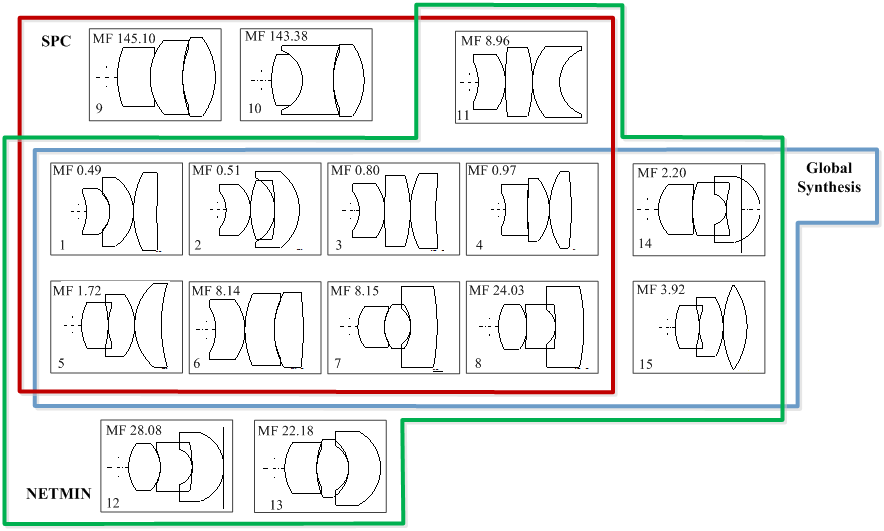
\includegraphics[width=1.0\textwidth]{chapter-3/figures/TripletMoNoNetwork.png}
    \caption{Minima found with SPC (red box), Global Synthesis (blue box), and NETMIN (green box) in a monochromatic run. Minima 12 with Merit Function (MF) value 28.08 and Minima 14 with MF value 2.20, whose image planes are inside or coincide with the last lens, are unphysical. The five minima with the lowest MF value (numbered from 1 to 5) are found by all three methods. Edge thickness violations is disabled in this search.}
    \label{fig:TripletMonoNetwork}
\end{figure}

However, in order to understanding the potential and the limitations of SPC, it is useful to examine why SPC is not able to reach these four minima. SPC is based on the assumption that small changes in lens thicknesses do not affect good designs significantly, i.e., that good minima continue to exist as minima when a reasonably small non-zero thickness is replaced by zero. This assumption is similar to the one at the basis of the well-known thin-lens aberration theory. In earlier days of lens design, primary aberration formulas using zero thickness were used to qualitatively predict the existence of good designs.

It turns out that the minima that are not found by SPC only exist for certain non-zero thickness values and do not have a zero-thickness equivalent. However, the existence of these minima does not contradict our assumption that using SPC can obtain satisfactory solutions, because these are not among the best solutions. In the numerical experiment, final solutions have the same thickness for each lens element (1.5 mm). Since in the SPC procedure the practical design is always obtained after increasing the zero-thickness of a null element, it is not possible to reach minima that disappear when the lens corresponding to the null element has zero thickness. In NETMIN and Global Synthesis searches, the lens thicknesses are kept constant. This typical behavior is illustrated in Figure \ref{fig:thicknesschange}(a) and (b). In the system in Figures \ref{fig:thicknesschange}(a) found by SPC, the thickness of the first lens is 1.5 mm. By starting with a zero-thickness null-element as the first lens as in Figure \ref{fig:thicknesschange}(b), increasing the thickness leads to the system in Figure \ref{fig:thicknesschange}(a). By decreasing the thickness of the first lens of the system in Figure \ref{fig:thicknesschange}(a), the system in Figure \ref{fig:thicknesschange}(b) is obtained. In contrast, in the system in Figure \ref{fig:thicknesschange}(c) found by NETMIN but not by SPC, when the thickness of the first lens is decreased ray failure occurs and a system with zero-thickness element cannot be obtained. However, systems like the one in Figure \ref{fig:thicknesschange}(c) have low stability. A small perturbation on the system in Figure \ref{fig:thicknesschange}(c) will lead to the system in Figure \ref{fig:thicknesschange}(a).

\begin{figure}[h!]
    \centering
    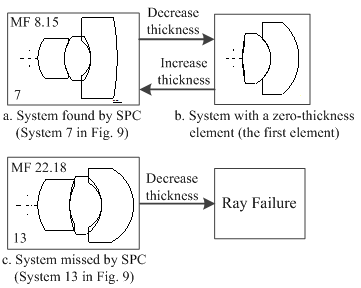
\includegraphics[scale=0.7]{chapter-3/figures/thicknesschange.png}
    \caption{Increasing the thickness of the first element of system (b) results in system (a), and vice versa. System (b), which is obtained by the SPC, is a minimum with a zero-thickness element. System (c), which is missed by the SPC, does not have a corresponding zero-thickness pair. A small perturbation on system (c) will lead to system (a).}
    \label{fig:thicknesschange}
\end{figure}


%%%%%%%%%%%%%%%%%%%%%%%%%%% Section %%%%%%%%%%%%%%%%%%%%%%%%%%%%%%%%%%%%%%%%%%%
\section{Effect of Changing the Field of View on the Landscape}
In Section \ref{chrom90d} and \ref{chrom60d} it is found that when the field of view is reduced, more minima can be found in the design space. This happens for two reasons. First, when design specifications (e.g., FOV or EPD) are modified, the distances in the design space between minima and saddle points change
and therefore the merit function landscape also changes. As can be observed in numerical experiments, when a minimum and a saddle point with Morse Index $1$ collide, they both disappear. Alternatively, such a pair can appear when specifications are changed. Similarly, two minima with a saddle point between them can be replaced by one minimum, and two saddle points with a minimum between them can be replaced by an SP. This can be explained mathematically by the conservation of the topological degree of the merit function landscape \cite{vanTurnhoutThesis2009} \cite{KoornwinderTopologicaldegree}. The topological degree of a critcal point is the sign of the determinant of the Hessian matrix in that point. The degree of a critical point is thus $(-1)^{Morse Index}$. A minimum has a topological degree of $+1$ and a saddle point with Morse Index $1$ has a topological degree of $-1$. The sum of the topological degrees remain constant under perturbation such as changing the FOV. Second, when the FOV is increased ray failure appears more easily, and the region of ray failure expands in the design space. Because certain minima and saddle points which exist for lower FOV cross the border of the ray failure region and disappear, fewer of them are found at large FOV.

 When varying the FOV of the systems shown in Figure \ref{fig:tripletnetwork}, the number of solutions changes with the FOV as shown in Figure \ref{fig:FOVvarying}. Three different FOVs are chosen: 110°, 90° and 60°. Six solutions were obtained for 110°, five for 90° and ten for 60°. From Figure \ref{fig:FOVvarying}, it is seen that some system shapes exist in all the three FOV configurations. However, other system shapes only exist in the specific FOV range.
For FOV 60°, five new systems, which did not exist for a larger field (second row for the 60° systems in Figure \ref{fig:FOVvarying}). The dashed boxes in Figure \ref{fig:FOVvarying} mark the missing systems which exist in other FOV specifications. As mentioned in the previous paragraph, the appearance and disappearance of the systems can be explained by the change of the merit function landscape. 

\begin{figure}[h!]
    \centering
    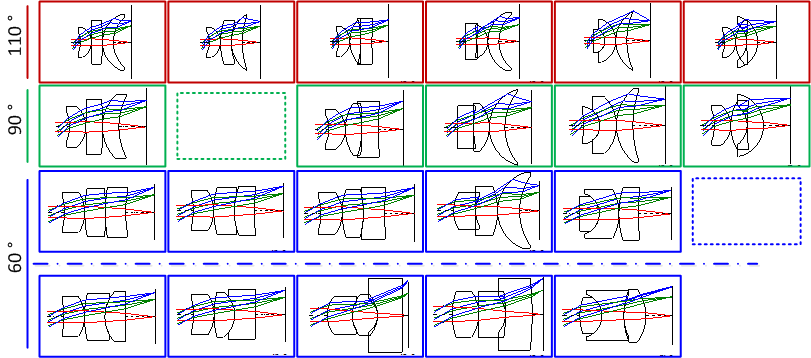
\includegraphics[width=1.0\textwidth]{chapter-3/figures/FOVvarying.png}
    \caption{For different field of view, the number of solutions is different. Systems with 110° FOV have six solutions marked by the red colour; Systems with 90° have five solutions marked by the green colour; Systems with 60° marked by the blue colour. The dashed boxes mark the missing systems.}
    \label{fig:FOVvarying}
\end{figure}

These phenomena can also be observed by examining the SPC scan curves. Figure \ref{fig:phasechange_field} refers to Scan 2 of Figure \ref{fig:tripletnetwork} where five minima are linked by four saddle points, and the FOV is 60°. In Figure \ref{fig:phasechange_field}, the scans are performed in different FOV settings: the FOV of the system increases from 50° [Figure \ref{fig:phasechange_field}(a)] to 90° [Figure \ref{fig:phasechange_field}(d)]. With the increase of the FOV, the ray failure region (shown as shaded area) is seen to expand. Two saddle points are found at 70° [Figure \ref{fig:phasechange_field}(c)], however, at 90° [Figure \ref{fig:phasechange_field}(d)] the most left saddle point disappears into the ray failure region.
\begin{figure}[h!]
    \centering
    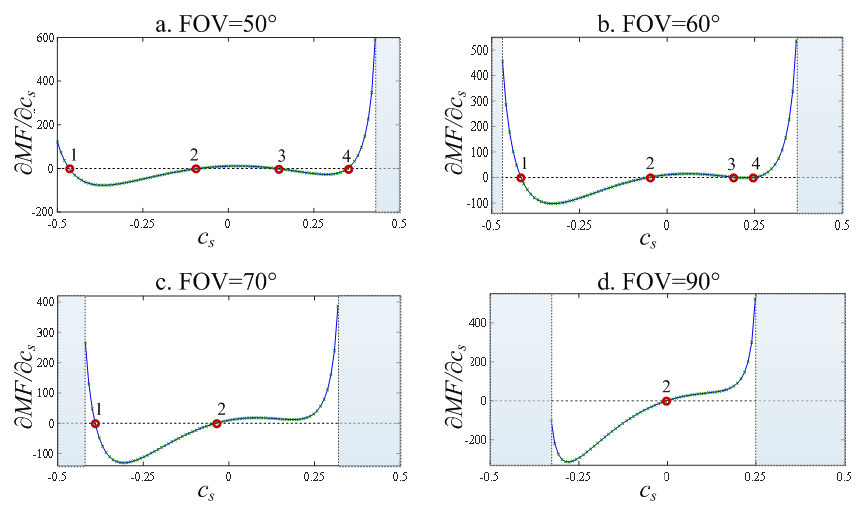
\includegraphics[width=.85\textwidth]{chapter-3/figures/PhaseTransition_field.png}
    \caption{SPC scan curves for different values of the FOV. Shaded areas are ray failure regions. The scan curves are obtained in the same way as the one shown in Figure \ref{fig:SPCscan}. Saddle point curvatures are marked by red circles. With the increase of the FOV, saddle point 1 disappears in the ray failure region. SP3 and SP4 merge with the minimum between them, and are replaced by a saddle point (not shown) that is not constructible with SPC.}
    \label{fig:phasechange_field}
\end{figure}

A different kind of change is also observed. At 50° [Figure \ref{fig:phasechange_field}(a)] four saddle points can be found. However, at larger fields the third and fourth saddle point first move closer [Figure \ref{fig:phasechange_field}(b)], merge and then disappear [Figure \ref{fig:phasechange_field}(c) and (d)]. 

By optimizing from the saddle points, at 50° it is found that the last two saddle points lead on one side of the saddle to the same minimum. While changing the FOV in small steps, it is possible to keep track of the two saddle points and one minimum by keeping the norm of the gradient to zero via minimization. The process is elaborated in Figure \ref{fig:systemdie}. When the FOV increases from 50° to 60°, it is seen that the Euclidean distances between the saddle points and minimum reduce. Hence the critical points are getting closer in the high-dimensional design space. At 70°, it is no longer possible to find saddle points via an SPC scan. However, it is still possible to obtain the merged point by keeping the norm of the gradient to zero at the vicinity of the previous critical points. From Figure \ref{fig:systemdie}, it is seen that the original two saddle points and one minimum merge into one saddle point with a merit function value of 74.92. It is a saddle point without any null elements, hence it cannot be constructed using SPC. This shows how two saddle points and one minimum merge into one saddle point while the FOV increases. 

\begin{figure}[h!]
    \centering
    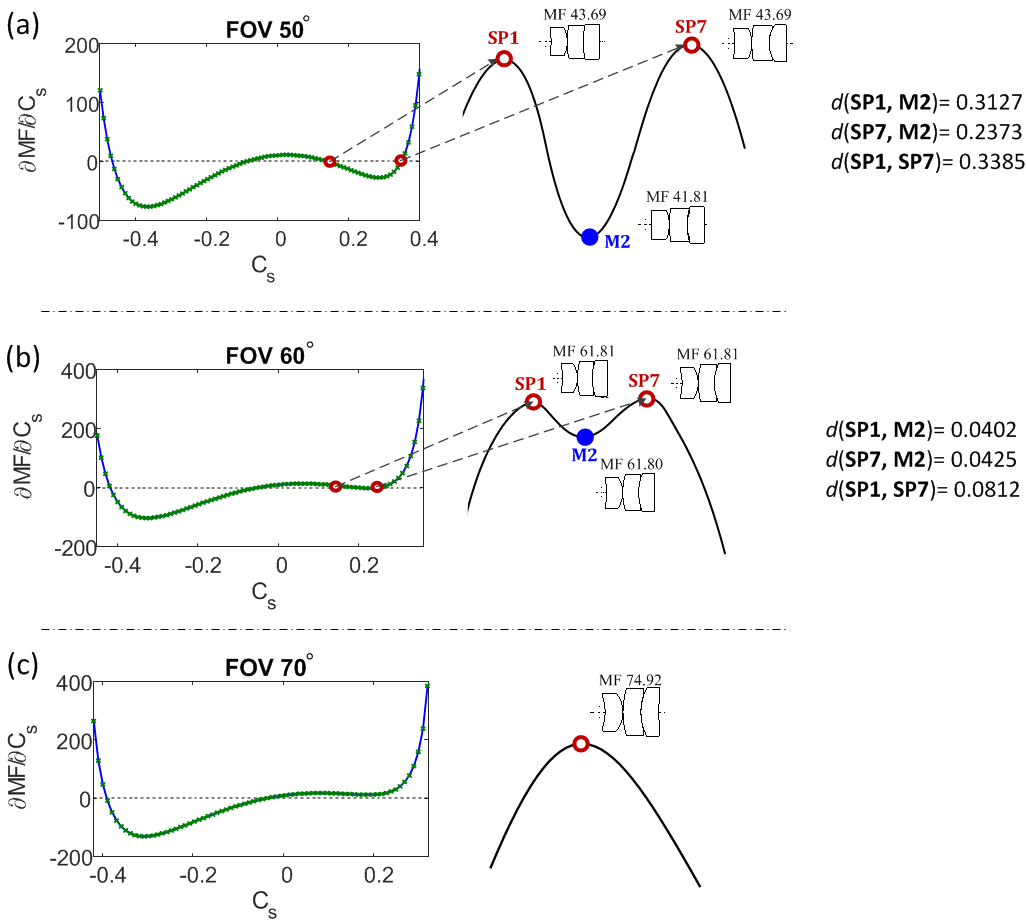
\includegraphics[width=0.8\textwidth]{chapter-3/figures/SystemDie.png}
    \caption{Merging of two saddle points and one minimum when the FOV increases, from Figure (a) to Figure (c). In the SPC scan curves, the two saddle points get closer and then disappear. The two saddle points and one minimum in between merge into one SP. The decreasing Euclidean distances also indicate the merging.}
    \label{fig:systemdie}
\end{figure}

A different phenomenon is observed when FOV increases. In Figure \ref{fig:systemborn}, the two saddle points on the left side of the scan curve are investigated: at 54°, SP8 and SP2 both lead to M9 when optimizing on one side. However, when the FOV increases to 56°, the two saddle points are connected to M3 instead of M9. The minimum M9 is connected to M3 via SP12. M3 and SP12 do not exist when the FOV is 54°. We see that when the FOV increases, a pair of local minimum (M3) and saddle point (SP12) start to emerge. Their merit function values are very close to each other (54.06 vs. 54.07) at 56° FOV. When the FOV increases to 60°, the difference between merit function values increases (61.31 vs. 61.96) as well as the Euclidean distance between M3 and SP12 (increases from 0.1148 to 0.2611). 

Besides merging or splitting, it is also found that in some special situations, when the FOV increases, both approaching and distancing\footnote{When mentioned merging, we observed that a pair of points approach each other and reach a situation where they cannot be distinguished anymore. When mentioned splitting, we observe that one point splits into two and they move away from each other. When this happens in a continuous way with a change of the system setting (e.g. FOV), approaching and distancing is used to describe the behaviour of the two points.} happens for the same pairs. Figure \ref{fig:systemreborn} illustrates a scenario when a glass null element was used as an SPC scan element. The FOV is increased from 60° to 110°, where three steps (60°, 90° and 110°) are plotted in the figure. At 60°, two saddle points were found by the scan. Both of them lead to a common minimum at one side (illustrated on the right of the scan curve). With the increasing of the FOV, the two saddle points become closer in the design landscape: the Euclidean distance reduces from 0.0785 to 0.0023 when the FOV increases from 60° to 90°. At this phase, a much smaller step size of the scan is necessary to be able to find the saddle point. After the FOV increased to 110°, the Euclidean distance between the two increases from 0.0023 to 0.0217. As a result, the tendency of the merging of the two saddle points changes to splitting. 

It is seen in the aforementioned three examples that the change of the design landscape can be dynamic and unpredictable. When a certain design specification changes, it essentially alters the design landscape. This change may affect the number of saddle points and minima which can be obtained with the SPC approach. Nevertheless, for the given examples, redundancy of the saddle point - minimum links also reduces the risk of missing solutions with the SPC approach. All the good solutions were obtained with the SPC method.

\begin{figure}[h!]
    \centering
    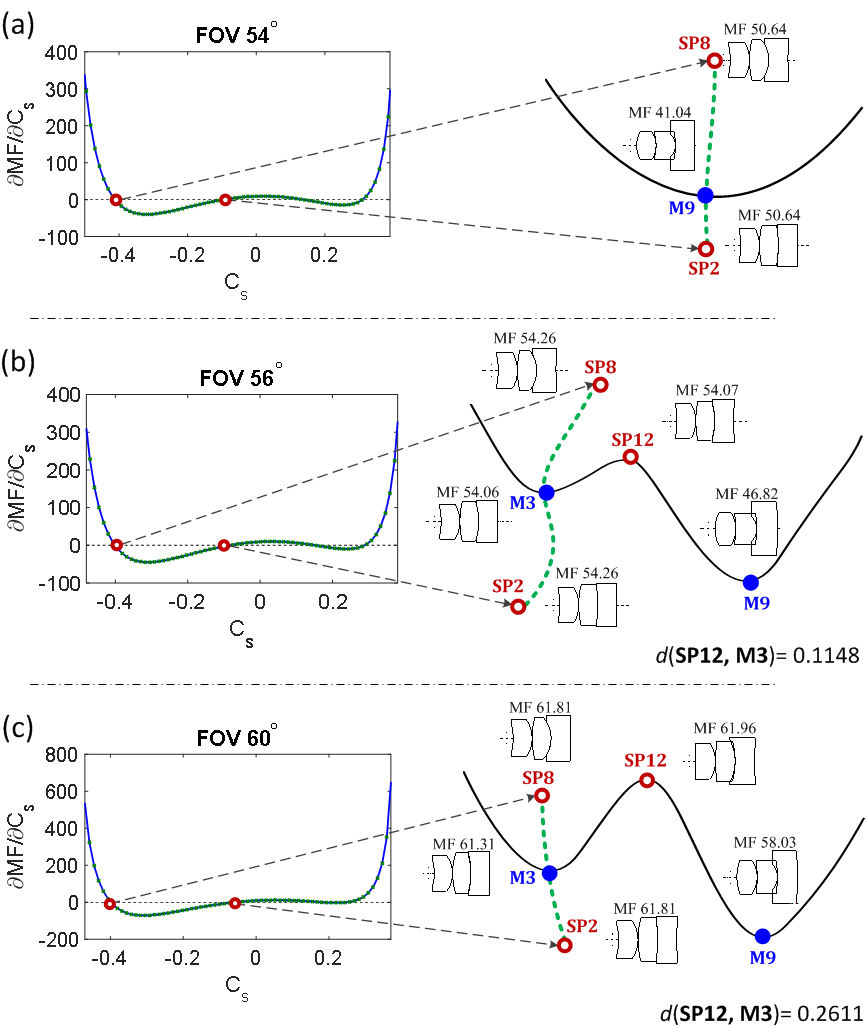
\includegraphics[width=0.75\textwidth]{chapter-3/figures/SystemBorn.png}
    \caption{A pair of minimum - saddle point emerges when FOV increases. From (a) to (c), the FOV increases. M3 and SP12 start to appear and form the link M3-SP12-M9. The connection between saddle points and minima are altered: at 54°, SP8 and SP12 connect to M9; at 56°, SP8 and SP12 connect to M3.}
    \label{fig:systemborn}
\end{figure}

\begin{figure}[h!]
    \centering
    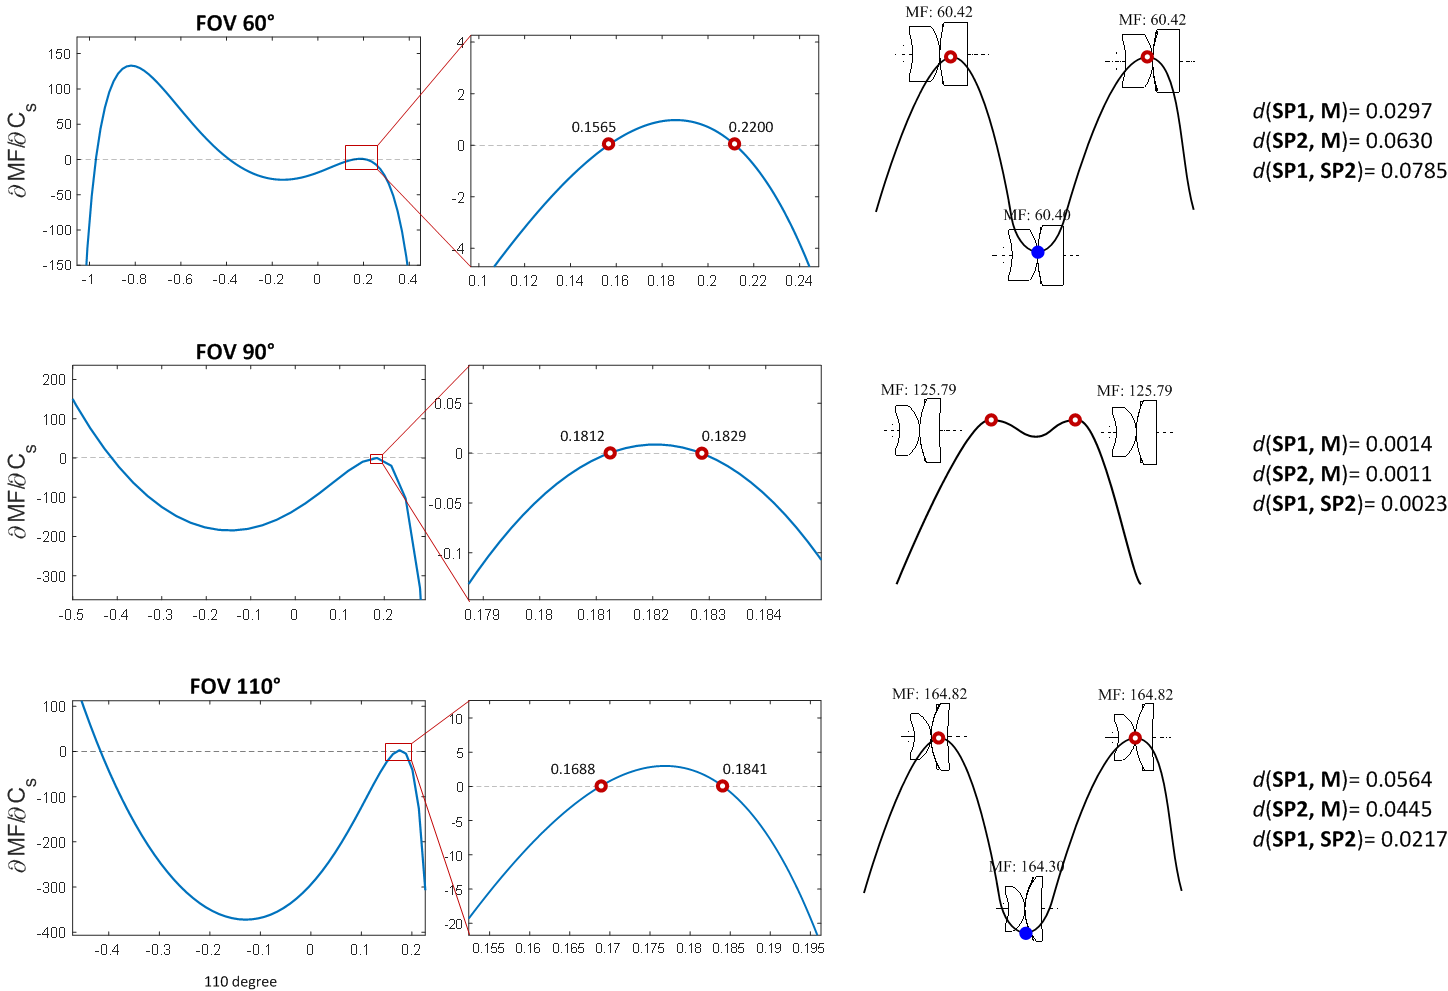
\includegraphics[width=0.8\textwidth]{chapter-3/figures/SystemReborn_vt.png}
    \caption{A glass null-element SPC scan is performed on DB-M1 from Figure \ref{fig:single2double}. The scan position is between the two lens elements. When the FOV increases from 60° to 110°, the two saddle points on the right first get closer, and then further apart. This phenomenon can be observed from the SPC scan curve as well as from the Euclidean distances between the two.}
    \label{fig:systemreborn}
\end{figure}
%%%%%%%%%%%%%%%%%%% Section %%%%%%%%%%%%%%%%%%%%%%%%%%%%%

\section{Discussion and Conclusion}
The design landscape of a wide-angle pinhole lens and its closely related optimization landscape are investigated in this chapter. Several observations that result from this study have a more general validity. Switching between minima with SPC introduced in Subsection \ref{cp2-switching}, is applied to the pinhole lens as shown in Figure \ref{fig:wideangleSwitch}. It can be used in other design tasks as well to avoid the trapping of the optimization in a sub-optimal solution. Combining SPC with conventional design methods, as shown in Figure \ref{fig:WideAngleDesign}, can lead to good complex designs starting from simpler ones \cite{LivshitsSP2014}.

The lens design landscape is different from general global optimization problems because of the close relationship that often exists between the local minima of a design problem and local minima with one lens less. Figure \ref{fig:tripletnetwork} is particularly useful to illustrate this structure, due to the special choices that are made in the corresponding search (lenses in contact, use of air null elements). The systems SP1–SP11 are triplet saddle points, but if the air null-element of the corresponding scan (a pair of surfaces that has no influence at all on the rays or on the merit function) is removed, they become doublet minima. However, when these doublet minima with an extra null-element are optimized on both sides of the resulting saddle, they lead to the triplet minima M1–M10. In the search shown in Figure \ref{fig:tripletnetwork}, these 10 triplet minima are all minima found in the landscape with other methods such as NETMIN and CODE V that are used for comparison. A scenario where this structure holds for all minima has been previously encountered \cite{PascalTriplet2009}. The corresponding landscape is dominated by spherical aberration. The wide angle examples discussed here show that the scenario where this structure is present for most of the minima, can be much more general.

% HZ: the structure is a structure that all minima are connected via saddle points, and these saddle points can be constructed using SPC. Having a trans-dimensional structure of the minima and saddle point does not ensure the connection of the saddle point and minima within the same dimension. Local or global structure?

The example shown in Figure \ref{fig:tripletnetwork} has the advantage that the special structure can be observed in a pure form, where all minima and saddle points are connected and the saddle points can be constructed using SPC. Interference of other features can also be present as seen in the examples: Figure \ref{fig:thicknesschange} indicates that some minima do not have a corresponding system with a zero-thickness element, therefore cannot be obtained following the SPC procedure; Figure \ref{fig:phasechange_field} shows that saddle points which cannot be constructed with SPC are present. In these examples, using SPC cannot always find all minima. Nevertheless, Figure \ref{fig:TripletMonoNetwork} shows an example where even in the presence of the aforementioned features of the landscape, the five solutions with the lowest merit function value found with other methods can still be found with SPC.

The example shown in Figure \ref{fig:phasechange_field} is useful for understanding the transition in the local landscape where saddle points that can be constructed using SPC become ones that cannot be constructed using SPC. In an extreme case where none of the saddle points can be constructed using SPC, the landscape becomes a standard global optimization landscape which does not have the special structure we mentioned. The replacement of the SP3 and SP4 in Figure \ref{fig:phasechange_field} by a saddle point, which cannot be constructed with SPC, shows that the landscape is locally transformed into such a standard global optimization landscape. The process is elaborated in Figure \ref{fig:systemdie}. However, the transition can also happen in the opposite direction if the process (in this case, descreasing the FOV) is reversed: a usual saddle point splits into two saddle points and a minimum in between, and in this case, the two saddle points can be constructed using SPC. This complexity of the design landscape dynamic is further explored in Figure \ref{fig:systemborn} and Figure \ref{fig:systemreborn}: When the FOV is increasing, a pair of minimum - saddle point appears; Two saddle points and a minimum first tend to merge and then tend to separate again. 

Based on the examples shown in this chapter, the complex dynamic of the design landscape can already be observed. However, the structure that enables SPC to obtain good solutions is stable. For systems that are more complex than those presented in this chapter, the utility of SPC will be determined by its practical success, rather than by a detailed study of the entire landscape, which becomes difficult. Systems with bigger complexities are investigated in the next chapter. 

The replacement of high-dimensional searches by several one-dimensional searches plus local optimization can lead to a reduction of the complexity of the search. It can be essential for practical purposes. Compared to global optimization methods where multiple starting points are firstly chosen heuristically and then local optimization is applied, SPC operates in a more systematic way that starting points are provided based on constructed saddle points. In computer programs where the search for new solutions is automated, the general version of SPC could be combined with other methods. In the case of the special version of SPC this has already been achieved in the commercial software SYNOPSYS \cite{DilworthSP2012}. Excepting simple problems, no known global optimization method can guarantee finding all (good) solutions in a reasonable time, and SPC is no exception. However, high-quality designs have already been obtained with the special \cite{MarinescuSP2008}\cite{BociortPatent2010} and with the general versions \cite{LivshitsSP2014} of SPC. SPC will finally be validated if many high-quality designs are obtained with this method.

%We have seen that in lens design we can find good solutions with SPC. This method could also be applicable in other design problems where the conditions described in Sections 3 and 4 of \cite{MVTurnhoutSPC15} or in the Appendix of \cite{BociortToyModel2010} are satisfied. In a different multi-parameter optimization problem, if there is a way to construct a
%saddle point in the design landscape, then in principle, it should be possible to follow the same procedure as in lens design to search for new solutions.


\references{dissertation}


\chapter{Applying SPC in Complex Systems} %% change
\label{chapter_4_complex_system_exploration} %% change
\graphicspath{ {./chapter-4/figures/} }  %% change
\captionsetup[figure]{labelfont=bf}
\captionsetup{margin=1.5em}
\captionsetup[table]{labelfont=bf}

%%Newdefined commands
%for circled number typing
\newcommand*\circled[1]{\tikz[baseline=(char.base)]{
            \node[shape=circle,draw,inner sep=0.5pt] (char) {#1};}}

% The following annotation is customary for chapter which have already been
% published as a paper.
\blfootnote{Parts of this chapter were presented in the SPIE conference Optical Systems Design (2018, Frankfurt) and published in Proc. SPIE \textbf{10690}, Optical Design and Engineering VII, 1069007 (2018) \cite{ZheHOU2018OSD}.}

%% The '0pt' option ensures that no extra vertical space follows this epigraph,
%% since there is another epigraph after it.
\epigraph[0pt]{
If you cannot measure it, you cannot improve it\footnote{The quote is popularly rephrased from the original quote "When you can measure what you are speaking about, and express it in numbers, you know something about it; but when you cannot measure it, when you cannot express it in numbers, your knowledge is of a meagre and unsatisfactory kind: it may be the beginning of knowledge, but you have scarcely, in your thoughts, advanced to the stage of science, whatever the matter may be."}.
}{Lord Kelvin}

% \epigraph{
%     Sample quotes
% }{author}

% \begin{abstract}
% Previous researches have shown that different solutions of the optical system can be found using saddle point based method for some simplified cases\cite{PascalTriplet2009}. It is important, however, to study whether the saddle point based method still perform well in practical lens design problems. To study this, we chose to start with a relative simple example.
% \end{abstract}

% %% Start the actual chapter on a new page.
%newpage
\vspace{2em}

In Chapters \ref{chapter_SPC_method_reccomendation}  and \ref{chapter_SPC_simple_system_landscape}, suggestions are given on how to apply SPC to simple design problems. In this chapter, SPC is applied to some more complicated practical design problems.

%%%%%%%%%%%%%%%%%%%%%%%%%%%%%%%%%%%%%%%%%%% Section 1 %%%%%%%%%%%%%%%%%%%%%%%%%%%%%%%%%%%%%%%
\section{Introduction}
For a simple optical design system, such as a doublet or a triplet, the number of variables is rather small. It is possible to use different design (optimization) strategies (including SPC) to search for all or most of the local minima. So for these relatively simple systems, the results produced by SPC can be compared with those produced by other methods. This was done in Chapter \ref{chapter_SPC_simple_system_landscape}, where the design network of a simple wide-angle pin-hole lens \cite{HouSimple16} shows that SPC is effective in escaping from poor local minima and reaching the best minimum. In a specific case, SPC is able to find all the solutions found in the design landscape that other methods also find. The number of variables used in this study was five (only curvatures). However, in a practical problem where a larger number of variables is used, it is difficult to successfully repeat a similar study. One of the reasons is that the number of local minima increases dramatically with the number of variables. It is not possible to find every minimum in a complex design landscape, hence, also less meaningful to compare the results obtained with different methods.  

%"Proof of the pudding is in the eating." 
Despite the preceding observations, the SPC method can be applied in a complex lens design problem. Attempts have been made to apply the special version (Chapter \ref{SPC_Special}) of SPC to some complex objective designs\cite{OanaOEngPart2}\cite{CaoCatadioptricwithSPCOeng2017}, and the results of general version (Chapter \ref{SPC_general}) has also been shown to produce good systems\cite{LivshitsSP2014}. However, in all cases, the details of how SPC should be applied effectively is not explained, therefore it is difficult to quantify the performance of the method, and reproducing the same results from the mentioned studies is not possible. 

In this chapter, we derive recommendations for how to apply SPC to several practical design problems, namely: 1) a wide-angle system consisting of two groups of lenses where SPC can only be used for a limited number of positions in the system; 2) two microscope objectives, where designer experience and SPC produce additional solutions; 3) a complex lithographic objective where applying SPC shows improvement in the intermediate design stage. 


\section{Investigation of a Wide-angle Lens with Six Elements}
Wide-angle lenses are broadly used in various applications, including photographic cameras, surveillance cameras and projectors. To increase the field of view of an optical system and while maintaining an image of good quality, a certain amount of complexity of the system is necessary. We consider here a wide-angle lens with a moderate complexity to study the performance of SPC as an approach to switch between solutions with the same number of variables. The system consists of six lenses including one cemented surface. There are eleven surfaces, hence eleven variables in terms of curvatures. The design specifications of the lens are shown in Table \ref{table: sysspecWAL} and the surface specification is available in Appendix \ref{apdx: wide-angle-specs_6_elements}. The maximum field of view is 120°. The overall length of the system is 38.75mm, which is small enough for integration into surveillance systems. The Modulated Transfer Function (MTF) curve shows that the modulation stays above 0.4 for 100 cycles/mm at full field of view (\ref{fig:wideanglelensPerformance}). The system is not optimized for distortion which can be corrected with image processing afterwards (e.g. digital dewarping \cite{Sahin:18DisCorrec}).



\setlength{\arrayrulewidth}{.5mm}
\setlength{\tabcolsep}{18pt}
\renewcommand{\arraystretch}{1.2}
\begin{table}[h!]
    \centering
    \captionsetup{justification=centering}
    \caption{System specification of the wide-angle lens}
    \label{table: sysspecWAL}
    \vspace{-1em}
    \begin{tabular}{ p{20em} c }
    \hline 
    Full Field Of View (°) & 120\\
    Effective Focal Length (mm) & 3.0\\
    F Number & 2.0\\
    Overall Length (mm) & 38.75\\
    Wavelength (nm) & 644, 546, 480\\ %(e, F', C')\\
    \hline
    \end{tabular}
\end{table}

\subsection{Design a Wide-angle Lens with SPC}

The wide-angle lens is first designed with a conventional method by using surfaces with special properties (concentric and aplanatic) \cite{LivshitsQA2013}. Surfaces, at which the chief ray has everywhere a normal incident angle, are free from coma and astigmatism. In what follows we will call such an optical surface a concentric surface. The aplanatic surfaces in the system do not introduce spherical aberration and coma. In the system plot of Figure \ref{fig:wideanglelensPerformance}, it is shown that the six lenses are divided into two groups. A front group with three lenses is responsible for expanding the field of view. A rear group containing a cemented element is the focusing group. The two parts of the system were first designed separately and then combined to form the complete lens system. To combine the two parts, the front group has the stop at the end of the lens group, and the rear group has the stop in front of it.  The front group is designed as an afocal system with an angle reduction ratio of 0.3. The field of view on the object side is designed to be 120° and the field of view on the image side is 40°. The rear group is designed as a focusing system with a field of view of the same 40°. The diameter of the common stop of the two parts, which is the aperture stop of the whole system, is 4.5 mm. 

\begin{figure}[h!]
    \centering
    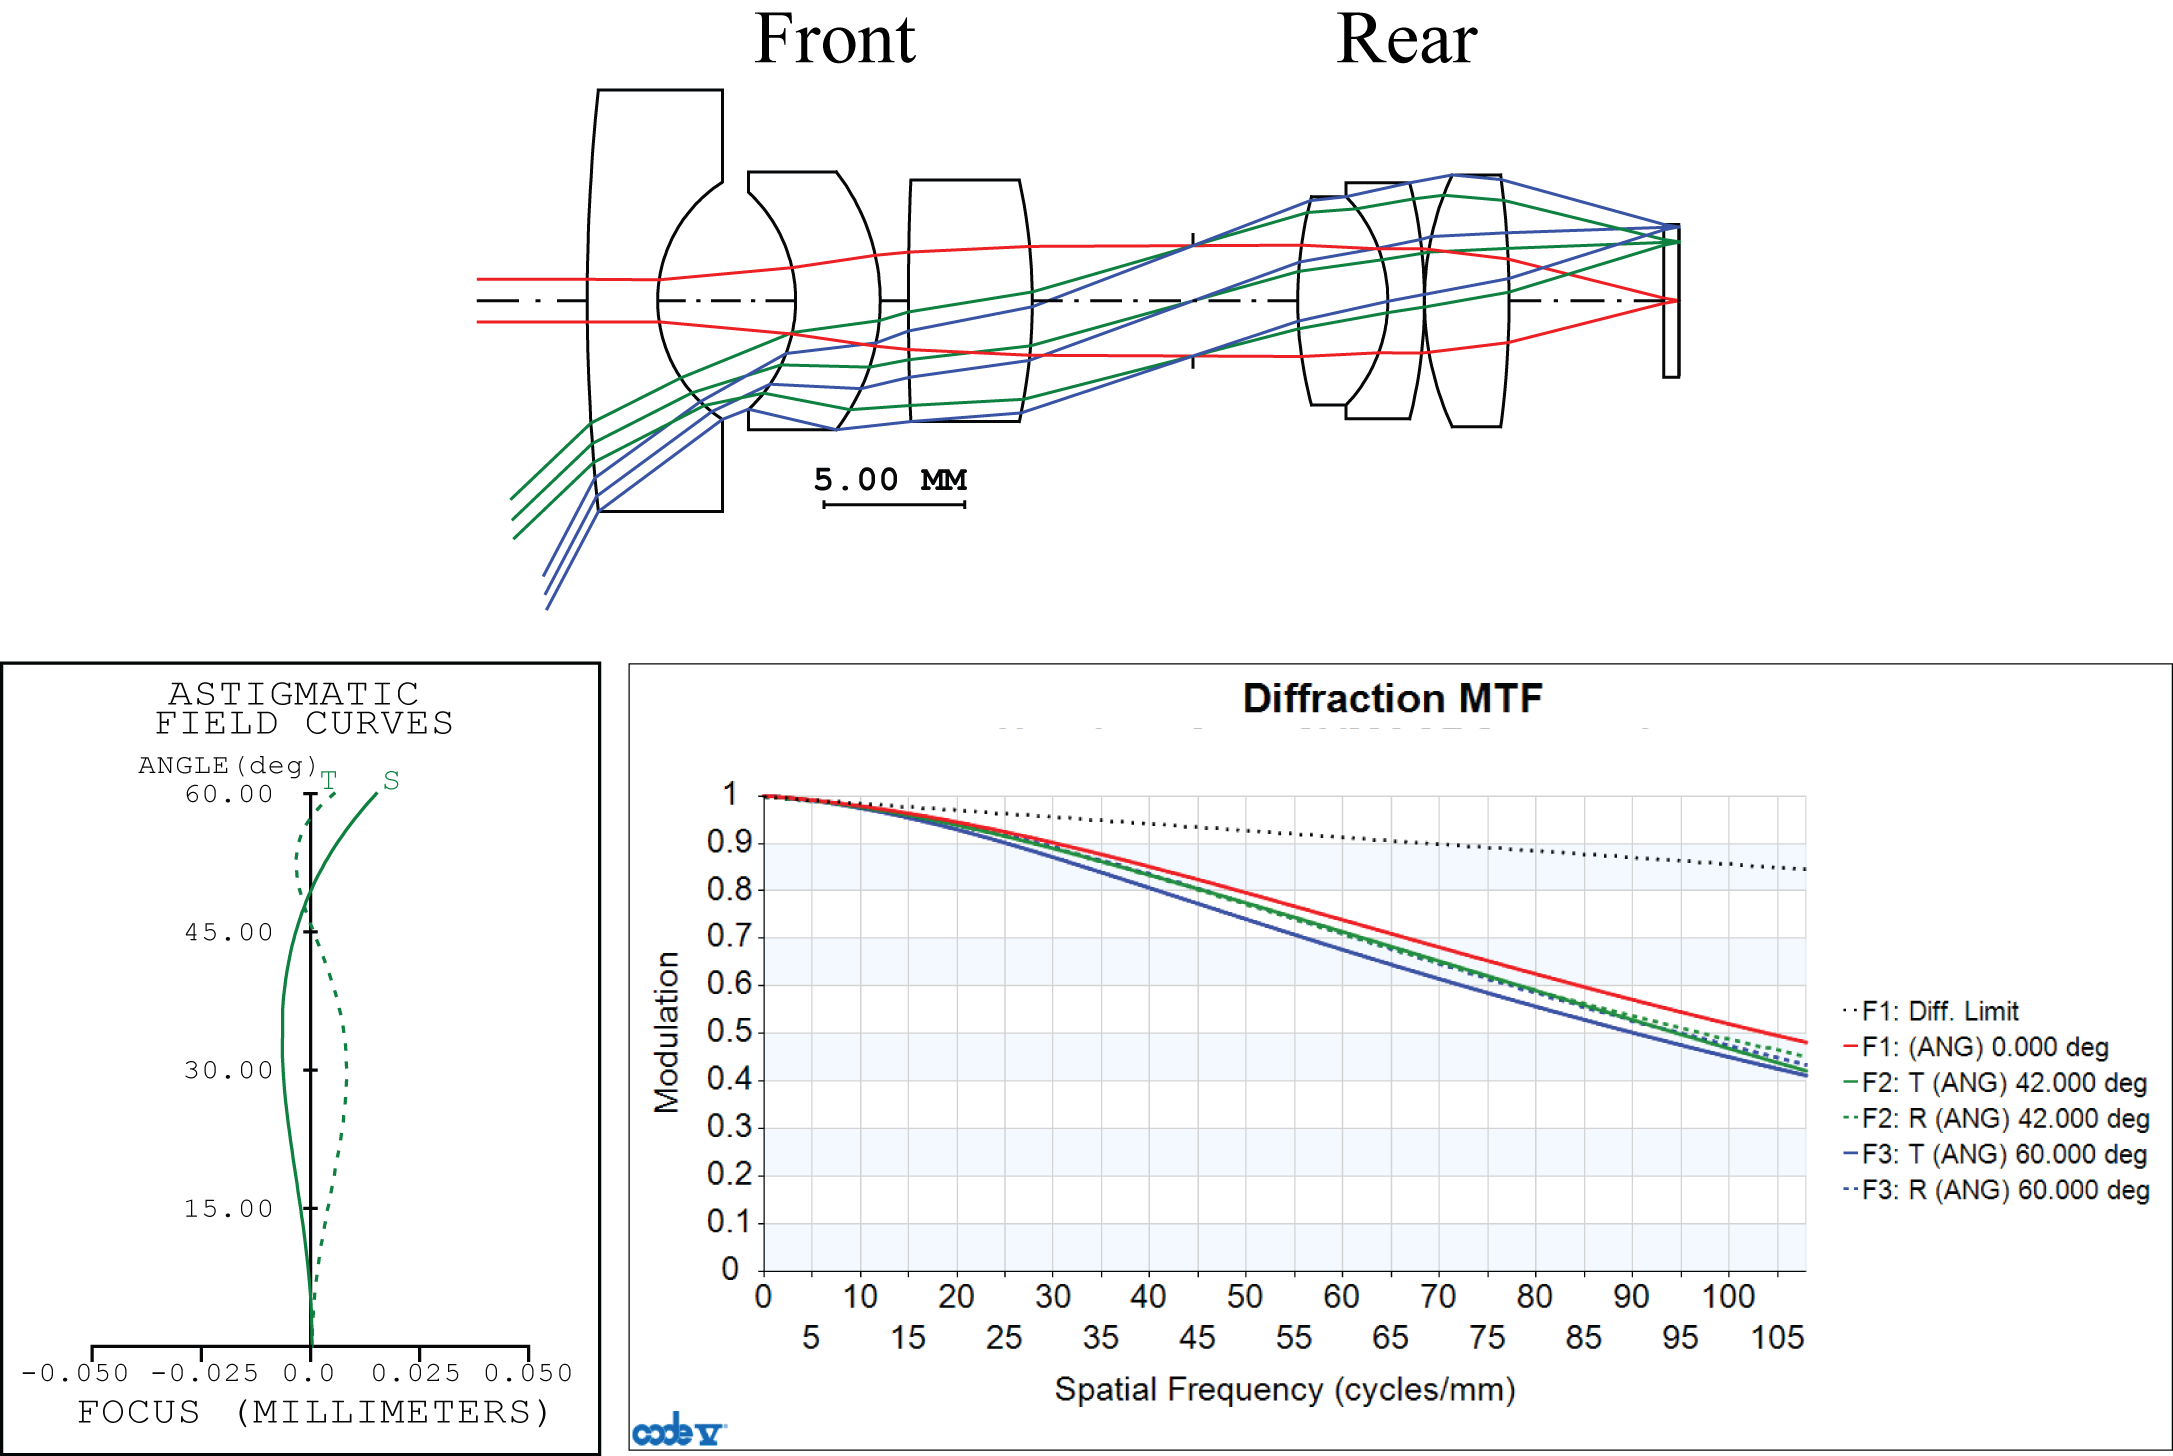
\includegraphics[scale=0.68]{chapter-4/figures/WideAngleL.png}
    \caption{System plot of a wide-angle lens and its performance.}
    \label{fig:wideanglelensPerformance}
\end{figure}

With the conventional method, the design of the front group started with a single lens using a flat and a concentric surface, given that the stop is at the right side of the lens. A moderate field of view is first used. Then lenses are added with either concentric or aplanatic surfaces. Adjustment and optimization are done to increase the field of view and achieve an angle reduction ratio of 0.3. The curvatures and thickness are both optimized. The rear group is designed separately by starting with a cemented flat surface doublet and two concentric surfaces. Another lens is added and a different glass is used to further reduce the monochromatic and chromatic aberration. The front group and rear group are then combined to optimize for the final solution.

When a solution is obtained by the conventional approach, SPC can be used to investigate alternative solutions. Since the system is combined from two separate parts, one way is to apply SPC to both the front and rear parts alone, without the other part being present. After that, different combinations of the front and rear parts can be investigated. Another way of applying SPC is to search for new solutions for the combined system.

After applying SPC to the front group and rear group alone, we obtain one solution for the front group and three solutions for the rear group. The next step is to combine the front group option with the rear group options. This is done by connecting the two groups and performing an optimization with the curvatures. All three cases provide the same final solution as illustrated in Figure \ref{fig:WAL_combine}.

\begin{figure}[h!]
    \centering
    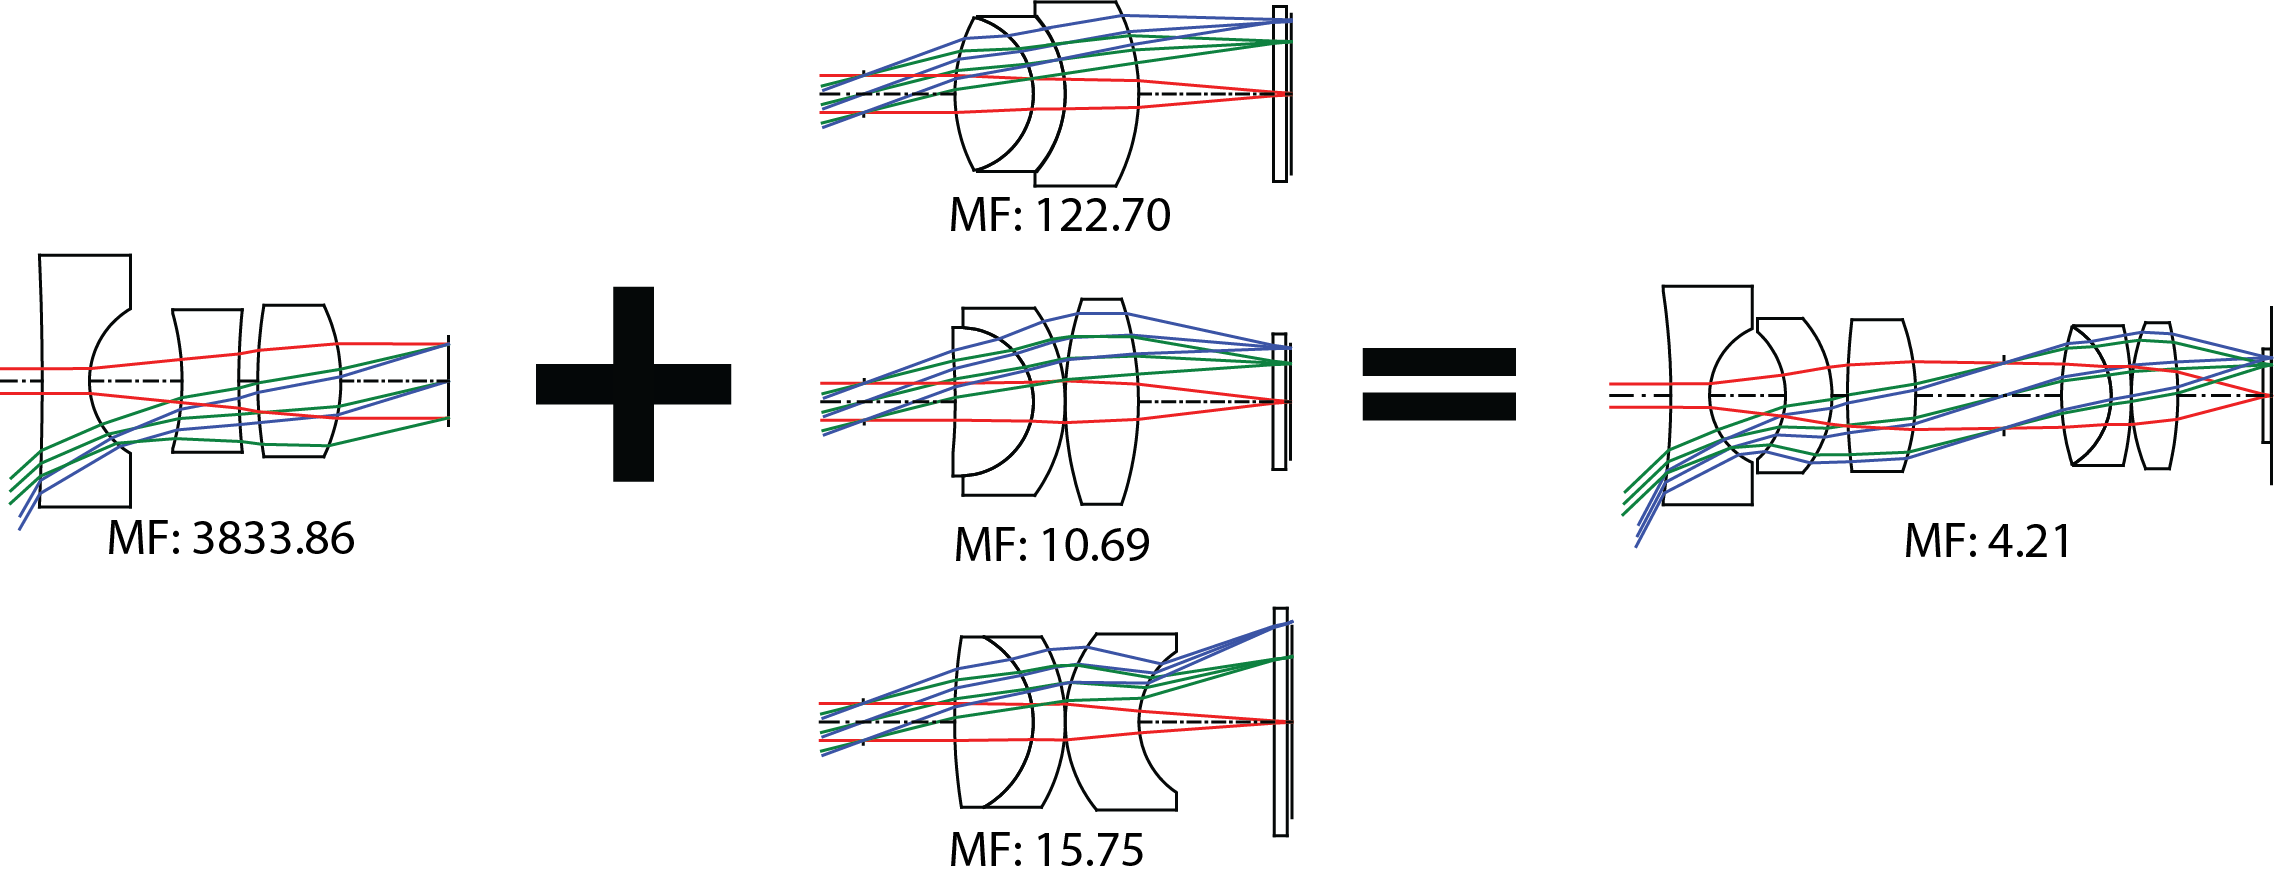
\includegraphics[width=0.7\textwidth]{chapter-4/figures/WAL_combine.png}
    \caption{Combinations of the front part (conventional approach) and the three rear parts (conventional with SPC). All converged to one solution. Merit Function (MF) values of the systems are provided. }
    \label{fig:WAL_combine}
\end{figure}

Once the combined system is obtained, SPC is performed to search for alternative solutions with the same amount of variables. As explained in Chapter 3, the first step is to extract lenses from the original system. Because the first lens is responsible for collecting the large angle rays, extracting it from the system while keeping the large field of view is not possible. The only possible lenses to extract and perform SPC scans are the second, third and last elements. The current SPC cannot be performed on cemented elements for switching to a different solution. It is because a cemented lens requires the two sub-elements to be in contact (having a shared surface). A null element cannot be created in such a situation while varying the curvatures for the SPC scan. The merit function based on transverse aberration in CODE V is used in this example. It is a composite value, scaled so that it is the mean square of the weighted image radius (unit: \textmu m$^2$). We keep the paraxial marginal ray exit angle as $-0.25$ rad on the last surface to ensure that the effective focal length is equivalent to $3.0$ mm (the entrance pupil diameter is 1.5 mm). Ten curvatures are used as variables. Six different minima are found in the design network illustrated in Figure \ref{fig:WAL_network}. A global optimization run (Global Synthesis of CODE V) is also performed. No additional local minima are found compared to the result of SPC. From Figure \ref{fig:WAL_network}, it is noticed that the major difference in the systems are in the front group. The system shape stays the same for the rear group in all six solutions.

The relationship between different systems is indicated by arrows in Figure \ref{fig:WAL_network}. Black arrows show that via SPC, two systems are connected in both ways. If M1 and M2 are connected in both ways, it means that by using SPC, M2 can be found starting from M1, and vice versa. Blue arrows indicate a one-way connection. For example, starting from M2, it is possible to find M3 via SPC. However, M3 does not lead to M2 by using SPC. Normally, the expected situation is a two-way connection. However, a one-way connection can appear in two scenarios: In the first scenario, a system with high stress and higher value of merit function is unstable (e.g. M6). The stability indicates the size of the basins of attraction. An unstable local minimum has a relative smaller basin of attraction compared to others. Therefore, it is easy to get out of this kind of poor local minimum with SPC. However, it is not easy (and not necessary for practical purposes) to reach them. The second scenario happens when two minima are very close to each other in the design space (e.g. M1 and M2). The landscape has relative smaller variation in this region around the two close minima. In Figure \ref{fig:WAL_network}, systems M1 and M2 (best two systems) have similar system shapes and close values of the merit function. Another system, such as M3 or M4, obtained by switching from M2, can easily, when switched back, go to M1. 

As shown in Figure \ref{fig:WAL_network}, all minima are connected within one network. It means that starting from any of the minima in the network, there is always a route to reach any other system. It can also be observed that the less good solutions (M3, M4, M5, and M6) are all directly connected with best two systems (M1 and M2). This implies that if the design process was trapped in one of the poor solutions, applying SPC once would be sufficient to switch to one of best two systems.  

\begin{figure}[h!]
    \centering
    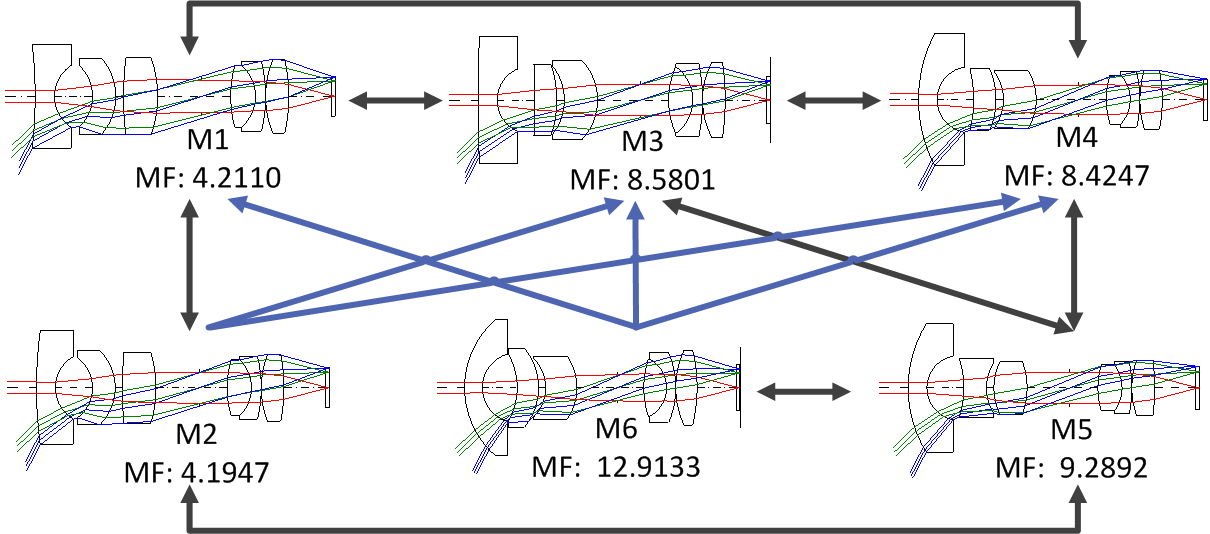
\includegraphics[width=0.8\textwidth]{chapter-4/figures/WAL_network.png}
    \caption{A network of minima for the wide-angle lens. All systems are connected with SPC. Global optimization using CODE V did not find additional systems. The transverse ray aberration in CODE V is used as the merit function.}
    \label{fig:WAL_network}
\end{figure}

\subsection{Stepwise Analysis of SPC for a Wide-angle System}
\subsubsection{Visualization of the Saddle Point }
In Chapter 3, recommendations have been given for applying SPC in steps. Examples are presented in this section to demonstrate how SPC is applied to the wide-angle system. The system M3 in Figure \ref{fig:WAL_network} is selected to demonstrate how SPC is practically performed. First, by extracting (details are described in Chapter \ref{cp2-switching}) the second element from M3, a minimum with one lens less is obtained. Then, a null element is inserted at the the same position where the lens is extracted and an SPC scan \ref{para: performing SPC scan} is performed on the null element. This null element is not in contact with the existing lens elements in front of or behind it.  With the SPC scan, curvatures of the null-element are chosen such that saddle point systems are obtained. Figure \ref{fig:WAL_demo_sp} shows the SPC scan curve (Figure \ref{fig:WAL_demo_sp}(b)) and the corresponding saddle point system (Figure \ref{fig:WAL_demo_sp}(a)) which is found by the scan. In an SPC scan curve, the crossing of the curve and the horizontal axis indicates the curvature of the saddle point system (the black dot in Figure \ref{fig:WAL_demo_sp}(b)). In this case, only one saddle point system is found via the scan and the curvature of the saddle point system is -0.170 $mm^{-1}$. 

The saddle point system obtained using SPC scan is usually a saddle point with a Morse Index of 1. This means that there exists a 2D plane in the high-dimensional design space where from the obtained saddle point, along one direction the value of merit function decreases, and along another (orthogonal to the previous one) the value increases. Given this 2D plane, the saddle point can be be visualized (Figure \ref{fig:WAL_demo_sp}(c)). 
\begin{figure}[h!]
    \centering
    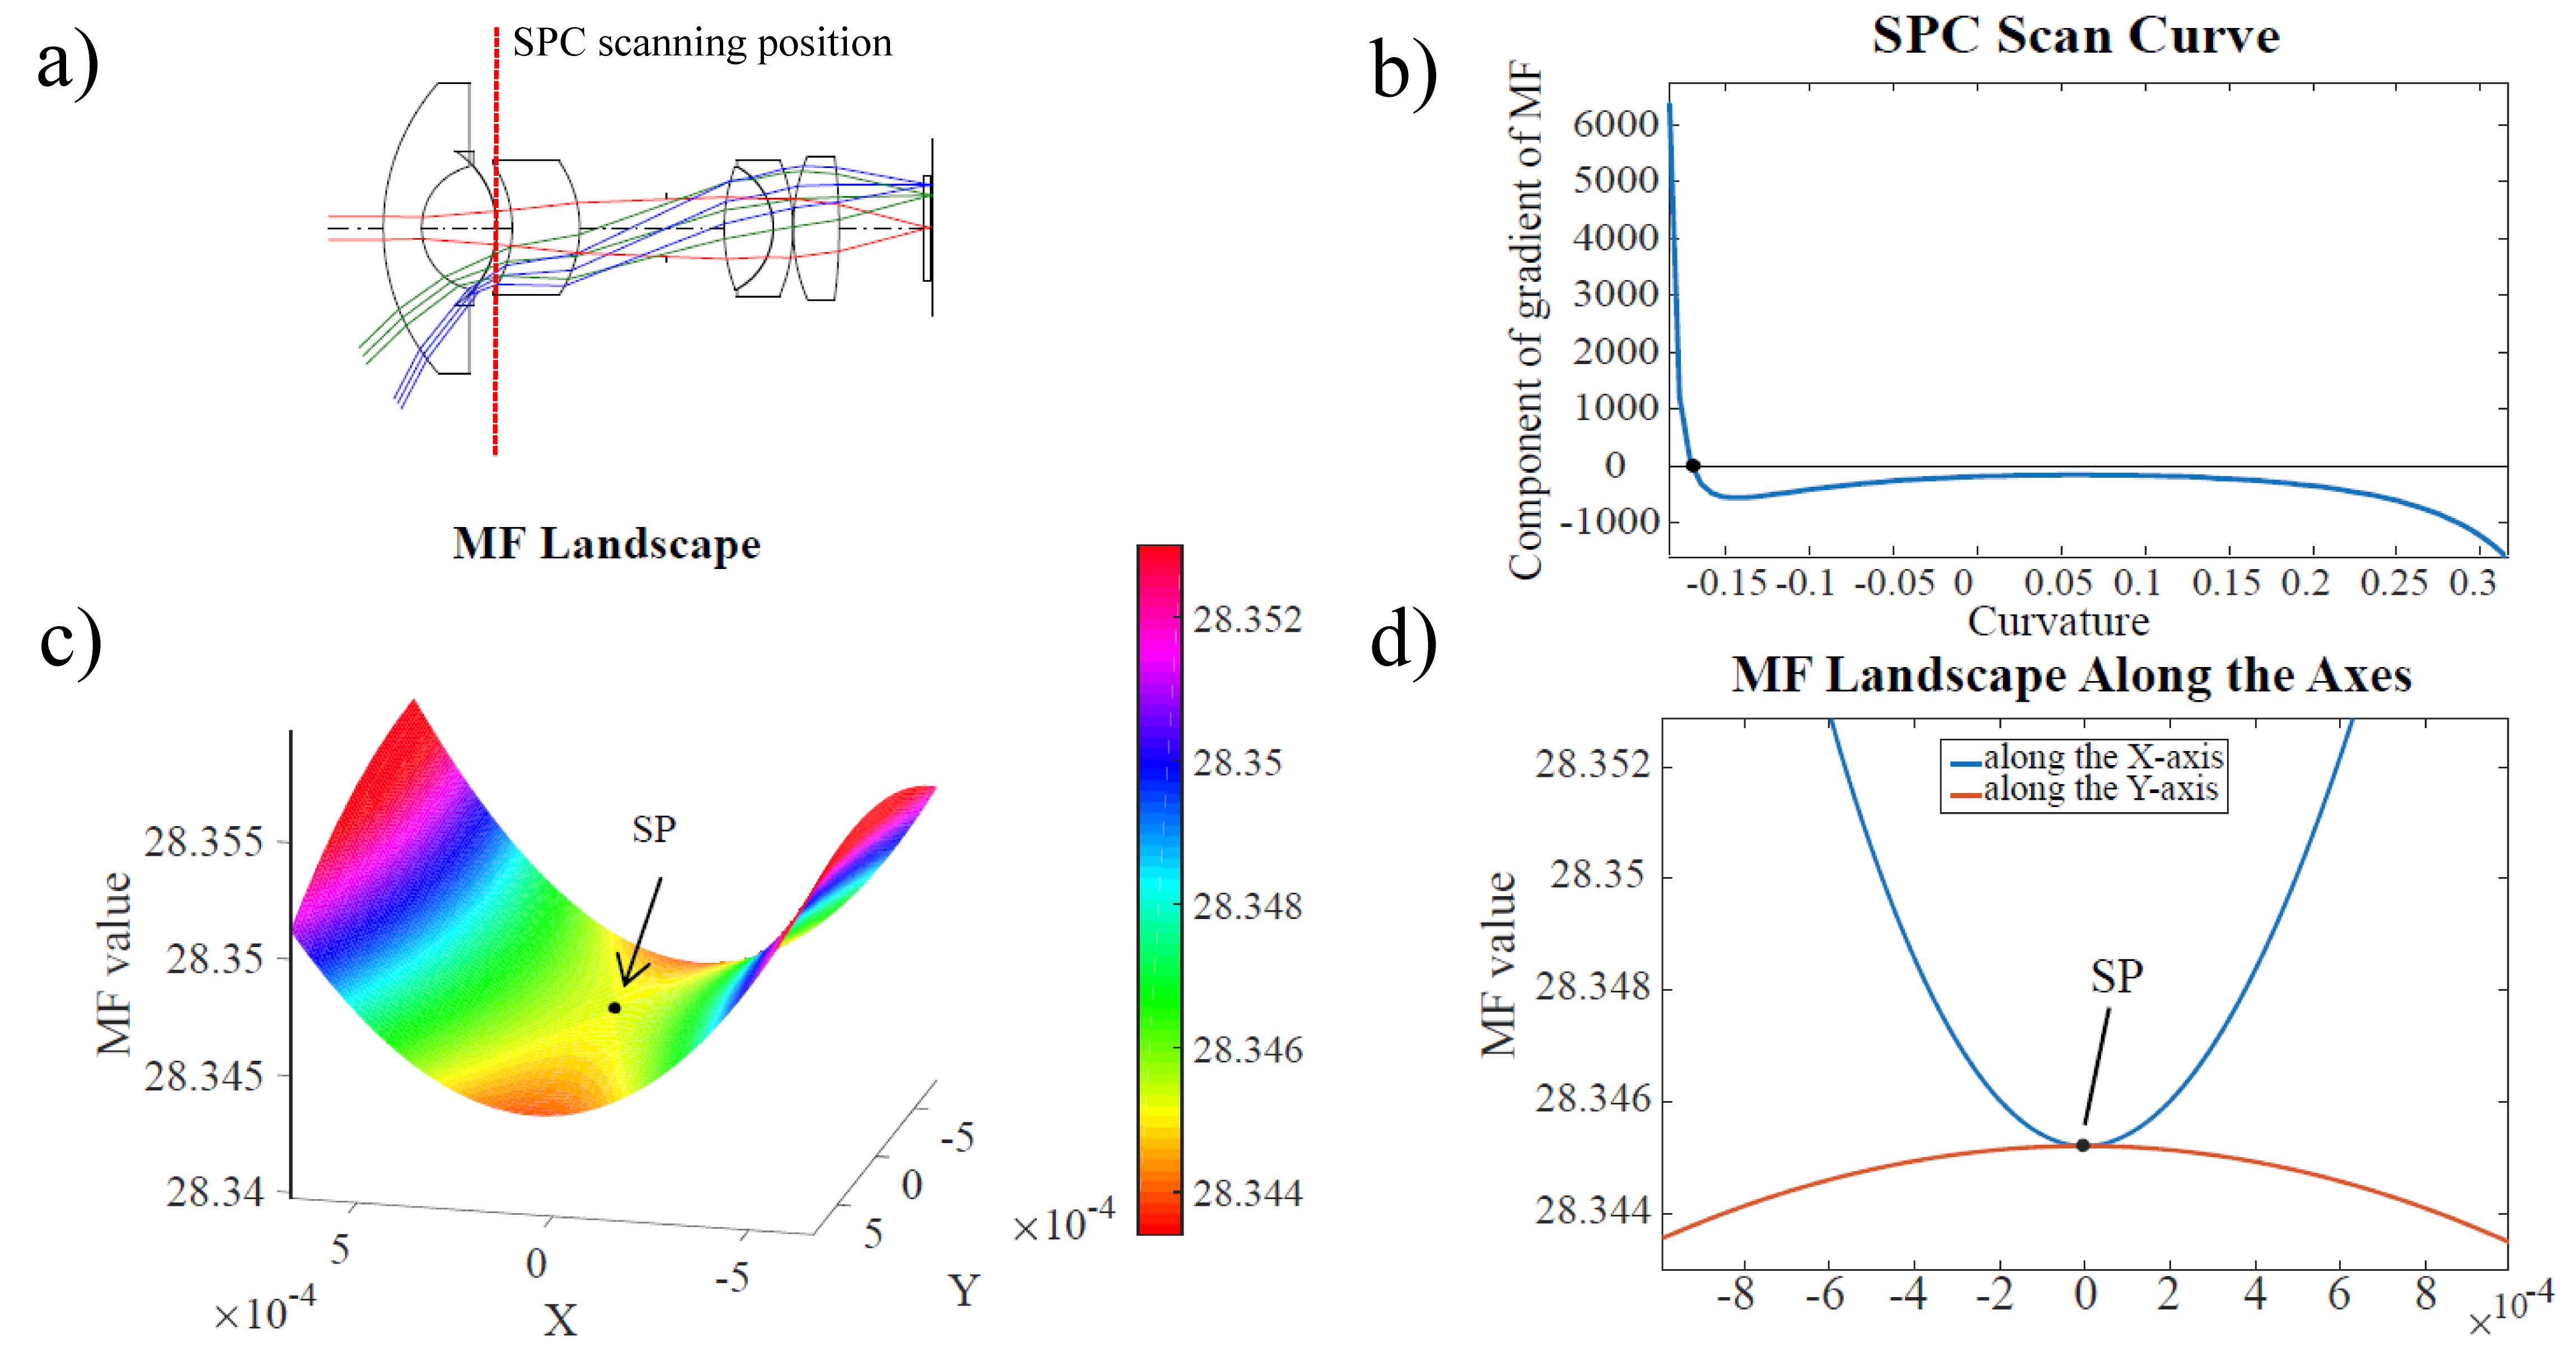
\includegraphics[width=\textwidth]{chapter-4/figures/WAL_demo_sp.png}
    \caption{a): the system we choose for the SPC scan. b): the SPC scan curve. c): the saddle point visualized in the chosen 2D plane (Figure \ref{fig:hyperplane}. d): the descending and ascending direction around the saddle point in the same 2D plane. The saddle point is marked with a black dot.}
    \label{fig:WAL_demo_sp}
\end{figure}

The value of the merit function for the saddle point equals the value of the merit function at the minimum before adding the extra two variables. If the direction where the merit function decreases can be determined, then the 2D plane to visualize the saddle point can be easily chosen. Numerically, this direction can be determined by minimizing on a hyperplane, which is orthogonal to the SPC scan line along which the merit function value is constant. In Figure \ref{fig:hyperplane}(a), we use a 3D case to demonstrate how such a hyperplane is found. The 3D space has the coordinates $(x_1, \eta, \xi)$. The variables are explained in Figure \ref{fig:hyperplane}(b): $x_1 = c_1$, where $c_1$ is the curvature variable which does not belong to the null element; $\eta = c_2 + c_3$, $\xi = c_2 - c_3$, where $c_2$ and $c_3$ are the curvatures of the null element.  Point $S (x_{1,m}, \eta_{s}, 0)$ is the saddle point system containing the null element. Point $A$ is a point on the line close to Point $S$ where the merit function value is constant. And the value of the merit function is the same as Point $S$. An example of the merit function landscape in the $x_1, \eta$ plane is given in Figure \ref{fig:hyperplane}(c). Along the line $SA$, the value of the merit function is constant, hence, to find the direction of descent in a $N$-dimensional space, we have to move in the $(N-1)$-dimensional hyperplane which is perpendicular to the line $SA$. It is the 2D plane $P1$ as shown in Figure \ref{fig:hyperplane}(a). On this plane, $B$ is a point where the merit function value is minimized. We will have $MF_{B}$ < $MF_{S}$. With points $A$, $B$ and $S$, a 2D plane $P2$ can be determined in which we can plot both the directions of ascent and descent . Given the two vectors on the 2D plane, $\overrightarrow{SA}$ and $\overrightarrow{SB}$, an orthogonal base can be calculated with the Gram-Schmidt process:

\setlength{\belowdisplayshortskip}{5pt}
\setlength{\abovedisplayshortskip}{5pt}
\begin{equation} \label{eq:u1}
\pmb{\beta_{1}} =  \left\| \overrightarrow{SA}-{\frac{\langle \overrightarrow{SA},\overrightarrow{SB}\rangle}{\langle \overrightarrow{SB},\overrightarrow{SB}\rangle}}\overrightarrow{SB} \right\|,  \; \; \; \hat{u}_{1} = \frac{\pmb{\beta_{1}}}{\left\|\ \pmb{\beta_{1}}\right\|}
\end{equation}
\setlength{\belowdisplayshortskip}{10pt}
\begin{equation} \label{eq:u2}
\pmb{\beta_{2}} = \overrightarrow{SB}, \;\; 
\hat{u}_{2} =\frac{\pmb{\beta_{2}}}{\left\|\ \pmb{\beta_{2}}\right\|} ,
\end{equation}
 $\hat{u}_{1}$ and $\hat{u}_{2}$  are the two orthogonal unit vectors of the 2D plane. The 2D plane with the visualized saddle point can be plotted as shown in Figure \ref{fig:WAL_demo_sp}(c).

The system T2-M1 and T2-M4 in Table \ref{table: scanline} are situated in different basins of attraction (\ref{label: basinOfattrac}).  

\begin{figure}[h!]
    \centering
    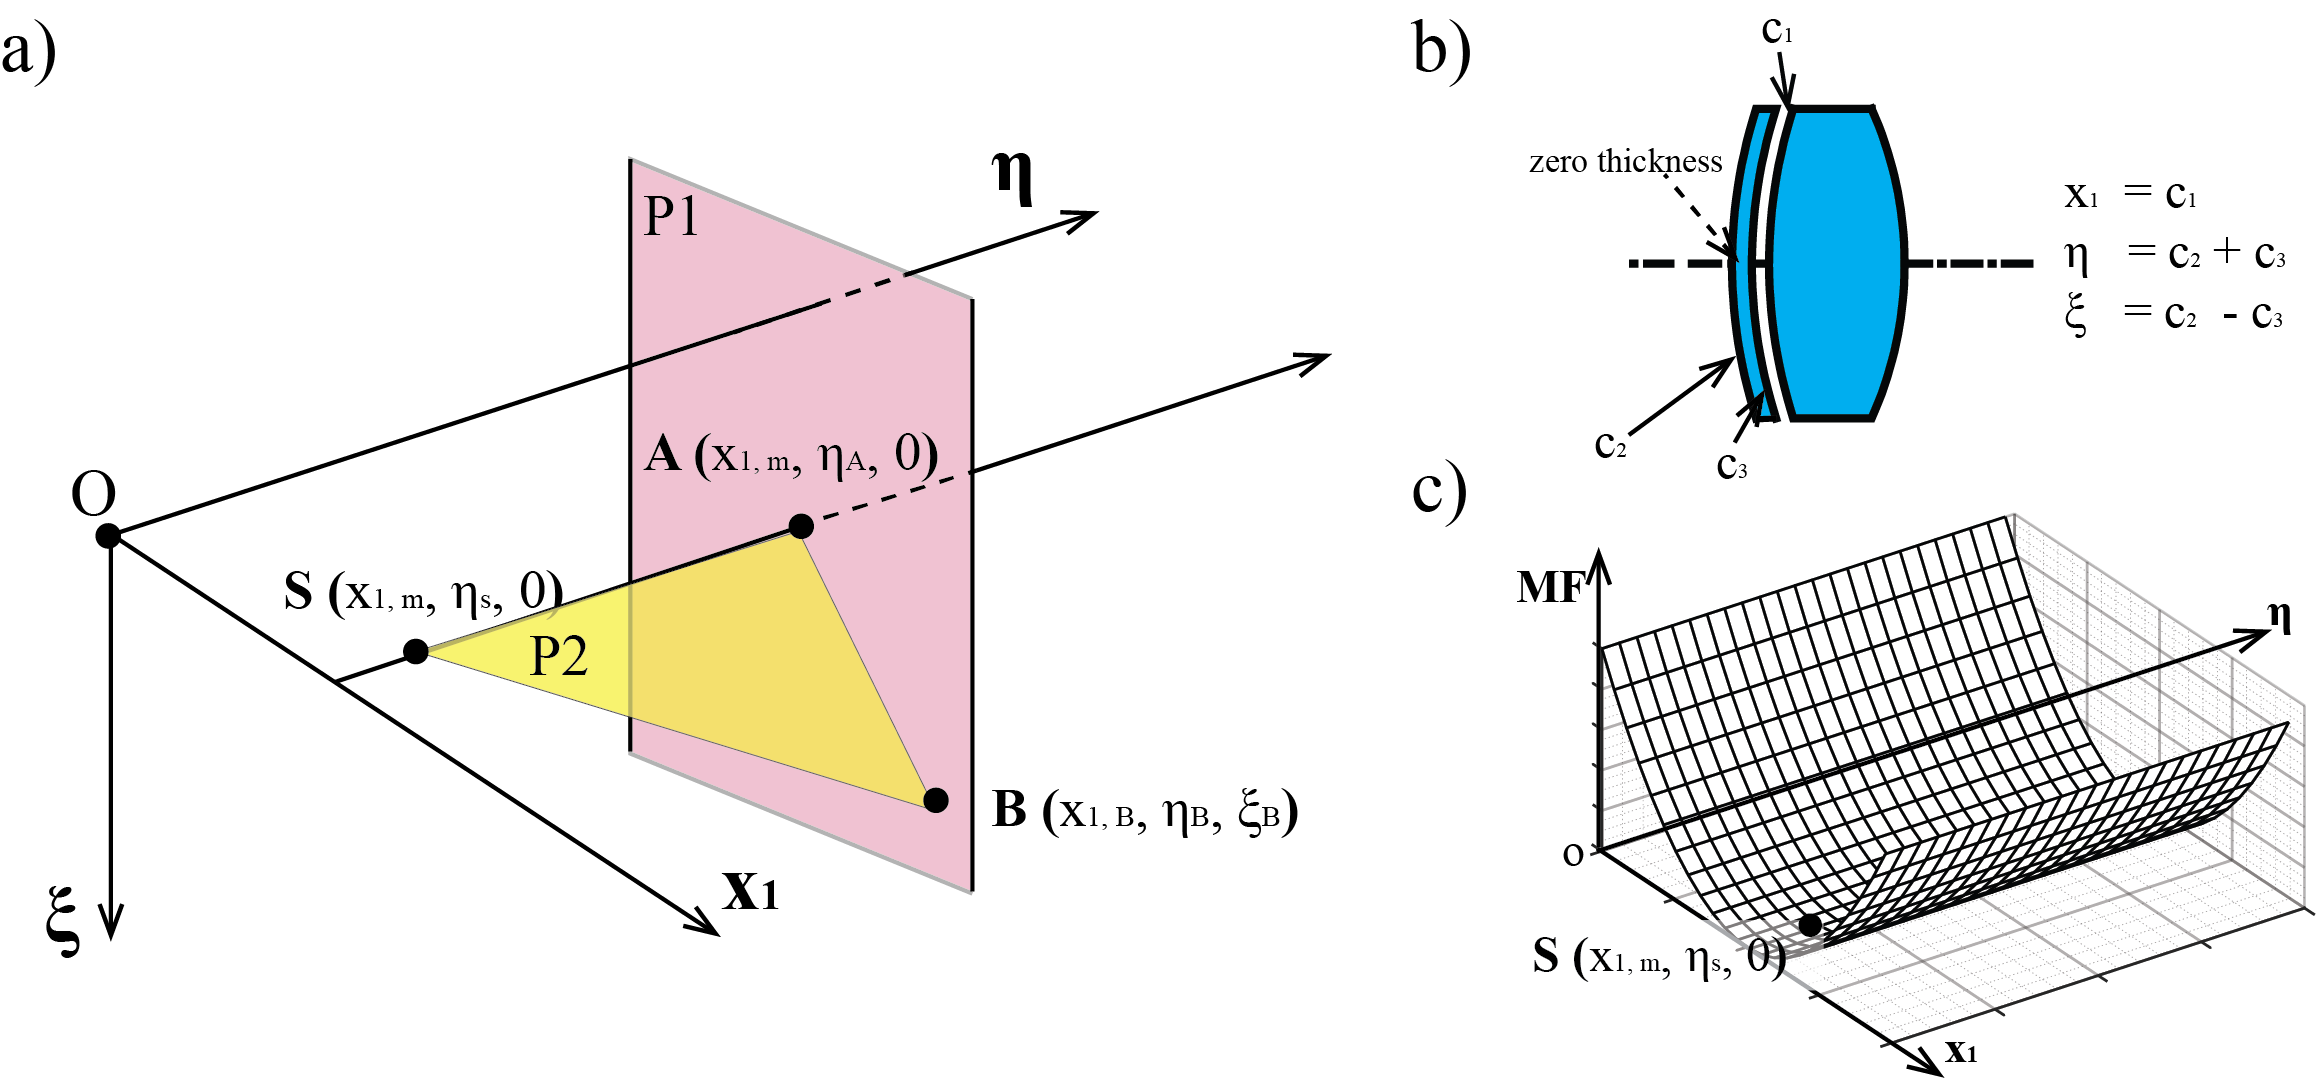
\includegraphics[width=0.985\textwidth]{chapter-4/figures/hyperplane.png}
    \caption{ a) The construction of a 2D plane P2 to visualize the saddle point S in a 3D dimensional example. Point A is a point on the SPC scan line. P1 is a hyperplane perpendicular to line SA. Point B is where the merit function value is minimized on P1. b) Explanation about variables and coordinates. When $\xi = 0$, the $x_1, \eta$ plane includes all the null element systems. c) Example of a merit function landscape in the $x_1, \eta$  plane. $x_{1, m}$ indicates the original minimum values before insertion of the null element.}
    \label{fig:hyperplane}
\end{figure}
In Figure \ref{fig:WAL_demo_sp}(d), the plots along the X and the Y direction show that the value of the merit function is increasing in one direction and decreasing in the other direction. Optimization routes following the descending directions on both sides of the saddle (on the Y-axis shown in Figure \ref{fig:WAL_demo_sp}(d)) lead to two distinct local minima.

\subsubsection{Choices of Starting Point of Local Optimization near the Saddle Point}
Visualizing a saddle point in the 2D plane $P2$ is good for demonstration and helps to choose the optimization direction, however, in practice, it is computationally expensive to look for the 2D plane for each saddle point. As mentioned previously, a common practice is to change the system along the SPC scan line, which means changing the curvatures of the inserted null-element with a small positive and negative value (this value is chosen empirically). The modified systems are the starting points for optimization. The optimization includes two curvature variables in addition to the variables where the minimum (without the null element) is obtained. In the experiment, choosing different values for the curvature change may lead to different minima. This is demonstrated in Figure \ref{fig: scanning_line}, where different values were chosen for the null-element curvature as a starting point to find  the corresponding local minimum. In order to better illustrate the phenomenon, the scan range chosen here (from -0.2 to 0.2) was larger than the curvature changes normally used in practice. From Figure \ref{fig: scanning_line}, it is observed that four different minima were obtained with different values chosen as the starting curvature. The corresponding system shapes and merit function values are shown in Table \ref{table: scanline}. 
\begin{table}[h!]
    \centering
    \captionsetup{justification=centering}
    \caption{Result of the optimization along the scan line (dashed boxes mark the zero-thickness elements).}
    \label{table: scanline}
    \vspace{-1em}
    \hspace*{-16.5pt} %adjusting the position of the plot(table)
    \begin{tabular}{l}
    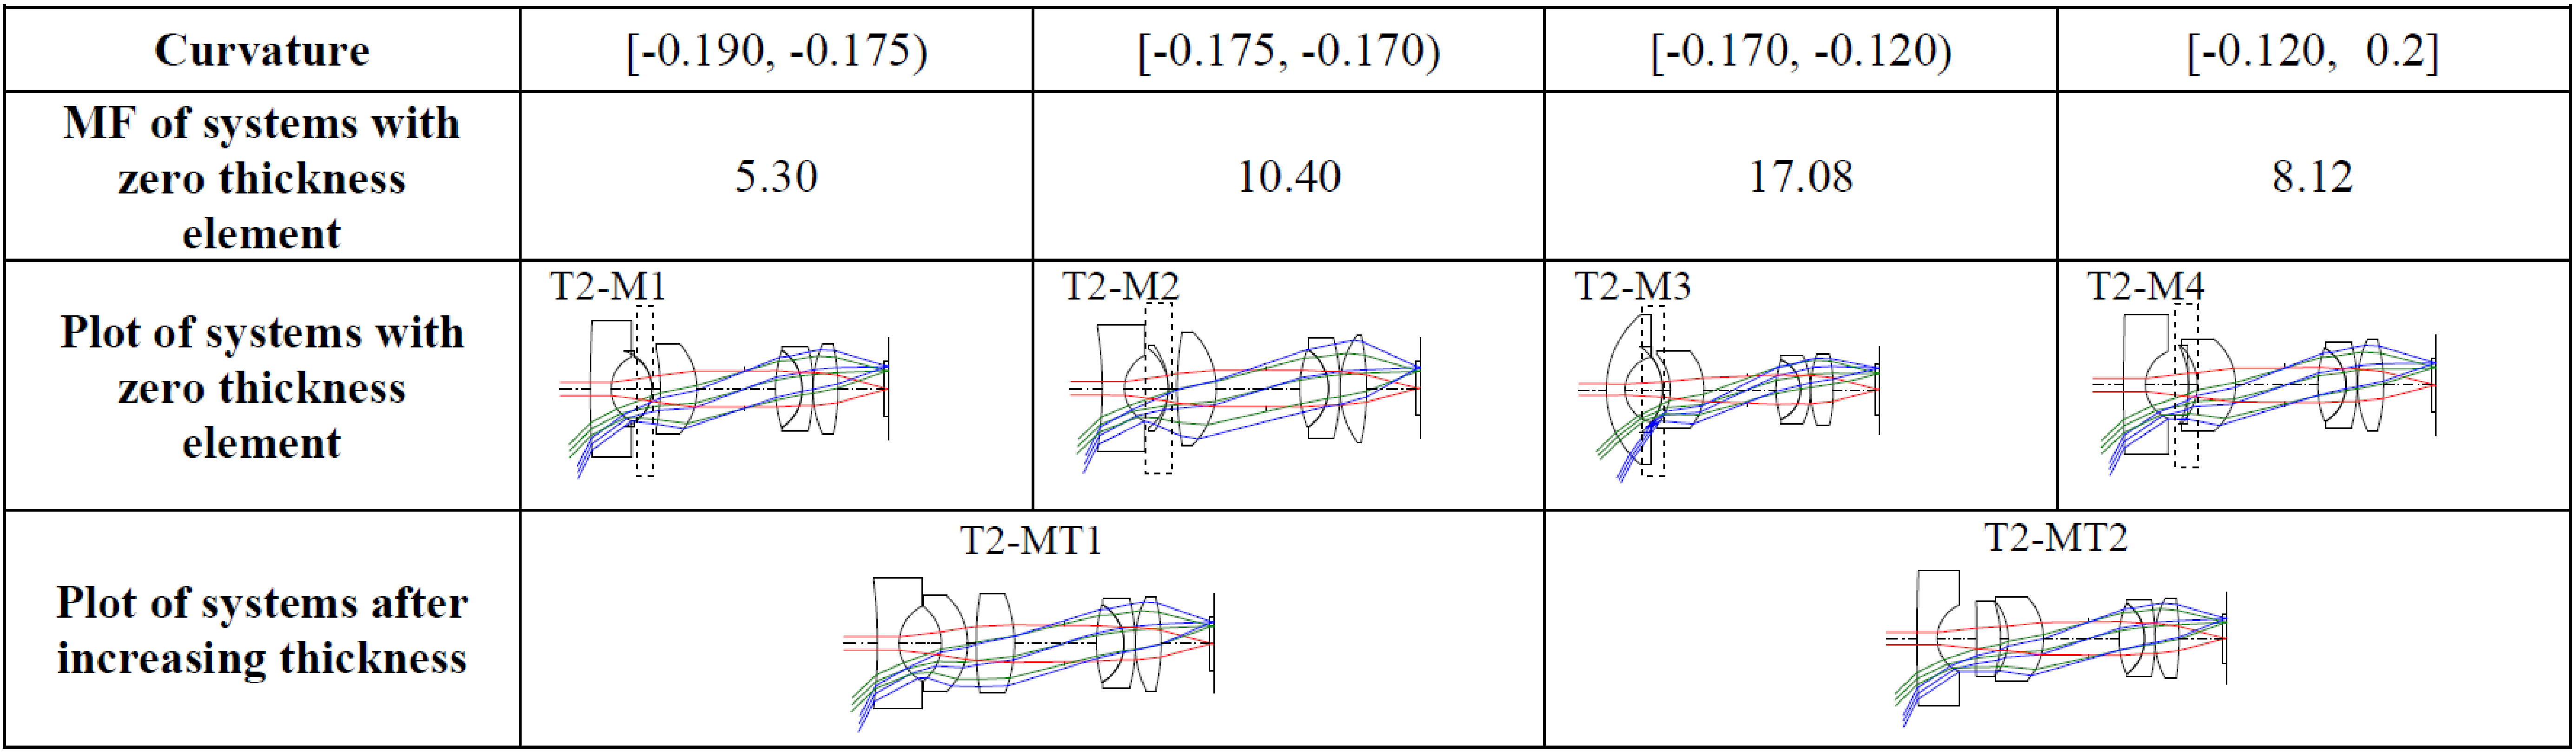
\includegraphics[width=0.98\textwidth]{chapter-4/figures/Line_Opt_table.png}
    \end{tabular}
\end{table}
\begin{figure}[h!]
    \centering
    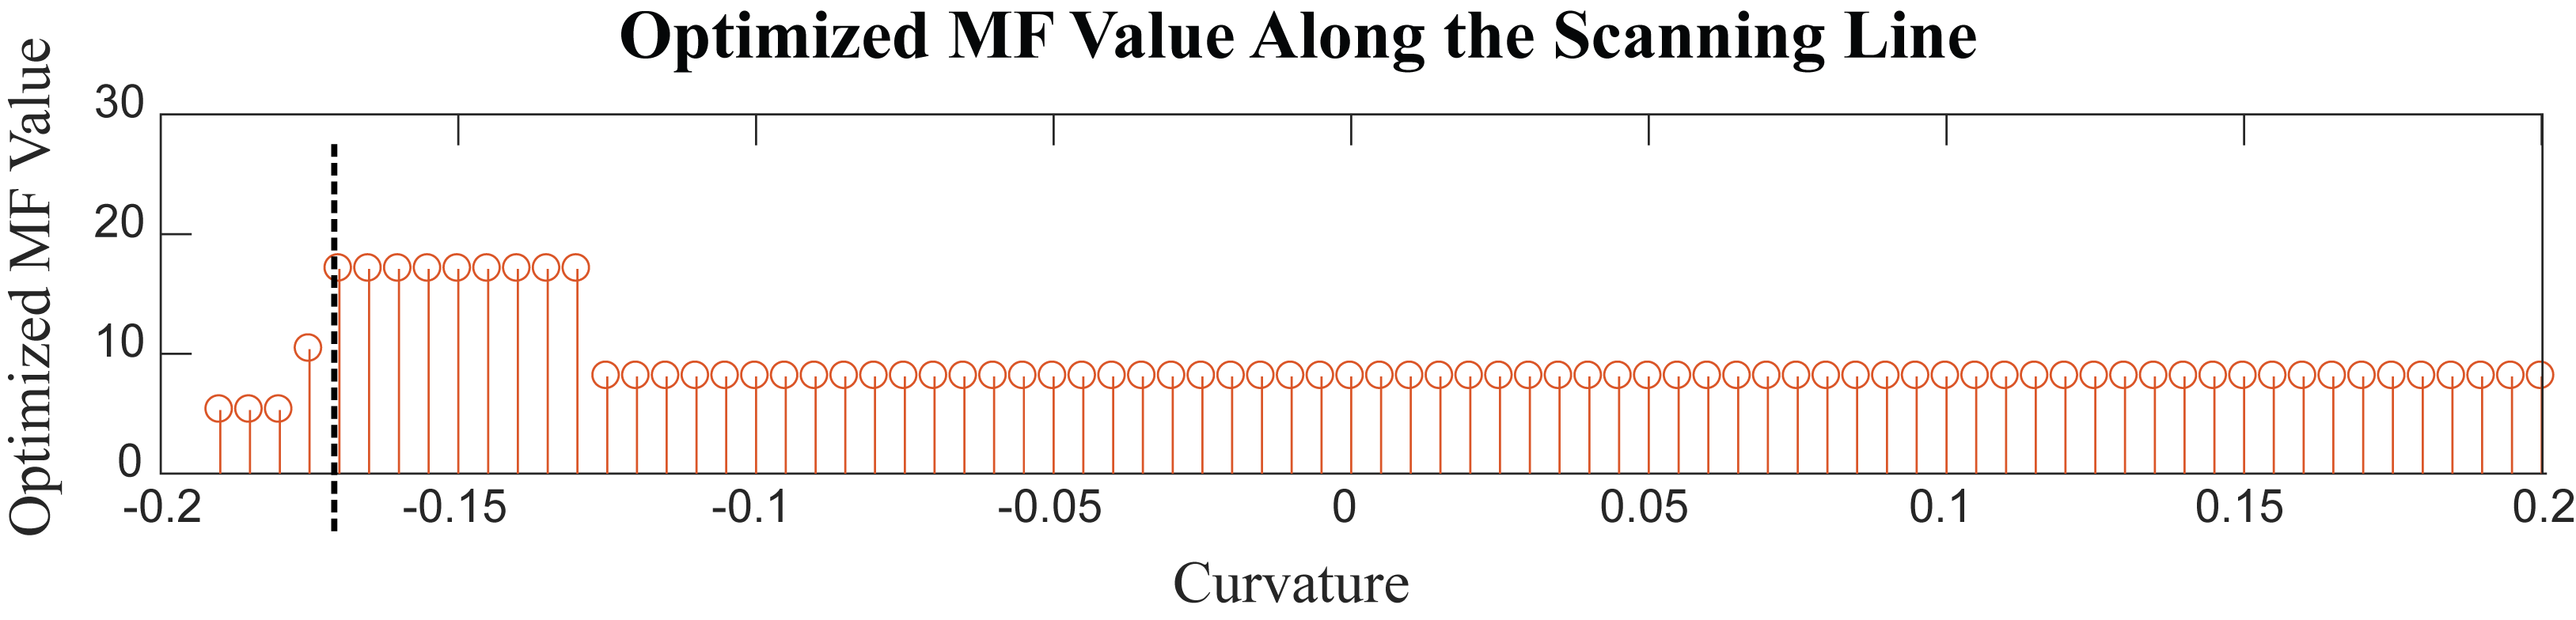
\includegraphics[width=0.95\textwidth]{chapter-4/figures/Scanning_Line_plot.png}
    \caption{Optimized MF value along the scan line. The vertical dashed line indicates the saddle point curvature. The stepsize is 0.05.}
    \label{fig: scanning_line}
\end{figure}

In Figure \ref{fig: scanning_line}, with a curvature step size of 0.05, we see that different local minima are obtained around the curvature value of the saddle point. It indicates that near the saddle point, the local optimization is still sensitive to the choice of the starting point. To better understand the basin of attractions near the saddle point, we have also investigated the cases where the starting point is selected on a 2D plane instead of the one-dimensional scanning line. The constructed saddle point is located in this 2D plane. We have used two different approaches to determine such 2D planes. The first method is to find the plane defined by Equation \ref{eq:u1} and \ref{eq:u2}. On this plane, the saddle point can be visualized and in principle selecting starting points on the opposite side of the saddle point leads to two different local minima. The second method is to construct a plane directly using the two newly inserted variables (two curvatures of the null element). The first method serves as the reference since it clearly captures the ascending and descending directions around the saddle point. However, computing such a plane needs additional effort. The second method is a computation-wise simple way. By comparing the two, we would like to study if a simple approach is sufficient to obtain reliable starting points around the saddle point. 

As shown in Figure \ref{fig:basins}, the plot of the optimization results can also be called the plot of the basins of attraction. The same colour indicates that all starting points from that region (basin) end in the same local minimum after local optimization. The left side of Figure \ref{fig:basins} shows the basins of attraction in a relatively large region, from which the complexity of the optimization landscape can be observed. On the right side of the plot, the region around the saddle point is shown enlarged. In both plots, the scan line divides the basins into two parts: the green part converging to the minimum with a merit function value of 8.12 (T2-M4 in Table \ref{table: scanline}) and the red part converging to the minimum with a merit function value of 5.30 (T2-M1 in Table \ref{table: scanline}). In both cases, we also observe that if the starting points are chosen on the scan line, the optimization may converge to the minimum with a merit function value of 17.08 (yellow color) or the minimum with a merit function value of 10.40 (navy blue color). The red and green regions represent the two basins on both sides of the saddle point. However, in this case, choosing starting points on the scan line may lead to unwanted local minima. Practically, it is still recommended to choose the starting points on the 2D plane defined by the two inserted variables since constructing the hyperplane needs additional steps of constrained optimization. From the plots in Figure \ref{fig:basins}, it is evident that a better way to choose the starting points is to avoid the scan line, for example, by choosing a point on a line that is perpendicular to the scan line. It is also seen that the starting points should not be too far away from the saddle point. Otherwise, the two basins around the saddle point will be missed. In Figure \ref{fig:basins}(b), the saddle point has coordinates $(-0.1702,-0.1702)$. The closest starting point where the optimization converges to an unwanted minimum is $(-0.1713, -0.1675)$. The distance between this starting point and the SP is $0.0029$, which is $1.7\%$ of the absolute value of the curvature at the saddle point. It indicates in this example that even with a small step, optimization can go to a local minimum which is not expected. Practically, it suggests that more than two starting points around the saddle point are needed such that the minima connected to this saddle point is obtained. 

\begin{figure}[h!]
    \centering
    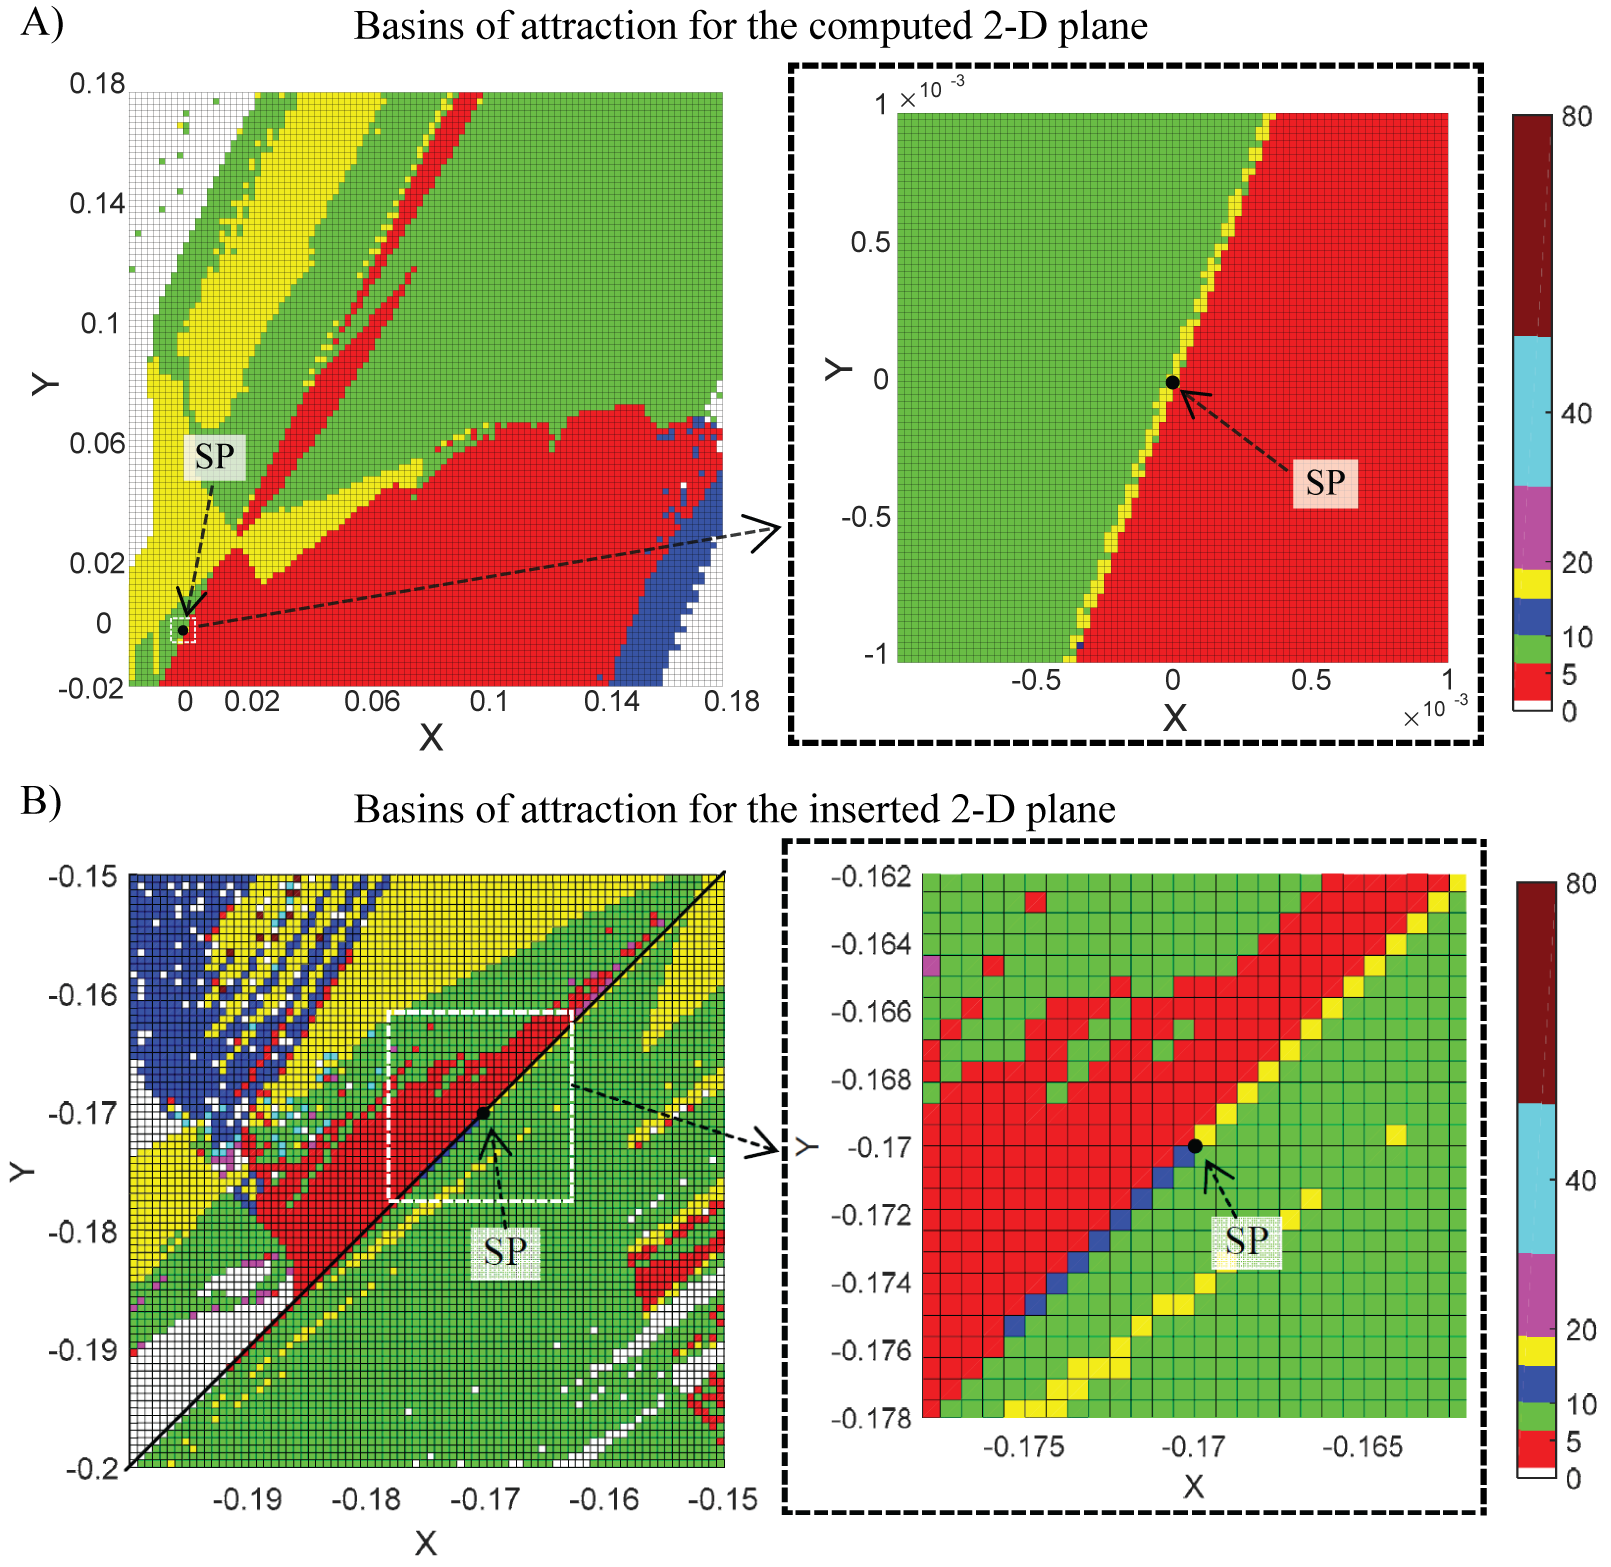
\includegraphics[width=0.8\textwidth]{chapter-4/figures/Basins_two_situations.png}
    \caption{Basins of attraction around the saddle point in 2D planes. a) Computed 2D plane where x and y are the variables defined by equation \ref{eq:u1} and \ref{eq:u2}; b) 2D plane given by the two newly inserted variables. The saddle points (SP) are marked by black dots.}
    \label{fig:basins}
\end{figure}

It is not clear in the presented example why on the scan line the optimization might lead to other solutions than the expected ones. It has been demonstrated in previous research done by van Turnhout \cite{vanTurnhoutThesis2009} (Page 81)\cite{vanTurnhout2009_landscape_instab} that when the damping factor of the damped least square algorithm is sufficiently large, there will be less artefacts shown in the plot of the basins of attraction. A hypothesis is that on the scan line there will also be no artefact locations that cause convergence to a different local minimum. In the example presented here, there is no control over the damping factor because the local optimizer of CODE V is used, hence, it is not possible to identify the cause of the behaviour along the scan line. 

It follows that by using a different position for the extraction of a lens and subsequently applying SPC, it is found in Figure \ref{fig:basins_WAL_M3_S5} that a different behaviour occurs along the scan line. In this case, the third lens element was extracted. As shown in Figure \ref{fig:basins_WAL_M3_S5}, along the scan line there are no starting points that lead to different local minima other than the expected two. Local optimization will either converge into a local minimum in the green region with merit function value MF = 44.53, or to a local minimum in the orange region with MF = 37.82. The white region (MF = 0) indicates ray failure. The furthest starting point with respect to the saddle point, at which the system can still be ray-traced, is at $(-0.1893, -0.1960)$. The coordinates of the saddle point are $(-0.1903, -0.1903)$. The distance between the saddle point and this starting point is $0.0058$, which is $3.0\%$ of the absolute value of the curvature of the saddle point. This is a small distance. It again indicates in this example that optimization can become unstable if the starting points around the saddle points are not chosen properly. Similar to the previous example, it suggests that in practice, more starting points around the saddle points should be selected. 
\begin{figure}[h!]
    \centering
    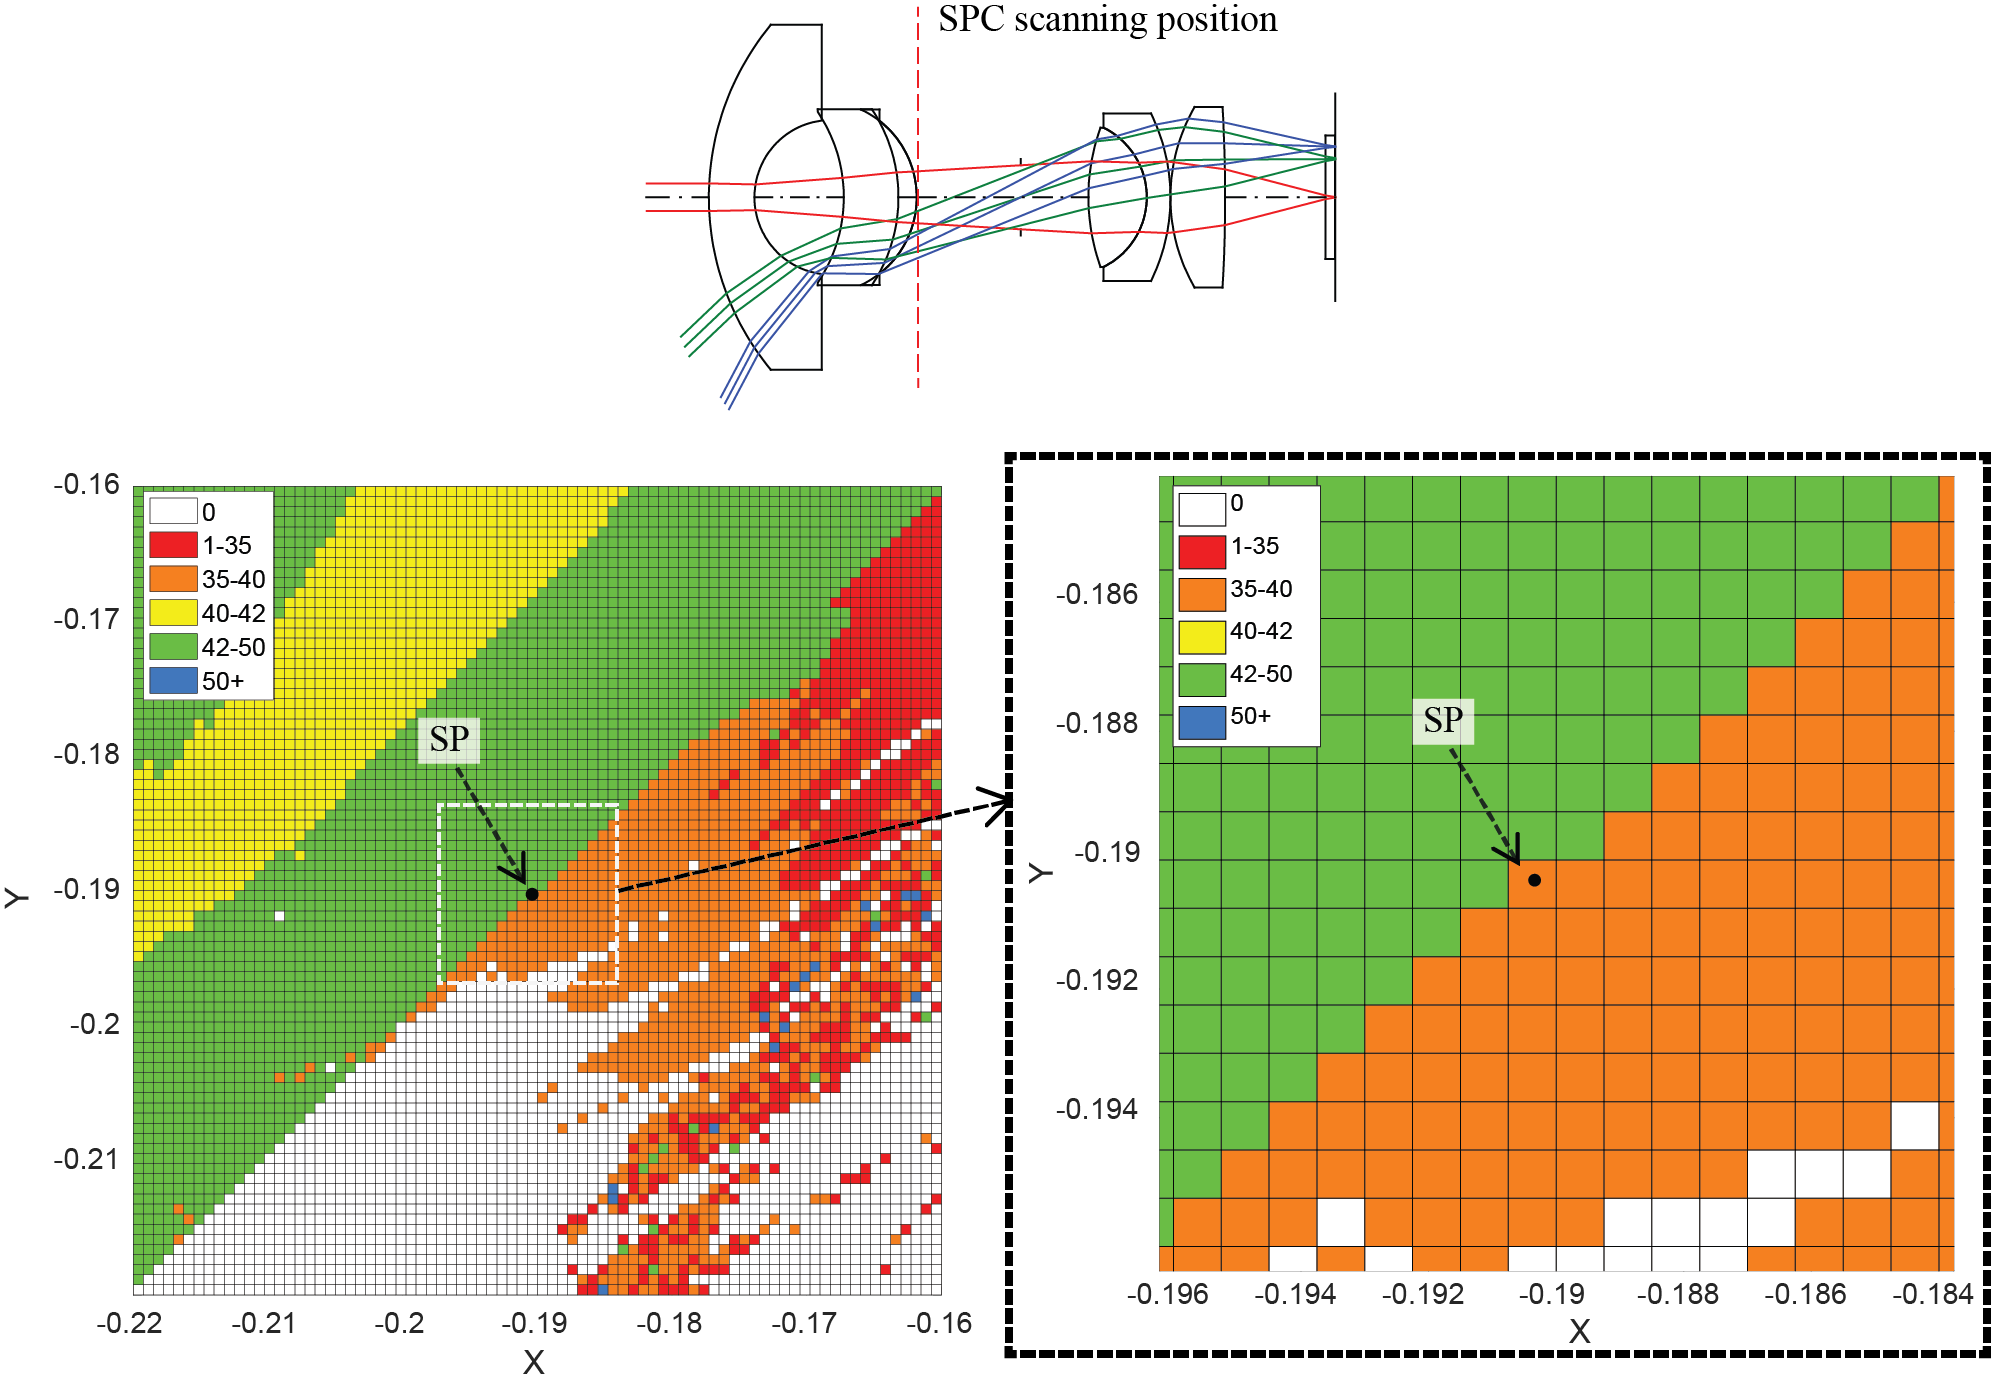
\includegraphics[width=0.8\textwidth]{chapter-4/figures/M3-S5_basins.png}
    \caption{Basins of attraction on the 2D plane defined by the inserted variables at a different scanning position compared to Figure \ref{fig:basins}. Along the scan line (diagonal line in the plot) around the saddle point, there are no starting points for which local optimization leads to minima other than the two next to the saddle point.}
    \label{fig:basins_WAL_M3_S5}
\end{figure}
\subsubsection{Discussion on Local Minima and the Thickness of the Inserted Element}
Until now, the mentioned minima are the minima with zero thickness for the inserted element. To obtain practical solutions, it is necessary to increase the thickness of the zero-thickness element to some nonzero values. In the example of this wide-angle lens, the thickness of the zero-thickness element in each local minimum is restored to the value of the original lens element before extraction. The number of the zero-thickness local minima and the number of local minima after increasing the thickness, are not the same. In Table \ref{table: scanline}, both the zero-thickness minima and the minima after increasing the thickness are listed. When the thickness is increased, T2-M1 merges with T2-M2, and so do T2-M3 and T2-M4. The final results become T2-MT1 and T2-MT2. T2-MT1 corresponds to M1 in Figure \ref{fig:WAL_network} with a merit function value of 4.20. T2-MT2 corresponds to M3 in Figure \ref{fig:WAL_network} with a merit function value of 8.58. 

Figure \ref{fig:thickness_increase} shows the change of merit function value when the thickness of the inserted element is increased in small steps (0.05 mm). In the left plot, the merit function value of T2-M3 changes drastically around thickness 2 mm. The system plots just before and after the peculiar value of  the thickness point are also illustrated in the same figure. Looking at the first lens element, it is seen that the system became very stressed (large curvature values) just before the thickness increased to 2 mm. Ray failure may occur when the thickness is further increased. In case of ray failure, CODE V adapted certain algorithms to modify the system in order to be able to trace the rays. In this example, the system T2-M3 merges with T2-M4 when the thickness is increased to more than 2 mm. On the right side of Figure \ref{fig:thickness_increase}, the merit function value of T2-M4 changes continuously with increasing thickness. The same phenomenon occurs with the other two systems: system T2-M2 merges with T2-M1 right after increasing the thickness. As previously illustrated in Figure \ref{fig:basins}, T2-M1 and T2-M4 correspond to the two expected local minima. It is worth mentioning that the two expected local minima are the two stable ones as shown in this example.

\subsubsection{Section Summary}
With a step by step analysis of applying SPC in this example, it is seen that, for some cases, choosing starting points on the SPC scan line may lead to unexpected local minima (zero-thickness). This may be caused by the specific landscape around the saddle point or numerical artefacts from the optimization algorithmn. Even though these problems do not always occur, examples suggest that a starting point should be chosen outside the scan line to prevent trapping in unwanted local minima. In the plotted basin of attraction, there are features that make the optimization around the saddle point unstable: optimization can reach to an unexpected local minimum or ray failure region. Therefore, choosing more than two starting points with proper distances to the saddle point is needed. In our experiment, we use four starting points: two are on the scan line and two are perpendicular to the scan line. The used distances to the saddle point curvatures are $2.5\%$ of the absolute value of the saddle point curvature (having a zero curvature is rarely the case in practice). In addition to the local optimization, experimental results also reveal that, in some cases, zero-thickness minima obtained in the intermediate steps of SPC are not stable and disappear after increasing the thickness of the inserted element. For the example given here, the final result (two finite-thickness minima) is less dependent on the precise choice of the starting points chosen after obtaining the saddle point.  

\begin{figure}[h!]
    \centering
    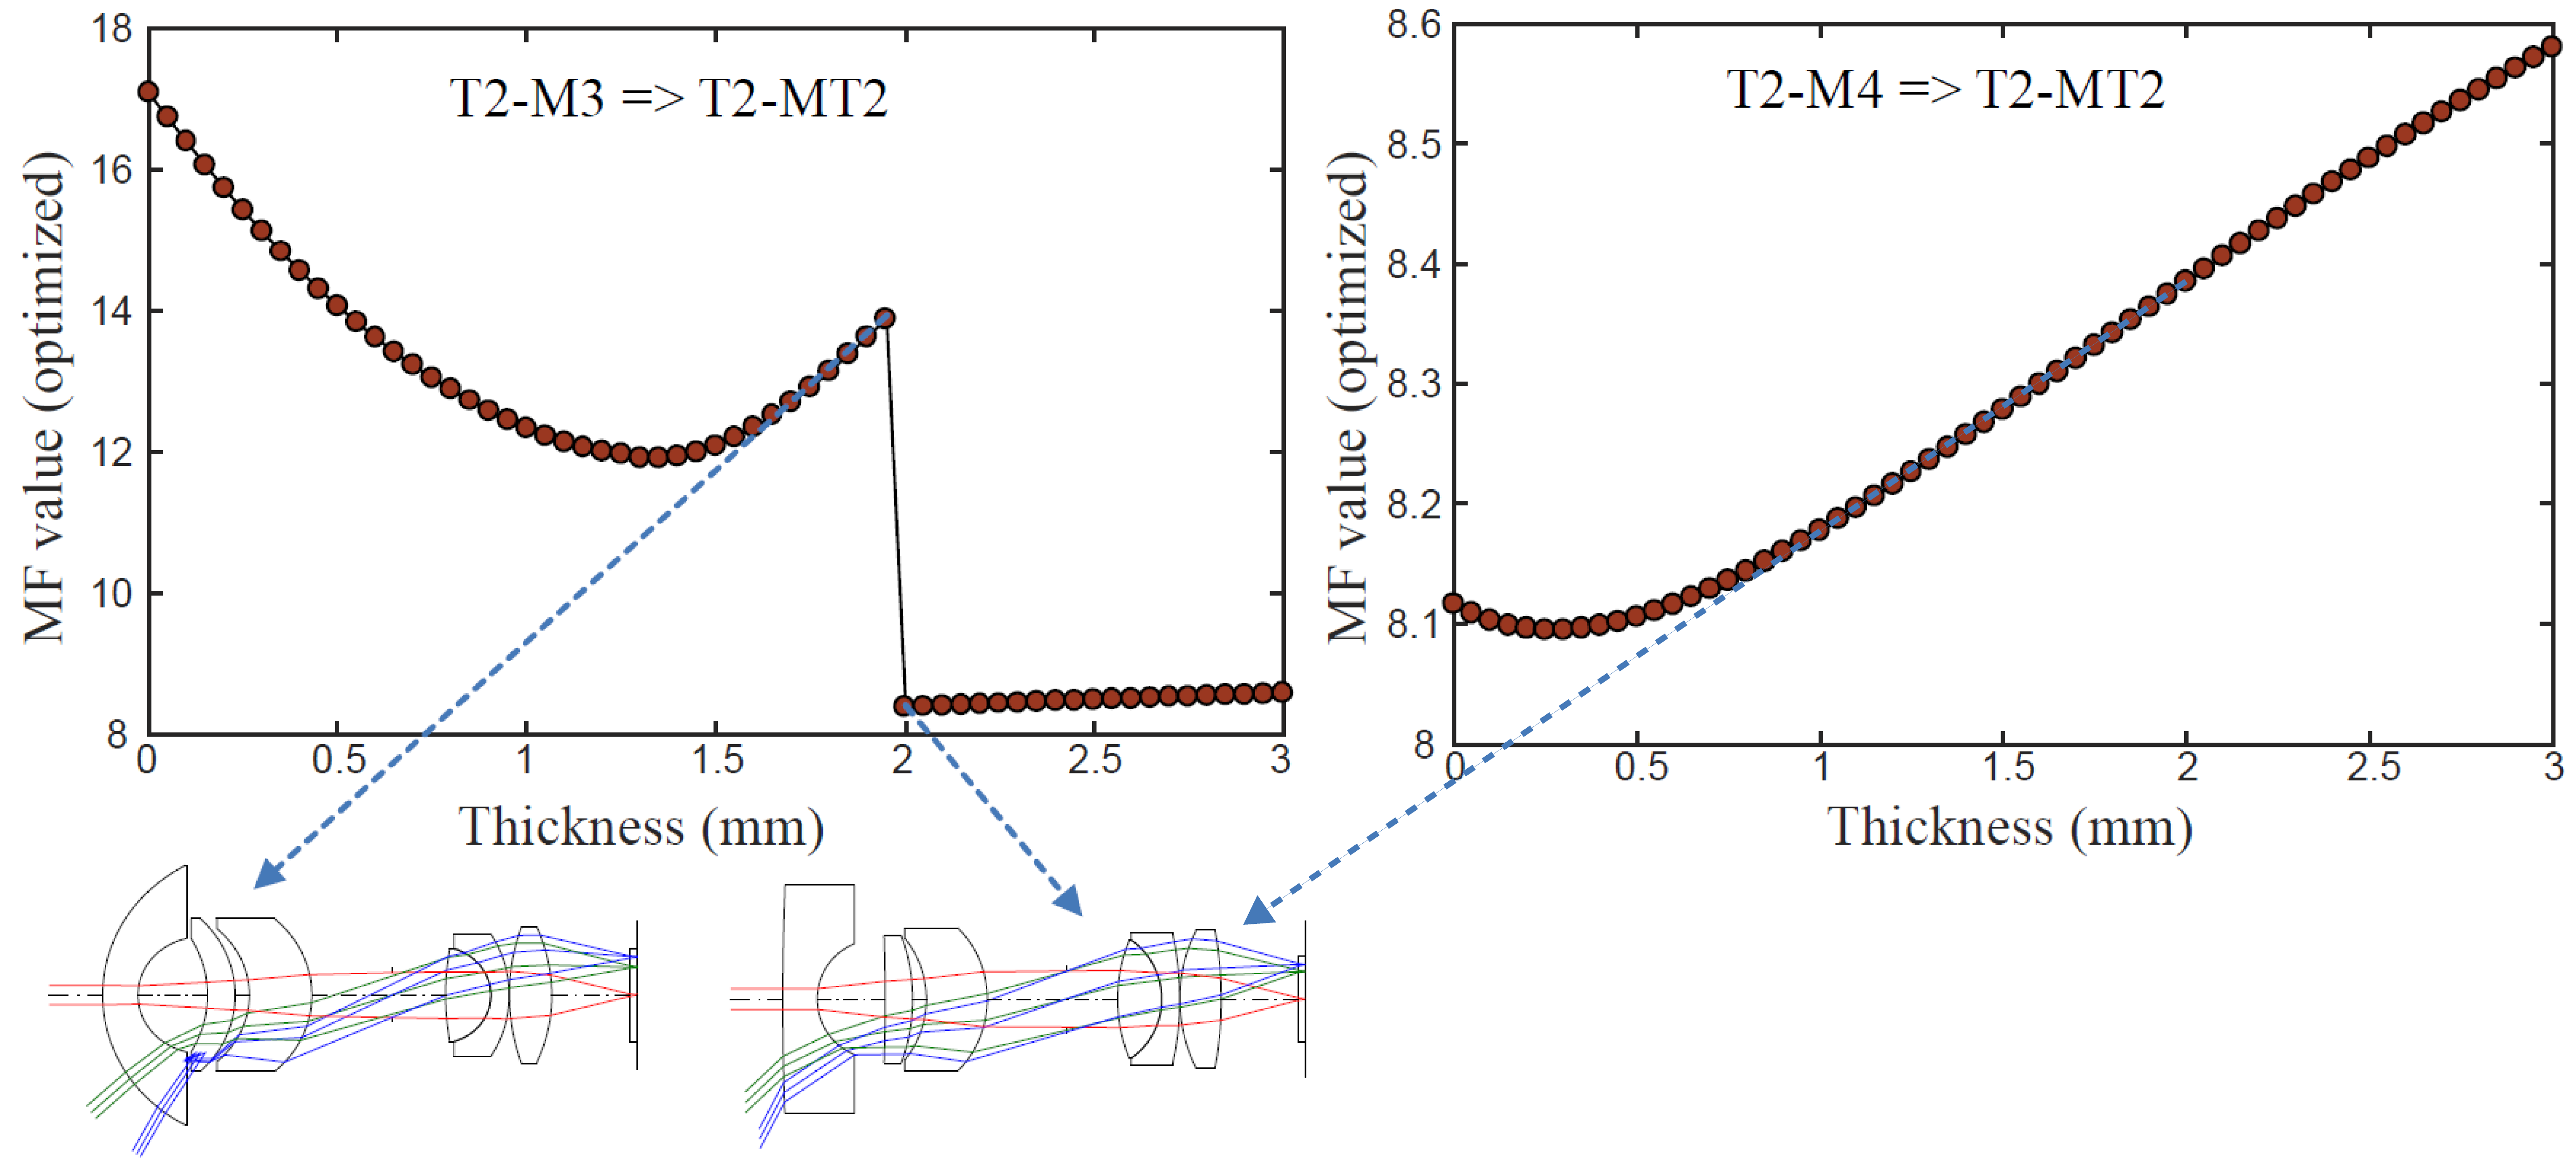
\includegraphics[width=0.8\textwidth]{chapter-4/figures/thickness_increase.png}
    \caption{Change of the optimized value of the merit function while increasing the thickness of the zero-thickness element. T2-M3 and T2-M4 correspond to systems when the thickness is zero. T2-MT2 corresponds to the system when the thickness equals 3 mm. The discontinuity of the left plot indicates the instability due to ray failure around a minimum in the design space. Systems like the left one are usually poor local minima.}
    \label{fig:thickness_increase}
\end{figure}

\section{Combining Designers' Knowledge and SPC to Improve Design Efficiency}
In lens design practice, it is common that multiple design techniques are applied to effectively obtain an optimal solution. The technique can be using a cemented doublet to reduce chromatic aberration, controlling the exit marginal ray angle to keep EFL constant, using a certain optimization method to find better local minima, etc. The SPC method provides a systematic approach to rapidly obtain local minima. However, it does not tell you where the SPC should be applied in an optical system. A straightforward way is to apply many SPCs in a system to generate all the possible local minima. However, this is not always preferred because at a certain phase of the design process, the designer does not really expect a drastic change of the system. In this section, we explore the option of combining designer knowledge and SPC. A UV dry microscope objective is used to show what can be achieved with this approach. 
%I have somehow an established system, where no big change is preferred to be made.  Only local/small adjustment is wanted in order to gain performance improvement. The "localness" depends on each design scenario. The knowledge of the designer is rather "converged" at that point, and deviation from the current system drastically would distract the designer from the current "flow" of thought. On the level of user experience, the global optimizer is not preferred at such a fine and delicate phase of the designing. It might be a good tool at the very beginning to provide ideas for the starting point of the whole design process. 
% In this sense, the SPC shows its advantage since it could help the designer at different stage of the design. It could be used as a tool to navigate a local region of the current design snapshot. The designer can keep her/his sense of control as well as getting acceptable deviations of the design. 

\subsection{Ultraviolet (UV) Microscope Dry Objective}
As a method to search for alternative solutions in lens design, SPC can be automated. In such a scenario, SPC could be used as a global search tool, where, after setting up all the specifications, the program would generate potential solutions for further selection. However, one of the challenges in using SPC, is to choose the proper position for inserting the null element. Conventional design approaches encounter a similar dilemma, namely: when a design process gets stagnated, how to modify the system (adding, extracting or changing) to improve the system? Optical designers usually use their unique insight and experience based on monitoring the aberration, ray properties etc. to make decisions on how to change the system. These approaches and methods used can be very different from person to person, therefore, setting up an algorithm to try out all promising looking options is difficult. If the optical system is relatively simple, it is possible to combine the SPC with approaches based on the designer's knowledge. To use SPC, the modification of the system should be adding or replacing lens elements in the existing system. We will give two examples of how to combine SPC with conventional approaches. 

An ultra-violet (UV) microscope objective is chosen as a starting configuration. The microscope objective is taken from an existing patent\cite{patentvollrath} where its specification is reported. The variation designed for wavelength 325 nm is selected from the patent and reproduced in CODE V. The system consists of seven lens elements. The material used in CODE V is fused silica (LithosilQ from SCHOTT) with a refractive index of 1.4816 at 325 nm. The specification and performance of the system are listed in Table \ref{table: vollrathspec}. With a barrel lens having a focal length of 250 mm, the magnification of the composite microscope becomes 100. The seven lens elements of the system can be divided into three function groups according to a categorization method proposed by Zhang and Gross \cite{ZhangMicroscope2017}: the first lens on the left forms the rear group; the second and third lenses form the middle group, and the rest of the lens elements form the front group. The objective is shown in Figure \ref{fig: vollrathoriginal}. The front group is defined as the one facing to the object in the application, however, during the design it is convenient to work reversely, hence the front group is on the right side in Figure \ref{fig: vollrathoriginal}. According to the same author, existing microscopes can be categorized into three types depending on the functions performed by different groups of lenses. The distribution of the spherical aberration in different groups shown in Figure \ref{fig: vollrathoriginal} indicates that the middle and rear group compensate each other to correct the spherical aberration. This correction behaviour belongs to one of the types described in \cite{ZhangMicroscope2017}.

\setlength{\arrayrulewidth}{.5mm}
\setlength{\tabcolsep}{18pt}
\renewcommand{\arraystretch}{1.2}
\begin{table}[h!]
    \centering
    \captionsetup{justification=centering}
    \caption{System specification and performance of the microscope objective}
    \label{table: vollrathspec}
    \vspace{-1em}
    \begin{tabular}{ p{15em}  c }
    \hline 
    Effective Focal Length (mm) & 2.5\\ 
    Field (real image height, mm) & 0.1\\ 
    Numerical Aperture (NA) & 0.90\\ 
    Operating Wavelength (nm) & 325\\ 
    Working Distance (WD, mm) & 0.6\\ 
    Overall Length (mm) & 25\\
    \midrule
    RMS Wave Front Error (m\textlambda) & 49\\ 
    Strehl Ratio at 0 mm & 0.976\\ 
    Strehl Ratio at 0.1mm & 0.849\\
    \hline
    \end{tabular}
\end{table}

\begin{figure}[h!]
    \centering
    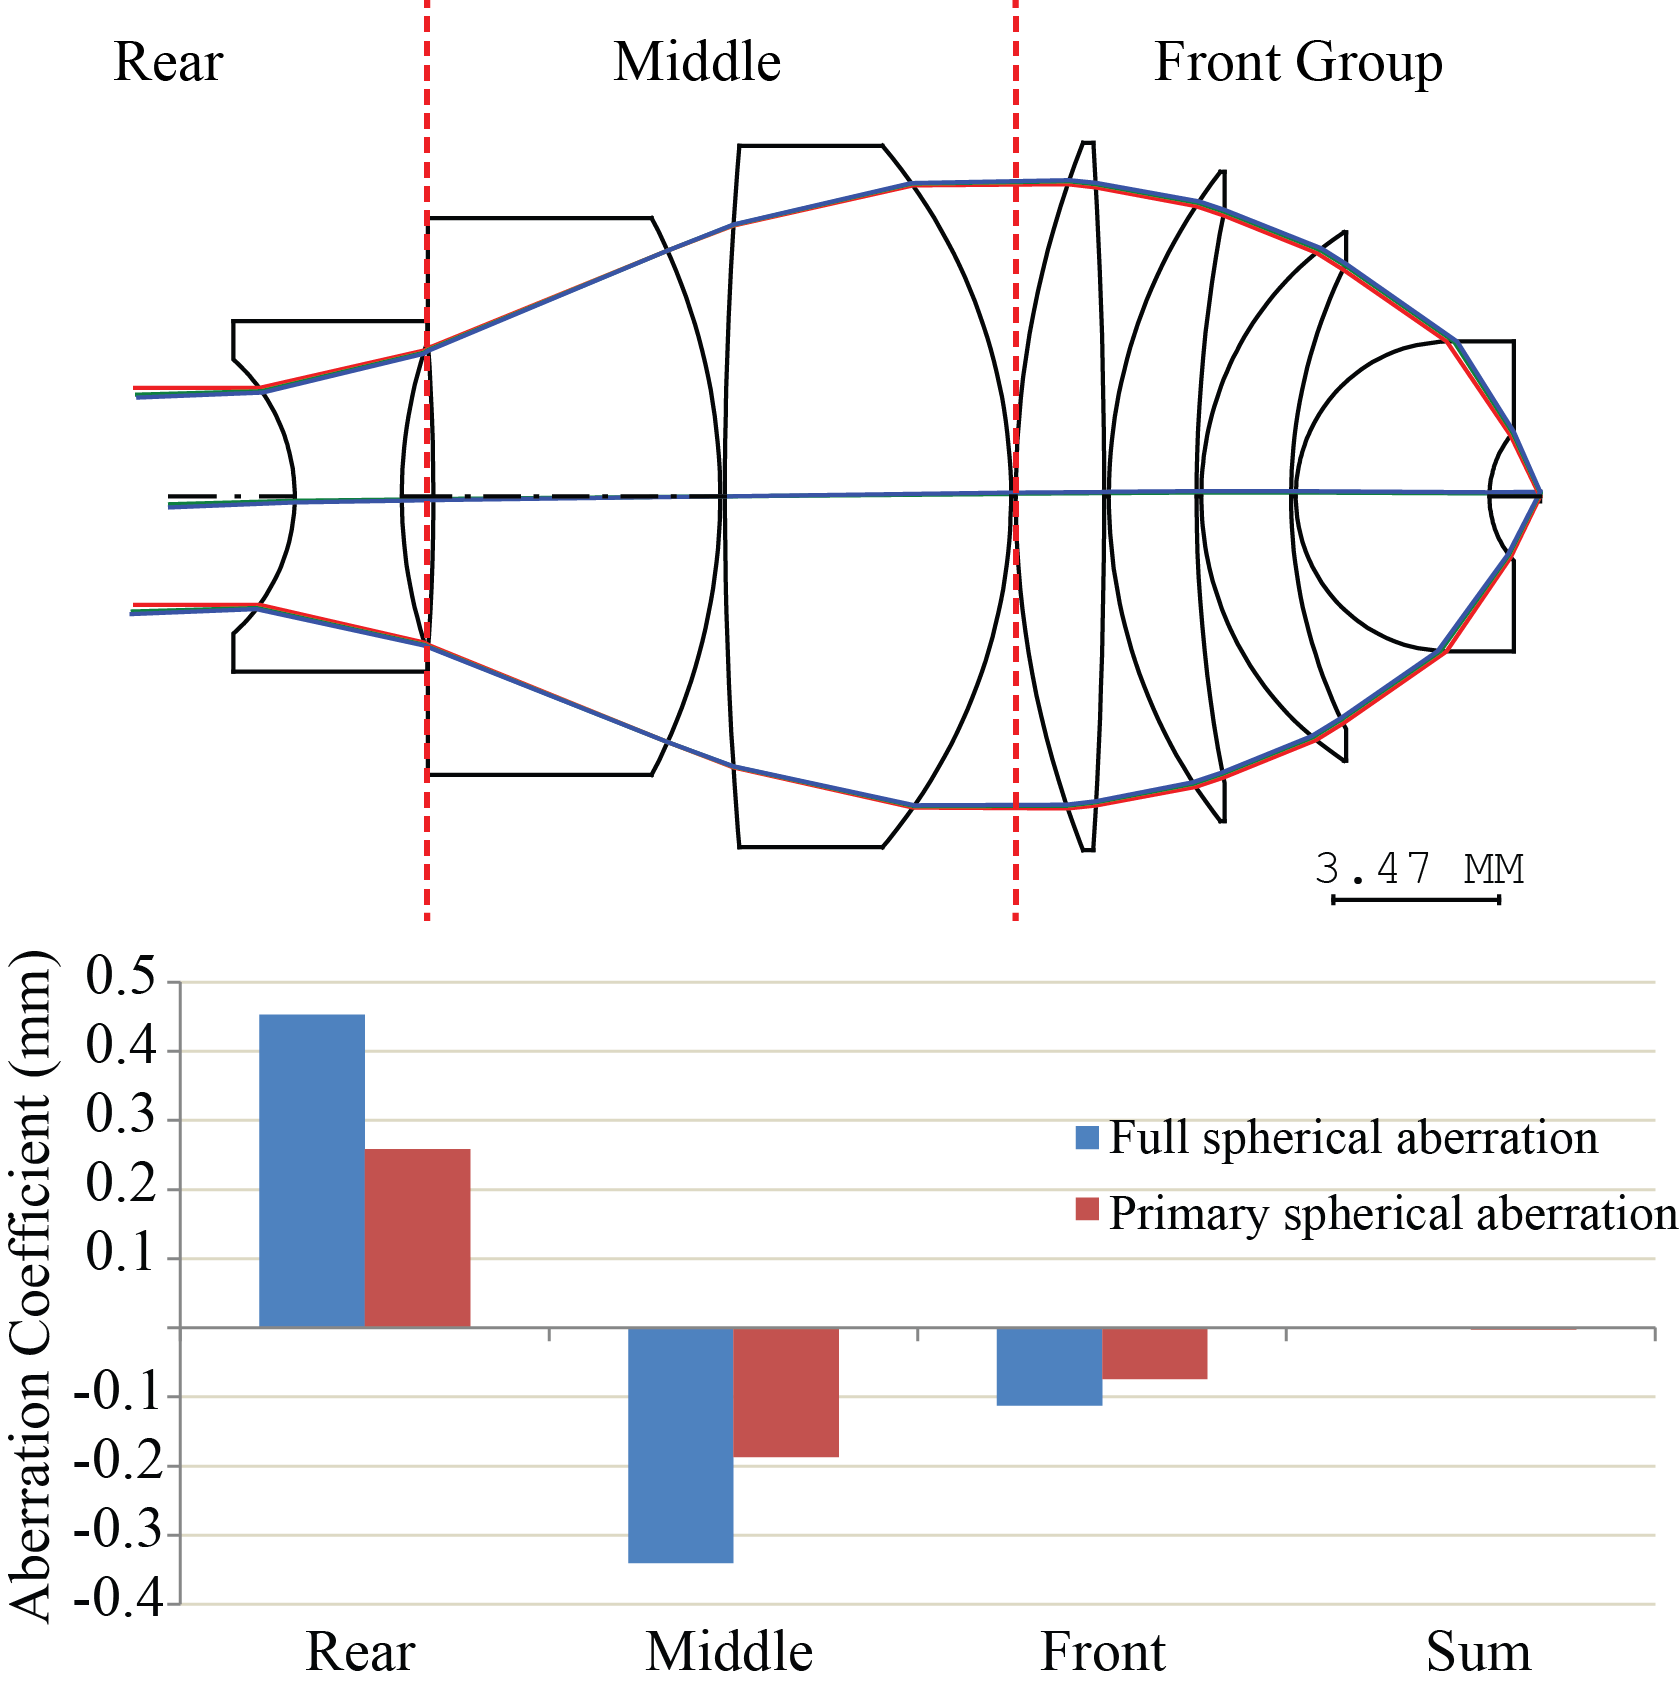
\includegraphics[width=0.55\textwidth]{chapter-4/figures/Vollrath_original.png}
    \caption{System plot of the UV microscope objective \cite{patentvollrath}. The objective can be divided into three groups of lenses. The rear group and middle group compensate each other to correct the spherical aberration \cite{ZhangMicroscope2017}.}
    \label{fig: vollrathoriginal}
\end{figure}

The current system already has a good performance and a compact size, its specifications are listed in Table \ref{table: vollrathspec}. However, if some of the specifications are made more demanding, a certain structural modification of the original system is necessary to keep a satisfactory performance. It is then interesting to investigate how SPC could help to find these modifications. The most simple case to investigate is to add an additional lens element. 

In contrast to a simple design problem, a complex system often needs several constraints to fulfill the design requirements. Before showing the design examples, the handling of constraints in SPC is first discussed in the following section.

\subsection{Constraints in Optical Design Software} \label{Constraints in optical design software}
The wide-angle lens shown in the previous section is a moderately complex system where SPC can be used in a limited number of positions. The system only has one requirement on the specifications that needs to be controlled, namely the EFL. It was controlled by setting the value of the exit angle $\alpha$  of the marginal ray on the last optical surface. Given the EPD and the EFL, the exit marginal ray angle $\alpha$ on the last optical surface can be set in CODE V as:
\setlength{\belowdisplayshortskip}{5pt}
\setlength{\abovedisplayshortskip}{5pt}
\begin{equation} \label{eq:EFLsolve}
\tan\alpha = \frac{EPD}{2\times EFL},
\end{equation}
\noindent Certain design requirements, such as EFL, can be used to force selected parameters to be dependent variables which are solved explicitly to keep the chosen requirements satisfied. In automatic design (optimization), this also makes it possible to reduce the number of independent variables, and thereby save computation effort.

However, in lens design practise, most of the design requirements cannot be explicitly controlled in the  aforementioned way. Constraint function such as equality constraint, inequality constraint, penalty function, etc. are then necessary to be implemented in order to fulfill the various requirements. In lens design software, there are usually different constraint functions for the user to choose so that it is possible to control the system design in different ways. In CODE V for example, there are four different types of constraint functions can be used as shown in Table \ref{table: codevconstraints}.

%table template
%\setlength{\arrayrulewidth}{.5mm}
%\setlength{\tabcolsep}{18pt}
%\renewcommand{\arraystretch}{1.2}
\begin{table}[h!]
    \centering
    \captionsetup{justification=centering}
    \caption{Different types of constraints in CODE V\cite{codevmanual}}
    \label{table: codevconstraints}
    \vspace{-1em}
    \begin{tabular}{ p{0.31\textwidth} | m{0.45\textwidth} }
    \hline 
    \textbf{Constraint Mode} & \textbf{Explanation}\\
    \hline
    Equality constraint (=) & Always active. Handled with Lagrangian Multiplier Method. Constrains exactly to target value of the constraint.  \\
    \hline
    Inequality constraint (>, <) & Only active when the optimization violates the targeted boundary. Handled with Lagrangian Multiplier Method.\\
    \hline
    Weighted function (WTC) & Only used for targeted constraint. Includes a weighted function in the merit function.\\
    \hline
    Penalty function (PTC) & Only used for targeted constraint. Includes a penalty function in the merit function. The penalty function is defined in CODE V with more tuning options than the weight function. It is essentially the same way of constraint implementation as the weight function.\\
    \hline
    \end{tabular}
\end{table}

As seen in Table \ref{table: codevconstraints}, both equality and inequality constraints are handled with the Lagrangian multiplier method. We will show in the following part that these two options treat the constraint by adding new variables to the optimization problem and becomes incompatible with SPC scan requirement. The penalty and weighted function methods treat the constraint by modifying the merit function. 

For SPC, before inserting the null element, it is necessary to optimize the current optical system to a local minimum with a given merit function. However, when the constraint is implemented using the Lagrange Multiplier method, it will not be possible to locate the minimum of the merit function for the given variables. We will explain the reasons for this in the following. 

One of the advantages of using a Lagrange multiplier rule is that it treats  the constraint separately from the merit function, allowing the merit function to be based solely upon image quality-related criteria. For the case of an equality constraint, the optimization of the merit function can be written as follows:
\setlength{\belowdisplayshortskip}{5pt}
\setlength{\abovedisplayshortskip}{5pt}
\begin{equation} \label{eq: MFminCon}
\begin{split}
& \text{minimize}\;\; MF(\textbf{x}), \\
& \text{subject to}\;\; g(\textbf{x}) = 0,
\end{split}
\end{equation}
\noindent where $\textbf{x} = (x_1, x_2, ..., x_N)$ is a vector describing a point in the $N$-dimensional variable space. $g(\textbf{x})=0$ is an equality constraint that the variables have to satisfy. Given that both $MF$ and $g$ have continuous first partial derivatives, a new variable $\lambda$ called a Lagrange multiplier is introduced, and the Lagrange function is defined by
\setlength{\belowdisplayshortskip}{5pt}
\setlength{\abovedisplayshortskip}{5pt}
\begin{equation} \label{eq: LagFun}
\mathcal{L}(\textbf{x},\lambda)=MF(\textbf{x})-\lambda\cdot g(\textbf{x}).
\end{equation}A critical point of Equation \ref{eq: LagFun} has zero gradient and satisfies the following equations
\setlength{\belowdisplayshortskip}{5pt}
\setlength{\abovedisplayshortskip}{5pt}
\begin{subequations} 
\begin{align}
& \nabla_\textbf{x}\mathcal{L}(\textbf{x},\lambda)=\nabla_\textbf{x}MF(\textbf{x})-\lambda\nabla_\textbf{x}g(\textbf{x})=0, \label{eq: LagCondition1} \\
& \nabla_\lambda\mathcal{L}(\textbf{x},\lambda)=g(\textbf{x})=0. \label{eq: LagCondition2}
\end{align}
\end{subequations}
From Equation \ref{eq: LagCondition2}, it is seen that once a critical point of $\mathcal{L}(\textbf{x},\lambda)$ is found, the equality constraint is automatically satisfied. Equation \ref{eq: LagCondition1} indicates that the gradient of the merit function can be expressed as a linear combination of the gradient of the constraints at the critical point. The Lagrange multiplier $\lambda$ acts as the coefficients. The Lagrange multiplier rule states that at the critical point, the value of the constrained merit function is either a maximum or minimum. 
%Note: It is equivalent to say that any direction perpendicular to the gradient of the constraint is perpendicular to the gradient of the merit function. 
In this way, the constrained optimization problem in Equation \ref{eq: MFminCon} is converted to an unconstrained optimization problem. The Lagrange multiplier method converts the original $N$-dimensional problem into a $N+1$-dimensional problem by adding one more variable $\lambda$.  At the critical points of $\mathcal{L}(\textbf{x},\lambda)$, $\mathcal{L}(\textbf{x},\lambda)$ equals $MF(\textbf{x})$. Therefore, the smallest value of $\mathcal{L}(\textbf{x},\lambda)$ at the critical point gives the minimum of the constrained merit function. 

Before performing the SPC scan and adding the null element, the system needs to be firstly optimized to a local minimum. In CODE V, when equality or inequality constraints are applied, it means the Lagrange multiplier method is used. We would like now to investigate the possibility of $\nabla_\textbf{x}MF(\textbf{x}) = 0$ at a critical point of $\mathcal{L}(\textbf{x},\lambda)$. According to Equation \ref{eq: LagCondition1}, satisfying $\nabla_\textbf{x}MF(\textbf{x}) = 0$ requires either $\lambda =0 \;\; \text{or} \;\; \nabla_\textbf{x}g(\textbf{x})=0$. The condition $\lambda = 0$ and $\;\; \nabla_\textbf{x}g(\textbf{x})=0$ both indicate that the local minimum of the unconstrained merit function ($MF$) already satisfies the constraint. This situation is not in general valid. Therefore, $\nabla_\textbf{x}MF(\textbf{x}) \ne 0$ is the typical situation for a critical point of $\mathcal{L}(\textbf{x},\lambda)$. It indicates that the unconstrained merit function is not at its local minimum.  

When performing the SPC scan, two additional variables ($c_1$ and $c_2$, curvatures of the null element) are added to the existing system. The scan of the saddle point uses the unconstrained merit function. In this case, the construction of the saddle point is not starting from a local minimum, therefore, the precondition for performing the SPC is not satisfied.    
%We introduce $x_{N+1} = c_1 + c_2$  and $x_{N+2} = c_1 - c_2$. Then we vary $x_{N+1}$ while $x_{N+2}=0$ until we find a value such that $\partial{MF}/\partial{x_{N+1}} = 0$ .  

The inequality constraint mentioned in Table \ref{table: codevconstraints} can not be implemented for an SPC scan either. The constraint becomes active when the optimization violates the boundary, and remains inactive if the optimization is operated within the defined boundary. When the constraint is active, the same situation occurs that the optimized system is not a local minimum of the unconstrained merit function and SPC can not be performed. 

When constraints are implemented using a penalty function or a weighted function method, the preconditions for performing SPC are satisfied. Both approaches add new terms to the merit function with explicit expressions. The altered merit function is used to optimize the system to a local minimum and the same function is used to perform SPC. 

The modified merit function with a weight function term can be written as the following 
\setlength{\belowdisplayshortskip}{5pt}
\setlength{\abovedisplayshortskip}{5pt}
\begin{subequations} 
\begin{align}
& MF_{W}(\textbf{x})=MF(\textbf{x})+\sum_{i=1}^{m}W_i(\textbf{x}), \label{eq: MFWeight} \\
& W(\textbf{x})=(wt\cdot \Delta C)^2. \label{eq: WTC}
\end{align}
\end{subequations}
where the summation indicates that multiple weight functions can be added, $wt$ is the weighting factor set in CODE V, and $\Delta C$ is the departure of the constraints from its target. Using the penalty function replaces the weight function term in Equation \ref{eq: MFWeight} with a penalty function described as the following in CODE V
\setlength{\belowdisplayshortskip}{5pt}
\setlength{\abovedisplayshortskip}{5pt}
\begin{equation} \label{eq: PTC}
P = wt*(\frac{\Delta C}{half \, width})^{\frac{exponent}{2}},
\end{equation}where ${half \, width}$ and $exponent$ are two additional variables for tuning the penalty function. If the ${half \, width}$ is set to $1$ and the $exponent$ is set to $4$, the penalty function in Equation \ref{eq: PTC} is the same as the weight function in Equation \ref{eq: WTC}. The two approaches for implementing the constraints are essentially identical. They both provide a less rigid control compared to the Lagrange multiplier method. The penalty function mode is ideal for the "soft constraints", which are constraints that have an acceptable range of values \cite{codevmanual}. In the next section, where the complex UV microscope objective is investigated, the constraints are implemented with the weighted function.

\subsection{Applying SPC to Induce Structural Changes in Lens}
%add some text to elaborate the title
When trapped in a local minimum, it is useful to introduce structural change in order to obtain different local minima with significant changes in the values of the merit function. The structural change refers to changes such as using a lens with a positive power instead of a negative one, adding a new element into the system, etc. In this section, we focus on two cases where structural changes are needed for the systems to meet a higher requirement. In the first case, the NA of the system is further increased from 0.90 to 0.95. In the second case, the working distance of the system is increased from 0.6 mm to 2.5 mm. We show how SPC can be effectively applied to obtain new local minima. 
%We demonstrate that SPC

\subsubsection{Increasing NA of the Objective}
For a high-resolution microscope objective, high NA is always required. The first example is to increase the NA of the microscope objective from 0.90 to 0.95. The rays can still be traced after the modification, i.e. in the case considered no ray failure occurs after the increase of the NA. The system is then optimized with a wavefront error function. An EFL constraint and a working distance constraint are applied with the equality constraint mode. Figure \ref{fig: vollrathNA90295} shows that the change of the system shape \footnote{A system shape is determined by the bending of each lens element, the thicknesses of the lens elements and  the distance between them.} is mainly in the thickness of the elements. The bending \footnote{The definition of the bending factor is given in Equation \ref{eqn: bending factor}.} of each element remains almost unchanged. From Table \ref{table: NAchange}, it is seen that the performance of the system deteriorates after increasing the NA. A major cause is that the spherical aberration (especially the high-order spherical aberration) increases with increasing NA. In traditional approaches, structural changes to the system would be made by which the number of degrees of freedom increases to be able to reduce the aberration. These kinds of structural change could, for example, be replacing a spherical surface by an asphere, adding extra lens elements, or splitting existing lens elements. In the following examples, the introduced changes are adding or splitting lens elements.

\begin{figure}[h!]
    \centering
    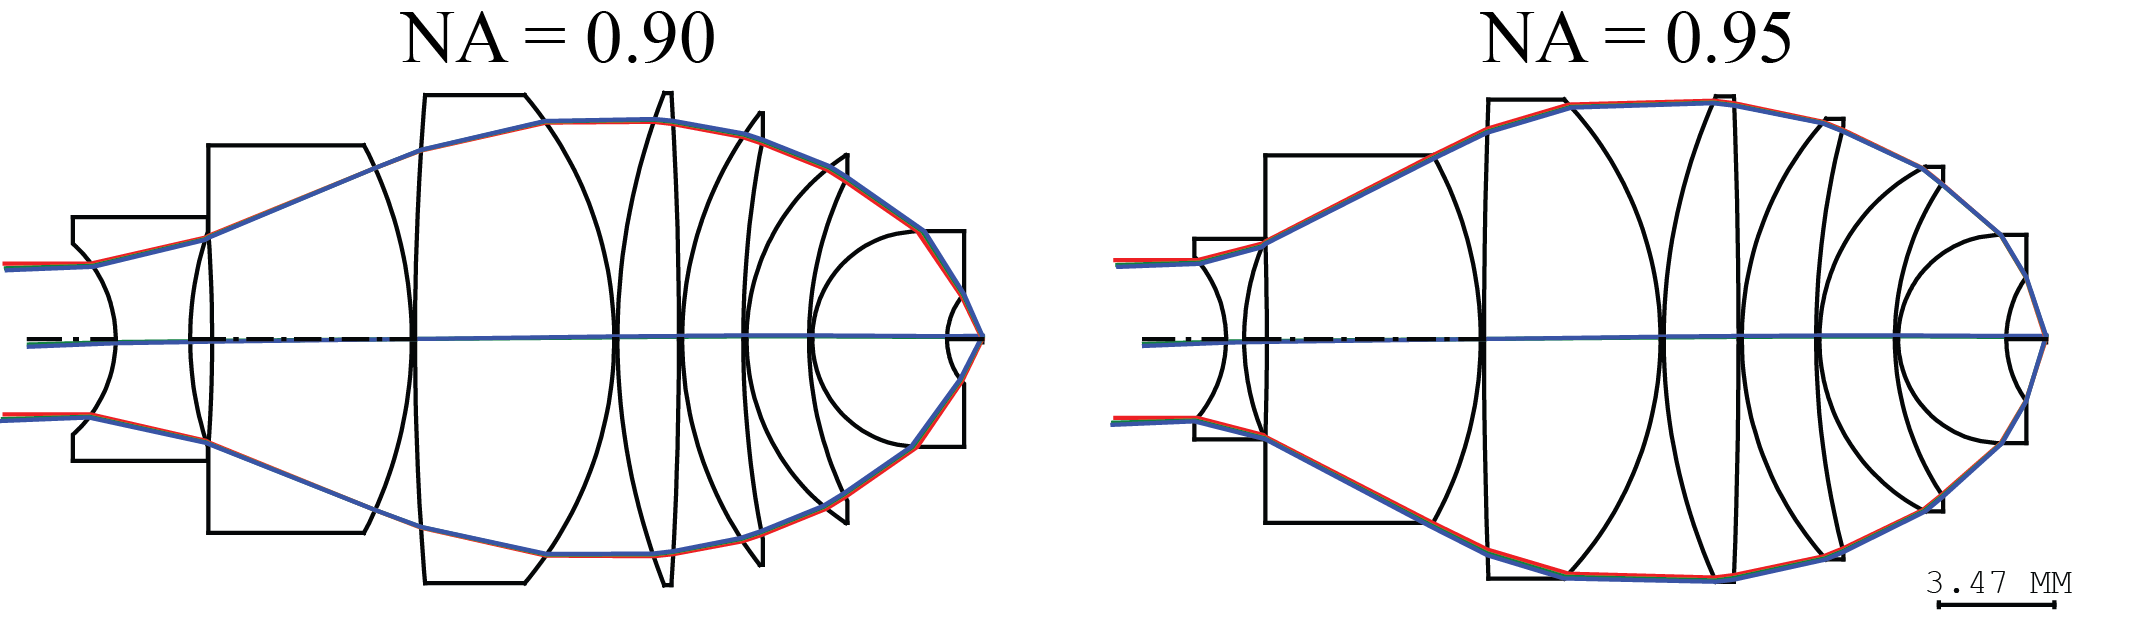
\includegraphics[width=0.6\textwidth]{chapter-4/figures/Vollrath_NA90295.png}
    \caption{Change of the system shape after increasing the NA from 0.90 to 0.95.}
    \label{fig: vollrathNA90295}
\end{figure}

%table template
\setlength{\arrayrulewidth}{.5mm}
\setlength{\tabcolsep}{18pt}
\renewcommand{\arraystretch}{1.2}
\begin{table}[h!]
    \centering
    \captionsetup{justification=centering}
    \caption{Change of the system performance with increasing NA}
    \label{table: NAchange}
    \vspace{-1em}
    \begin{tabular}{ c c c }
    \hline 
     Numerical Aperture & 0.90 & 0.95\\ 
     \cmidrule{2-3}
    RMS Wavefront Error (m\textlambda) & 49 & 111  \\ 
    Strehl Ratio at 0 mm & 0.976 & 0.833\\
    Strehl Ratio at 0.1 mm & 0.849 & 0.386\\
    \hline
    \end{tabular}
\end{table}

With the separation of the system into different function groups, it is possible to understand the function of different parts of the system which provides insight when structural change is needed. It follows from Figure \ref{fig: vollrathoriginal} that the rear and middle group compensate each other to correct the spherical aberration. A reasonable strategy is then to introduce structural changes in these two groups, namely by adding or splitting elements in the rear and the middle group of the system. Based on this insight, four different positions are chosen in the rear and the middle group to add or split elements in the usual way. The resulted system shapes are shown in Figure \ref{fig: vollrathNAtrad}. It is worth pointing out that with the traditional approach of adding or splitting lens, each operation only yields one solution. The performance of the resulting systems are listed in Table \ref{table: vollrathNAtrad}. The data from the table reveal that out of four, one (the number 4 system) has satisfactory performance. For a satisfactory performance, the criteria used here are that the Strehl ratio is above 0.8 for all fields and the wavefront RMS is below $\lambda/14$ \cite{patentvollrath}, for which value the system is considered to be diffraction-limited. In Figure \ref{fig: vollrathNAtrad}, the inserted or split element is highlighted by shading. For operation \circled{1}, the insertion of the lens results in an additional shell lens in the front group. It gives four new degrees of freedoms (two curvatures, one lens thickness, and an air space thickness) for optimization. However, the performance of the optimized system is not satisfactory. Operation \circled{2} splits one of the lens elements in the middle group and thereby distributing its original power to two lens elements. The same happens in the case of operation \circled{3}. Both operations \circled{2} and \circled{3} produce only slightly better results than operation \circled{1}, however, neither of them is good enough. Splitting the lens element in the rear group in operation \circled{4} produces a different system shape compared to the other three and the original system. A reverse-bended element is created (second element from the left), which forms a narrow air gap with the element to the right of it. This kind of air gap is effective for introducing high-order spherical aberrations, which balances the high-order spherical aberrations introduced by other parts of the system \cite{ZhangGross+2019+349+384}. 

\begin{figure}[h!]
    \centering
    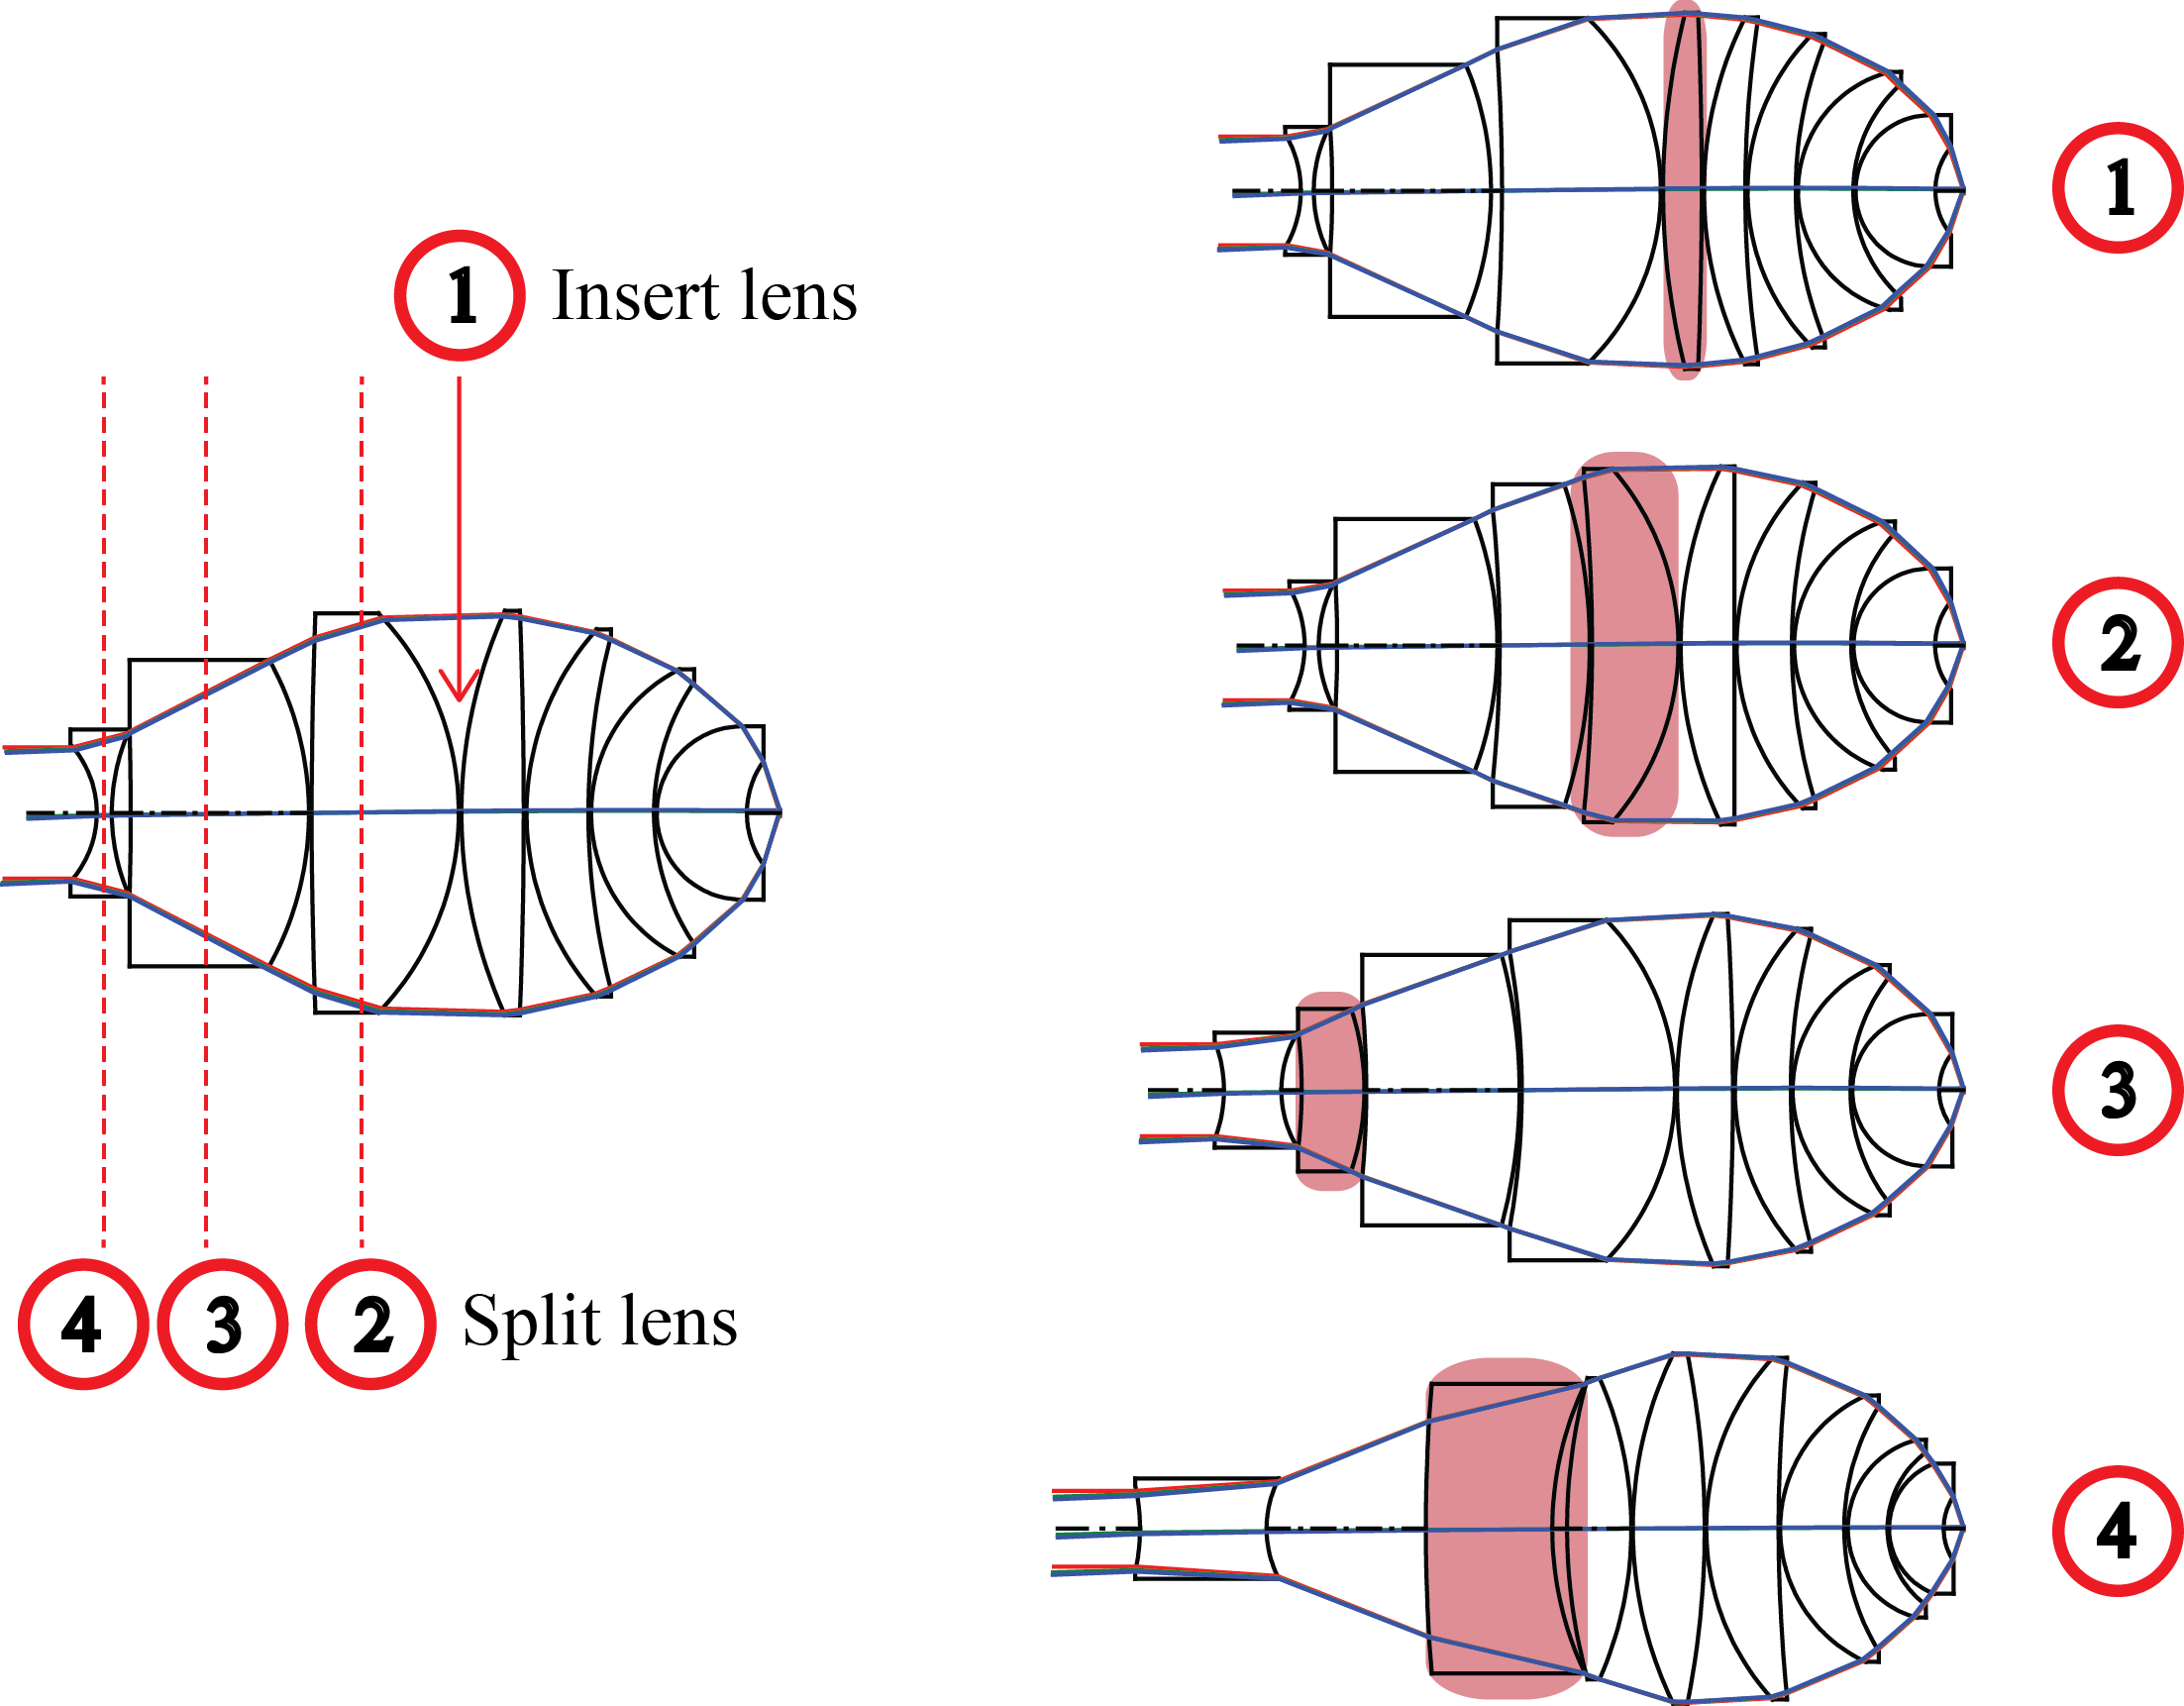
\includegraphics[width=0.7\textwidth]{chapter-4/figures/Vollrath_NATradition.png}
    \caption{Introducing structural change in the traditional way for system performance improvement. Four operations have been executed on the NA 0.95 system resulting in four different results. The inserted or split element is highlighted by shading.}
    \label{fig: vollrathNAtrad}
\end{figure}

\setlength{\arrayrulewidth}{.5mm}
\setlength{\tabcolsep}{18pt}
\renewcommand{\arraystretch}{1.2}
\begin{table}[h!]
    \centering
    \captionsetup{justification=centering}
    \caption{System performance for the systems shown in Figure \ref{fig: vollrathNAtrad}}
    \label{table: vollrathNAtrad}
    \vspace{-1em}
    % \hspace*{-10pt} %adjusting the position of the plot(table) !!!!
    \begin{adjustbox}{max width=\textwidth, center}
    \begin{tabular}{c c c c c}
    \hline 
     No. & \textbf{1} & \textbf{2} & \textbf{3} & \textbf{4}\\ 
     \midrule
    RMS Wavefront Error (m\textlambda) & 119 & 117 & 99 & 41 \\ 
    Strehl Ratio at 0 mm & 0.736 & 0.769 & 0.832 & 0.985\\
    Strehl Ratio at 0.1 mm & 0.428 & 0.453 & 0.548 & 0.882\\
    \hline
    \end{tabular}
    \end{adjustbox}
\end{table}

Based on the insight on where the change should be introduced in the system, SPC scans were performed at four positions in the system. Figure \ref{fig: VollrathSPCcaseNA} presents the results from SPC scans. From four scans, a total number of eighteen solutions were obtained. Besides four solutions which are identical to the ones obtained with the traditional method, fourteen extra solutions were obtained. Their performance is listed in Table \ref{table: vollratSPCcaseNA}. Out of the eighteen solutions, nine reach satisfactory results. Solution \circle{4}A and \circle{4}D even show better performance than the best one obtained by the traditional method (No.4 in Table \ref{table: vollrathNAtrad}). Among all the solutions, \circled{1}A and \circled{2}B have very close system shapes. One is the result from the left bending of the glass lens, and the other is the result of the right bending of the air lens. As explained in Chapter \ref{chapter_SPC_method_reccomendation}, there are two different ways to apply SPC, which lead to the same solution in this case.

\begin{figure}
  \begin{adjustbox}{addcode={
    \begin{minipage}{\width}}{
    \captionsetup{margin=0em}
    \caption{Eighteen solutions from four SPC scans. The dashed line indicates constructing an air lens inside a lens element (equivalent to splitting lens). The solid line indicates constructing a glass element in the air space (equivalent to add lens). In comparison with Figure \ref{fig: vollrathNAtrad}, solution \textcircled{\scriptsize{1}}C, \textcircled{\scriptsize{2}}D, \textcircled{\scriptsize{3}}C, and \textcircled{\scriptsize{4}}D are the ones obtained with conventional approach.}\label{fig: VollrathSPCcaseNA}
    \end{minipage}},rotate=90,center}
    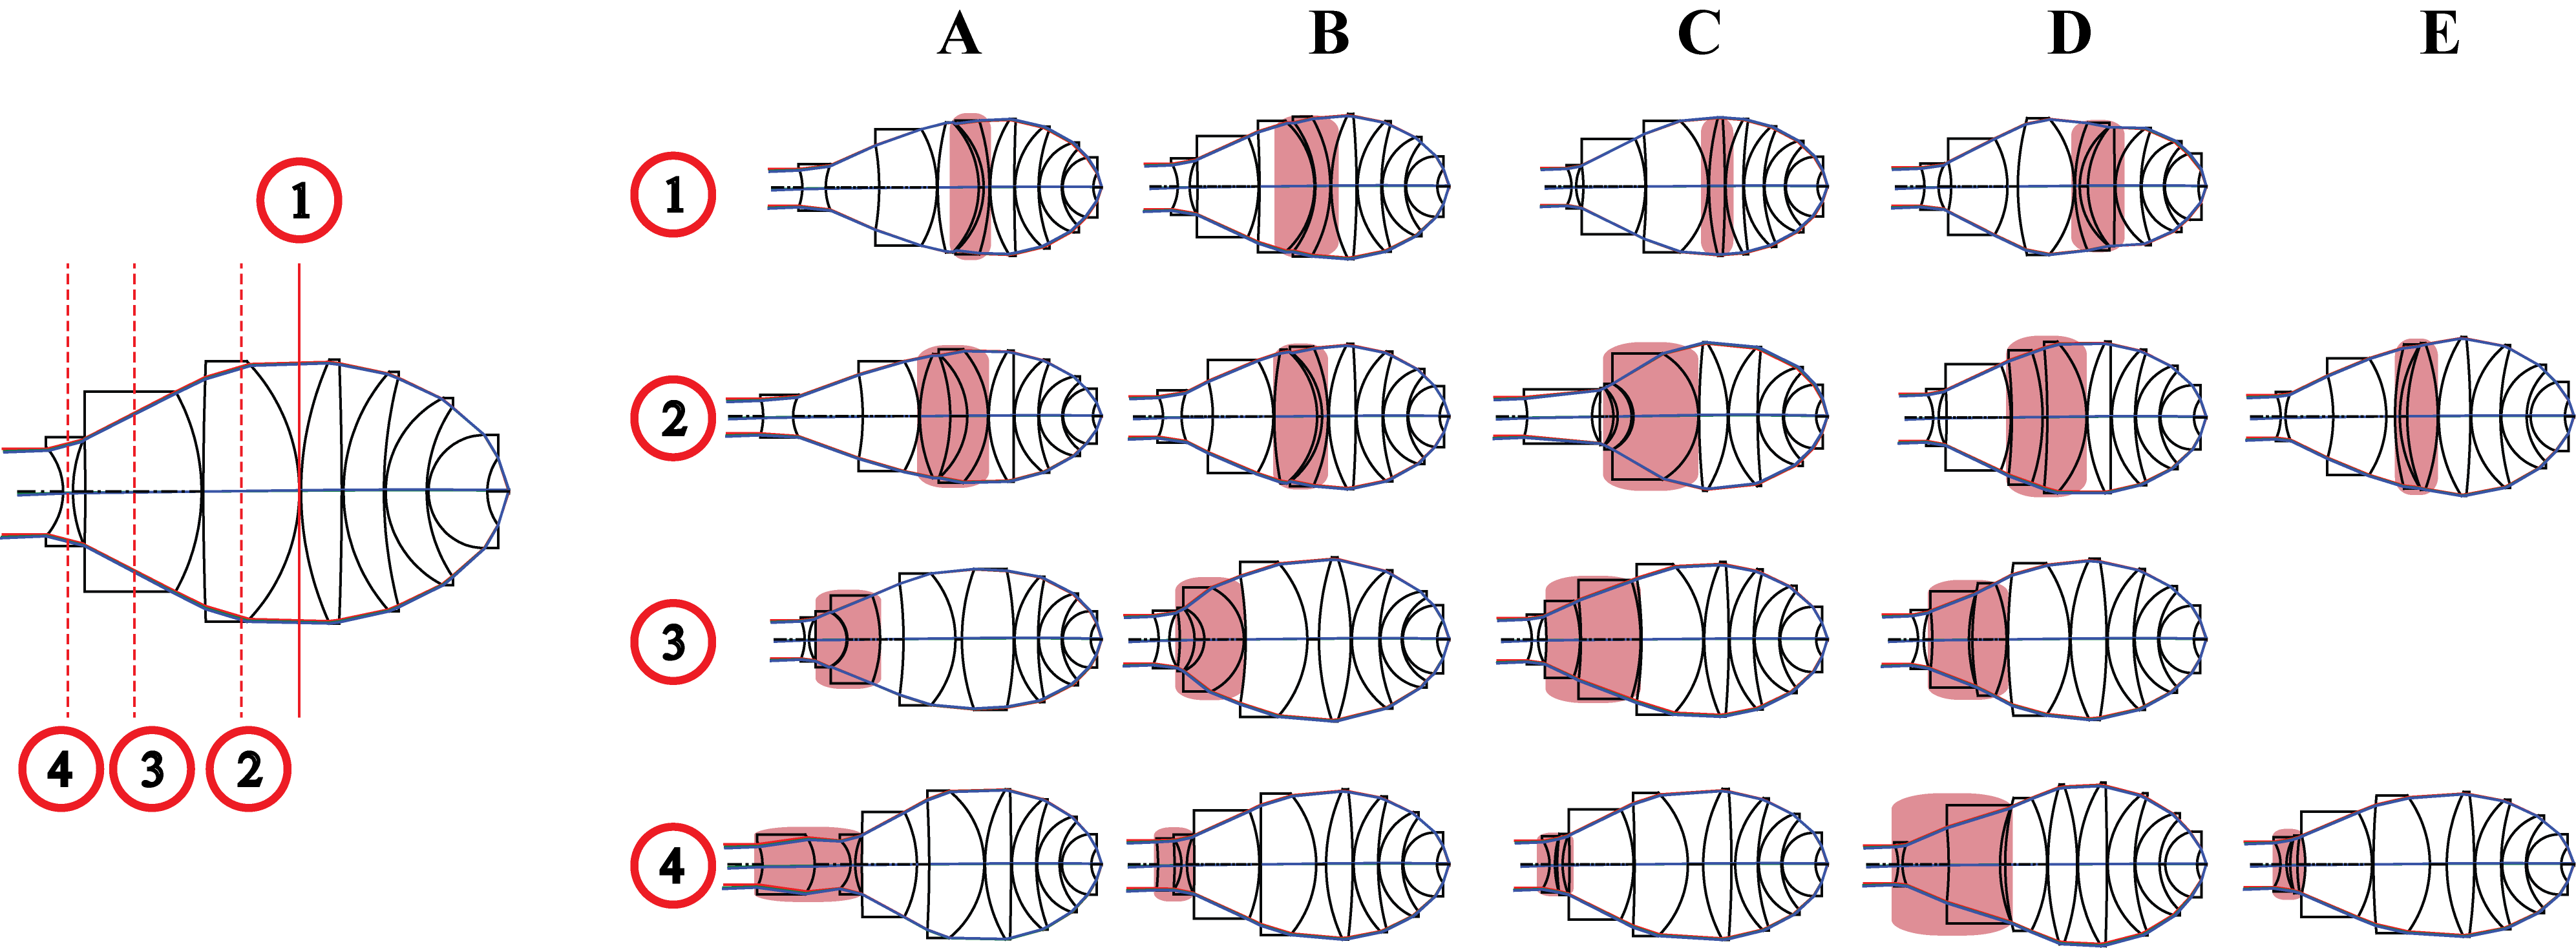
\includegraphics[width=0.96\textheight]{chapter-4/figures/vollrathSPCcaseNA.png}
  \end{adjustbox}
\end{figure}

\setlength{\arrayrulewidth}{.5mm}
\setlength{\tabcolsep}{18pt}
\renewcommand{\arraystretch}{1.2}
\begin{table}[h!]
    \centering
    \captionsetup{justification=centering}
    \caption{System performance for the systems shown in Figure \ref{fig: VollrathSPCcaseNA}}
    \label{table: vollratSPCcaseNA}
    \vspace{-1em}
    % \hspace*{-10pt} %adjusting the position of the plot(table) !!!!
    \begin{adjustbox}{max width=\textwidth, center}
    \begin{tabular}{c c c c c c}
    \hline 
       & \textbf{1} & \textbf{2} & \textbf{3} & \textbf{4} & \\ 
     \midrule
    RMS WFR & 65 & 59 & 60 & 26 & \multirow{3}{*}{\textbf{A}} \\ 
    SR(0) & 0.862 & 0.942 & 0.958 & 0.998\\
    SR(0.1) & 0.829 & 0.807 & 0.808 & 0.945\\
    \midrule
    RMS WFR& 109 & 67 & 52 & 135 & \multirow{3}{*}{\textbf{B}} \\ 
    SR(0) & 0.876 & 0.941 & 0.960 & 0.604\\
    SR(0.1) & 0.378 & 0.756 & 0.847 & 0.319\\
    \midrule
    RMS WFR & 98 & 45 & 104 & 124 & \multirow{3}{*}{\textbf{C}} \\ 
    SR(0) & 0.826 & 0.989 & 0.779 & 0.661\\
    SR(0.1) & 0.505 & 0.874 & 0.540 & 0.371\\
    \midrule
    RMS WFR & 48 & 102 & 89 & 35 & \multirow{3}{*}{\textbf{D}} \\ 
    SR(0) & 0.950 & 0.828 & 0.820 & 0.993\\
    SR(0.1) & 0.859 & 0.444 & 0.625 & 0.894\\
    \midrule
    RMS WFR &  & 43 &  & 135 & \multirow{3}{*}{\textbf{E}} \\ 
    SR(0) &  & 0.982 &  & 0.789\\
    SR(0.1) &  & 0.853 &  & 0.251\\
    \hline
    \multicolumn{6}{c}{\textit{\footnotesize{RMS WFR = RMS Wavefront Error (m\textlambda); SR(0) = Strehl Ratio at 0 mm; SR(0.1) = Strehl Ratio at 0.1 mm.}}}\\
    % \vspace{-1em}
    % \multicolumn{6}{c}{\textit{\footnotesize{SR(0) = Strehl ratio at 0 mm; SR(0.1) = Strehl ratio at 0.1 mm.}}}
    \end{tabular}
    \end{adjustbox}
\end{table}

Compared to the traditional method, more than 4 times as many systems are obtained for a comparable amount of computational load with SPC than with the traditional method. Besides the good solutions which are similar to the ones obtained with the traditional method, SPC also found eight additional solution with satisfactory performance. 

\newpage
\subsubsection{Increasing the Working Distance of the Objective}
A second structural change is introduced in the case of an increase of the working distance of the original system ( the system on the left in Figure \ref{fig: vollrathNA90295}), from 0.6 mm to 2.5 mm. This requires that the first lens element on the right is aplanatic-concentric instead of plano-concentric, causing a necessary decrease of power of the first element. In order to maintain the performance, this decrease of optical power need to be compensated. This is done by increasing the optical power of the lens element after the first one and those in the middle group. With the limited number of degrees of freedom, the performance of the system strongly deteriorates. Figure \ref{fig: vollrathWD06to25} shows how the system changed after increasing the working distance from 0.6 mm to 2.5 mm. The OverAll Length (OAL) of the system increases from 25 mm to 76 mm. The diameter of the maximum element increases from 6.6 mm to 17 mm. A longer air gap emerges after the first element on the left caused by the increase of the size (diameter) of the lens elements. The third lens element from the left is compressed into a thinner element. The bending of each element still remains close to that of the original system. Table \ref{table: vollrathWDchange} gives the change of the performance with the increase of the working distance. 

\begin{figure}[h!]
    \centering
    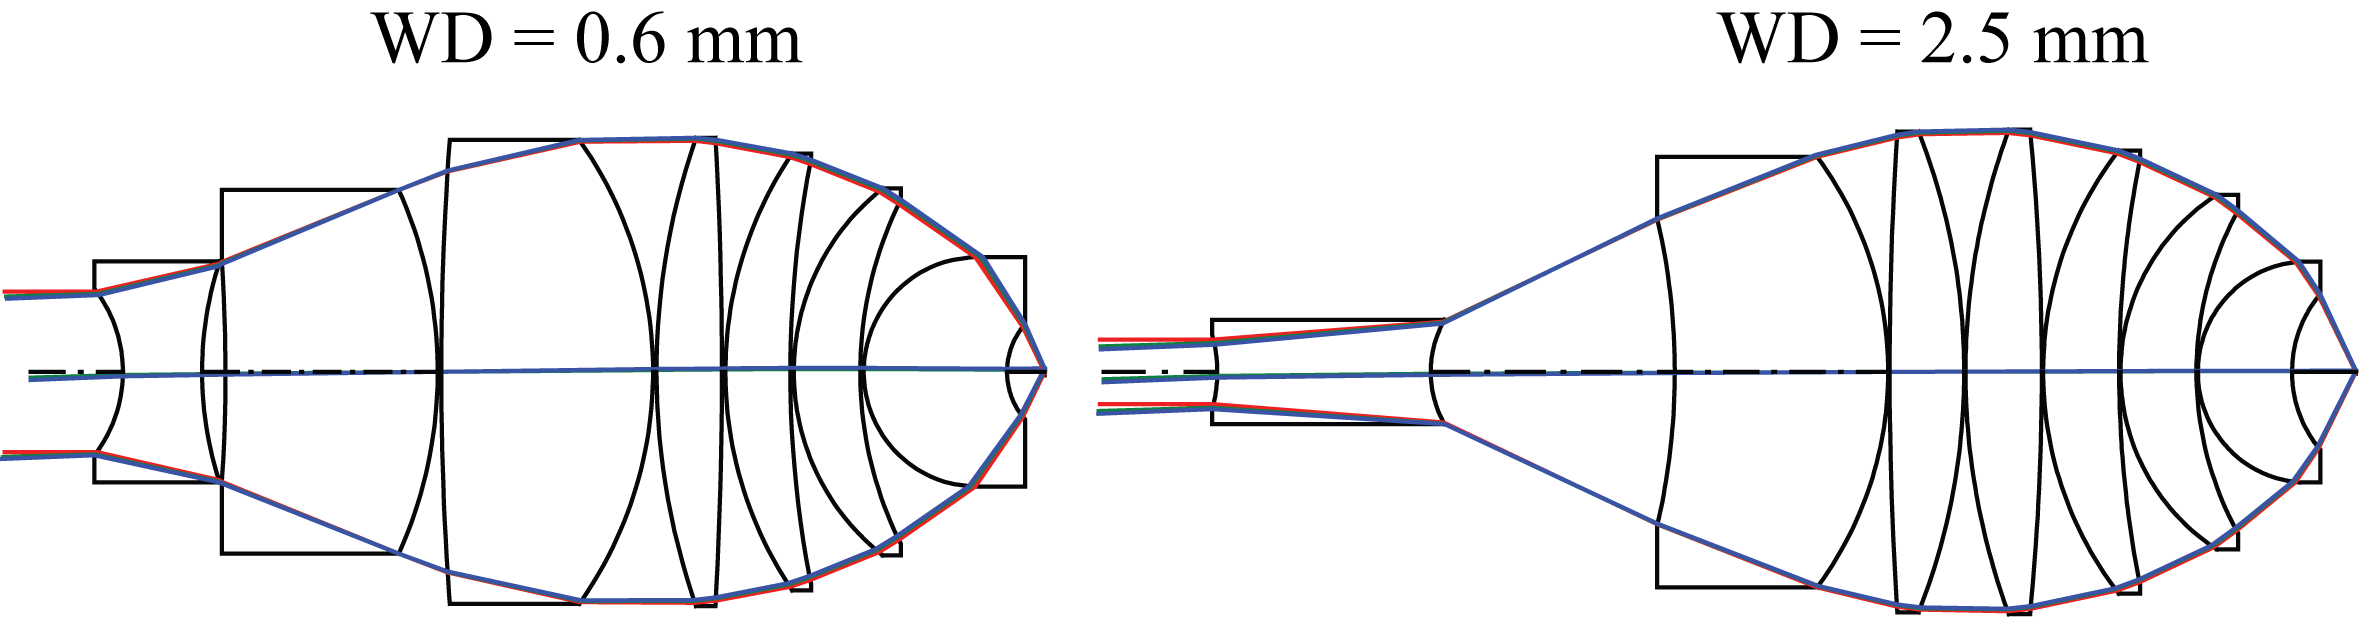
\includegraphics[width=0.75\textwidth]{chapter-4/figures/Vollrath_WD06TO25.png}
    \caption{Change of the system shape after the increasing of the working distance from 0.6 mm to 2.5 mm.}
    \label{fig: vollrathWD06to25}
\end{figure}

%table template
\setlength{\arrayrulewidth}{.5mm}
\setlength{\tabcolsep}{18pt}
\renewcommand{\arraystretch}{1.2}
\begin{table}[h!]
    \centering
    \captionsetup{justification=centering}
    \caption{Change of the system performance with increasing working distance}
    \label{table: vollrathWDchange}
    \vspace{-1em}
    \begin{tabular}{ c c c }
    \hline 
     Working distance (WD, mm) & 0.6 & 2.5\\ 
     \cmidrule{2-3}
    RMS wavefront error (m\textlambda) & 49 & 135  \\ 
    Strehl ratio at 0 mm & 0.976 & 0.254\\
    Strehl ratio at 0.1 mm & 0.849 & 0.019\\
    \hline
    \end{tabular}
\end{table}

To compensate for the decreased optical power of the first element, a common practice to introduce changes to the system for system improvement is to introduce a structural change in the middle or front group. By splitting or adding lens elements, newly added degrees of freedom will help to correct the aberrations. Two insertion positions and one splitting position were chosen for adding new degrees of freedom to the system. Figure \ref{fig: vollrathWDTrad} presents the results of the three operations: two insertions led to the same solution; the splitting shows a different system with good performance. The data of the system are listed in Table \ref{table: vollrathWDTrad}.

\setlength{\arrayrulewidth}{.5mm}
\setlength{\tabcolsep}{18pt}
\renewcommand{\arraystretch}{1.2}
\begin{table}[h!]
    \centering
    \captionsetup{justification=centering}
    \caption{System performance for the systems shown in Figure \ref{fig: vollrathWDTrad}}
    \label{table: vollrathWDTrad}
    \vspace{-1em}
    % \hspace*{-10pt} %adjusting the position of the plot(table) !!!!
    \begin{adjustbox}{max width=\textwidth, center}
    \begin{tabular}{c c c}
    \hline 
     No. & \textbf{1 \& 2} & \textbf{3}  \\ 
     \midrule
    RMS Wavefront Error (m\textlambda) & 100 & 41 \\ 
    Strehl Ratio at 0 mm & 0.833 & 0.975 \\
    Strehl Ratio at 0.1 mm & 0.507 & 0.902 \\
    \hline
    \end{tabular}
    \end{adjustbox}
\end{table}

\newpage % adjust page arrangement

\begin{figure}[h!]
    \centering
    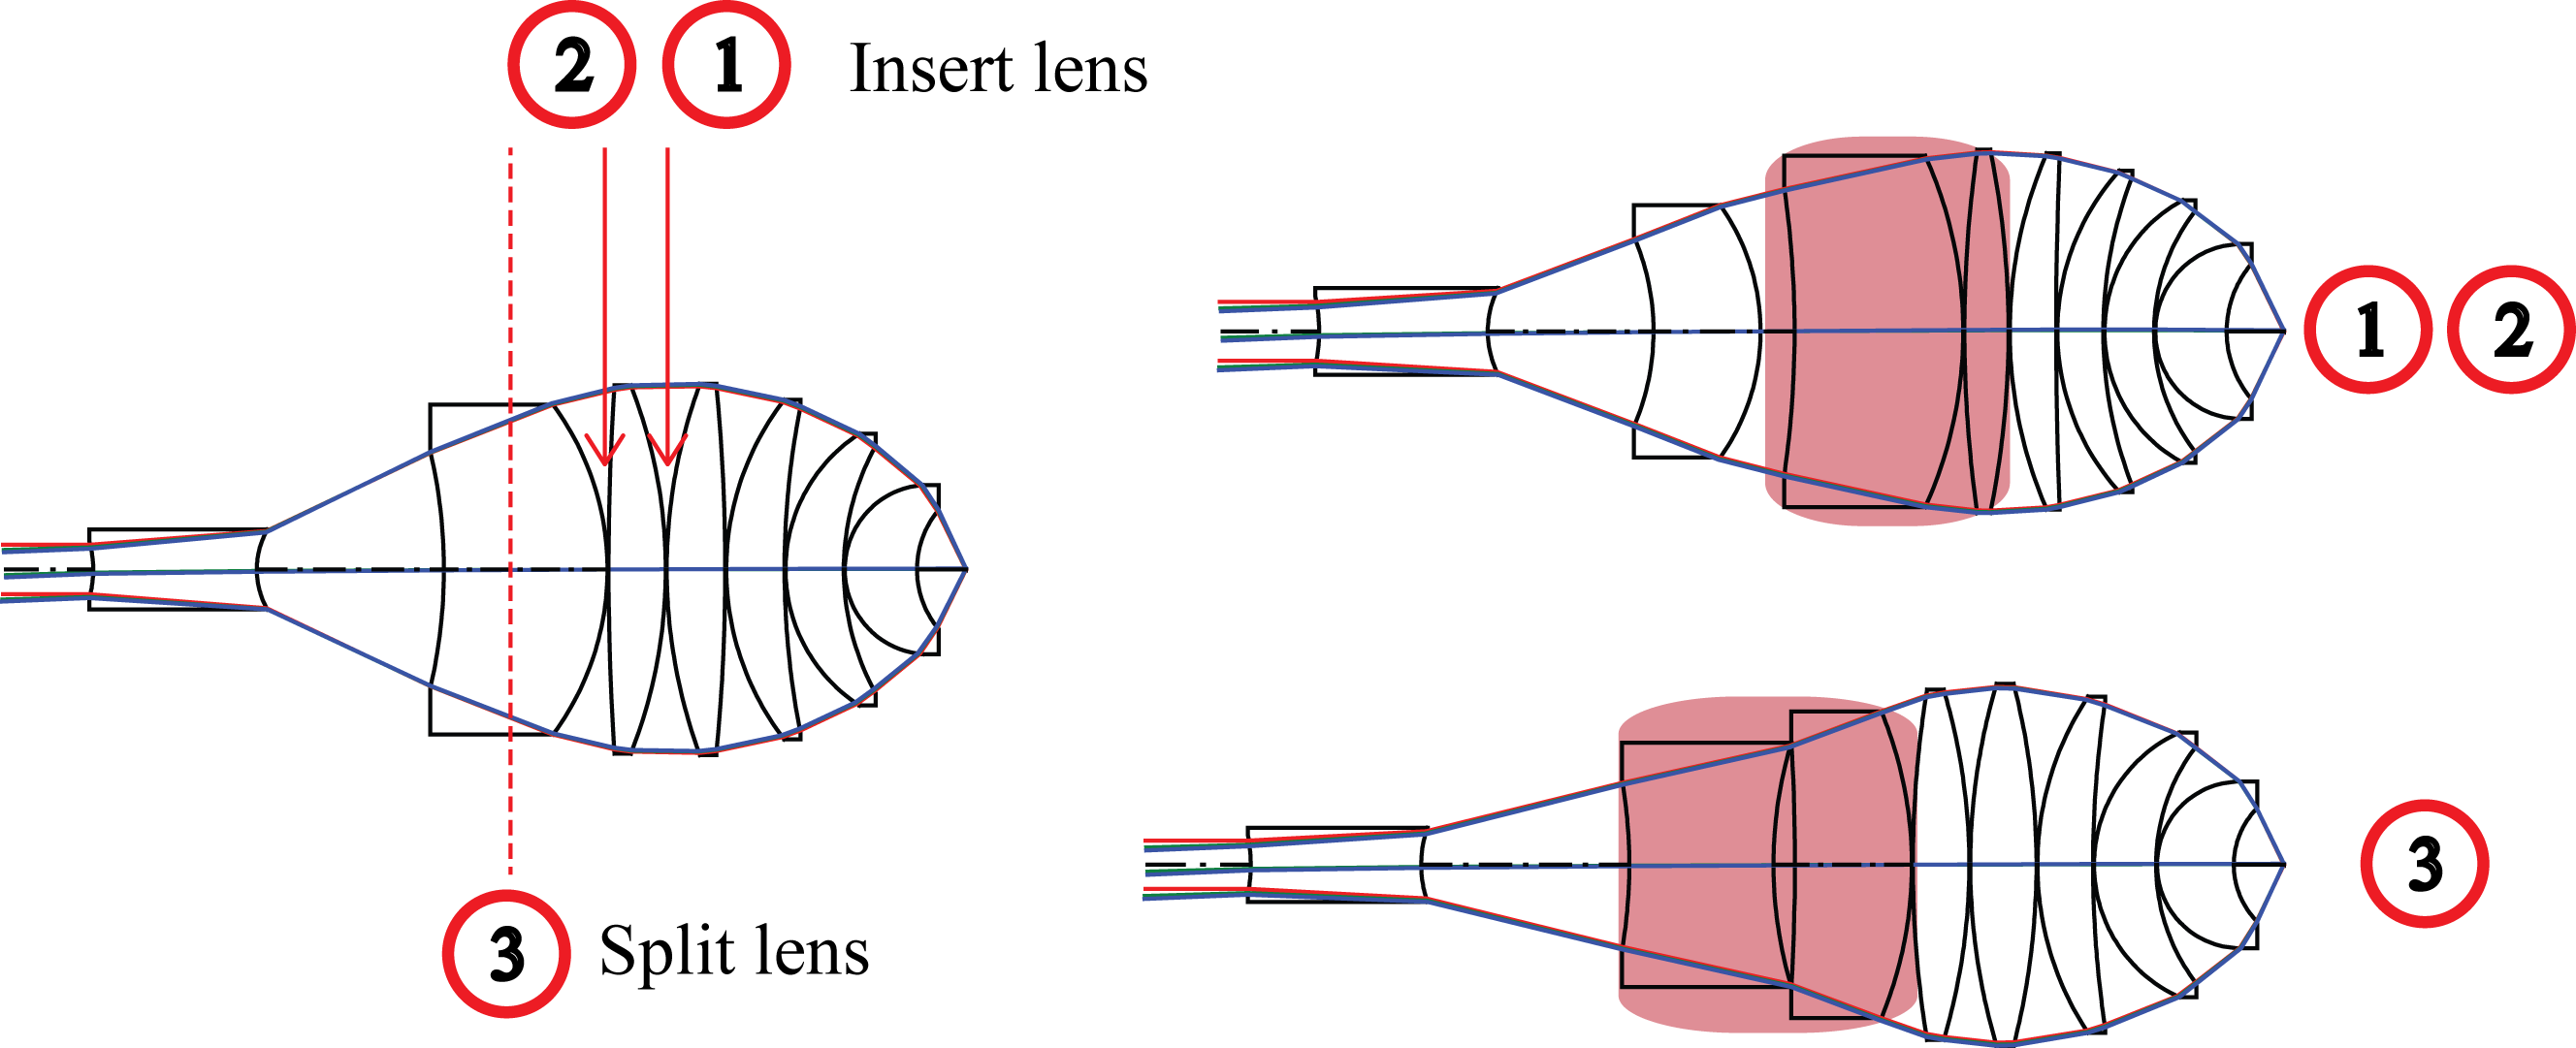
\includegraphics[width=0.6\textwidth]{chapter-4/figures/vollrathWDTrad.png}
    \caption{Introducing structural change in the traditional way to improve the performance of the system. Insertions at position \textcircled{\scriptsize{1}} and \textcircled{\scriptsize{2}} result in the same solution. }
    \label{fig: vollrathWDTrad}
\end{figure}
SPC scans are applied at the same positions where a lens is added or split. The result is shown in Figure \ref{fig: vollrathWDSPC}. From three operations of SPC, ten systems were obtained. The performance of these 10 systems is listed in Table \ref{table: vollrathWDcase}. Out of the ten systems, six have low wavefront RMS value and Strehl ratio above 0.8 for both fields. By carefully examing the system plots in Figure \ref{fig: vollrathWDSPC}, it is seen that some systems have similar system shapes. For example, systems \circled{1}B, \circled{2}B, and \circled{3}B have very close bending for each lens element. The differences among the three are in the lens thickness and air space variations. System \circled{2}A and system \circled{3}A also are very similar. When compared with the results from the conventional approach, system \circled{3}D in Figure \ref{fig: vollrathWDSPC} and system \circled{3} in Figure \ref{fig: vollrathWDTrad} are comparable solutions (especially with respect to the front group on the right). Both systems have Strehl ratio above 0.9 and have close wavefront RMS (39 and 41 $m\lambda$, where SPC constructed one has slightly better performance).

In this example where the working distance is increased, with the conventional approach, two systems were obtained with three operations. One out of three (33\%) has good performance. Using SPC, ten systems were obtained with the same amount of operations as needed in the traditional approach. Six out of ten (60\%) give satisfactory performance. 

\begin{figure}[h!]
    \centering
    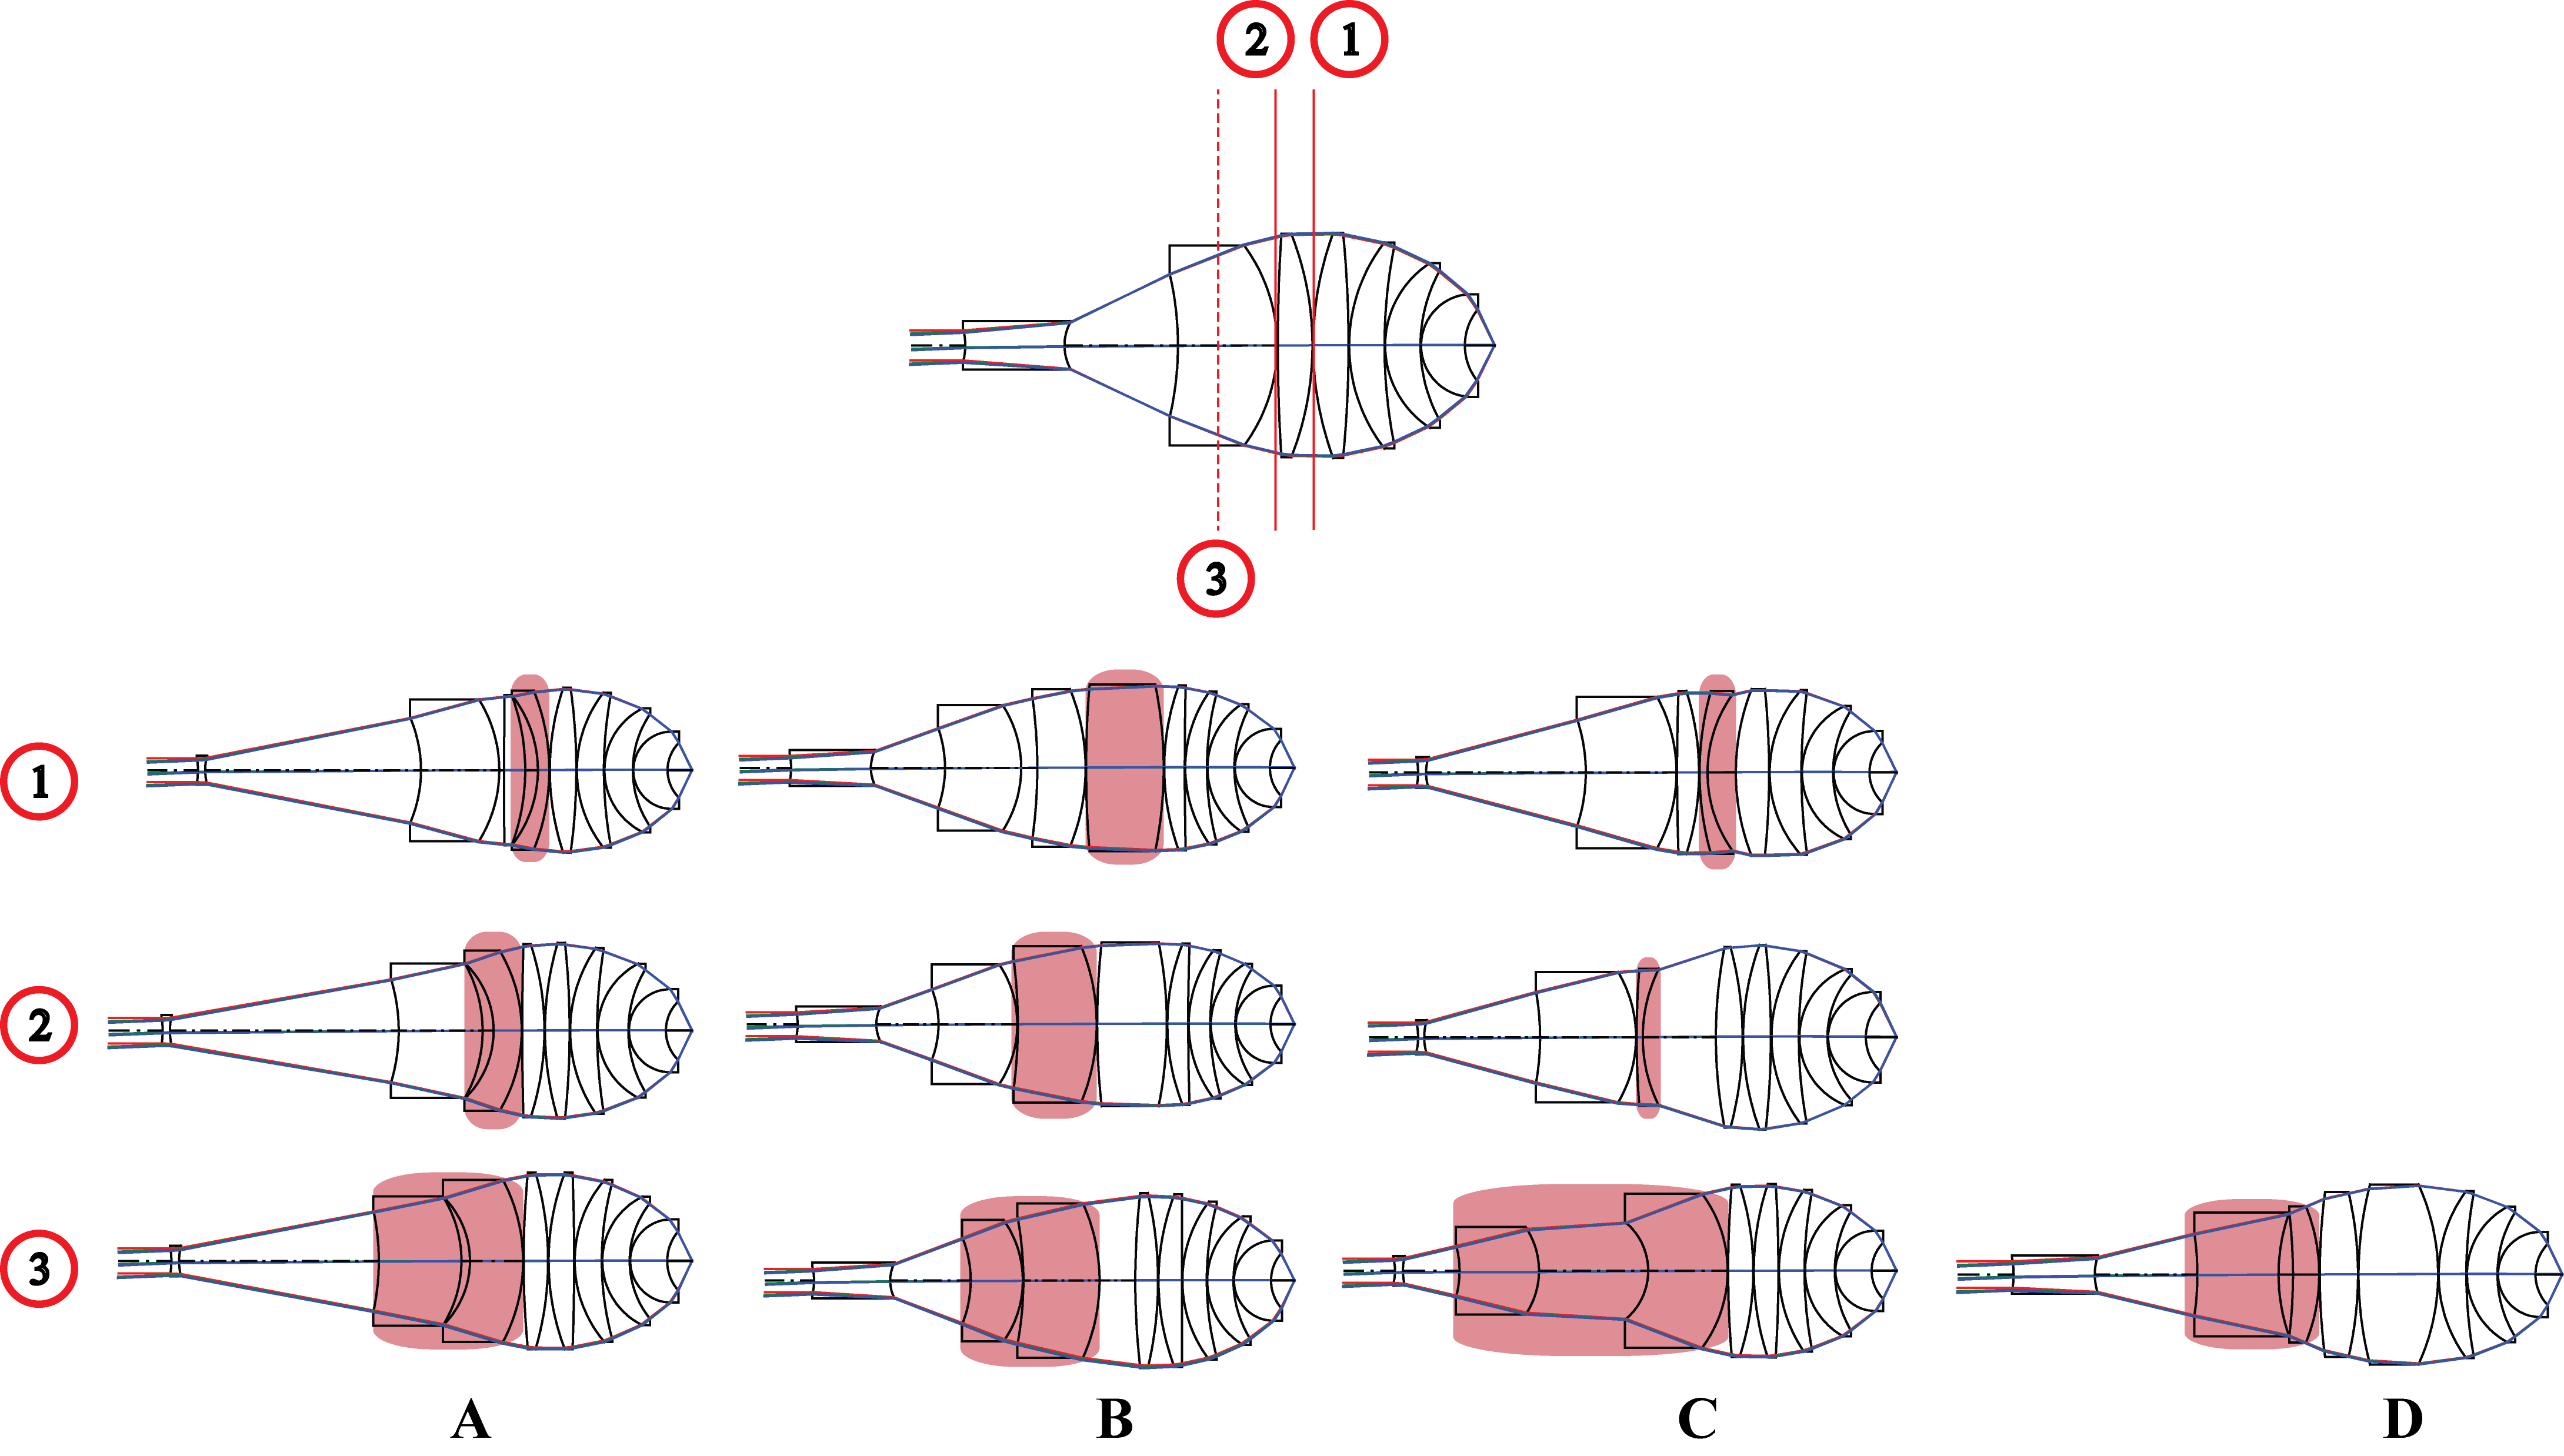
\includegraphics[width=\textwidth]{chapter-4/figures/vollrathWDSPC.png}
    \caption{Systems obtained using three SPC scans performed at the marked locations. Solid lines (\textcircled{\scriptsize{1}} and \textcircled{\scriptsize{2}}) indicate insertion of glass null-element. Dashed line (\textcircled{\scriptsize{3}}) indicates insertion of air null-element. In total, ten systems were obtained. The modified parts are highlighted.}
    \label{fig: vollrathWDSPC}
\end{figure}

\setlength{\arrayrulewidth}{.5mm}
\setlength{\tabcolsep}{18pt}
\renewcommand{\arraystretch}{1.2}
\begin{table}[h!]
    \centering
    \captionsetup{justification=centering}
    \caption{System performance for the systems shown in Figure \ref{fig: vollrathWDSPC}}
    \label{table: vollrathWDcase}
    \vspace{-1em}
    % \hspace*{-10pt} %adjusting the position of the plot(table) !!!!
    \begin{adjustbox}{max width=\textwidth, center}
    \begin{tabular}{c c c c c}
    \hline 
       & \textbf{1} & \textbf{2} & \textbf{3} & \\ 
     \midrule
    RMS WFR & 55 & 49 & 60 & \multirow{3}{*}{\textbf{A}} \\ 
    SR(0) & 0.952 & 0.976 & 0.946  \\
    SR(0.1) & 0.835 & 0.863 & 0.807  \\
    \midrule
    RMS WFR & 133 & 101 & 179 & \multirow{3}{*}{\textbf{B}} \\ 
    SR(0) & 0.645 & 0.779 & 0.410  \\
    SR(0.1) & 0.309 & 0.511 & 0.131  \\
    \midrule
    RMS WFR & 95 & 43 & 41 & \multirow{3}{*}{\textbf{C}} \\ 
    SR(0) & 0.732 & 0.971 & 0.983  \\
    SR(0.1) & 0.642 & 0.901 & 0.896 \\
    \midrule
    RMS WFR &  & & 39 & \multirow{3}{*}{\textbf{D}} \\ 
    SR(0) &  &  & 0.978 \\
    SR(0.1) &  &  & 0.910 \\
    \hline
    \multicolumn{5}{c}{\textit{\footnotesize{RMS WFR = RMS Wavefront Error (m\textlambda); SR(0) = Strehl Ratio at 0 mm; SR(0.1) = Strehl Ratio at 0.1 mm.}}}\\
    \end{tabular}
    \end{adjustbox}
\end{table}

\newpage

\subsection{Further Consideration when Applying SPC to Complex System}

When working with complex systems, there are some additional factors which have to be considered in order to properly use SPC. These additional factors usually appear because of the increasing complexity of multi-variable optimization and the design approaches in complex lens design. Increased complexity here refers to the increased number of variables used. 

\begin{figure}[h!]
    \centering
    \includegraphics[width=\textwidth]{chapter-4/figures/vollrath_optcyc.png}
    \caption{SPC scan curves at the same position with different numbers of optimization cycles}
    \label{fig: vollrath_optcyc}
\end{figure}

\subsubsection{Quality of the Local Minimum and the SPC Scan Curve}
One of the known issues occurring with complex systems is that often when the number of variables increases, the optimization basin around the local minimum becomes a vast shallow region where absolute convergence can not be achieved and no proper local minimum can be found, even when very large number of optimization cycles are performed \cite{Brixner81}. It is observed that, when the local minima in $N$ dimensional space were not computed accurately, there are problems finding the saddle points in the $N+2$ dimensional space with the SPC method. An example is given for the case where the working distance of the microscope objective is increased. Before proceeding with the SPC scan, the system has to be well-optimized to a local minimum. The merit function is defined by the default transverse ray aberration in CODE V. Two weight constraints were used: an EFL constraint of 2.5 mm and an edge thickness constraint of 2.5 mm on the first surface from the right, both with a weight of 0.01. Fourteen curvatures of the surfaces were used as variables. A threshold for the improvement of the merit function was defined as a criteria to stop the optimization. The threshold was set as $1^{-15}$, which means that when the decrease of the merit function value is less than $1^{-15}$, the optimization will stop. 
 
Without human interference, the optimization for this system ran with 5500 cycles (or optimization iterations), and it took 20 minutes (CPU: Dual-core 3.20GHz) to finish. This implies that there must be a very shallow region around the local minimum where the value of the gradient is close to zero. In the practice of lens design, the designer probably will manually stop the optimization before it runs for 5500 cycles. However, Figure \ref{fig: vollrath_optcyc} demonstrates that the decision of when to stop the optimization affects the number of saddle points that are found. The SPC scan was performed on the fourth surface from the left, as shown in Figure \ref{fig: vollrath_optcyc}. In the same figure, different scan curves are plotted with different numbers of optimization cycles applied. Up to 2500 cycles, there is no crossing between the SPC scan curve and the "$0$ " horizontal axis. From 5500 cycles up to 30,000 cycles, the scan curves are closely positioned giving very similar values of the saddle points. From the zoomed plot in Figure \ref{fig: vollrath_optcyc}, the five curves intersecting the horizontal axis are from 0.00466 to 0.00472. The example shows that, to properly perform SPC scan, it is necessary to compute the local minimum very accurately, even if the local optimization may take many more steps than usual. In this case, with insufficient optimization, two saddle points may be missed. Consequently, the three systems in row \circled{2} (the second row) of Figure \ref{fig: vollrathWDSPC} would not be obtained. 

\subsubsection{Choice of Weights and Constraints}
Other aspects which also require attention concerning SPC scans are the choices of constraints and their weights used in the merit function. As explained in Section \ref{Constraints in optical design software}, using weighted function (or penalty function, essentially identical to weighted function) for constraints implementation is compatible with SPC scan. As a result, adding weighted constraints alters the topography of the optimization landscape.  In this section, we explain the choice of constraints and their weights, change the shape of the SPC scan curve significantly. In some cases, the number of obtained saddle points varies for different combinations of constraints and weights. 

In Figure \ref{fig: vollrath_consdif}, the scan curves of two choices of constraints are shown. Case - 1 (the red-coloured line in Figure \ref{fig: vollrath_consdif}) was only with an effective focal length constraint, and Case-2 was using both an effective focal length constraint and an edge thickness constraint. As seen in the figure, the scan curve of Case-1 has six zero-crossings with the horizontal axis, whereas that of Case-2 has only two zero-crossings. 
\begin{figure}[h!]
    \centering
    \includegraphics[width=\textwidth]{chapter-4/figures/Vollrath_ConstraintDif.png}
    \caption{Change in the saddle point scan curve when different constraints are applied.}
    \label{fig: vollrath_consdif}
\end{figure}

In practice, the number of local minima is more important than the number of constructed saddle points. For the given example, Case-1 did not include the edge thickness requirement in the merit function. If this requirement is not met, it is necessary to add the constraint on the edge thickness and optimize from the minima acquired in the next step. In Case-2 the two necessary constraints on the EFL and the edge thickness are taken account of from the start, hence, the acquired minima are the final solutions. Design procedure and the obtained local minima are shown for both cases in Figure \ref{fig: vollrath_constr_flow}. For Case-1, seven local minima are acquired from six saddle points. For Case-2, three minima are obtained from two saddle points. Judging by the system shapes, the three minima from Case-2 correspond to the local minima in the set obtained in Case-1. The pairs of corresponding local minima are highlighted with different colours in Figure \ref{fig: vollrath_constr_flow}. It is seen that MA-4 and MB-2, which belong to the same system shape, have very similar merit function values. However, the two pairs MA-1, MB-1 and MA-6, MB-3 have bigger differences in their merit function values. Although the system shapes are similar, due to the complex topography of the design landscape in the case of many variables, the merit function values can be quite different. The same observation was described in \cite{PascalTriplet2009}. 


\begin{figure}[h!]
    \centering
    \includegraphics[width=\textwidth]{chapter-4/figures/Vollrath_ConstraintDif_flow.png}
    \caption{Two different design processes leading to different sets of local minima. On the left: saddle point scan with only the EFL constraint, with the edge thickness constraint applied only in the last stage. In total seven minima are obtained. On the right: SPC scan with both EFL and edge thickness constraints incorporated followed by local optimization using both constraints. This led to three local minima. Systems with similar shapes are given the same colour.}
    \label{fig: vollrath_constr_flow}
\end{figure}

In addition to the number of constraints used, the choice of the weight also affects the SPC scan curve. An example is given in Figure \ref{fig: vollrath_wt_change}, where different scan positions are chosen using the same system from the previous example. Only the EFL constraint is applied here with different weight number from 0.001 to 10. In Figure \ref{fig: vollrath_wt_change}, it is shown that when the weight is 0.001 or 10, the SPC scans produce curves that differ from those in the other three cases. Weight 0.001 gives four saddle points, weight 10 gives two saddle points, and the other three cases give three saddle points. The target value of the EFL is 2.50 mm. When a weight of 0.001 is used, the optimized system has an EFL of 2.65 mm. For a weight of 0.01, the EFL is stabilized around 2.53 mm. When the weight is larger than 0.1, the optimized system has an intended EFL of 2.50 mm. 

According to the derivation of the special case of SPC \cite{BociortSPCSexplained}, when the space between the constructed surface and another optical surface is zero (or close to zero), a saddle point can be found with the curvatures of the constructed surface identical (or similar) to that optical surface. In this example, when the weight is 0.01, 0.1 and 1, the most left and most right saddle points represent the special case saddle points. However, when the weight is too big or too small, the design landscape is altered in a way that the special case of saddle point cannot be obtained via the scan (weight 10 case missed the left one). One of the hypotheses is that there are some numerical inaccuracy when computing the local minima and saddle points with these extreme weights. More investigations are needed to understand these situations. Based on the observations in this example, for practicing the SPC, we would suggest to avoid using extreme weight values. 

From the two examples, it is seen that the way to implement the constraints affects the number of saddle points acquired from SPC. This will lead to differences in the obtained minima. Regarding the constraints applied, the example shows that starting with a simple constraint generates more saddle points than applying several constraints at the same time. It is consistent with the design rule that constraints are usually added progressively. If all constraints are added at the same time, using the Lagrange multiplier method adds multiple new variables to the optimization problem, therefore can generate more local minima and make the global optimization more difficult.  When using the weight function, there is lack of systematic knowledge on how to adjust multiple weights in one merit function. Constraints that are not massively violated should not be included in the SPC scan, but should be applied only on the resulting minima. We recommend avoiding extreme values of weight when using SPC with a merit function containing weight constraints. In general, the weights should be adapted during the design process, depending on the problem. When applying SPC, it is necessary to keep the weights the same during the application of SPC and the following local optimizations. After obtaining the local minima, the weights can be adapted when the design process is continued. 

\begin{figure}[h!]
    \centering
    \includegraphics[width=\textwidth]{chapter-4/figures/Vollrath_wt_change.png}
    \caption{Change in the saddle point scan curve when different constraint weights are applied.}
    \label{fig: vollrath_wt_change}
\end{figure}

\newpage
\section{Applying SPC to a Photo-Lithographic Objective}
Lithographic systems represent one of the most sophisticated types of optical systems nowadays. With an imaging objective consisting of more than twenty lens elements, nanometer resolution has to be realized. These systems are used in the semiconductor industry to produce integrated chips \cite{Matsuyama2006_LithoHis}, which boost all kinds of technology advances in the 21st century. 

For these kinds of complicated optical systems with a large number of variables, the number of possible solutions increases drastically. These systems suffer more easily from ray failures. Varying variables in the system can easily cause failures in ray tracing. Normally, a new design starts from an existing one, where the system specification is close to the design requirement. The system is then modified by the designer based on certain design guidelines \cite{LivshitsQA2013}\cite{Shafer1995_moreless}\cite{Cao2017_GroupDesign} or his/her own experience. Trial and error always evolves before obtaining a good solution. 

A Deep Ultra Violet (DUV) lens from an existing patent \cite{patentZeissDUV} is selected. We choose the design from the embodiment described in Figure 5 of this patent. The system parameters are given in Table 5 in the patent. We use this DUV objective as an example to demonstrate how SPC can be applied in a complex case. The DUV objective is designed to work at 193 nm wavelength. The numerical aperture is 0.85, the image height is 14.02 mm and the magnification is -0.25. The system is optimized for distortion and telecentricity. The wavefront RMS error is 3.26 $m\lambda$. The objective consists of twenty-three lens elements, where eight surfaces are aspheric. The system plot is presented in Figure \ref{fig: litho_DUV_plot}. 
\begin{figure}[h!]
    \centering
    \includegraphics[width=\textwidth]{chapter-4/figures/Litho_DUV_plot.png}
    \caption{DUV objective lens from \cite{patentZeissDUV}. It consists of, in total, twenty-three lens elements. Eight surfaces are aspheric surfaces marked by thickened line.}
    \label{fig: litho_DUV_plot}
\end{figure}

This objective has been previously studied with the special version of SPC. In the special version, no curvature scan is used. The designer decides where to insert the null-element. This is always done on an existing surface. A saddle point system is directly obtained by the way the null element is inserted \cite{BociortSPCSexplained}. Two new solutions can be obtained by optimizing from the saddle point. In the study of Marinescu\cite{OanaThesis2006}\cite{OanaOEngPart2}, examples are given to use the special version of SPC to add lenses to the original system to obtain different local minima. Afterwards, other lenses are chosen to be deleted. In this way, the system maintains similar performance with a smaller number of optical elements. However, the strategy for where to add or extract the lenses is not explained in detail. This question remains unanswered by our research, and it makes the design of large systems more complicated. Marinescu's method has two steps: 1) choose the place to add a lens with SPC; 2) choose lenses to be extracted. The design process is a combination of SPC and conventional methods. The designer needs to make the decision twice on where to add and extract the lens. In the following examples, we will show that with SPC, the designer only needs to decide once where to perform SPC to achieve performance improvement. 

The sixth lens (from the left) is chosen to be replaced using SPC following the example in Marinescu's thesis (where she chose to add a null-element next to it). The first step was to remove the chosen lens by gradually reducing the thickness of the lens while optimizing the system, at the same time to keep the system staying in the same basin of attraction. Once the thickness is reduced to zero, constraints are applied to make the element a meniscus null-element (equal curvature with zero-thickness). In this way, the element could be removed without affecting the system. In practise, the element does not need to be physically removed, since the next step is to perform an SPC scan at the same location. 

As demonstrated in the previous section, the choice of constraints in the merit function may affect the obtained result. The recommendation is to start with a relative simple merit function. The complexity of the merit function can be increased after the SPC process. A default unconstrained merit function based on wavefront aberration \footnote{In CODE V, the merit function is based on wavefront variance. It comes from the weighted combination of the optical path difference (OPD) and the X and Y wavefront slope values.} is used for the phase of the SPC scan: the variables used are only the curvatures of the spherical surfaces (thirty six variables, the last element is a plane-parallel plate). Since the air spaces and lens thicknesses are not varied and the system is already very "tight", an unconstrained optimization does not drastically change the system. With the default wavefront aberration merit function, the original system has a merit function value of 0.002915, and a wavefront aberration of 3.26 $m\lambda$. After unconstrained optimization, the merit function value becomes 0.002391, and the wavefront aberration increases to 3.53 $m\lambda$. The merit function is calculated assuming that the best focus is determined by the paraxial calculation (ideal focus plane). The wavefront aberration is given by the wavefront analysis in CODE V, which traces the real rays and determines best focus plane using the real rays. Therefore, due to the different choices of the focal planes, a decreased merit function can bring an increased wavefront aberration. The computation technique used in the merit function is aimed for facilitating the optimization. When the sixth lens element was extracted, the merit function deteriorated to 0.013822, and the wavefront aberration increased to 12.39 m\textlambda.

Performing an SPC scan at the position where the sixth lens is extracted, yielded six saddle points. These six saddle points lead to twelve minima with a zero-thickness element. After increasing the thickness, the twelve systems converge into four solutions. The reason for the convergence of the solutions is that when the thicknesses increase, local minima can encounter ray failure or merge with other local minima. An example of ray failure caused by thickness increase is explained in Figure \ref{fig:thickness_increase}. In Figure \ref{fig: litho_step1_2}, the first two steps of performing an SPC scan on the lithographic objective are illustrated.

\begin{figure}[h!]
    \centering
    \includegraphics[width=\textwidth]{chapter-4/figures/Litho_Step1_2.png}
    \caption{Step 1, Extract the selected element (highlighted); Step 2, Perform SPC at the location of the extraction (dashed line location). With the SPC scan, six saddle points were obtained which led to four local minima. }
    \label{fig: litho_step1_2}
\end{figure}

The system plots of the four new systems are shown on the left of Figure \ref{fig: litho_Step3}. The extracted and then constructed lens elements are highlighted. It is observed that the new solutions mostly differ from each other in the lenses close to the position of extraction and where the SPC scan is performed. By comparing the systems, we see that the highlighted lens and its neighbouring lens differ in the lens bending between different systems. For example, DUV-M1 has meniscus - meniscus - biconvex around the highlighted lens and DUV-M4 has meniscus - biconvex - meniscus around the highlighted lens. It is also worth noticing that there is no system identical to the original system at the top row of Figure \ref{fig: litho_Step3}. The constructed lens of DUV-M4 shows similar bending shape as the original system, however, the neighbouring right element has a meniscus shape which is different from the plano-convex shape in the original system. One can not expect to find a system that is identical to the original system because the solutions are obtained by optimization without constraints. The next step (Step 3) as shown in Figure \ref{fig: litho_Step3} is to add constraints to the merit function and minutely optimize every solution obtained from the SPC scan. Constraints like magnification, distortion control and edge thickness etc. were added to the original merit function. Weights and number of constraints were tailored for each system in order to reach a solution which has good performance as while as fulfill the constraints. Extra variables such as aspheric coefficients, air spaces and lens thicknesses were also used in the last stage. The corresponding solutions are listed on the right side of Figure \ref{fig: litho_Step3} as DUV M1' - M4'. Judging from the system plots, it is seen that most of the differences between the systems are still localized around the constructed element. Compared to the previous stage, the major change of the further optimized solutions are the thicknesses of the lenses and the air spaces between them. This implies that in the fine tuning optimization stage, the system stays in the same basin of attraction when the curvature variables are varied.


\begin{figure}[h!]
    \centering
    \includegraphics[width=\textwidth]{chapter-4/figures/Litho_SPC_minima_listed.png}
    \caption{Step 3 of performing SPC on a lithographic objective: applying constraints to the systems obtained from the SPC and further optimize the systems using more variables (thickness, aspheric terms, etc.). The optimized systems are evaluated on their performances.}
    \label{fig: litho_Step3}
\end{figure}

In Table \ref{table: Litho_final_solution}, the performances of the four optimized solutions are listed. While minimizing the wavefront aberration (in RMS), the distortion and the telecentricity are controlled at the same time. Among the four new solutions, DUV-M3' shows better wavefront RMS (29$\%$ better than the orignal), distortion (16\text{\%}), and telecentricity at the image side (94$\%$). The telecentricity at the object side is worse than the original one (15$\%$). The other three new solutions show some mixed performances, with some properties better than the original system, but others worse. For a practical case, more properties have to be considered in designing a lithographic system, e.g. thermal sensitivity, manufacturability and cost. In our example, the assessing criteria have been limited to those mentioned above. The results show that with SPC and the design flow used, new solutions in a complex lithographic system can be systematically found. In the example discussed, systems with better and worse performance as compared to the original, are obtained. 

\setlength{\arrayrulewidth}{.5mm}
\setlength{\tabcolsep}{18pt}
\renewcommand{\arraystretch}{1.2}
\begin{table}[h!]
    \centering
    \captionsetup{justification=centering}
    \caption{Performance of the optimized solutions shown in Figure \ref{fig: litho_Step3}}
    \label{table: Litho_final_solution}
    \vspace{-1em}
    % \hspace*{-10pt} %adjusting the position of the plot(table) !!!!
    \begin{adjustbox}{max width=\textwidth, center}
    \begin{tabular}{c c c c c}
    \hline 
       & \textbf{Wavefront RMS (m\textlambda)} & \textbf{Distortion (nm)} & \textbf{Object Side Telecentricity* (mrad)} & \textbf{Image Side Telecentricity* (mrad)} \\ 
     \midrule
    Original & 3.26 & <1.00 & <14.36 & <19.18 \\ 
    \midrule
    DUV-M1' & 2.96 & <1.62 & <17.60 & <17.31 \\ 
    \midrule
    DUV-M2' & 3.36 & <1.43 & <17.98 & <5.84 \\ 
    \midrule
    DUV-M3' & 2.32 & <0.84 & <16.56 & <1.15 \\ 
    \midrule
    DUV-M4' & 9.91 & <2.39 & <57.01 & <10.05\\
    \hline
    \small* 'Telecentricity' here means the deviation from telecentricity.
    \end{tabular}
    \end{adjustbox}
\end{table}


\section{Conclusion}
In this chapter, multiple examples are given to demonstrate how SPC can be applied in practical lens designs. It is recommended to integrate the SPC method with conventional strategies. In this way, more solutions can be effectively produced and from them the designer should then choose the best. In the example of a wide-angle lens, where the system is divided into two groups, we show that SPC can be applied to the individual group of lenses or to the wide-angle lens combined from the two groups of lenses. Applying SPC in this wide-angle lens design helps to produce alternative solutions in the landscape. For complex system like the UV microscope objective, guided by the designer's knowledge, SPC shows better efficiency than the conventional approaches in terms of obtaining good solutions. In order to design a lithographic objective with multiple constraints, it is discussed how SPC can be integrated in a two-step design process. New solutions with local changes are obtained with mixed performances in the sense that the obtained systems, compared to the original system, are better in some aspects and worse in others. 

With the wide-angle lens, detailed steps for applying the SPC to switch to new solutions are given. The basin plots in Figure \ref{fig:basins} reveal that in some cases the obtained minima depend on the choice of the optimization starting point around the saddle point. This dependency can be a property of the design landscape, or it can be caused by the numerical configuration (e.g. choices of the damping factor) of the local optimizer. Further research is necessary to understand this phenomenon. For the given example, this dependency between the starting point and the local minima with zero-thickness element did not influence the final results after increasing the thickness for the zero-thickness minima (Table \ref{table: scanline}).

Factors that will alter the SPC scan curve are investigated. These factors are: 1) When the number of variables increases (fourteen for the UV microscope objective), a shallow local minimum should be very well optimized to ensure that the correct SPC scan curve is obtained; 2) When constraint type and weights are varied, the corresponding SPC scan curves are different. We observe that more constraints and more rigid weights (leading to a stressed system) result in fewer saddle points than fewer constraints and more flexible weights (which leads to a relaxed system). Therefore, it is recommended to implement only the necessary constraints at the SPC scan stage. Extreme values of these constraints should also be avoided. It is better to add the other constraint later in the design process.

In conclusion, to design a complex system, applying SPC following the guidelines presented in this chapter will help to generate (intermediate) solutions effectively. When implementing the SPC method in a software package to serve as a lens optimization tool, the cases discussed in this chapter should be taken into account (e.g. automatically verify the SPC scan curve stability) to assist the design process.  


\references{dissertation}


\chapter{Write your title} %% change
\label{chapter_x} %% change
\graphicspath{ {./chapter-xxx/figures/} }  %% change
\captionsetup[figure]{labelfont=bf}
\captionsetup{margin=1.5em}
\captionsetup[table]{labelfont=bf}
%% The following annotation is customary for chapter which have already been
%% published as a paper.
\blfootnote{Parts of this chapter have been published in Optics Express \textbf{25}, 32474 (2018) \cite{HouSMS2018}.}

%% It is only necessary to list the authors if multiple people contributed
%% significantly to the chapter.
%\authors{Albert {\titleshape Einstein}}

%% The '0pt' option ensures that no extra vertical space follows this epigraph,
%% since there is another epigraph after it.
% \epigraph[0pt]{
%   A journey of a thousand miles begins with a single step
% }{Laozi}

% \epigraph{
%     Sample quotes
% }{author}

% \begin{abstract}
% Previous researches have shown that different solutions of the optical system can be found using saddle point based method for some simplified cases\cite{PascalTriplet2009}. It is important, however, to study whether the saddle point based method still perform well in practical lens design problems. To study this, we chose to start with a relative simple example.
% \end{abstract}

% %% Start the actual chapter on a new page.
% \newpage

\noindent This document is intended to be both an example of the TU Delft dissertation template for \LaTeX, as well as a short introduction to its use. It is not intended to be a general introduction to \LaTeX{} itself,\footnote{We recommend \url{http://en.wikibooks.org/wiki/LaTeX} as a reference and a starting point for new users.} and we will assume the reader to be familiar with the basics of creating and compiling documents.

Instructions on how to use this template under Windows and Linux, and which \LaTeX{} packages are required, can be found in \texttt{README.txt}.

%%%%%%%%%%%%%%%%%%%%%%%%%%%%%%%%%%%%%%%%%%% Section 1 %%%%%%%%%%%%%%%%%%%%%%%%%%%%%%%%%%%%%%%
\section{Document Structure}

\dropcap{S}{ince} a dissertation is a substantial document, it is convenient to break it up into smaller pieces. In this template we therefore give every chapter its own file. The chapters (and appendices) are gathered together in \texttt{dissertation.tex}, which is the master file describing the overall structure of the document. \texttt{dissertation.tex} starts with the line

%% We need an empty line before the quote environment to work around a bug in
%% the lettrine package, from which the drop command is derived.
\begin{quote}
\texttt{\textbackslash documentclass\{dissertation\}}
\end{quote}
which loads the dissertation template. The template is based on the \LaTeX{} \texttt{book} document class and stored in \texttt{dissertation.cls}. The document class accepts several comma-separated options. By default, hyperlinks are shown in cyan, which is convenient when reading the dissertation on a computer, but can be expensive when printing. They can be turned black with the \texttt{print} option. This will also turn the headers dark gray instead of cyan. Moreover, it will add a 3~mm bleed around the page including crop marks. This will help the printer with the thumb indices, since they run right up to the page borders. Finally, the \texttt{nativefonts} option can be used to override the automatic font selection (see below).

A dissertation is a big document, which makes it easy to miss warnings about the layout in the \LaTeX{} output. In order to locate problem areas, add the \texttt{draft} option to the \texttt{\textbackslash documentclass} line. This will display a vertical bar in the margins next to the paragraphs that require attention.

The contents of the dissertation are included between the \texttt{\textbackslash begin\{document\}} and \texttt{\textbackslash end\{document\}} commands, and split into three parts by
\begin{enumerate}
\item\texttt{\textbackslash frontmatter}, which uses Roman numerals for the page numbers and is used for the title page and the table of contents;
\item\texttt{\textbackslash mainmatter}, which uses Arabic numerals for the page numbers and is the style for the chapters;
\item\texttt{\textbackslash appendix}, which uses letters for the chapter numbers, starting with `A'.
\end{enumerate}
The title page is defined in \texttt{title.tex} in the \texttt{title} folder and included verbatim with \texttt{\textbackslash include\{title/title\}},\footnote{Note that it is not necessary to specify the file extension.} (see below). Additionally, it is possible to include a preface, containing, for example, the acknowledgements. An example can be found in \texttt{preface.tex}. The table of contents is generated automatically with the \texttt{\textbackslash tableofcontents} command. Chapters are included after \texttt{\textbackslash mainmatter} and appendices after \texttt{\textbackslash appendix}. For example, \texttt{\textbackslash include\{chapter-1/chapter-1\}} includes \texttt{chapter-1.tex}, which contains this introduction.

\section{Title Page}

\dropcap{T}{he} title pages are defined in \texttt{title/title.tex}, which you will have to modify according to your needs. Note that these pages are subject to the requirements of the \emph{promotieregelement} and cannot be changed at will. Apart from the names and dates, most of the Dutch text is dictated literally.

Since the thesis title and name of the author appear several times throughout the document (on the title page, but also in, \emph{e.g.}, the preface and cv), special commands are provided so they only have to be specified once. The title (and optional subtitle) can be specified with

\begin{quote}
\texttt{\textbackslash title[Optional subtitle]\{Title\}}
\end{quote}
The name of the author is specified with
\begin{quote}
\texttt{\textbackslash author\{First name\}\{Last name\}}
\end{quote}
Note that the first and last name are separate arguments, since they may be printed in different font shapes. The \texttt{\textbackslash title} and \texttt{\textbackslash author} commands also ensure that the title and author appear in the metadata of the final PDF.

See \texttt{title/title.tex} for detailed documentation on the comment and layout of the title pages. Logos of institutes that have contributed financially to the dissertation may be included on reverse side of the title page. A few example logos can be found in the \texttt{title/logos} folder.

\section{Chapters}

\dropcap{E}{ach} chapter has its own file. For example, the \LaTeX{} source of this chapter can be found in \texttt{chapter-1.tex}. A chapter starts with the command

\begin{quote}
\texttt{\textbackslash chapter\{Chapter title\}}
\end{quote}
This starts a new page, prints the chapter number and title and adds a link in the table of contents. If the title is very long, it may be desirable to use a shorter version in the page headers and the table of contents. This can be achieved by specifying the short title in brackets:

\begin{quote}
\texttt{\textbackslash chapter[Short title]\{Very long title with many words which could not possibly fit on one line\}}
\end{quote}
Unnumbered chapters, such as the preface, can be created with \texttt{\textbackslash chapter*\{Chapter title\}}. Such a chapter will not show up in the table of contents or in the page header. To create a table of contents entry anyway, add
\begin{quote}
    \texttt{\textbackslash addcontentsline\{toc\}\{chapter\}\{Chapter title\}}
\end{quote}
after the \texttt{\textbackslash chapter} command. To print the chapter title in the page header, add
\begin{quote}
    \texttt{\textbackslash setheader\{Chapter title\}}
\end{quote}

If (parts of) the chapter have already been published elsewhere, it is customary to add a reference. This can be done with the special unnumbered footnote command \texttt{\textbackslash blfootnote}. For example,

\begin{quote}
\texttt{\textbackslash blfootnote\{Parts of this chapter have been published in Annalen der Physik \textbackslash textbf\{324\}, 289 (1906) \textbackslash cite \{Einstein1906\}.\}}
\end{quote}
generates the footnote at the beginning of this chapter. Because this footnote is unnumbered, the \texttt{hyperref} package may throw a warning, which safely be ignored.

If multiple people have contributed significantly to this chapter, they can be lister with the \texttt{\textbackslash authors} command. This can be followed by a quotation using \texttt{\textbackslash epigraph} as shown above. Finally, it is customary for a dissertation to include an abstract for every chapter (except perhaps the introduction). This can be accomplished with the \texttt{abstract} environment. The abstract should be followed by \texttt{\textbackslash newpage} to start the chapter text on a new page.

In a dissertation, each chapter has its own list of references. These can be generated with the special command \texttt{\textbackslash references\{dissertation\}} from \texttt{dissertation.bib} at the end of the chapter. Note that this means that you need to run a command like \texttt{bibtex chapter-1/chapter-1} for each chapter. The bibliography style is specified in \texttt{dissertation.bst}, which is a modified version of \texttt{apsrev4-1.bst} (from REVTeX) designed to also display the titles of referenced articles. The template will automatically generate clickable hyperlinks if a URL or DOI (digital object identifier) is present for the reference. Although it is possible to manage the bibliography by hand, we recommend using EndNote (available from Blackboard) or JabRef (available from \url{http://jabref.sourceforge.net/}).

Chapters are subdivided into sections, subsections, subsubsections, and, optionally, paragraphs and subparagraphs. All can have a title, but only sections and subsections are numbered. As with chapters, the numbering can be turned off by using \texttt{\textbackslash section*\{\ldots\}} instead of \texttt{\textbackslash section\{\ldots\}}, and similarly for the subsection.
\section{\textbackslash section\{\ldots\}}
\subsection{\textbackslash subsection\{\ldots\}}
\subsubsection{\textbackslash subsubsection\{\ldots\}}
\paragraph{\textbackslash paragraph\{\ldots\}}
Lorem ipsum dolor sit amet, consectetur adipisicing elit, sed do eiusmod tempor incididunt ut labore et dolore magna aliqua. Ut enim ad minim veniam, quis nostrud exercitation ullamco laboris nisi ut aliquip ex ea commodo consequat. Duis aute irure dolor in reprehenderit in voluptate velit esse cillum dolore eu fugiat nulla pariatur. Excepteur sint occaecat cupidatat non proident, sunt in culpa qui officia deserunt mollit anim id est laborum.

\section{Fonts and Colors}

\dropcap{T}{he} fonts used by this template depend on which version of \LaTeX{} you use. Regular \LaTeX, \emph{i.e.}, if you compile your document with with \texttt{latex}, \texttt{pslatex} or \texttt{pdflatex}, will use Utopia for text, Fourier for math and Latin Modern for sans-serif and monospaced text. However, if you want to adhere to the TU Delft house style, you will need to use \XeLaTeX, as it supports TrueType and OpenType fonts. Compiling with \texttt{xelatex} will use Bookman Old Style for titles, Tahoma for text, Courier New for monospace and Cambria for math. If you want to use \XeLaTeX, but do not want to use the TU Delft house style fonts, you can add the \texttt{nativefonts} option to the document class.

This template supports the use of drop caps, a large colored initial at the beginning of a chapter or section, via the \texttt{\textbackslash dropcap} command:

\begin{quote}
\texttt{\textbackslash dropcap\{L\}\{orem\} ipsum\ldots}
\end{quote}
The first argument is the capital that will be printed on two lines (in the title color), and the second argument is the rest of the word. Depending on the font, the latter may be printed in small caps.

The corporate colors of the TU Delft are cyan, black and white, available, respectively, via \texttt{\textbackslash color\{{\color{tudelft-cyan}tudelft-cyan}\}}, \texttt{\textbackslash color\{{\color{tudelft-black}tudelft-black}\}} (which differs slightly from the default \texttt{black}) and \texttt{\textbackslash color\{tudelft-white\}}. Apart from these three, the house style defines the basic colors
\begin{itemize}
%% Reduce the separation between the items, since this is just a list of words.
\itemsep 0pt
\parskip 0pt
\item\texttt{\color{tudelft-sea-green}tudelft-sea-green},
\item\texttt{\color{tudelft-green}tudelft-green},
\item\texttt{\color{tudelft-dark-blue}tudelft-dark-blue},
\item\texttt{\color{tudelft-purple}tudelft-purple},
\item\texttt{\color{tudelft-turquoise}tudelft-turquoise} and
\item\texttt{\color{tudelft-sky-blue}tudelft-sky-blue},
\end{itemize}
as well as the accent colors
\begin{itemize}
\itemsep 0pt
\parskip 0pt
\item\texttt{\color{tudelft-lavendel}tudelft-lavendel},
\item\texttt{\color{tudelft-orange}tudelft-orange},
\item\texttt{\color{tudelft-warm-purple}tudelft-warm-purple},
\item\texttt{\color{tudelft-fuchsia}tudelft-fuchsia},
\item\texttt{\color{tudelft-bright-green}tudelft-bright-green} and
\item\texttt{\color{tudelft-yellow}tudelft-yellow}.
\end{itemize}

\references{dissertation}


\chapter{Conclusion and Outlook} %% change
\label{chapter_Conclusion} %% change
\graphicspath{ {./chapter-6/figures/} }  %% change
\captionsetup[figure]{labelfont=bf}
\captionsetup{margin=1.5em}
\captionsetup[table]{labelfont=bf}


\begin{comment}


%% The '0pt' option ensures that no extra vertical space follows this epigraph,
%% since there is another epigraph after it.
\epigraph[0pt]{
Nel mezzo del cammin di nostra vita
mi ritrovai per una selva oscura,
che la diritta via era smarrita.

In the midst of life's journey
I found myself in a dark wood
where the right path was lost.

}{First stanza of Dante's Inferno}

\end{comment}
%% Start the actual chapter on a new page.
%\newpage
\section{Conclusion}
In this dissertation, we mainly explore the practicality of applying  Saddle Point Construction (SPC) as a lens design strategy and reveal the dynamic nature and the complexity of the lens design (optimization) landscape.  As explained in the dissertation, SPC provides a way to systematically obtain new solutions for lens design. SPC requires searching for saddle points with one-dimensional scans and it does not increase the computation effort significantly. 

SPC can be used as a global search tool when combined with local optimization routines. This is demonstrated in Chapter \ref{chapter_SPC_simple_system_landscape} and togther with the first wide-angle lens example in Chapter \ref{chapter_4_complex_system_exploration}. It can also be used as a tool to effectively provide a small pool of solution candidates without drastic modification of the system configuration (UV microscope objective and photo-lithographic objective in Chapter \ref{chapter_4_complex_system_exploration}). 

% related to Q1, SPC cannot construct all saddle points
To use SPC as a global search tool, we show that for systems containing a relatively small number (e.g. less than six) of lens elements, it is possible to start from an existing local minimum to search through the saddle points - minima network for a better solution (Figure \ref{fig:tripletnetwork}). An original global optimization problem in a five-dimensional space is reduced to six one-dimensional scans and several local optimization routines. We observe that not all the saddle points can be constructed using SPC. Nevertheless, because of the redundancies in the saddle points - minima network, all minima can still be reached with SPC in this example. 

% relate to Q2 & Q3, SPC constructed network does not link to all the minima; It also mentions that the relevant minima are found
When the design requirements (e.g. wavelength requirements, FOV) changes, the design landscape changes accordingly. It results as a changed number of saddle points and minima as well as changed links in the network. At the latter part of Chapter \ref{chapter_SPC_simple_system_landscape}, we elaborate how the FOV change would affect the saddle points and minima. One of the observations is that new minima can appear through this process, and SPC may miss these minima. However, these minima are usually solutions with high merit function values (worse performance). In the design cases we have investigated, using SPC can always obtain the best solution(s). Therefore, we argue that missing solutions with high merit function values is practically acceptable. 

\begin{comment}
Given the studied cases, we try to answer the following research questions in order to speculate on the effectiveness of SPC as a global search tool for complex systems. 

\vspace{1em}

\textbf{Questions 1}:  In a lens design landscape, are all the saddle points able to be constructed using SPC? 

The answer is no. This is directly shown in the solution network in the wide-angle pinhole lens (Figure \ref{fig:tripletnetwork}) in Chapter \ref{chapter_SPC_simple_system_landscape}. A saddle point system (SP12) is found via a saddle point detection algorithm, however, cannot be constructed with SPC. This saddle point has been closely observed and we show that it exists for a bigger FOV and disappears when the FOV decreases (Figure \ref{fig:systemborn}). The observation is that these unstable saddle points (their existence in the landscape is sensitive to some system configurations) can not be constructed using SPC. For a more complex system, the landscape is assumed to be more complicated and we believe that more of such saddle points exist. 

Nevertheless, in the example we show, there are redundancies of the saddle points - minima links in the design network. Via another reachable route, all minima can still be obtained with SPC. It concludes that we depend on the redundancy of the saddle points - minima network for the success of finding all solutions. This leads us to the next question: 
\vspace{1em}

\textbf{Question 2}: Are all the minima always linked via the saddle points - minma network revealed by SPC?

The answer to this question is also no. In Chapter \ref{chapter_SPC_method_reccomendation}, we explain that the constructed saddle point system contains a zero-thickness element. Consequently, the minima obtained from the saddle points initially contain a zero-thickness element. It is not guaranteed that the minima with zero-thickness element still exist when the thickness is increased. This is seen in the six-element wide-angle lens in Figure \ref{fig:thickness_increase}: when the thickness of the originally zero-thickness element increases above 2 mm, the optimized minimum does not retain the system shape of the minimum containing the zero-thickness element. This case is in practice not a concern since it means SPC creates redundant minima when the constructed element has zero-thickness. However, the reversed situation is not preferred in practical design: a minimum with a practical lens thickness can not be related to a minimum containing a zero-thickness element and therefore cannot be obtained via SPC. This scenario is observed and illustrated for the three-element wide-angle lens in Figure \ref{fig:thicknesschange}. As a result, a minimum with practical lens thicknesses is isolated from the saddle points - minima network obtained via SPC. 

Despite the fact that not all the local minima can be reached by SPC, we observe that in all the investigated cases these unreachable solutions are usually the ones with high merit function values. The best solutions are always obtainable via SPC. To be fully confident about SPC's application in lens design, this leads to our next research question.

\vspace{1em}

\textbf{Question 3}: Does the saddle points - minima network obtained via SPC always contain the best or the best pool of solutions for lens design? 

We cannot answer this question within our research. It is a difficult task to prove the positive statement of this question and neither have we observed any case to falsify it. If the answer to this question is yes, from our point of view, it implies the following hypotheses:

\begin{enumerate}[nosep]
\item The good and best solutions in a lens design network are more stable compared to the bad solutions;
\item The stable part of the design landscape exhibits certain properties which can be captured by the saddle points - minima network obtained via multiple SPC scans.
\end{enumerate}


To better verify these hypotheses, a deeper understanding of the lens design landscape is necessary. We propose some possible research directions in the next section. 

\vspace{1em}
\end{comment}

What is always valid for SPC is that, given a known local minimum, using SPC is effective to provide several other local minima. These new local minima can be compared with the original local minimum to search for better solutions. This is especially useful when considering a dynamic design landscape. 

The dynamic aspect of the lens design landscape comes from the nature of the design activity - it is an interactive and continuous process between the design subject and the evaluator (designer). In Chapter \ref{chapter_5_SMS}, we show that for an ideal case where the design landscape can be constructed statically (using SMS to directly generate a starting point with all aspheric surfaces), the chance of arriving at a global minimum is high. The rest of the optimization strategies which involve gradually following a changing design landscape, are less effective: they either cannot find a satisfactory minimum or require a large amount of optimization cycles compared to SMS. In Chapter \ref{chapter_SPC_simple_system_landscape}, we dedicate a section to discuss how a changing FOV can affect the number of solutions (and saddle points). In the example of the UV microscope objective (Chapter \ref{chapter_4_complex_system_exploration}), we demonstrate how the use of the constraints could affect the design landscape by altering the number of saddle points which can be constructed. The rule of thumb is that a less constrained system has a higher chance of producing more solution candidates. 

In the example of the photo-lithographic objective in Chapter \ref{chapter_4_complex_system_exploration}, we demonstrate a strategy to effectively obtain solution candidates. It can be summarized as the following steps: Step one, apply the least possible number of constraints in the design; Step two, perform SPC scan at desired positions; Step three, restore all necessary constraints to further optimize the candidates for evaluation; Step four, repeat the above steps when the designer intends to escape from a local minimum.

Lens design is a science as well as an art of using and combining different design strategies and tools to obtain a satisfactory design. It is always with the good understanding of the design problem and the characteristics of tools, that a designer will be able to improve the efficiency of the design. Given the described systematic and adaptive aspects of SPC, we believe it can certainly be a useful tool in the lens designer's toolbox.  

\begin{comment}
% Landscape is rather dynamic, to apply the method 
% 0) it is still helps if the starting point would be perfectly chosen (SMS)
% 1) given the dynamic situation, redundancy helps
% 2) given the dynamic situation, recommendation would be first apply SPC and then apply constraint
% 

% Saddle point as a local property holds 
% 1) how this method can be applied in different way
The focus of this dissertation is on the saddle-point construction (SPC) method. By adding two curvature variables which do not alter the system performance, one can construct saddle points with Morse Index $1$ and optimize from them to obtain new local minima. It reveals such a connection in the lens design landscape: the minima with $N+2$ curvature variables are connected to the minima with $N$ curvature variables via the saddle points. In Chapter \ref{chapter_SPC_method_reccomendation}, we have provided practical recommendation on how such feature can be used to get new local minima. This can either be switching to a new solution given the current number of lenses or finding new solutions with extra number of lenses.  

% To look at optimization for actual use cases 
% 1) in a simple landscape, it shows that systems are connected by the saddle point - minima links
% 2) for complicated systems, it is not easy to show all the systems, but what still remains is the essential of the construction where even in very complicated cases can generate useful results. 
% 3) for such a design, it can be combined with traditional design strategy 
Different from other methods, the saddle point - minima network shows a connection between the solutions and therefore provide a systematic way to search for solutions. This is possible when the system complexity (number of variables) is low or moderate low. In Chapter \ref{chapter_SPC_simple_system_landscape}, we have shown for a triplet system, solutions are linked via saddle point systems which can be obtained via SPC. However, we also noticed saddle point which can not be constructed via SPC. Nevertheless, there is sufficient redundancies in the saddle point - minima connection such that we do not miss the good solutions. It is also shown in Chapter \ref{chapter_4_complex_system_exploration} with the wide-angle lens where the system solutions are able to be linked via saddle point construction. From the examples we have investigated, redundancies in the network helps to obtain the good system. But we cannot prove that this redundancies always exist also in complex system. The redundancies means that it is always possible to find a saddle point - mimina starting from an arbitrary minimum in the design landscape and find to best minimum. 

The network of saddle point - minima can grow fast as the number of lenses grows in the systems. This is shown in the microscope objective example in Chapter \ref{chapter_4_complex_system_exploration}. For practical design purpose, analyzing such a complex design network becomes a less helpful task. A more relevant question would be can we still guarantee that new solutions obtained using SPC is viable.
In the example of microscope objective example, we demonstrate how combined with conventional strategy, SPC could benefit lens design by rapidly providing multiple solutions for assessment. In the example of the lithography objective which contains more than twenty lens elements, we have demonstrated that applying SPC can still provide candidate solutions given such complicated system design. Also the benefit is that only local groups are modified without affecting reset of the system configuration. 

The challenge of obtaining a satisfying solutions is always closely tied with the complexity of the design (optimization) landscape. In most of the current research, the non-linearity and the existence of multiple local minima are always emphasized, therefore the interests stated as "how can we find the best system among all as efficient as possible". This is mostly considered a design (optimization) landscape that is static. If we look closely to the design process, the assumption of a static design landscape is not always true. 


QUESTIONS
What are the special properties of the constructable saddle point with respect to the lens design landscape? For simple cases, we can show that by assuming a toy model that representing the major aberration in the system, the constructable saddle points is mapped to the ones in the math model. However, for complicated model, such an analytical mapping is difficult to be found.  

What determines the number of saddle points from a scan?
A high dimensional search, related to the above question.

% note

Questions that we only probed is that where is the best location to run an SPC scan? 
Where is the most effective location to insert saddle point: 
This is a difficult question as we demonstrate that by combining with traditional strategy it can be effective. However, a numerical exhausting is always help (computation is cheap). It could be more relevant to ask that for a certain type of lens system, where is the most effective location to run such a SPC scan.  

Pros:
Reduces the amount of search; smooth tradition avoiding ray failures

Cons:
So far only effective in lens design, in the context of adding a pair of curvatures as new variables. With aspheres, it works, but not practical. 
One variable, and with another variable that perfectly compensate the change introduced by the first variable. -->if it is the case, it is a pair of redundant variable, right? 

global optimization tool or a local optimization tool
\end{comment}

\newpage

\section{Outlook}
In this section, we summarize our recommendations for further activities in the following three aspects.

\subsubsection{I. Make the SPC method more available to the design community}

One of the purposes of this dissertation is to depict better how SPC can be practically used in lens design. Given the presented insights in this dissertation, it is important for SPC to be used more frequently in practical assignments to make it useful for lens design. In the commercial lens design software SYNOPSYS\texttrademark \cite{SYNOPSYSSW}, the special version of SPC is already implemented. It would be valuable if the general version of SPC and the recommendations in this dissertation could also be integrated in such a commercially available software. Following are some of the engineering aspects which need to be clarified before making SPC a robust lens design and optimization tool:
\begin{enumerate}[nosep]
\item To use SPC as a global search method, a strategy to determine the number and position of the SPC scans is necessary. In this dissertation, we look at simple examples and used trial and error to determine the SPC scan positions. However, for an automated global search SPC algorithm, it should be done automatically to ensure the maximum number of saddle points;
\item When optimizing from a constructed saddle point, the neighbourhood around the saddle point should be carefully evaluated to choose the starting points for consecutive local optimization. This is related to the observation that there can be more than two basins of attraction around a constructed saddle point (Figure \ref{fig:basins});
\item Before performing a SPC scan, the local minimum should be sufficiently optimized (minimized); 
\item When restoring the thickness of a zero-thickness element, the thickness should be changed in sufficient small steps such that the system will not suddenly switch to a different basin of attraction; 
\item  An option should be available to allow the designer to use SPC as either a global search tool or semi-global search tool. 
\end{enumerate}


\subsubsection{II. Continue assessing the effectiveness of SPC in lens design}

As aforementioned, the remaining question to answer is: does the saddle points - minima network obtained via SPC always contain the best or the best pool of solutions for lens design? One way to answer it is to see if there is an example to support the negative side of the question (falsification). It requires applying SPC on more design examples and comparing its results with other algorithms to verify if a good solution is missed by SPC. 

Another approach would be trying to better understand the relationship between SPC revealed design network and design landscape. From our point of view, a first step would be characterization of the design landscape. For instance, to quantify the sparsity of the saddle points and minima and the merit function altitude of these critical points. Much like how real-world landscapes are characterized (such as plain and mountains), this characterization of the design landscape could reveal its property that makes SPC always (or not always) capture the best local minima. A practical recommendation would be starting with one type of lens systems that corresponds to a certain type of design landscape. The main difficulty of this approach is having an effective metrics to characterize the design landscape. In addition, it also implies a global search tool is required as reference in order to identify all the region of interest in the landscape. Given such a difficult task together with its less foreseeable practical benefit/interest, from our point of view, it is not a very promising direction. 

\subsubsection{III. Exploration of various techniques for lens design and optimization}

Current research on optical design and optimization techniques tends to treat each method individually and study its effectiveness. As the method does not "see" an optical system but a design landscape, it is a naive intuition of us that a certain method can be more effective than another given a certain type of design landscape (it requires a characterization of the design landscape as we described in II). For instance, in a hilly landscape, SPC is more effective in detecting the "valleys" while in a plain, simulated annealing is more effective in finding the bottom of the "marshes". In SPC, it already combines the saddle point construction with local optimization (damped least-squared) to obtain minima. Other collaborating strategies (e.g. evolutionary algorithm and SPC) can also be explored.

Given the complexity of the design landscape, it is an interesting direction to start combining different design and optimization methods/strategies to see if a collaboration of the methods could further improve the design efficiency. 



\begin{comment}
\textbf{SP}
In the examples we have examined so far, if use SPC as a global optimization tool, it should be OK to start from any of the existing solution to obtain the global optimum (or arrive at the region of the global optimia). 

To prove that the SPC network can always capture the good solutions given a design landscape. That is to say, for the region of the good solutions, the design landscape is structured in a way that SPC network is mapping the saddle point - minima network. 
It requires a deeper investigation of the design landscape. To start with, I would suggest to use a certain type of system and to characterize its landscape (in the dissertation, we have been looking at wide-angle and microscope objectives). 

It is a difficult task.



In addition, since the property for SPC is not constrained to lens design using curvatures, trying to adapt it into other design and optimization area is also interesting.
1) using variables such as thickness, higher-order surface description
2) benefit of constructing higher-order saddle points
3) apply SPC in other design problem, e.g. thin film (zero-thickness, using n as variables, phase-mask)


\textbf{lens design opt}
1) In the search of lens design method, combining multiple strategies would be beneficial rather than only using one. 
Lens design optimization strategy given the complex landscape




%note
//////////
Saddle point wise, 
1) what is the optimal construction place by comparing the curve change via the inserting positions. 

For simple system, it is interesting to see the design networks mostly related to the saddle point network. Few number of lens is used, not much constraint is applied to the system. 

For complicated system, mapping the network via saddle point becomes less value-added. What is sure the basic saddle point-minima approach is mostly fulfilled. 

A more effective future optimization approach would combine different approaches, for example, using saddle point construction to provide multiple starting point and then use them as the seed for genetic algorithm. 

The optimization strategy when adding higher order saddle point (adding more than 2 variables)


To use it as a tool, what should be the requirement and engineering aspects.



freeform, adding new dummy variables 

Thin film using n as variable.

Mapping one set of parameter to another set of parameters, need to gain more understanding on how to config the new set of parameter and its physical meanings, but it is nice to try since it is showing good results. 
\end{comment}


\references{dissertation}



%% Use letters for the chapter numbers of the appendices.
\appendix

\chapter{Appendices} %% change
\label{Appendices} %% change
\graphicspath{ {./Appendix/figures/} }  %% change
\captionsetup[figure]{labelfont=bf}
\captionsetup{margin=1.5em}
\captionsetup[table]{labelfont=bf}
%% The following annotation is customary for chapter which have already been
%% published as a paper.
% \blfootnote{Parts of this chapter have been published in Annalen der Physik \textbf{324}, 289 (1906) \cite{LinWang2011}.}

% %% It is only necessary to list the authors if multiple people contributed
% %% significantly to the chapter.
% %\authors{Albert {\titleshape Einstein}}

% %% The '0pt' option ensures that no extra vertical space follows this epigraph,
% %% since there is another epigraph after it.
% \epigraph[0pt]{
%   A journey of a thousand miles begins with a single step
% }{Laozi}

% \epigraph{
%     Sample quotes
% }{author}

% \begin{abstract}
% Previous researches have shown that different solutions of the optical system can be found using saddle point based method for some simplified cases\cite{PascalTriplet2009}. It is important, however, to study whether the saddle point based method still perform well in practical lens design problems. To study this, we chose to start with a relative simple example.
% \end{abstract}

% %% Start the actual chapter on a new page.
% \newpage
\chapter{System specification of the magnifying glass}




%%%%%%%%%%%%%%%%%%%%%%%%%%%%%%%%%%%%%%%%%%%%%%%%%%%%%%%%%%%%%%%%
\section{Spherical aberration derivation}
derivation of the thinlens Spherical aberration case for the intro, magnifier one. 

\section{landscape cases}
What do I mean by this? Is it about better descriptions of what happened for each landscape cases? To be remembered. 

%%%%%%%%%%%%%%%%%%%%%%%%%%%%%%%%%%%%%%%%%%%%%%%%%%%%%%%%%%%%%%%%%%%%%%%%%%%
\section{system specification}



%%%%%%%%%%%%%%%%%%%%%%%%%%%%%%%%%%%%%%%%%%%%%%%%%%%%%%%%%%%%%%%%%%%%%%%%%%%
\chapter{System Specifications of the Wide-angle pinhole lens}
 WAL system from Irina, give the original system is enough.
\label{apdx: chapter-3-system-spec}
%%%%%%%%%%%%%%%%%%%%%%%%%%%%%%%%%%%%%%%%%%%%%%%%%%%%%%%%%%%%%%%%%%%%%%%%%%%
\chapter{System Specifications of the UV microscope objective and the DUV lithographic objective} 
\label{apdx: chapter-4-system-spec}
UV microscope system, give the original 
DUV objective, give the original

%%%%%%%%%%%%%%%%%%%%%%%%%%%%%%%%%%%%%%%%%%%%%%%%%%%%%%%%%%%%%%%%%%%%%%%%%%
\chapter{System Specifications of the SMS Constructed Systems} 
\label{apdx: chapter-5-system-spec}
\graphicspath{ {./Appendix/figures/} }  %% change
\captionsetup[figure]{labelfont=bf}
\captionsetup{margin=1.5em}
\captionsetup[table]{labelfont=bf}

The system parameters of system 1 and system 2 described in Chapter 5 are listed in the following tables. The first two tables provide the parameters of the systems after the SMS construction. The optimized system based on the first two tables are given in the last two tables. 

\setlength{\arrayrulewidth}{.5mm}
\setlength{\tabcolsep}{18pt}
\renewcommand{\arraystretch}{1.2}
\begin{table}[h!]
    \centering
    \captionsetup{justification=centering}
    \caption{Surface parameters of system 1 constructed with the SMS method}
    \label{table: chap5 - sys1 - SMS}
    \vspace{-1em}
    % \hspace*{-10pt} %adjusting the position of the plot(table) !!!!
    \begin{adjustbox}{max width=\textwidth, center}
    \begin{tabular}{c c c c c c c}
    \hline 
     \textbf{Surface} & \textbf{1 (Object)} & \textbf{2} & \textbf{3 (Stop)} & \textbf{4} & \textbf{5} & \textbf{6 (Image)}\\ 
     \midrule
    \rowcolor[gray]{0.9}  \textbf{Surface type} & Sphere & Qcon Asphere & Qcon Asphere & Qcon Asphere & Qcon Asphere & Sphere \\ 
    \textbf{Material} &  & PMMA &  & PMMA & & \\
   \rowcolor[gray]{0.9}  \textbf{Curvature (1/mm)} & 0 & -0.3142 & -0.3424 & -0.1874 &-0.2925 & 0\\
    \textbf{Thickness (mm)} & Infinity & 2.50 & 4.50 & 2.00 & 9.00 & 0 \\ 
    \rowcolor[gray]{0.9} \textbf{Normalized Radius (mm)} & & 2.20 & 2.40 & 2.75 & 2.90 & \\
    \textbf{K} & & -1.2937 & -1.3707 & -7.0733 & -0.9741&\\
    \rowcolor[gray]{0.9} \textbf{QC4} & & 5.9543E-02 & 2.7731E-02 & 1.1610E-01 &  1.2458E-01 &  \\ 
    \textbf{QC6} & &  9.8831E-03 & 2.8067E-03 & -7.3253E-03 & -9.2028E-03 &\\
   \rowcolor[gray]{0.9}  \textbf{QC8} & & -4.3303E-04 &  2.6278E-04 &  8.3891E-04 &  9.1018E-04 & \\
    \textbf{QC10} & & -6.7898E-05 &  2.8571E-05 & -2.4930E-05 & -1.9440E-05 & \\ 
   \rowcolor[gray]{0.9}  \textbf{QC12} & &  5.5475E-06 & -1.7237E-05 &  6.7655E-06 &  9.0658E-06 &\\
    \hline
    \multicolumn{6}{l}{\textit{\footnotesize{QC means the coefficient of Qcon polynomial.}}}\\
    % \vspace{-1em}
    % \multicolumn{6}{c}{\textit{\footnotesize{SR(0) = Strehl ratio at 0 mm; SR(0.1) = Strehl ratio at 0.1 mm.}}}
    \end{tabular}
    \end{adjustbox}
\end{table}

\setlength{\arrayrulewidth}{.5mm}
\setlength{\tabcolsep}{18pt}
\renewcommand{\arraystretch}{1.2}
\begin{table}[h!]
    \centering
    \captionsetup{justification=centering}
    \caption{Surface parameters of system 2 constructed with the SMS method}
    \label{table: chap5 - sys2 - SMS}
    \vspace{-1em}
    % \hspace*{-10pt} %adjusting the position of the plot(table) !!!!
    \begin{adjustbox}{max width=\textwidth, center}
    \begin{tabular}{c c c c c c c c}
    \hline 
     \textbf{Surface} & \textbf{1 (Object)} & \textbf{2}  & \textbf{3} &\textbf{4 (Stop)} & \textbf{5} & \textbf{6} & \textbf{7 (Image)}\\ 
     \midrule
    \rowcolor[gray]{0.9}  \textbf{Surface type} & Sphere & Qcon Asphere & Qcon Asphere & Sphere & Qcon Asphere & Qcon Asphere & Sphere \\ 
    \textbf{Material} &  & PMMA &  & & PMMA & & \\
   \rowcolor[gray]{0.9}  \textbf{Curvature (1/mm)} & 0 & -0.0823 & -0.1386 & 0 & -0.0876 & -0.2183 & 0\\
    \textbf{Thickness (mm)} & Infinity & 3.00 & 2.00 & 2.50 & 2.50 & 10.00 & 0 \\ 
    \rowcolor[gray]{0.9} \textbf{Normalized Radius (mm)} & & 3.70 & 3.40 & & 3.50 & 3.70 & \\
    \textbf{K} & & -9.2639 & -5.7686 & &  6.0225 & -0.3232 &\\
    \rowcolor[gray]{0.9} \textbf{QC4} & &  1.4285E-01 &  1.8381E-01 & &  2.6624E-01 &   2.1069E-01 &  \\ 
    \textbf{QC6} & &   2.8156E-02 &  4.0717E-02 & &  1.2446E-02 &  9.0396E-03 &\\
   \rowcolor[gray]{0.9}  \textbf{QC8} & & -1.6114E-03 &   3.0800E-03 &  & 3.4723E-03 &   2.4930E-03 & \\
    \textbf{QC10} & & -1.4590E-04 &   7.4292E-04 & &  5.4780E-04 &  4.6335E-04 & \\ 
   \rowcolor[gray]{0.9}  \textbf{QC12} & &   2.0759E-05 & 1.2620E-04 & &   9.8619E-05 &   9.9287E-05 &\\
    \textbf{QC14} & & -1.4991E-06 & 2.9401E-05 & &   1.7711E-05 &   2.0624E-05 & \\ 
   \rowcolor[gray]{0.9}  \textbf{QC16} & & -2.7096E-06 & 3.8057E-06 & & 3.1363E-06 & 4.9458E-06 &\\
    \hline
    \multicolumn{6}{l}{\textit{\footnotesize{QC means the coefficient of Qcon polynomial.}}}\\
    % \vspace{-1em}
    % \multicolumn{6}{c}{\textit{\footnotesize{SR(0) = Strehl ratio at 0 mm; SR(0.1) = Strehl ratio at 0.1 mm.}}}
    \end{tabular}
    \end{adjustbox}
\end{table}


\setlength{\arrayrulewidth}{.5mm}
\setlength{\tabcolsep}{18pt}
\renewcommand{\arraystretch}{1.2}
\begin{table}[h!]
    \centering
    \captionsetup{justification=centering}
    \caption{Surface parameters of system 1 constructed with the SMS method}
    \label{table: chap5 - sys1 - SMS+OPT}
    \vspace{-1em}
    % \hspace*{-10pt} %adjusting the position of the plot(table) !!!!
    \begin{adjustbox}{max width=\textwidth, center}
    \begin{tabular}{c c c c c c c}
    \hline 
     \textbf{Surface} & \textbf{1 (Object)} & \textbf{2} & \textbf{3 (Stop)} & \textbf{4} & \textbf{5} & \textbf{6 (Image)}\\ 
     \midrule
    \rowcolor[gray]{0.9}  \textbf{Surface type} & Sphere & Qcon Asphere & Qcon Asphere & Qcon Asphere & Qcon Asphere & Sphere \\ 
    \textbf{Material} &  & PMMA &  & PMMA & & \\
   \rowcolor[gray]{0.9}  \textbf{Curvature (1/mm)} & 0 & -0.4307 & -0.3952 & 0.0098 &-0.1153 & 0\\
    \textbf{Thickness (mm)} & Infinity & 2.50 & 4.50 & 2.00 & 9.00 & 0 \\ 
    \rowcolor[gray]{0.9} \textbf{Normalized Radius (mm)} & & 2.3309 & 2.5920 & 3.1730 & 2.8996 & \\
    \textbf{K} & & -0.8916 & -1.0712 & -1.0000 & -2.6340 &\\
    \rowcolor[gray]{0.9} \textbf{QC4} & &  1.6274E-02 &  2.7731E-02 &  6.8250E-01 &   3.4386E-01 &  \\ 
    \textbf{QC6} & &   9.7144E-03 &  2.8067E-03 &  4.0248E-03 &  2.6399E-02 &\\
   \rowcolor[gray]{0.9}  \textbf{QC8} & & -4.0643E-04 &   2.6278E-04 &   1.0928E-02 &   8.1496E-03 & \\
    \textbf{QC10} & & -1.1117E-04 &   2.8571E-05 &  4.7472E-04 &  1.5117E-03 & \\ 
   \rowcolor[gray]{0.9}  \textbf{QC12} & &  -8.8182E-05 & -1.7237E-05 & 4.7380E-05 &   1.1745E-04 &\\
    \hline
    \multicolumn{6}{l}{\textit{\footnotesize{QC means the coefficient of Qcon polynomial.}}}\\
    % \vspace{-1em}
    % \multicolumn{6}{c}{\textit{\footnotesize{SR(0) = Strehl ratio at 0 mm; SR(0.1) = Strehl ratio at 0.1 mm.}}}
    \end{tabular}
    \end{adjustbox}
\end{table}

\setlength{\arrayrulewidth}{.5mm}
\setlength{\tabcolsep}{18pt}
\renewcommand{\arraystretch}{1.2}
\begin{table}[h!]
    \centering
    \captionsetup{justification=centering}
    \caption{Surface parameters of system 2 constructed with the SMS method}
    \label{table: chap5 - sys2 - SMS+OPT}
    \vspace{-1em}
    % \hspace*{-10pt} %adjusting the position of the plot(table) !!!!
    \begin{adjustbox}{max width=\textwidth, center}
    \begin{tabular}{c c c c c c c c}
    \hline 
     \textbf{Surface} & \textbf{1 (Object)} & \textbf{2}  & \textbf{3} &\textbf{4 (Stop)} & \textbf{5} & \textbf{6} & \textbf{7 (Image)}\\ 
     \midrule
    \rowcolor[gray]{0.9}  \textbf{Surface type} & Sphere & Qcon Asphere & Qcon Asphere & Sphere & Qcon Asphere & Qcon Asphere & Sphere \\ 
    \textbf{Material} &  & PMMA &  & & PMMA & & \\
   \rowcolor[gray]{0.9}  \textbf{Curvature (1/mm)} & 0 & -0.2921 & -0.3233 & 0 & -0.0407 & -0.1148 & 0\\
    \textbf{Thickness (mm)} & Infinity & 3.00 & 2.00 & 2.50 & 2.50 & 10.00 & 0 \\ 
    \rowcolor[gray]{0.9} \textbf{Normalized Radius (mm)} & & 4.1468 & 4.6408 & & 4.1310 & 3.7007 & \\
    \textbf{K} & & -0.8802 & -2.0004 & &  -7.7743 & -3.1404 &\\
    \rowcolor[gray]{0.9} \textbf{QC4} & &   3.2669E-02 &  -6.5028E-01 & &  1.3960E+00 &    6.2198E-01 &  \\ 
    \textbf{QC6} & &    1.0872E-01 &   1.5641E-01 & &   3.5767E-03 &   6.6385E-02 &\\
   \rowcolor[gray]{0.9}  \textbf{QC8} & & -5.0938E-03 &  -5.3001E-03 &  &  3.1591E-02 &    2.6863E-02 & \\
    \textbf{QC10} & & -1.4142E-03 &    1.7891E-03 & &   2.5853E-03 &   8.0621E-03 & \\ 
   \rowcolor[gray]{0.9}  \textbf{QC12} & &   2.8801E-05 & -2.5384E-04 & &   1.3342E-03 &    2.4871E-03 &\\
    \textbf{QC14} & & -1.4259E-04 &  2.7349E-04 & &   1.7310E-04 &    7.4316E-04 & \\ 
   \rowcolor[gray]{0.9}  \textbf{QC16} & & -1.8754E-04 & -7.0801E-05 & &  2.3699E-05 &  1.1682E-04 &\\
    \hline
    \multicolumn{6}{l}{\textit{\footnotesize{QC means the coefficient of Qcon polynomial.}}}\\
    % \vspace{-1em}
    % \multicolumn{6}{c}{\textit{\footnotesize{SR(0) = Strehl ratio at 0 mm; SR(0.1) = Strehl ratio at 0.1 mm.}}}
    \end{tabular}
    \end{adjustbox}
\end{table}


\chapter{Definition of the polynomials} 
\label{apdx: chapter-5-system-Qcon-polynomial}
\graphicspath{ {./Appendix/figures/} }  %% change
\captionsetup[figure]{labelfont=bf}
\captionsetup{margin=1.5em}
\captionsetup[table]{labelfont=bf}

The Qcon polynomials in CODE V defines an asphere on a base conic, and are most applicable to "strong" aspheres. The relationship between surface sag and the Qcon polynomials is given by the following equation. 

\begin{equation}\label{apdx: Qcon formular}
z = \frac{c{r^2}}{1+\sqrt{1-(1+k){c^2}{r^2}}} + {u^4}\sum\limits_{m=0}^{13} {a_m}Q_{m}^{con}(u^2),
\end{equation}where $z$ is the sag of the surface parallel to the z-axis (in lens unit). $c$ is the vertex curvature. $k$ is the conic constant. $r$ is the radial distance which equals $\sqrt{x^2+y^2}$ . $r_n$ is the normalization radius which is not explicitly given in the formula. $u$ equals $r/r_n$. $a_m$ is the $m^{th}$ Qcon coefficient. $Q^{con}_m$ is the $m^{th}$ Qcon polynomial. In CODE V, up to the $13^{th}$ term of the Qcon polynomial is used. Since the order of the coefficient is expressed in terms of the order of $u$. The Qcon coefficients in CODE V are expressed as $4^{th}, 6^{th}, ..., 30^{th}$ orders.  

\begin{table}[h!]
    \centering
  \captionsetup{justification=centering}
    \caption{Qcon Polynomials up to the $6^{th}$ term}
    \label{apdx table: Qcon Polynomial terms}
    \vspace{-1em}
    % \hspace*{-10pt} %adjusting the position of the plot(table) !!!!
    \begin{adjustbox}{max width=\textwidth, center}
    \begin{tabular}{c c }
    \hline 
     \textbf{Term} & \textbf{Qcon Polynomial} \\ 
     \hline
      \textbf{1} & $1$ \\
      \textbf{2} & $-(5-6x)$\\
  	  \textbf{3} & $15-14x(3-2x)$	\\
      \textbf{4} & $-\{35-12x[14-x(21-10x)]\}$\\
      \textbf{5} & $70 - 3x\{168 - 5x[84-11x(8-3x)]\}$\\
      \textbf{6} & $-[126-x(1260-11x\{420-x[720-13x(45-14x)]\})]$\\
    \hline
    \end{tabular}
    \end{adjustbox}
\end{table}

More details about the Qcon polynomial can be found in \cite{ForbesOE07}.
%%%%%%%%%%%%%%%%%%%%%%%%%%%%%%%%%%%%%%%%%%%%%%%%%%%%%%%%%%%%%%%%%%%%%%%%%%%%%

\section{math equations}





\references{dissertation}



%% Turn off thumb indices for unnumbered chapters.
\thumbfalse

\chapter*{Curriculum Vit\ae}
\addcontentsline{toc}{chapter}{Curriculum Vit\ae}
\setheader{Curriculum Vit\ae}

%% Print the full name of the author.
\makeatletter
\authors{\@firstname\ {\titleshape\@lastname}}
\makeatother

\noindent
\begin{tabular}{p{4\parindent}l}
    20-03-1988 & Born in Nei Mongol, P. R. China 
\end{tabular}

\section*{Work Experience}
\begin{tabular}{p{4\parindent}l}
    2019--Now & YieldStar Application, ASML (Eindhoven, the Netherlands) \\

    \\
\end{tabular}

\section*{Education}
\begin{tabular}{p{4\parindent}l}

    2013--2018 & PhD Candidate \\
    & Delft University of Technology (Delft, the Netherlands)\\
    & Datalogic (Bologna, Italy, Jan--May, 2016)\\
    & Polytechnic University of Madrid (Madrid, Oct--Dec, 2015)\\
    \\
    2011-2013 & Master Applied Physics \\
    & Erasmus Mundus OpSciTech (Optical Science and Technology)\\
    &Delft University of Technology (Delft, the Netherlands, 2012--2013)\\
    &Warsaw University of Technology (Warsaw, Poland, 2011--2012)\\
    \\
    2007--2011 & Bachelor Optical Engineering\\
    & Zhejiang University (Hangzhou, P. R. China)
    
\end{tabular}
    
\begin{comment}
\begin{tabular}
    %% The width of the second column is the width of the page, minus the width
    %% of the first column (4\parindent) minus four times the separation between
    %% the start of the column and its contents.
    \begin{minipage}{\textwidth-4\parindent-4\tabcolsep}
        %% We divide the minipage 20/80.
        \begin{tabular}{@{}p{0.2\linewidth}@{}p{0.8\linewidth-\tabcolsep}}
            \textit{Thesis:} & Eine neue Bestimmung der Molek\"uldimensionen \\
            \textit{Promotor:} & Prof.\ dr.\ A.\ Kleiner
        \end{tabular}
    \end{minipage}
\end{tabular}
\end{comment}
\begin{comment}
\section*{Awards}

\begin{tabular}{p{4\parindent}l}
    1922 & Nobel Prize in Physics \\
    \\
    1925 & Copley Medal \\
    \\
    1929 & Max Planck Medal \\
    \\
    1999 & Time magazine's person of the century
\end{tabular}
\end{comment}

\chapter*{List of Publications}
\addcontentsline{toc}{chapter}{List of Publications}
\setheader{List of Publications}
\label{publications}

%% We use the 'etaremune' environment (the reverse of 'enumerate') to get a
%% numbered list of publications in reverse chronological order. If the list of
%% authors is long, it might be useful to emphasize your own name with \textbf.
\Large{\textbf{Refereed publications}}

\begin{enumerate}\small{
\item \textbf{Z.\ Hou},  M. Nikolic, P. Benitez, and F. Bociort, "SMS2D designs as starting points for lens optimization," \href{https://doi.org/10.1364/OE.26.032463}{\textit{Opt. Express} \textbf{26}, 32463-32474 (2018)}.
\item \textbf{Z.\ Hou}, I. Livshits, and F. Bociort, "One-dimensional searches for finding new lens design solutions efficiently," \href{https://doi.org/10.1364/AO.55.010449}{\textit{Appl. Opt.} \textbf{55}, 10449-10456 (2016)}. 
\item A. Reyes-Reyes, \textbf{Z.\ Hou}, E. van Mastrigt, R. C. Horsten, J. C. de Jongste, M. W. Pijnenburg, H. P. Urbach, and N. Bhattacharya, "Multicomponent gas analysis using broadband quantum cascade laser spectroscopy," \href{https://doi.org/10.1364/OE.22.018299}{\textit{Opt. Express} \textbf{22}, 18299-18309 (2014)}.
}\end{enumerate}

\vspace{3mm}
\noindent
\Large{\textbf{Conference proceedings}}
\begin{enumerate}\small{
\item \textbf{Z.\ Hou},  I. Livshits, and F. Bociort, "Practical use of saddle-point construction in lens design," \href{https://doi.org/10.1117/12.2312494}{\textit{Proc. SPIE} \textbf{10690}, Optical Design and Engineering VII, 1069007 (2018)}.
\item \textbf{Z.\ Hou} and F. Bociort, "Reducible complexity in lens design," \href{https://doi.org/10.1117/12.2191364}{\textit{Proc. SPIE} \textbf{9626}, Optical Systems Design 2015: Optical Design and Engineering VI, 96260J (2015)}.
\item I. Livshits, \textbf{Z. Hou}, P. van Grol, Y. Shao, M. van Turnhout, P. Urbach, and F. Bociort, "Using saddle points for challenging optical design tasks," \href{https://doi.org/10.1117/12.2061975}{\textit{Proc. SPIE} \textbf{9192}, Current Developments in Lens Design and Optical Engineering XV, 919204 (2014)}.

}\end{enumerate}

\vspace{3mm}
\noindent
\Large{\textbf{Conference contributions}}
\begin{enumerate}\small{
\item \textbf{Z. Hou}, Y. Zhang, and F. Bociort, "Design Using Saddle Point Construction in Complex Lens Systems," oral presentation at the European Optical Society Biennial Meeting, Delft, the Netherlands (October 2018).
\item \textbf{Z. Hou}, I. Livshits, and F. Bociort, "Practical use of saddle-point construction in lens design," oral presentation at the SPIE Optical Systems Design conference, Frankfurt, Germany (May 2018).
\item \textbf{Z. Hou}, "One-dimensional searches for finding new lens design solutions efficiently,"  Excellent Oral Presentation Award at the International Doctoral Students Conference on "Opportunities and Challenges Arises from Global Technological Revolution", Zhejiang, China (May 2017).
\item \textbf{Z. Hou}, F. Bociort, I. Livshits, and H.P. Urbach, "A systematic study on the design landscape of a pin-hole lens," oral presentation at the 10th International Conference on Optics-photonics Design and Fabrication, Weingarten, Germany  (March 2016).
\item \textbf{Z. Hou}, F. Bociort, and I. Livshits, "Reducible complexity in lens design - 
replacing high-dimensional search by one-dimensional searches to find new solutions efficiently," poster presentation at the IST Science Day, Delft, the Netherlands (October 2015).
\textbf{Z. Hou} and F. Bociort, "Reducible complexity in lens design," invited Paper at the SPIE Optical Systems Design conference, Jena, Germany (September 2015). 
\item F. Bociort, P. van Grol, I. Livshits, \textbf{Z. Hou}, Y. Shao, P. Urbach, "Saddle-point methods for systematic design," the European Optical Society Biennial Meeting, Berlin Adlershof, Germany (September 2014).
I. Livshits, \textbf{Z. Hou}, P. van Grol, Y. Shao, M. van Turnhout, P. Urbach, and F. Bociort, "Using saddle points for challenging optical design tasks," the SPIE OPTICAL ENGINEERING + APPLICATIONS conference, San Diego, U.S.A. (August 2014).

}\end{enumerate}


\end{document}

